\documentclass[twoside,11pt]{starlink}

% ? Specify used packages
% ? End of specify used packages

% -----------------------------------------------------------------------------
% ? Document identification
% Fixed part
\stardoccategory    {Starlink User Note}
\stardocinitials    {SUN}
\stardocsource      {sun\stardocnumber}

% Variable part - replace [xxx] as appropriate.
\stardocnumber      {139.18}
\stardocauthors     {Peter W. Draper, Mark Taylor, Alasdair Allan}
\stardocdate        {7 July 2011}
\stardoctitle       {CCDPACK -- CCD data reduction package}
\stardocversion     {Version 4.0}
\stardocmanual      {Users' Manual}
\stardocabstract  {
CCDPACK is a package of programs for reducing CCD-like data. They
allow you to debias, remove dark current, flatfield, register,
resample and normalize data from single- or multiple-CCD instruments.

CCDPACK is designed to help you to reduce your data easily.
The basic reduction stages can be set up using an X based GUI that
controls an automated reduction system.
The GUI is designed to allow you to start working without any
detailed knowledge of the package (or indeed of CCD reduction).
Registration is performed using graphical, script based or automated
techniques that help reduce the amount of work to a minimum.

This document is intended for all users of CCDPACK.
It provides instruction in how to use CCDPACK, describes CCD reduction
in general and contains complete descriptions of the individual
programs.
}

% ? End of document identification
% -----------------------------------------------------------------------------
% ? Document specific \providecommand or \newenvironment commands.

% Size of \tt text - looks better smaller in LaTeX but not HTML.
\providecommand{\ttsize}{\latexhtml{\small}{}}

% Environment for indenting and using a small font.
\newenvironment{myquote}{\begin{quote}}{\end{quote}}

% In-line typed text, buttons and menu items.
\providecommand{\butt}[1]{{\ttsize \textbf{\texttt{#1}}}}
\providecommand{\menu}[1]{{\ttsize \textbf{\emph{#1}}}}
\providecommand{\wlab}[1]{{\ttsize \textbf{#1}}}
\renewcommand{\text}[1]{\texttt{#1}}

% Quick routine descriptions
\providecommand{\quickdes}[3]{
                         \parbox{1.1in}{\textbf{#1}}
                         \parbox{4.4in}{\raggedright #2 \dotfill}
                         \parbox{0.6in}{\pageref{#3}}
                         \vspace*{0.2in}}

% Quotes for SST.
\providecommand{\qt}[1]{\texttt{"}#1\texttt{"}}
\providecommand{\qs}[1]{\texttt{'}#1\texttt{'}}

% Routines with descriptions in the appendix.
\providecommand{\routine}[1]{\textsc{#1}}
\providecommand{\xroutine}[1]{\htmlref{\textsc{#1}}{#1}}

% Reference to a section of this document.
\providecommand{\secref}[2]{\latexhtml{Section \ref{#1} ``#2''}{``\htmlref{#2}{#1}''}}

% Latex only sections, subsections etc. Surround these with a latexonly
% environment.
\providecommand{\latexonlysection}[1]{\section{#1}}

% ? End of document specific commands
% -----------------------------------------------------------------------------
%  Title Page.
%  ===========
\begin{document}
\scfrontmatter

\section{\xlabel{introduction}Introduction}

CCDPACK is a package of programs for reducing CCD-like data. They
allow you to debias, remove dark current, pre-flash, flatfield,
register, resample, normalize and combine your data.

Using CCDPACK it is possible to automatically reduce CCD data (as far
as the flatfielding stage). This uses a scheduling system that only
requires knowledge of the frame types (bias, flatfield etc.) and
important CCD geometric features.
Using this information it can decide how to reduce your data and may
then run the necessary programs.
The frame types and detector characteristics can be obtained from FITS
headers, for certain telescopes/CCDs, so your job could be reduced to
identifying the telescope/detector used and the frames you want
reducing.

The automated reduction system can be controlled from an X based GUI
(Graphical User Interface) that has been specifically designed to
help novice and/or occasional users of CCD data (although it is
expected to appeal to the more experienced as well).
The necessary ease of use is achieved by limiting what could
potentially be a large range of options to those of immediate concern,
by providing a selection of known detectors and by having a context
sensitive help system.
It also aims to be complete by allowing you to define the necessary
geometric characteristics of your data interactively (if they cannot
be obtained elsewhere).
For those who prefer it an equivalent command-line interface is also
available.

The core of CCDPACK is a suite of programs that have been designed to
help in processing large amounts of data.  Consequently {\em all\/}
CCDPACK routines process {\em lists\/} of data (these can be identified
using wildcards, \text{*,?,[a-z],\{X,Y,Z\}}, or from lists contained in
text files) and also record the progress of a reduction using an
integral log system.

As well as performing the usual instrumental corrections you can
also do defect removal (using keyword descriptions stored in a text file)
and generate and propagate data errors (these are derived from a knowledge
of the detector noise and the Poissonian nature of the detected
electron count).
Debiassing can be performed using only the bias strips as well as
using bias frames (these are combined to reduce noise levels).
Calibration data can be combined using many different techniques
(mean, median, trimmed mean etc.), so that you can pick a method that
makes most efficient use of your data.

Data registration (the determination of geometric transformations that
map the same positions in each of your data frames) is primarily based
on the {\em linear} transformation (this allows offsets, scalings,
rotation and shear), although more general transformations can be
used.

General linear transforms can be easily determined using an
interactive procedure for displaying and selecting image features.
Alternatively if your datasets are just shifted (offset) with respect
to each other, then you may be able to register them by using a series
of commands which locate all the objects in all the frames,
determine the object-object correspondence and then derive the
transforms.
A graphical application is also provided (for offset frames) that allows
you to select the objects to be used by identifying image pairs that
overlap and have some objects in common.
Other facilities are provided for using external information about
alignment of images; these may be of particular use for mosaic
cameras, or when pointing information is available in FITS headers
of the data products being reduced.

Data resampling uses World Coordinate System information stored
within the data, which removes the need to remember the
appropriate transformations.
As well as a wide selection of general purpose combination methods
such as median estimators, the more specialized `drizzling'
algorithm is also available.

Normalisation and combination (often also called mosaicing)
are done in a single step, which is
designed to deal with very large datasets.
This uses robust methods for determining scale and/or zero point
corrections.

To help when processing images from a multiple-CCD mosaic camera,
or a CCD with readout from multiple amplifiers,
this version of CCDPACK introduces the concept of a
Set of data-files: this makes it easy to match
corresponding data and calibration frames for reduction tasks,
and to keep track of known alignments during registration.
\section{\xlabel{startup}Starting up CCDPACK}

CCDPACK commands are made available from the C shell using the command:
\begin{terminalv}
% ccdpack
\end{terminalv}
(note that the \text{\%} represents the C-shell prompt and shouldn't be typed).

CCDPACK commands can also be used from the Starlink/\xref{ICL}{sg5}{}
and IRAF/CL command languages (IRAF users should consult section
\S\ref{IRAFNOTES}).

\subsection{\xlabel{gettinghelp}Getting Help}

Help is available in two forms; from the command-line and via a
hypertext version of this document.
Just type:
\begin{terminalv}
% ccdhelp
\end{terminalv}
to get the command-line version, and:
\begin{terminalv}
% ccdwww
\end{terminalv}
to load the hypertext version. The hypertext version has one optional
parameter, the name of the WWW browser to use. The default is
\htmladdnormallink{the Netscape Navigator}{http://home.netscape.com/}
although
\htmladdnormallink{NCSA Mosaic}
{http://www.ncsa.uiuc.edu/SDG/Software/Mosaic/Docs/help-about.html}
can also be used. If you prefer Mosaic try the command:
\begin{terminalv}
% ccdwww Mosaic
\end{terminalv}
If this doesn't work then replace the word \text{Mosaic} with the
command that starts the browser for you (this shouldn't be an alias).
If you want to always use Mosaic then set the environment variable
\text{HTX\_BROWSER} to \text{Mosaic} in your \text{.login} file.

Help is also available in the reduction GUI menus or from program
prompts (by responding with a `?').

If you come across any bugs or problems when using CCDPACK then e-mail
a description to: \texttt{starlink@jiscmail.ac.uk}.

\subsection{Running from the C-shell}
When using CCDPACK from the C-shell (or any other UNIX shell) care needs to
be taken with some special characters.
Wildcard characters \text{*,?,[a-z],\{X,Y,Z\}}, quoted strings \text{""}
and vector braces \text{[ ]} must be protected by using either the
escape character {\verb+\+} or by single quotes (wildcard characters
must be protected as these are expanded internally by CCDPACK, rather than by
the shell).
So for instance to pass the names of several data frames and the extent
of the useful part of a CCD you might use a command like:
\begin{terminalv}
% debias in='"datar*,ffr?"' extent='[51,1094,1,1024]'
\end{terminalv}
If in doubt, it is a good idea to put single quotes around arguments
in this way -- it can't hurt.

\section{\xlabel{demos}\label{demos}Demonstrations and test data}

If you want to get a feel for what CCDPACK can do before reading
further, you might like to run one or more of the three
demonstration scripts:
\begin{description}
\item[\texttt{ccdexercise}]
emphasises the data reduction aspects of CCDPACK (debiassing,
dark calibration, flatfielding)
\item[\texttt{wcsexercise}]
shows more of the advanced image registration capabilities
\item[\texttt{setexercise}]
organises data frames into Sets as if obtained from a mosaic camera
and demonstrates CCDPACK's Set-handling abilities
\end{description}

To run any of these scripts, change to an empty directory,
start up CCDPACK:
\begin{terminalv}
% ccdpack
\end{terminalv}
and then type the name of the demonstration script you want to see,
either
\begin{terminalv}
% ccdexercise
\end{terminalv}
or
\begin{terminalv}
% wcsexercise
\end{terminalv}
or
\begin{terminalv}
% setexercise
\end{terminalv}
You will then be prompted for a graphics device:
answer `xw' to see the progress graphically on an Xwindows display,
or `!' to run without graphics.

Each of these scripts generates test data files (small fictional
starfields) and various intermediate files in the current directory
when it runs.  These can be deleted when the script has finished.
However, you may find them useful as test data if you want to
see how the scripts have operated, or to experiment with the CCDPACK
commands.  You can also use the scripts themselves as examples or
templates for reducing your own data.


\section{Basic principles of CCD data reduction\xlabel{CCDprinciples}}

The primary aim of CCD data reduction is to remove any effects that are
due to the nature of the detector and telescope -- the `instrumental
signature'.
This is so that measurements (of intensity and possibly error) can be
made that do not require any knowledge about how the data was taken.
CCD data requires several corrections to attain this state.
The most fundermental of these corrections is the `bias level' subtraction.

The bias level is an electronic offset added to the signal from the
CCD that makes sure that the Analogue-to-Digital Converter (ADC)
always receives a positive value.
The ADC is responsible for converting the signal representing
the amount of charge accumulated in a CCD pixel to a digital value.
A pixel is one of the discrete elements of the CCD where electrons
accumulate during exposure to a light source (you see these as a
picture element on your image display).
The bias level has an intrinsic noise (induced by the signal
amplification) known as the `readout noise' (this one of the features
which limits the usefulness of CCDs at very low light levels).

Usually the bias level is removed by the subtraction of specifically
taken `bias-frames' ($0$ second exposure readouts) or by using
estimates derived from bias data that is added in regions around
the real data. These regions are known as the bias strips or
over/under-scan regions (see \slhyperref{this figure}{Figure
\S}{}{CCDPICCY}).

After bias subtraction the data values are now directly related to the
number of photons detected in each CCD pixel.
The relation between the units of the data and the number of photons
is a scale factor known as the gain.
In this document the gain factor is referred to as the ADC factor.
The units of CCD data before being multiplied by the ADC factor are
known as ADUs (Analogue-to-Digital Units).
CCD data when calibrated in electrons has a Poissonian noise distribution
(if you exclude the readout noise).

Other corrections which are occasionally made to CCD data are
dark count subtraction and pre-flash subtraction.
These are only usual in older CCD data (but for IR array data the dark
current correction is essential).
Dark correction is the subtraction of the electron count which
accumulates in each pixel due to thermal noise.
Modern CCDs usually have dark counts of less than a few ADUs per pixel
per hour, so this correction can generally be ignored.
Pre-flashing of CCDs has been used to stop loss of signal in CCDs with
poor across-chip charge transfer characteristics, the reasoning being
that if signal is entered in a pixel before the main exposure, then
subsequent losses are less likely to affect the data --- note however
that this also means that a higher signal to noise level is required
for detection.

The final stage in the correction of CCD data for instrument signature
is `flatfielding'.
The sensitivity of CCDs varies from point to point (i.e.\ the recorded
signal per unit of incident flux -- photons -- is not uniform), so if
the data is to be relatively flux calibrated (so that comparison from
point to point can be made) this sensitivity variation must be
removed.
To achieve this correction exposures of a photometrically flat source
must be taken, these are known as flatfields.
The basic idea of flatfield correction is then to divide the data by a
`sensitivity map' created from the calibrations, although in real life
noise considerations, together with others (see appendix \ref{app:glos}),
mean that particular care needs to be taken at this stage.
After all these corrections have been made your data is
usually\footnote{Usually because another correction may also be
necessary -- the removal of fringing see appendix \ref{app:glos}.}
ready for analysis.

Other processes which are frequently undertaken before analysis are
registration, alignment, normalisation and combination. Registration is
the process of determining the transformations which map the same
positions on different datasets. This is essential if measurements, say
with different filters, are to be made. In this case registration may be
informal and just consists of identifying the same objects on different
datasets. However, very accurate measures are often also required;
certainly this is the case when data combination is to be performed.
`Data combination' is just when aligned datasets are combined by a
process of taking the mean or some other estimator at each pixel, this
is also frequently referred to as `mosaicing'. Aligning datasets
means achieving pixel-to-pixel correspondence (in real data it is
unlikely that this state is true, even if it was intended).
Alignment uses the registering transforms to `resample' the data onto
a new pixel grid. If the exposure times, atmospheric transparency or
sky brightness have varied, then data must be `normalised' before
combination. Normalisation is the determination of the zero points and
scale factors which correct for these changes.

\section{How to reduce your data now}

If you're now wondering how you should go about reducing your data and
don't want to read this very long document, then this is the place to
start. Later sections are rather more technical or describe data
registration and related topics and should really only be consulted
when the need arises.

\subsection{Using the CCDPACK data reduction GUI
            \label{usingxreduce}\xlabel{usingxreduce}}

If you are sitting at an X display then type the commands:
\begin{terminalv}
%  ccdpack
%  xreduce &
\end{terminalv}
These commands will start the CCDPACK GUI.  The GUI will lead you
through the stages necessary for organising your data so that it can
be scheduled for processing and will start a background job to do the
reduction.  The GUI has a context sensitive help system, so pull down
the \menu{Help} menu and choose \menu{On Window} to get information
about your immediate concerns (the help will actually appear in a
hypertext browser -- netscape by default). Hopefully this should be
enough to get you started but read the next few paragraphs if you have
time.

The underlying purpose of \xroutine{XREDUCE} is to get sufficient
information gathered about your data so that it can plan a reduction
schedule. It can do this in one of two ways. Either you can select
from a list of known telescope/detector combinations, or enter
all the information required yourself (with lots of help of course).
\routine{XREDUCE} just really needs to know what package options to
use, where a few geometric features of the CCD are (if needed) and the
types of the various input frames (it needs to know which frames are
bias, flatfields, darks and the real astronomical ones, called
``target frames'').

If you're fortunate then your data will contain a description of
itself in a form that \routine{XREDUCE} can understand. In this case
all you need to do is identify the detector and then go on to list all
the frames you want to process. If your data is from a detector with
limited information available (such as the geometries of the various
parts of the CCD) then you can select this and all you need to do is
then inform \routine{XREDUCE} which of the input frames are which frame
type. Check the known detectors under the \menu{Options} menu in the
main window.

If neither of these options is available to you then all isn't lost as
configuring \routine{XREDUCE} is easy. All you need to do is set some
general options (press button \butt{General Options}), define the CCD
characteristics (there's graphical help available if you need to
define any of the CCD geometries, check under \menu{Options} in the
\butt{CCD Characteristics} window) and then go on to organize your
frames into their types (button \butt{Manual Organization}). To set
the reduction running look under \butt{Setup and Run}.

No matter how you inform \routine{XREDUCE} about your data you still
have to follow pretty similar routes:
\begin{enumerate}
\item set up the package (probably using both the \butt{General Options}
and \butt{CCD Characteristics} windows)
\item ``import'' your data frames (probably using one of the
\butt{Manual Organization} or \butt{Using FITS Headers} windows)
\item say how you want to debias your data (this is done in the
\butt{Setup and Run} window, where your options will be restricted
to those possible).
\end{enumerate}
Debiassing is done by two basic methods, either by subtracting bias frames
or using the bias strips. If you have bias frames then use them, if
you don't look for dark strips down the sides of your data; these are
the bias strips (have a look at \slhyperref{this figure}{Figure
\S}{}{CCDPICCY}).
If you have bias frames and bias strips then use both (this is the
\text{zeroed master, offsetting to bias strips} option).

The reduction is run independently of the GUI and its output is kept
in a log file \text{xreduce.log}, so exit \routine{XREDUCE} when you
are finished (this is after you have accepted the options under
\butt{Setup and Run}) and the reduction will continue.

One final piece of information concerns the nature of the ``data
frames'' as they have been called so far. These may be of any kind (as
described \slhyperref{later}{in section \S}{}{datatypes}) providing you
have initialized the \xref{CONVERT}{sun55}{} package before starting
up \routine{XREDUCE}.  If you have not initialized CONVERT then you
will only be able to use data frames that are stored in the Starlink
\xref{NDF}{sun33}{} format and their names will consequently have a
file type of `\text{.sdf}'. When using these names in the GUI do
include the `\text{.sdf}' extension, this is contrary to how you would
deal with these names in ``normal'' NDF processing programs where you
would not include the file type.

\subsubsection{GUI problems}
If you have a ungraceful exit from \xroutine{XREDUCE} you may have
some CCDPACK and \xref{KAPPA}{sun95}{} processes left running.  You
will now have to kill these by hand.  How you do this is system
dependent.  On BSD type systems (like Digital UNIX and Linux) try:
\begin{terminalv}
% ps ux
\end{terminalv}
and on system V machines (Solaris) try:
\begin{terminalv}
% ps -ef | grep $USER
\end{terminalv}
and look for the processes named \text{ccdpack\_res} and
\text{kapview\_mon} (and perhaps others, such as
\text{ndfpack\_mon}).
Get rid of these using the \text{kill} command followed by the
process identifiers (usually the number in the second column).

\subsection{Command-line reduction}
There is a command-line interface with similar abilities to
\xroutine{XREDUCE} if you do not have access to an X display (or prefer
a command-line anyway) it is started using the command:
\begin{terminalv}
% reduce
\end{terminalv}
\xroutine{REDUCE} it isn't quite as capable as \routine{XREDUCE} so
you'll have to work a bit harder.  Consult the description in the
appendix for a little more about this routine, but it's probably
worth trying it out and failing first.

\section{Data\label{datatypes}\xlabel{datatypes} formats}
The ``native'' data format that CCDPACK uses is the Starlink NDF (the
N-dimensional data format (\xref{SUN/33}{sun33}{}), which is based on
HDS, the Hierarchical Data System \xref{(SUN/92)}{sun92}{}).  This is
portable between the operating systems that CCDPACK runs on (Digital
UNIX, Solaris and Linux at this time) so it can be copied, accessed
via NFS and ftp'd (using binary transfer) between these systems.

If you have your data stored on tapes in FITS format then you can use
the \xref{KAPPA}{sun95}{} application \xref{FITSIN}{sun95}{FITSIN} to
read them into NDFs. You can also get a complete list of all the FITS
headers of all the files on a tape (or list of files) using the KAPPA
application \xref{FITSHEAD}{sun95}{FITSHEAD}.

If you already have (or want to keep) your data in another
astronomical format such as IRAF, disk FITS or old FIGARO then CCDPACK
can also process these, but with an additional processing overhead. To
use data in these formats you should initialise the CONVERT package
(\xref{SUN/55}{sun55}{}):
\begin{terminalv}
% convert
\end{terminalv}
and the necessary facilities will be set up.
Having done this, the simplest way to proceed is to use the
full name of the unconverted files (i.e.\ including an extension
such as `.fits') when giving filenames to CCDPACK; it will
transparently convert them to NDF format as required without
any further effort from you.

An alternative is to convert the files explicitly to NDF format
before using CCDPACK commands on them.
Depending on how you are using the commands, this may save processing
time by preventing CCDPACK from doing the same conversion more than once.
A full description of how to do this is given in \xref{SUN/55}{sun55}{},
but normally it just consists of running a command called `$<$TYPE$>$2NDF'.
For instance converting all the FITS files in the current directory
to NDF files with the same name can be done like this:
\begin{terminalv}
% fits2ndf in='*.fits' out='*'
\end{terminalv}
One useful tip for \xref{FITS2NDF}{sun55}{FITS2NDF}
is to set the CONTAINER parameter to true if you are using Multi-Extension
FITS files (MEFs), i.e.\ type instead
\begin{terminalv}
% fits2ndf in='*.fits' out='*' container=true
\end{terminalv}
This will convert an MEF into a single HDS container file
containing each of the HDUs in the MEF --- the upshot of this is that
you can pass a single file name to CCDPACK programs and it will
process all the images contained therein.
It may also make Set processing (see section \ref{ccdpack_sets}) easier.

One point that you should take note of is that not all formats are as
flexible as NDF and cannot therefore store all the information that
can be generated by CCDPACK. In particular IRAF data files cannot
store additional data arrays such as variance and quality, so for
instance you cannot gain any useful information about how errors
propagate in your data. Also the extension information stored by
CCDPACK has to be converted into native headers, this makes it less
obvious what header information CCDPACK is using.

If you are unfortunate enough to have data in a format not supported by the
CONVERT package then you will need to consult \xref{SSN/20}{ssn20}{}
about how to proceed. You should bear in mind that the requirements
of CCDPACK are that your format supports the storage of an image and
some associated header information (this is essential for registration).

\section{Using the data reduction programs\xlabel{DIY}}

The following sections lead you through the CCD reduction process as
you would do it without the aid of \xroutine{XREDUCE} or
\xroutine{REDUCE}.
The initial part details how the automated processing works and the
later parts show you how to do the same things using the core programs.

\subsection{Using the automated processing facilities directly}

There are three stages that you must go though to use the automated
processing facilities:
\begin{enumerate}
\item Configure the package.
\item Record the reduction information in your data.
\item Schedule the reduction.
\end{enumerate}

\subsubsection{Package configuration\xlabel{configuration}
               \label{configuration}}
Package configuration is performed using the \xroutine{CCDSETUP}
program.
This sets the values of a sequence of global parameters, that are used
by the other CCDPACK programs.
Starting with this routine serves as a useful reminder of what values
etc.\ will be required to perform the reduction.
Note, however, that none of the parameters are compulsory (indeed
\routine{CCDSETUP} itself is not compulsory) and may be returned as \text{`!'}
(this is the null-value symbol).
\routine{CCDSETUP} asks for the following values (together with some others
which are best accepted until more experience with the package is
gained):
\begin{itemize}
\item The ADC factor which converts the
ADUs of the input data frames into detected electrons (this also
used to generate errors).
\item The bias strip positions (used for offsetting the master bias
frame or for bias estimation).
\item The readout direction (defines bias strip positions and the
bias interpolation direction).
\item The typical readout-noise (also used to generate errors).
\item The useful CCD area.
\end{itemize}
The routine also initialises the CCDPACK logging system (see
\slhyperref{later}{\S}{}{logsystem}).

Which of this information you'll have to supply depends on whether or
not your data has the correct information stored with it.
CCDPACK can ``import'' FITS headers and use these to supply the
necessary information.

A typical CCD geometry is shown in Figure \ref{CCDPICCY}; note how the
bias strips and useful CCD areas are defined. The coordinate values
for these regions are always defined in pixel indices (i.e.\ row or
column numbers, usually starting at 1,1 for the lower left-hand corner
of the data array).

A typical set up command is:
\begin{terminalv}
% ccdsetup adc=1.5 bounds='[2,10,400,416]' rnoise=10 extent='[11,399,1,576]'
\end{terminalv}
In this example certain required characters (the \text{[ ]}) are also
special to the C shell so must be protected.

\xroutine{CCDSETUP} also allows you to define which parts of the CCD are
corrupt or unreliable (due to hot spots, bad columns etc.); see
\slhyperref{the section on data-masks}{\S}{}{datamasks}, if you need to do this.

\myfig{sun139_geo}{}{}{CCDPICCY}{Typical CCD geometries.}{Typical CCD geometries.
In the figure on the left the readout direction is `Y', the bias
strips are located with bounds I,J,K,L and the useful CCD area is
M,J$+1$,N,K$-1$ (ish, you should probably use more than $\pm 1$).  In
the figure on the right the readout direction is `X', the bias strips
are located with bounds I,J,K,L and the useful CCD area is
N,J$+1$,K$-1$,M$-1$ (N.B. some observatories recommend that you only
use the left-hand strip, if you use the right-hand one too, check that
it isn't contaminated by residual charge).}

\subsubsection{Setting reduction information \label{settingreductioninfo}}

Before you can ask CCDPACK to schedule a reduction it is necessary to
put your data frames through a process known as ``importing''. What
this means is that all the necessary descriptions about the type of
data (target, bias, flat etc.), filter, where the CCD bias strips are
etc. are put into the data files (in a part known as the CCDPACK
extension; note that for non-NDF formats this means the image
headers).

There are two ways to enter this information into your data frame
extensions, use either the \xroutine{PRESENT} or \xroutine{IMPORT} programs.
If your data has the correct FITS headers then you use \routine{IMPORT}
to interpret these and if it has none (or the FITS headers do not
give a complete description) you use \routine{PRESENT}. Unless you have
an existing FITS ``import control table'' for your detector (some of these
are available with CCDPACK, check \xroutine{XREDUCE} or \xroutine{REDUCE}
 for a list of these) using \routine{IMPORT}
isn't a trivial task and you should probably opt for using
\routine{PRESENT}, even if you have some FITS information available.
A description of how to create a FITS import control table is given in
the \routine{IMPORT} \slhyperref{description}{description in \S}{}{IMPORT}.

Using \routine{PRESENT} is fairly trivial as long as you've
run \routine{CCDSETUP} and answered all the relevant parts.
\routine{PRESENT} just requires lists of the
data frames of each type and a filter type (any old value will do if this
isn't relevant). So an invocation of \routine{PRESENT} might be:
\begin{terminalv}
% present bias='bias*' target='ngc891*' flat='ff*'
\end{terminalv}
although you'd generally run it and respond to the prompts
interactively. CCDPACK programs can generally accept lists of data
frames, so it this case it processes all the frames with names
starting with \text{bias} as bias frames etc. Note that the
expansion of the wildcard symbol ``\text{*}'' happens inside the program
(and not by the shell as is usual) so it is protected by single quotes.

When running \routine{PRESENT} it's a good idea to check the output to
make sure that your frames are given the correct frame type. The known frame
types are:
\begin{itemize}
\item \texttt{TARGET}: These are the frames with the real data. The
``target'' of your observations (or perhaps the target that the
telescope points at).
\item \text{FLAT}: The flatfields.
\item \text{BIAS}: The bias frames
\item \text{DARK}: Any dark count frames (not usual).
\item \text{FLASH}: Any pre-flash frames (very unusual).
\end{itemize}

There are also several extra types that are used to define the
calibration masters. These are \text{MASTER\_BIAS},
\text{MASTER\_DARK}, \text{MASTER\_FLAT} and \text{MASTER\_FLASH}.
\routine{PRESENT} can be used to import foreign masters (such as
spectral flatfields).


\subsubsection{Reduction extension items \xlabel{reductionitems}}
When running \xroutine{PRESENT} you'll notice some strange names are
given under the ``\text{Item}'' column. These are the names of the
extension items stored in your data frames (at least they are for NDFs
anyway, other formats use other names). Most of their meanings are
fairly obvious as they correspond to the \xroutine{CCDSETUP}
parameters with similar names.
\begin{itemize}
\item \text{FTYPE}: The frame type (\text{TARGET}, \text{BIAS},
\text{FLAT}, \text{DARK} or \text{FLASH}).
\item \text{FILTER}: The filter name (any unique string).
\item \text{TIMES.DARK}: The dark count exposure time.
\item \text{TIMES.FLASH}: The pre-flash exposure time.
\item \text{DIRECTION}: The readout ``direction''.
\item \text{BOUNDS.START1}: The first row/column of the first bias strip.
\item \text{BOUNDS.END1}: The last row/column of the first bias strip.
\item \text{BOUNDS.START2}: The first row/column of the second bias strip.
\item \text{BOUNDS.END2}: The last row/column of the second bias strip.
\item \text{EXTENT.MINX}: Lower X value of the useful CCD section.
\item \text{EXTENT.MAXX}: Upper X value of the useful CCD section.
\item \text{EXTENT.MINY}: Lower Y value of the useful CCD section.
\item \text{EXTENT.MAXY}: Upper Y value of the useful CCD section.
\item \text{ADC}: The analogue to digital conversion factor.
\item \text{RNOISE}: The readout noise (ADUs).
\item \text{DEFERRED}: The deferred charge value.
\item \text{SATURATION}: The saturated pixel count (ADUs).
\end{itemize}

\subsubsection{\label{scheduling}Scheduling a reduction}
After you've performed the first two tasks this part is easy. Just run the
application \xroutine{SCHEDULE}:
\begin{terminalv}
% schedule in='*' execute=true
\end{terminalv}
This requires a list of the data frames to reduce and will show what
processing it reckons is required (including a range of possible
debiassing options), write a script to perform this and (optionally)
execute it.

It also has some nifty features such as picking up reduces that fail
(just give it all the names of the files produced as well as the
originals) and deleting intermediary frames to save on disk space.

\subsubsection{Scheduling from a script}
If you expect to regularly process large amounts of data from
a particular detector (so that using automated reduction is especially
attractive), it is fairly straight forward to write a script that will
do the reductions.

If you have an import control table (check the
\menu{Set detector...} item in the \menu{Options} menu of the
\xroutine{XREDUCE} program to see what CCDPACK has already)
then you would just need a script that contained something like:

\newpage
\begin{center}
\fbox{Example 1}
\end{center}
\begin{terminalv}
#!/bin/csh
#
#   Initialize ccdpack
#
ccdpack
#
#   Clear any existing global parameters.
#
ccdclear reset accept
#
#   Do the general configuration.
#
ccdsetup logto=terminal genvar=false mask=defects.ard reset accept
#
#   Import the FITS headers into CCDPACK.
#
import in='*' table=$CCDPACK_DIR/WHTFLAT.DAT reset accept
#
#   Schedule and run the reduction.
#
schedule in='*' execute=true debias=1 spacesave=some reset accept
exit
\end{terminalv}
assuming that only the frames to be processed are in the current
directory. A copy of this file is available as
\text{\$CCDPACK\_DIR/ccdpack\_ex1.csh}

If you do not have an import control table then you will need to adopt
some method of differentiating your data into its various frame
types. Section \ref{backgroundprocessing} has some ideas about this.
Assuming you have adopted a simple naming scheme then a reduction
script might be like:

\begin{center}
\fbox{Example 2}
\end{center}
\begin{terminalv}
#!/bin/csh
#
#   Initialize ccdpack
#
ccdpack
#
#   Clear any existing global parameters.
#
ccdclear reset accept
#
#   Restore the general and CCD configuration.
#
ccdsetup restore=true restorefile=CCDPACK_SETUP.DAT reset accept
#
#   Present the data to CCDPACK (note different filters).
#
present target='DATAV*' bias='BIAS*' flat='FFV*' onefilter=true \
        filter=V reset accept
present target='DATAR*' flat='FFR*' onefilter=true filter=R \
        reset accept
#
#   Schedule and run the reduction.
#
schedule in='"DATA*,BIAS*,FF*"' execute=true debias=1 spacesave=some \
         reset accept
exit
\end{terminalv}
The file \text{CCDPACK\_SETUP.DAT}
is a \xroutine{CCDSETUP} restoration file and has been created by
running \routine{CCDSETUP} and saving its configuration.
A copy of this file is available as \\
\text{\$CCDPACK\_DIR/ccdpack\_ex2.csh}

\subsection{Using the CCDPACK programs to reduce data}
CCDPACK reductions are based around a suite of programs (that the
automated and GUI facilities rely on) that you can use directly. These
programs are:
\begin{itemize}
\item \xroutine{MAKEBIAS} - combines bias frames into a `master' bias calibration
frame.
\item \xroutine{DEBIAS}   - debiasses lists of data frames either by master bias
subtraction or by estimation from the bias strips, applies bad data
masks, extracts a subset of the data area, produces errors and
detects saturated pixels values.
\item \xroutine{MAKECAL}  - combines pre-flash or dark count frames into a `master'
calibration frame.
\item \xroutine{CALCOR}   - performs dark or flash count corrections on a list of
frames.
\item \xroutine{MAKEFLAT} - combines flat fields into a `master' calibration
                 flatfield.
\item \xroutine{FLATCOR}  - performs the flatfield correction on a list of frames.
\end{itemize}

If you want to process your data completely by hand (or if the
limitations of the automated processing are a problem) then the
following sections will lead you through the various options. At the
end of this section reduction scripts are shown as examples.

\subsubsection{Step 1 - Setting up}
The first step in starting a CCDPACK reduction sequence is to set up
the device characteristics using the routine:
\begin{itemize}
\item \xroutine{CCDSETUP}.
\end{itemize}
\routine{CCDSETUP} is described \slhyperref{elsewhere}{in \S}{}{configuration}.

\subsubsection{Step 2 - Making a bias calibration frame \xlabel{masterbias}
               \label{masterbias}}
If you intend to debias your CCD data using bias frames, then the next
move is to combine all these into a `best bet' low noise frame; a
`master bias'. There are probably only two ways in which you'd like to
do this:
\begin{itemize}
\item Just combine them.
\item Zero the mean level first and then combine them (leaving the
mean at zero).
\end{itemize}

The second option may seem strange (if you're not used to it), but it
has a good rationale behind it and is the default method. Using this
method requires that your data have bias strips.
These are used as a monitor of the bias level at readout time and the
master bias is offset to them so that any small variations in the zero
point are tracked.

You make a master bias by running the program:
\begin{itemize}
\item \xroutine{MAKEBIAS}
\end{itemize}
If you want to make a master bias using the first method, then use a
command like:
\begin{terminalv}
% makebias in='bias/*' out=master_bias rnoise=10 zero=false
\end{terminalv}
for the second method use:
\begin{terminalv}
% makebias in='bias/*' out=master_bias rnoise=10
\end{terminalv}

The IN specification \text{bias/*} means get all the frames
in the subdirectory \text{bias/}.
The RNOISE parameter specifies the readout-noise (in ADUs) of
the CCD you're using (if you've set up a global value for this using
\xroutine{CCDSETUP} then this need not be supplied).
\routine{MAKEBIAS} shows an estimate of the readout-noise which it derives from
the data, use this to check your value, or use this value if none
other exists.
The nominal readout-noise value can usually be found in the technical
descriptions issued by the observatories.
CCDPACK uses the readout noise value to generate error estimates, you
may specify GENVAR=FALSE to disable this option if your
destination analysis package does not make use of data errors, your
data format doesn't support the storage of this information, or if
disk space is tight (the addition of error components to your data
will double the disk space needed).

\subsubsection{\xlabel{debiassing}\label{debiassing}Step 3 - Debiassing}

The next stage (or the first stage, if you're not using a master bias)
is to debias all your data frames; flatfields, flash frames, dark
frames, and the targets.
Debiassing can be done in two basic ways --- with and without a bias
frame (well actually three methods exist, the third being subtraction
of a constant; this is well worth avoiding unless there's nothing else
for it).
Let's tackle these methods one at a time.

\subsubsection{\label{withbiasframes}With a master bias}

If you have made a master bias frame using \xroutine{MAKEBIAS} then how you
debias depends on how you made it.
If your master bias has been combined to give a mean of zero then it will
require offsetting to the `zero' level in the bias strips.
\xroutine{DEBIAS} will require the values of the rows or columns that the strip(s)
are found within.
You tell \routine{DEBIAS} whether the values are rows or columns by specifying a
``readout direction'' `X' or `Y' (see Figure \ref{CCDPICCY}).
The bias strip ranges must be supplied in pairs; the column or row
number on which it starts and the column or row number on which it ends.
There are usually two strips on each side of the data, so this
requires 4 values.
If your data has three ``strips'' (probably as part of a region
running around the data) then choose the two parallel ones (but make
sure that the overscan strip, usually the one on the right, isn't
contaminated by residual charge), if it has only one then the choice
is obvious.

To subtract a zeroed master bias frame type something like:
\begin{terminalv}
% debias in='"rdata/*,ffr/*"' out='*_debias' bounds='[2,10,400,416]' rnoise=10
         adc=1 bias=master_bias
\end{terminalv}
or conversely let \routine{DEBIAS} prompt you. If you meet any questions which you
do not understand hit return to accept the default, or respond with a
`?' to get some help. If things are really bad then `!!' (abort) will
always terminate the application immediately. (Note that ADC,
BOUNDS and RNOISE need not be given if you've used
\xroutine{CCDSETUP}.)

If your master bias frame has a non zero mean (if you've selected
the ZERO=FALSE option in \routine{MAKEBIAS}) you just want to subtract
it so use:
\begin{terminalv}
% debias in='"rdata/*,ffr/*"' out='*_debias' rnoise=10 adc=1 bias=master_bias
         offset=false
\end{terminalv}
The ADC  -- analogue-to-digital conversion --  factor is
required to generate error estimates from the number of ADUs recorded in
each pixel, as is the RNOISE value.
To avoid this just use GENVAR=FALSE and leave out the
ADC and RNOISE parameters.

\subsubsection{\xlabel{nobiasframes}\label{nobiasframes}Without a bias frame}

Debiassing of CCD data can be performed reasonably well by the
subtraction of values derived from the bias strips.
If the data has two bias strips then an interpolation using a straight
line or constant for each line is used.
Alternatively a plane can be fitted to the whole of the bias strip data.
If only one bias strip is present then extrapolation across the data
is used. In this case a single value is derived for each line or
one global value for the whole frame.

To subtract the bias using interpolation type something like:
\begin{terminalv}
%  debias in='"rdata/*,ffr/*"' out='*_tmp' bounds='[2,10,400,416]' rnoise=10
          adc=2
\end{terminalv}
This will interpolate between each pair of lines in the bias strips
using a  constant. Before the interpolation occurs the bias strips are
smoothed using a box filter (this aims to reduce the variation {\em along}
the strips rather than across them, thus reducing the inter-line noise).

If you do not have any bias frames or bias strips then it is still
possible to debias the data provided you know what the debias level
actually is (this is also useful when the debiassing has already been
done for you and you want to add estimates of the errors, such as in
IR data).
To debias using a constant try something like:
\begin{terminalv}
% debias in='"rdata/*,ffr/*"' out='*_tmp' usecon zero=100.0
\end{terminalv}
This subtracts \text{100.0} from all the data before making error
estimates applying data masks etc.

IR data that are bias subtracted using combination bias and sky frames
should only be `debiassed' using this method if you actually know what
the bias level is (this is usually an observing option) otherwise any
errors generated will not be correct (it is not good enough to assume
that the bias level is zero and then remove the bias plus sky frames
later).
If you do this remember to debias all frames so that the zero point
remains the same.

\subsubsection{\label{otherdebias}Other DEBIAS functions}
\xroutine{DEBIAS} is the most complex of the initial reduction programs and
performs much more than just debiassing. Its other functions are:
\begin{itemize}
\item Error estimation/propagation.
\item Defect removal (possibly using an \htmlref{ASCII regions definition
file}{datamasks}).
\item Gain correction (converting data values into electrons).
\item Deferred charge correction (if you must).
\item Saturated pixel detection.
\item Extraction of the useful CCD area.
\end{itemize}

For details about these functions see
\slhyperref{the full description}{appendix \S}{}{DEBIAS}.

\subsubsection{\xlabel{flashordark}Step 4 - Flash or dark calibration
               \label{flashordark}}
If your CCD data has been pre-flashed or has a significant dark level
(IR arrays) and you have taken some calibration frames, then this
contribution to the data will require removal before flat fielding.

The most simple case (and probably the most usual) is when the
calibration data are exposed the same time as the data. Thus the
calibration data just require combining, to reduce the noise level,
using the routine:
\begin{itemize}
\item \xroutine{MAKECAL}
\end{itemize}
This combines a list of frames together using an associated list
of (relative) exposure times. A typical invocation of \routine{MAKECAL} in which
the data has been collected with the same exposure time is:
\begin{terminalv}
% makecal in='darks/*' expose=1 out=master_dark
\end{terminalv}
This uses all the frames in the \text{darks/} directory to make a
master dark frame. The exposure times given are 1 as the dark frames
have exactly the same exposure time as the data. Note that if the input
data do not have exactly the same exposure times an exact number of
values must be returned, in the same order as the input names.

Correcting the data for the dark counts, or pre-flash, is performed by
the routine:
\begin{itemize}
\item \xroutine{CALCOR}
\end{itemize}
which just subtracts a scaled master calibration frame from a list.
\begin{terminalv}
% calcor in='"rdata/*_debias,ffr/*_debias"' out='*_dark' cal=master_dark
         expose=1
\end{terminalv}

Performing pre-flash subtraction is just as straight-forward if the
pre-flash calibration frames are exposed for the same time as the
pre-flash on the data.

If the calibration data have different exposure times then an explicit
list of data frame names is required, together with their associated
times (all entered in the correct order). So you might use:
\begin{terminalv}
% makecal in=^darkframes.lis out=master_dark expose=^darkexposures.lis
% calcor in=^frames.lis out='*_dark' cal=master_dark expose=^exposures.lis
\end{terminalv}
The contents of the text files \text{darkframes.lis} and
\text{frames.lis} are the names of all the frames to be
processed. The contents of the files \text{darkexposures.lis} and
\text{exposures.lis}  are the exposure times of the calibration
data entered in the same order as the names. Of course these names and
values could be supplied on the command line, or in response to a
prompt --- terminating a line with a `\text{-}' forces reprompting
for another line of values.

\subsubsection{\xlabel{flatfielding}\label{flatfielding}Step 5 - Flatfielding}

The next stage in the instrumental correction of your data is to make
a `flatfield'. A flatfield is probably best made from exposures of the
twilight sky or from long-exposures of dark sky (these can be made
from ``dithered'' target frames, if you don't have many
objects).
Either way it is quite possible that the data have some corrupted
parts (such as stars) which should be removed before combination and
normalisation.
\xroutine{MAKEFLAT} `cleans' the input data by comparing it with a locally
smoothed mean, rejecting any deviant values outside of a number of
standard deviations, then trying again for a given number of
iterations.
After this has been done it estimates the mean value in each frame
(this is how it copes with different exposures) and using the mean as
a weight it then combines the data using a method,
such as median stacking (see
\slhyperref{elsewhere}{\S}{\,}{combinations}), which rejects even more bad
data (in fact any method except the mean will reject some spurious
data).
To use \routine{MAKEFLAT} just type something like:
\begin{terminalv}
% makeflat in='ffr/*' out=master_flatr
\end{terminalv}
and it's done.
One master flatfield should be made for each filter used.

The final process in correcting your CCD data is to divide by the
flatfield. The flatfield corrects for such things as
vignetting (the optical response) and the pixel-to-pixel variations in
the CCD response (these can be up to 10 percent).
\xroutine{FLATCOR} divides data by a flatfield.
\begin{terminalv}
% flatcor in='rdata/*_debias_darkc' out='*|debias_darkc|processed|'
          flat=master_flatr
\end{terminalv}
The specification \text{out=*|debias\_darkc|processed|} is one we
have not seen before, its meaning is; call all the output frames the
same as the inputs except remove the string \text{`debias\_darkc'}
from the names and replace it with \text{`processed'}.

\subsubsection{Example scripts \label{examplescripts}}
This example is a full reduction with two filter types, error
generation and defect removal. The debiassing is performed using a
zeroed master bias that is offset to the bias strips. To execute this
in the background \slhyperref{see elsewhere}{consult \S}{}{backgroundprocessing}.

\begin{center}
\fbox{Example 3}
\end{center}
\begin{terminalv}
#
# Command file to run a CCDPACK reduction sequence from a
# C shell background job.
#
# set up the global parameters.
#
ccdsetup bounds='[323,349]' rnoise=10 adc=1 extent='[4,318,3,510]' \
         direction=x logto=terminal genvar=true mask=defects.ard \
         reset accept
#
# Add some explanatory notes
#
ccdnote <<FOO
Test run of CCDPACK. -
Reduction perform by AUSER on 8-JUN-1992.
FOO
#
# Make the master bias frame.
#
makebias in='bias/*' out=bias/master_bias accept
#
# DEBIAS all the frames. Note using a master bias frame and
# offsetting to the bias strips.
#
debias in='"flatr/*,flatb/*,bdata/*,rdata/*"' out='*_debias' accept
#
# Create the master flat fields for the R and B filters.
#
makeflat in='flatr/*_debias' out='flatr/master_flat' accept
makeflat in='flatb/*_debias' out='flatb/master_flat' accept
#
# Flat field all the appropriate frames.
#
flatcor in='rdata/*_debias' out='*|debias|flattened|' \
        flat=flatr/master_flat accept
flatcor in='bdata/*_debias' out='*|debias|flattened|' \
        flat=flatb/master_flat accept
#
# All done. Add note.
#
ccdnote '"Test reduction finished"'
#
\end{terminalv}


The next example is a less comprehensive one with no error generation
and just one filter type. The debiassing uses a master that is
subtracted without offsetting as the data has no bias strips.

\begin{center}
\fbox{Example 4}
\end{center}

\begin{terminalv}
#
# Command file to run a CCDPACK reduction sequence from a
# C shell background job.
#
# Clear all existing global parameters
#
ccdclear reset accept
#
# Now set the new ones.
#
ccdsetup extent='[4,318,3,510]' logto=terminal genvar=false reset accept
#
# Make the master bias frame.
#
makebias in='bias*' out=master_bias zero=false accept
#
# DEBIAS all the frames. Note using a master bias that is just
# subtracted
#
debias in='"data*,ff*"' out='*-db' offset=false accept
#
# Create the master flat field.
#
makeflat in='ff*-db' out=master_flat accept
#
# Flat field all target frames.
#
flatcor in='data*-db' out='*-fl' accept
#
\end{terminalv}

The next example debiasses using bias strips.

\newpage
\begin{center}
\fbox{Example 5}
\end{center}

\begin{terminalv}
#
# Command file to run a CCDPACK reduction sequence from a
# C shell background job.
#
# Clear all existing global parameters
#
ccdclear reset accept
#
# Now set the new ones.
#
ccdsetup bounds='[1,5,323,349]' extent='[4,318,3,510]' logto=terminal \
         genvar=false reset accept
#
# DEBIAS all the frames. Note using interpolation between the bias strips.
#
debias in='"data*,ff*"' out='*-db' accept
#
# Create the master flat field.
#
makeflat in='ff*-db' out=master_flat accept
#
# Flat field all target frames.
#
flatcor in='data*-db' out='*-fl' accept
#
\end{terminalv}

The next example debiasses using bias strips and creates a flatfield
using known exposure times and avoids the defect cleaning process in
\xroutine{MAKEFLAT}.

\begin{center}
\fbox{Example 6}
\end{center}

\begin{terminalv}
#
# Command file to run a CCDPACK reduction sequence from a
# C shell background job.
#
# Clear all existing global parameters
#
ccdclear reset accept
#
# Now set the new ones.
#
ccdsetup bounds='[1,5,323,349]' extent='[4,318,3,510]' logto=terminal \
         genvar=false reset accept
#
# DEBIAS all the frames. Note using interpolation between the bias strips.
#
debias in='"data1,data2,data3,ff1,ff2,ff3"' out='*-db' accept
#
# Combine the flatfields using known exposures and avoiding
# the MAKEFLAT cleaning process. Normalize it to have a mean of 1.
#
makecal in='"ff1,ff2,ff3"' expose='"600,900,700"' out=master_tmp
kappa
set mean=`stats master_tmp | grep mean | awk '{print $4}'`
cdiv in=master_tmp scalar=$mean out=master_flat
\rm master_tmp.sdf
#
# Flat field all target frames.
#
flatcor in='data[1-3]-db' out='*-fl' flat=master_flat accept
#
\end{terminalv}

Note that in all these examples it is necessary to protect certain
symbols from being interpreted by the shell. The
\xroutine{CCDNOTE} entries use the shell to read in lines of data (until the
occurrence of \text{FOO}, that's what \text{<<FOO} means -- read
this file until an occurrence of \text{FOO}).

Copies of these files can be found in the \text{\$CCDPACK\_DIR}
directory, called
\text{ccdpack\_ex3.csh}, \\
\text{ccdpack\_ex4.csh}, \text{ccdpack\_ex5.csh}
 and \text{ccdpack\_ex6.csh}.

\subsubsection{Schematic reduction sequence}
The reduction sequences outlined above are shown in a schematic format
\latex{in figure \ref{reductionpicture}}.

\begin{figure}
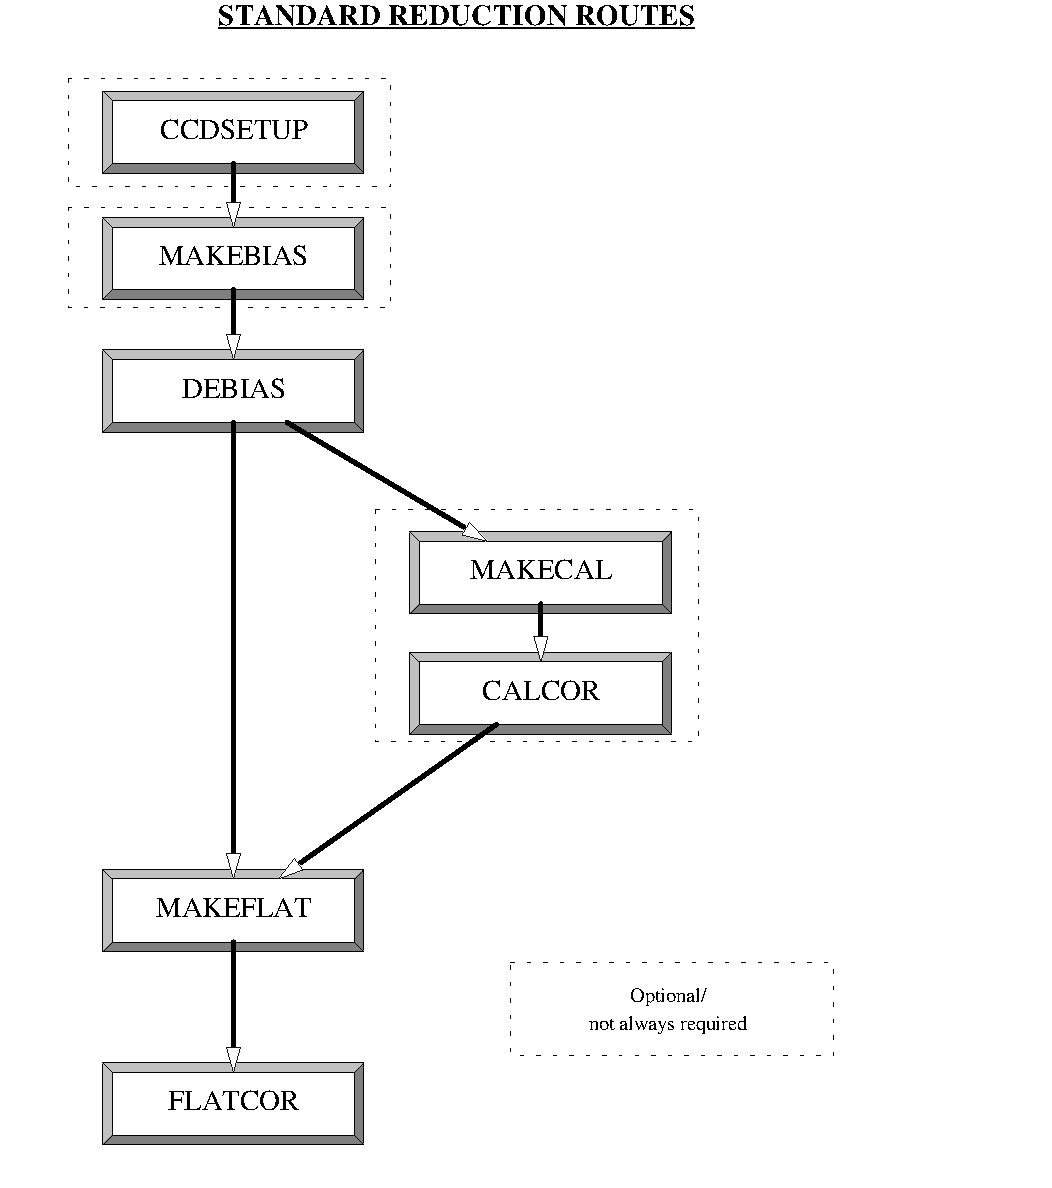
\includegraphics[height=0.85\linewidth]{sun139_red}
\caption[A schematic outline of the order in which CCDPACK reduction
  routines should be used] {A schematic outline of the order in which
  CCDPACK reduction routines should be used.  Dashed boxes indicate
  that this part is optional or not required. The
  \xroutine{MAKECAL}/\xroutine{CALCOR} section may need repeating more
  than once (e.g. if flash and dark frames are to be
  processed). \label{reductionpicture}}
\end{figure}
%  Make sure that this schematic gets printed out now.
\clearpage

\subsection{IR data reduction \label{IRreduction} \xlabel{IRreduction}}

Reducing Infra-Red (IR) array data has many similarities to
reducing CCD data.
The major differences are usually an apparent lack of bias information
(no bias frames or strips) and flatfields, and the need to remove dark
current.

Normally if you have no bias frames then your data should already be
debiassed (this is typically an observing option), in this case unless
you want to remove defective pixels (\htmlref{ARD}{datamasks} files can
be easily generated from a glitch file as it has a PIXEL keyword
 -- see \S\ref{datamasks}),
and/or generate error estimates for your data (the \xref{PHOTOM
-- SUN/45}{sun45}{} package can make use of these), you can miss out
the debiassing stage. If you want to pass your data through \xroutine{DEBIAS} use
the option to subtract a constant as in:
\begin{terminalv}
% debias in='irdata*' out='*_db' usecon zero=0.0
\end{terminalv}

Another way that IR data can be debiassed is by subtracting the bias
contribution at the same time as the dark current (since a dark
current frame must have the same bias contribution).
If you have data like this then you need to use the \xroutine{MAKECAL}
and \xroutine{CALCOR} routines to create a master dark (if you have
more then one dark count frame) and then subtract both contributions
together.
One less obvious point about this method is that you should not use
dark counts that do not have exactly the same exposure as your data
(this is because the bias level doesn't scale, it's an absolute value).

If you have bias frames then follow the normal CCD procedures for
subtracting without bias strips.

The way that flatfielding is usually done with IR array data is by
`dithering' the object frames on the sky (this also makes sure that the
defective pixels are different, relative to the objects) and then
median stacking them.
Of course this will fail if your objects cover a large area of the
detector and the typical contribution in the stack of images isn't sky
at every pixel.
You may of course have some sky frames that can be used as flatfields.

The following script shows how you might reduce you data if you want
to deglitch and generate errors if your data is already debiassed.

\begin{center}
\fbox{Example 7}
\end{center}

\begin{terminalv}
#
#  Clear any existing setup.
#
ccdclear reset accept
#
#  Convert the glitch file into an ARD file.
#
$CCDPACK_DIR/glitch2ard GLITCH.DAT glitch.ard
#
# Debias all the frames using a 0 contribution.
#
debias in='"data*,dark*"' usecon=true zero=0 out='*_db' genvar=false \
       mask=glitch.ard accept
#
# Dark subtraction. Note all dark frames and data frames have the same
# exposures
#
makecal in='dark*-db' out=master_dark expose=1 accept
calcor in='data*_db' cal=master_dark expose=1 out='*_dk'
#
# Median filter of the debias&dark corrected frames to produce the
# flatfield.
#
makeflat in='*_dk' method=median out=master_flat accept
#
# Now flatfield all frames.
#
flatcor in='*_dk' flat=master_flat out='*-fl'
#
# The next step is to mosaic the frames, using PAIRNDF, REGISTER,
# TRANNDF and MAKEMOS routines...
\end{terminalv}

A copy of this file is available from
\text{\$CCDPACK\_DIR} in the file \text{ccdpack\_ex7.csh}.

Automated reductions are also possible for IR array data. The
following script shows how to reduce data that has already been
debiassed and uses the object data frames to produce a flatfield.

\begin{center}
\fbox{Example 8}
\end{center}

\begin{terminalv}
#!/bin/csh
#
#  Initialise ccdpack
#
ccdpack
#
#  Clear any existing global parameters.
#
ccdclear reset accept
#
#  Convert the glitch file into an ARD file.
#
$CCDPACK_DIR/glitch2ard GLITCH.LIST glitch.ard
#
#  Set some global preferences.
#
ccdsetup logto=terminal genvar=true mask=glitch.ard reset accept
#
#  Present the darks, H, J and K data to CCDPACK.
#
present target='"^hframes,^darks"' onefilter filter=h modify \
        adddark onedarktime darktime=1 biasvalue=0 reset accept
present target=^jframes onefilter filter=j modify adddark \
        onedarktime darktime=1 biasvalue=0 reset accept
present target=^kframes onefilter filter=k modify adddark \
        onedarktime darktime=1 biasvalue=0 reset accept
#
#  Now reduce all that data.
#
schedule in='"^hframes,^jframes,^kframes,^darks"' irflats=true \
         execute=true debias=4 spacesave=some reset accept
#
exit
\end{terminalv}
A copy of this file is available from
\text{\$CCDPACK\_DIR} in the file \text{ccdpack\_ex8.csh}.



\section{Registration and mosaicing\label{mosaicing}\xlabel{mosaicing}}

Multiple observations form the backbone of many astronomical programmes.
Determining the registration (inter-dataset transformations) of the
observations is a necessary step when preparing to inter-compare or
combine the data. Inter-comparison is used when performing multiple
waveband observations; combination when measurements beyond the
capabilities of the detector are required. Helping astronomers to
determine the registration of imaging data and subsequently to transform
positions or resample and combine the data is the purpose of this part
of CCDPACK.

A number of registration techniques are provided, which can
identify the relative positioning of frames by examining image
features (centroidable objects), or by making use of prior information
about the observational geometry, or both.

If it is the intention to combine datasets
into one (to increase signal to noise levels, or to increase the
effective area or dynamic range of the detector) the registering
transforms may be used to resample the datasets so they are aligned
(i.e.\ have pixel-to-pixel correspondence).  If atmospheric
transparency, sky brightness or exposure times have varied between the
datasets, they need to go though a process of `normalisation', in
which global zero points and scale factors are determined. After these
stages the data may be combined to produce a mosaic. Data combination
usually makes use of a robust estimator to protect against spurious
values, cosmic rays etc.

{\em
Version 3 of CCDPACK, which was released in mid-2000,
handles the registration process
differently from previous versions --- instead of using TRANSFORM
structures it now normally makes use of World Coordinate System
(WCS) components of the images.  For much of the time, and in particular
to do the things which CCDPACK used to do, it is not
necessary to be aware of this, but it opens the way to some new
functionality.
Discussion specific to the old methods can be found in
appendix \S\ref{transformreg}.
}


\subsection{\xlabel{registrationprocess}\label{regproc}The registration process}

Registering a set of images requires identifying a single
coordinate system which can apply to all of them, so that
each pixel in each of the images has a definite position in
the overall picture as well as within its own grid.
This single coordinate system within which all the images can
be embedded may be an actual sky coordinate system with RA and
Dec coordinates, or an arbitrary one which coincides with the
pixel coordinates of one of the images, or some other kind.
Information on how to embed the images in the same coordinate
system may come from one or more of a variety of sources,
for instance:
\begin{description}
\item[Telescope pointing information:]
The telescope system may insert FITS headers recording the
position in the sky from which the observation was taken.
Alternatively, this could simply be encoded in the filename or
known to you in a non-machine-readable form.
\item[Mosaic camera geometry:]
If the instrument is a mosaic camera in which several CCD chips
are adjacently positioned on the focal plane,
then one observation will comprise a set of related image files,
whose relative positions may be known.
\item[Multiple exposures:]
If multiple exposures are taken without moving the telescope
or otherwise altering the observational setup,
then trivially the images in question will share the same coordinate
system.
\item[Object matching:]
When a number of images overlap and the same features
appear in more than one of them, the relative positioning
of the images can be determined by matching up the features.
\end{description}
For a given set of data,
some of these sources may be more accurate or reliable than others.

It is possible to attach any number of these coordinate systems
to an image.  Once all the images that you are interested in
have the same coordinate system attached to them, then
they can all be resampled so they match pixel for pixel,
ready for combination or comparison.
There are two ways of keeping track of which coordinate systems
are attached to an image: firstly, each coordinate system has a label
(sometimes called its {\em domain\/}) which can be used to identify it.
Some of these
labels have special meaning, for instance a coordinate system labelled
`SKY' indicates
positions on the sky itself and coordinates are usually reported in
RA and Dec
(the other special labels are GRID, PIXEL and AXIS).
Secondly, an image
always has a {\em Current\/} coordinate system, which is the
one in which positions are normally reported.
These attached
coordinate systems are understood by other Starlink applications
so that for instance using KAPPA's
\xref{DISPLAY}{sun95}{DISPLAY} command:
\begin{terminalv}
% display myimage axes
\end{terminalv}
will display \texttt{myimage} with axes showing coordinates from
the Current system attached to the image.

CCDPACK provides four main categories of facility
for adding coordinate systems to sets of images,
which are described later in this section as follows:
\begin{description}
\item[Object matching methods:]
\routine{FINDOBJ}, \routine{FINDOFF}, \routine{PAIRNDF}, \routine{CCDALIGN}
and \routine{REGISTER} are described
\slhyperref{here}{in \S}{}{object_matching}.
These are suitable if you have a set of mutually overlapping images
which can be aligned by identifying the same objects in different images.
%
\item[Direct manipulation of coordinate systems:]
\routine{WCSEDIT} is decribed
\slhyperref{here}{in \S}{}{wcsdirect} and
can be used to examine coordinate systems attached to an image,
add them, remove them, or change which one is Current for an image when
it's necessary to do this manually.
%
\item[Dealing with externally stored coordinate systems:]
\routine{ASTIMP} and \routine{ASTEXP} are described
\slhyperref{here}{in \S}{}{astfiles}.
These allow coordinate system information to be saved in and restored
from external files, and can be used to align multiple sets of images
in the same way relative to each other --- this can for instance be
used for observations from mosaic cameras.
The \routine{MAKESET} command can also be used to read coordinate
information from an external files ---
see the section on dealing with Sets (\ref{ccdpack_sets}).
\
%
\item[Combining information from existing coordinate systems:]
\routine{WCSREG} is described
\slhyperref{here}{in \S}{}{wcscombine},
and can be used to produce a unified coordinate system out of several
present in a set of images when this is possible.
\end{description}
Resampling and mosaicing registered images is discussed in
sections \S\ref{resampling}, \ref{mos_norm} and \ref{drizzling},
and some examples of putting it all together are given in
\S\ref{regexamples}.


\subsubsection{More about attached coordinate systems}

The discussion elsewhere in this document tells you all
that you need to know
for using coordinate systems attached to image files
in order to register them within CCDPACK.
In fact for simple cases in which images are to be registered using,
for instance, only object matching methods, it is not necessary to
understand how the coordinate systems are handled by the registration
programs.
However, you can get a better understanding of coordinate systems
and what you can do with them (including using them for image display)
in the ``\xref{Using World Coordinate Systems}{sun95}{se_wcsuse}''
section of the KAPPA document, \xref{SUN/95}{sun95}{},
and more detailed description of the underlying AST system in
\xref{SUN/210}{sun210}{}.

In general CCDPACK conforms to the normal rules about World Coordinate
System (WCS) image components and AST objects
so other applications, for instance
KAPPA's \xref{WCSTRAN}{sun95}{WCSTRAN} and friends, can freely
be mixed with CCDPACK applications.  In fact some of the KAPPA
applications provide similar facilities to those of the CCDPACK
ones, and they can be used instead if for some reason you prefer
them.
There are a couple of additional conventions used within CCDPACK however:
\begin{itemize}
\item
Some of the CCDPACK applications attach
new coordinate systems to images,
and these are normally given a domain (label)
starting with the characters `CCD\_'.
Thus it is not a good idea to pick a domain which begins `CCD\_'
if you are assigning one yourself, unless you intend it to look
like an automatically generated one.
The special domains which are currently used by CCDPACK are as follows:
\begin{description}
\item[CCD\_REG]
The object-matching alignment coordinates
found by the \xroutine{REGISTER} program.
\item[CCD\_WCSREG]
The global alignment coordinates found by the \xroutine{WCSREG} program.
\item[CCD\_SET]
The alignment coordinates inserted by the \xroutine{MAKESET} program
denoting a Set; this has special significance to most of the registration
programs.
\item[CCD\_OLDPIXEL]
A copy of the pre-transformation PIXEL coordinates stored by the
\routine{TRANNDF} task stored in the transformed image.  This is
not subsequently used by CCDPACK, but may be useful for comparing
the old and new coordinate systems.
\item[CCD\_GEN]
The coordinates in which images are generated by the \routine{CCDGENERATE}
program.  This program is not documented but is used to generate the
test data used in the demomstration scripts.
\item[CCD\_REG1]
Used internally by \xroutine{CCDALIGN}.
\end{description}

\item
Although there is nothing to prevent multiple coordinate systems
in the same image having the same domain, this is likely to lead
to confusion.  CCDPACK will usually try to ensure that multiple
coordinate systems with the same domain do not exist by deleting all but one.
In this case a warning will be issued, but it is not considered
a fatal error.
For instance, the \routine{REGISTER} program normally attaches a new
coordinate system labelled `CCD\_REG' to the images on which it operates;
If any of them already has a coordinate system labelled CCD\_REG,
then the old one gets deleted, and you will be warned that this
has happened.
\end{itemize}



\subsection{\xlabel{objectmatching}\label{object_matching}Object matching
            and position lists}

In CCDPACK three methods for determining image feature correspondence
are provided. Two of these rely on transformations between
coordinate systems being
`well modelled' by simple offsets. These methods have the advantage of
automated and semi-automated processing. The third method relies on
considerable interaction but can deal with transformations of scale,
magnification and shear as well as offsets (i.e.\ general linear
transformations).

If images are well modelled by simple offsets apart from a
{\em known} transformation, for instance a rotation of the
instrument between observations, then a coordinate system
describing the known
transformation can be added using \xroutine{WCSEDIT} or \xroutine{ASTIMP},
and the automated methods still used.


\subsubsection{\xlabel{registration}\label{registration}Determining
               transformation parameters}

The routine which determines the transformations between labelled
position lists is called:
\begin{itemize}
\item \xroutine{REGISTER}.
\end{itemize}
Labelled position lists are those in which the same objects (image
features) have the same identification number. So for instance if a
star say no.\ 100 is present on several datasets it should be labelled
no.\ 100 (or any other unique value) in all the datasets in which it
appears {\em regardless of its coordinates}. In many ways getting
labelled position lists may be considered as most of the process of
object-matching-based registration,
the rest being essentially straight-forward.

The main mapping used by \routine{REGISTER} is the linear mapping:
\begin{terminalv}
XX = A + B * X + C * Y
YY = D + E * X + F * Y
\end{terminalv}
where the \text{A-F} are the coefficients which are to be
determined, \text{X} and \text{Y} the current coordinates and
\text{XX} and \text{YY} the new coordinates. \routine{REGISTER} supports
various types of linear transformations namely:
\begin{itemize}
\item a shift of origin
\item a shift of origin and rotation
\item a shift of origin and magnification
\item a shift of origin, rotation and magnification (solid body)
\item or a full six parameter fit.
\end{itemize}

When using a linear fit you can register a {\em whole\/} list of datasets
in one go. So for instance if you have a set of position lists in which
corresponding objects have been identified, you may pick any list as the
reference set (the first is chosen by default) and all the mappings between
this and the other datasets will be derived.
If the position lists are `associated' with images then a new
coordinate system,
by default labelled `CCD\_REG', will be added to each image:
the coordinates are the same as
the pixel coordinates of the reference image.

A general transformation between {\em two\/} datasets can also be
determined. These are entered using suitably parameterised algebraic
expressions. A general least squares fitting algorithm is used to find
a solution which gives satisfactory values for the parameters.



\subsubsection{\xlabel{automatedregistration}Automated registration
               \label{automatedregistration}}

If the coordinates of your images are just offset from each other
(related by a translation in X and Y)
and they have image features in
common it may be possible to register them with a minimum of effort and
preparation.
More precisely, the relation between coordinates does not have to
be exactly an offset, but to be
sufficiently `well modelled' by an offset, that is
with distorting terms small enough that the error in
positioning is in general a larger effect.

Automated registration is performed by the applications:
\begin{itemize}
\item \xroutine{FINDOBJ}
\item \xroutine{FINDOFF}
\item \xroutine{REGISTER}
\end{itemize}
used in that order.

\routine{FINDOBJ} locates and centroids image features,
\routine{FINDOFF} determines the
correspondence of the image-features and \routine{REGISTER} produces the
mappings from this information. This sequence is used in the
demonstration script
\slhyperref{\texttt{ccdexercise}}{\texttt{ccdexercise} described in \S}{}{demos}.

\routine{FINDOBJ} works by looking for pixels above a threshold value,
objects are
then identified as groups of `connected' pixels. The groups of connected
pixels are then centroided to give an accurate position.
\routine{FINDOBJ} has a number of parameters which can be tweaked
to identify a suitable group of objects from the data;
however if you can't make it work satisfactorily you could use
the interactive program \xroutine{IDICURS} instead for this step.

\routine{FINDOFF} is the crucial application in this sequence, it performs
pattern-matching between all the object positions. It assesses the
degree of match found between each pair of frames and assigns it a
weight. The best matches are then used to identify corresponding objects
on each frame.  The inter-comparison process which provides the
pattern-matching facilities uses two algorithms, one which matches
{\em all} the point pair-offsets between any two input lists, counting
all the other points which are then paired (within an error box).  The
match with the most positions paired is then chosen. The second  uses a
statistical algorithm based on histograms of the differences in the
offsets (where the peak in a histogram is assumed to be the most likely
difference). In each case an estimate of the positional error must be
given as it is used when deciding which positions match or as the bin
size when forming histograms.

Which algorithm you should use depends on the number of points your
position lists contain and the expected number of objects in the
overlaps. Obviously it is much easier to detect a match between  two
lists which have most of their positions in common. With small overlaps
a serious concern is the likelihood of finding a `false' match. False
matches are more likely the larger the datasets and the smaller the
overlaps.

The first algorithm (named SLOW) is the most careful and is capable of
pairing positions in data with small overlaps (although a level of false
detections will always be present) but the process is inherently slow
scaling as $N^{3}\ln_{2}N$. The second algorithm (named FAST) is an
$N^2$ process so is much quicker, but requires better overlap
statistics. The {\em maximum} time taken for determining the
correspondence of two position lists for the SLOW algorithm are shown in
table \ref{table1}. If you intend to process large lists then take heed.

\begin{table}[htb]
\begin{center}
\begin{tabular}{|c|c|c|c|c|c|}
\hline
$N$ & $50$ & $100$ & $250$ & $500$ & $1000$\\
\hline
Time (seconds) &
     $0.5$ & $2.5$ & $53$ & $535$ & $5800$\\
\hline
\end{tabular}
\caption{Maximum time taken to process two lists of $N$ points.
The tests were run on a DEC Alpha 3000/300.
\label{table1} }
\end{center}
\end{table}

Because the FAST process takes so little CPU time it is better to try
this first (without the SLOW process as a backup,
FAILSAFE=FALSE), only use the SLOW algorithm when you have
small datasets or do not have large overlaps.

Having obtained estimates of the offsets between each dataset pair and
the number of positions in common, the next stage is to determine a
{\em global} solution to the registration of all the datasets. A major
consideration is the possible presence of false matches.

The global registration process works by forming a graph with each
position list at a node and with connecting edges of weight the number
of matched  position-pairs. The edge weights may be modified by a
completeness factor which attempts to assess the quality of the match
(this is based on the ratio of the expected number of matches in the
overlap region to the actual number, random matches shouldn't return
good statistics when compared with genuine ones). This still leaves a
possibility of false matches disrupting any attempt to register the
datasets so a single `spanning tree' is chosen (this is a graph which
just visits each node the minimum number of times required to get
complete connectivity, no loops allowed) which has the highest possible
number of matched positions (rejecting edges with few matched
positions/low completenesses where possible). This gives a most likely
solution to the offsets between the position lists, rather than the
{\em best} solution which could well include false matches; compare this
with a median as opposed to a mean. This registration is then used to
identify objects in all datasets, resulting in {\em labelled} position
lists which are output for use by \routine{REGISTER}.

Note it is not necessary that the pixel grids of the images are simply
related by an offset,
but that their Current coordinate systems are.
For instance you might have two images with reasonably accurate
SKY coordinate systems which were attached by the observing system,
but which you wish to register more accurately by matching image features.
The telescope was rotated as well as
shifted between the observations so that the
X-direction of one data array is different from the X-direction of
the other.  But since the SKY coordinate system of each only
has small errors, the RA-direction of each is the same.
Then as long as SKY is the Current coordinate system,
the methods in this section can be used to align the images automatically
(see section \S\ref{regexamples} for an example).
If you know the non-offset parts of the transformation
but they are not already present as attached coordinate systems,
then you may be able to add them yourself using \routine{WCSEDIT}
or \routine{ASTIMP} as explained in later sections.

Invoking \xroutine{FINDOBJ}, \xroutine{FINDOFF} and
\xroutine{REGISTER} is simple.
\begin{terminalv}
% findobj in='*' outlist='*.find'
% findoff inlist='*' outlist='*.off' error=1
% register inlist='*' fittype=1
\end{terminalv}
This locates the objects on all the images in the current directory,
performs pattern-matching and finally registers them, attaching
a new coordinate system labelled `CCD\_REG' to each image.
See ``\slhyperref{Using position lists}{\S}{}{using_position_lists}''
if using `\text{*}' for both the IN and INLIST
parameters seems mysterious.

If the coordinates of the images are already quite well matched
(offsets are expected to be small)
and the object matching is just to improve the alignment,
then \routine{FINDOFF} can be invoked with the RESTRICT parameter;
this instructs it to look for matching objects only in the
parts of the images which overlap according to the existing
Current coordinate system, which can dramatically decrease running time
and the likelihood of a false match.

\routine{FINDOFF}'s other parameters are detailed in
\slhyperref{a later section}{\S}{}{FINDOFF} and some of its internals are
explained in P.W. Draper, {\bf 1993}, `Preparing multiple CCD frames for the
photometry of extended fields', Proceedings of the 5th ESO/ST-ECF Data
Analysis Workshop.



\subsubsection{\xlabel{semiautomated}\label{semiautomated}Semi-automated
               registration}

When datasets are offset in their Current attached coordinate system
only by X and Y translations as above,
but contain insufficient objects for the fully automated registration
described in the previous section,
registration may be done in a semi-automated way,
using the programs:
\begin{itemize}
\item \xroutine{PAIRNDF}
\item \xroutine{REGISTER}
\end{itemize}

\routine{PAIRNDF} displays the images to be registered and allows the direct
selection of image features which are common between image pairs.
This works by asking you alternately to choose a pair of images
which has an overlap, and then to line them up.
When enough of the datasets have been selected this way, and
successfully paired, the global correspondence of the image features
is determined. Using this method avoids the need to identify each
image feature in a particular sequence, they are just selected as
being in `common' between any pair, \routine{PAIRNDF} works out the rest using
the same methods as \xroutine{FINDOFF}, except a single spanning tree is not
chosen since in this case, all pairings are assumed to be correct.

Both the pair selection and the pair alignment are done using an
intuitive graphical user interface on the Xwindows display.
During pair selection you can see any combination of
two images side by side, along with their names and other information
such as selected FITS headers.  They are displayed resampled into
their current coordinate frames, so that it should be easy to see
where any overlap between the two is.  When you have selected a pair
which contains objects common to both, you can move to
the alignment stage
in which you drag one image with the mouse to the correct position
on top of the other.
The display can be zoomed and scrolled to make careful positioning easy.
You are then asked to select centroidable features in the
overlap region so that the program
can determine the offset between the two accurately.

To summarise, during the graphical part of \routine{PAIRNDF}
you have to do the following:
\begin{enumerate}
\item Select a pair with features in common
\item Align them by dragging and dropping
\item Mark objects in the overlap region
\item Repeat until the program stops asking you to do so \\
      {\em or\/}\\
      Click the `Exit' button when you cannot make any more pairings
\end{enumerate}
If in the final step you select Exit yourself rather than pairing all
the images, then \routine{PAIRNDF} will not be able to register
all the datasets.  In this case it will behave the same as
\xroutine{FINDOFF}, which is to do all the alignment it can,
and associate position lists with those files whose alignment it
can work out.
Running \routine{REGISTER} will then add coordinate systems only
for those which you have paired, and you will have to align the
others in a different way, perhaps with the help of \xroutine{WCSREG}.

As with all graphically based interfaces it is difficult to
describe the advantages and ease of use, it's best to try them out.


\subsubsection{\xlabel{usinglineartransforms}General linear transformations
               \label{usinglineartransforms}}

To align datasets that require more general linear transformations
than a simple offset
use the:
\begin{itemize}
\item \xroutine{CCDALIGN}
\end{itemize}
procedure. This accepts either a sequence of images or related images
(datasets which are already approximately aligned, at least within the
capabilities of centroiding $\approx$ few pixels) and displays them one
by one (or the first member of each group). You then have to simply
identify the image features to use, but in the correct order. Only
enough image features to identify the approximate image position are
required as the  procedure then centroids the image features, works out
an approximate registration which it then uses to extrapolate the
positions of a reference set on each dataset. This new extended set of
positions are now centroided picking up any missed objects. The
reference set of positions are either selected from a designated image or
from the first image.
\routine{CCDALIGN} can then invoke \routine{REGISTER} itself to
perform the fitting of the transformation parameters using all these
positions.

Selection of points on the images is done using an inuitive Xwindows-based
graphical user interface, which allows you to mark and remove
points with the mouse, change the brightness of the display,
zoom and scroll the image, and read out positions in any
of the image's attached coordinate systems.

To summarise, during the graphical part of \routine{CCDALIGN}
you have to do the following:
\begin{enumerate}
\item Mark a set of points on the reference (or first) image
\item Mark corresponding points on each of the other images
\end{enumerate}



\subsubsection{\xlabel{usinglistsofpositions}Using position lists
               \label{using_position_lists}}

In CCDPACK the positions of identified/detected image features are
stored in ordinary text files which are referred to as `position lists'.
The format of these lists is flexible. Usually position lists have three
columns:
\begin{terminalv}
Identifier    X-position    Y-position
\end{terminalv}
these may be separated by commas or blanks. The identifier is an
integer value which is used to identify positions which are related
(i.e.\ are of the same object) in different lists.

If more than three columns exist then only the values in the first
three are used, though some of the programs propagate extra columns
from the input to the output lists.
If only two columns exist it is assumed that they are:
\begin{terminalv}
X-position    Y-position
\end{terminalv}
such lists may be produced by \xref{KAPPA}{sun95}{} applications. In
this case applications which rely on a knowledge of the identifiers
assume they are monotonically increasing from one.

Whole and in-line comments are allowed in position lists using the
character `\texttt{\#}'.  These are not propagated from input to output lists.
Note that the final line of the file should be terminated by a
newline character (certain text editors do not always enforce this).

The X and Y values in a position list always refer to the
pixel coordinates of an image.
When \routine{FINDOFF} or \routine{REGISTER} read them they
automatically transform them into the Current image coordinate system
where appropriate.
For this reason there is not normally any need to transform a position
lists the corresponding image has been resampled;
however if necessary it can be done using the
\xroutine{TRANLIST} routine.  This is discussed, along with the
methods that previous versions of CCDPACK used
for storing coordinate transformations,
in appendix \ref{transformreg}.

Usually position lists are `associated' with images. What this means is
that when a position list is created a record of its name is kept in the
extension of the image. It is then usual to refer to the image instead of
the position list when the position list is to be accessed. Applications
which create new position lists associate the new position lists with
the appropriate image. Using this method avoids any confusion about the
relationship of position lists and images, which is vital when determining
the registration of many images at one go. It also allows the use of the
wildcarding properties of image names to access position lists.

The association of position lists can be disabled completely by setting
the NDFNAMES global parameter
(\xroutine{CCDSETUP}) to false. In this case, position lists must be specified
explicitly as a comma separated list of names or gotten from a text
file using indirection, this is exactly the same as for naming images
(see ``\slhyperref{processing lists of data}{\S}{}{ndflists}'') except that
wildcards are {\em not} allowed. Output list names may be formed
from the modification of these names when NDFNAMES is false, otherwise
the input image names are {\em always} used.

The name of the position list associated with an image is stored
in its .MORE.CCDPACK extension under the item CURRENT\_LIST, and
can be examined using \xref{HDSTRACE (SUN/102)}{sun102}{}
or modified using \xroutine{CCDEDIT}.

If you wish to view or edit positions in a list interactively,
you can use the \xroutine{IDICURS} program, which displays a
graphical interface in
which the image is displayed with points from a position list
plotted over it.  Points can be added and removed with the mouse.
If you want to display points in a list non-interactively or
to print them out, use \xroutine{PLOTLIST}.


\subsection{\xlabel{wcsdirect}\label{wcsdirect}Handling coordinate systems
            directly}

CCDPACK provides the routine
\begin{itemize}
\item \xroutine{WCSEDIT}
\end{itemize}
for direct manipulation of the coordinate system information attached
to an image or a group of images.
It can examine, add, remove or modify coordinate systems,
and select the coordinate system to be regarded as Current.

To examine the coordinate systems attached to an image, you
can use \routine{WCSEDIT} with the parameter MODE set to SHOW;
for example:
\begin{terminalv}
% wcsedit obs1 show

    WCSEDIT
    =======
  1 NDF accessed using parameter IN

    Index Cur  Domain            Title
    ----- ---  ------            -----

obs1:
      1        GRID              Data grid indices; first pixel at (1,1)
      2        PIXEL             Pixel coordinates; first pixel at (0.5,0.5)
      3        AXIS              Axis coordinates; first pixel at (0.5,0.5)
      4    *   SKY               FK5 equatorial coordinates; mean equinox...
      5        CCD_REG           Alignment by REGISTER
\end{terminalv}
This shows that there are five coordinate systems in the image and
that number~4, labelled `SKY' is the Current one.
Note that the first three coordinate systems attached to an image
are always GRID, PIXEL and AXIS.
SKY is not always present but if it is, it should always represent
a celestial coordinate system.
GRID and PIXEL always have units the same size as that of a pixel
(the difference is that GRID is guaranteed to start at (1,1)).

For the other modes (add, remove, current and set) of \routine{WCSEDIT}
you need to specify a given coordinate system,
the `target', for \routine{WCSEDIT} to work with.
This is given using the FRAME parameter, and you can use one
of the following formats:
\begin{itemize}
\item
The null value (`\texttt{!}'), indicating the Current coordinate system
\item
The domain (name) of the coordinate system
\item
An integer giving the index of the coordinate system
\item
A \qt{Sky Co-ordinate System} (SCS) value such as EQUAT(J2000)
(see section ``\xref{Sky Co-ordinate Systems}{sun95}{se_scs}'' in
\xref{SUN/95}{sun95}{}).
\end{itemize}
The first two options are usually the most appropriate.
As you can see above, the output of `\texttt{wcsedit show}'
will show you what domains there are, what the index of each is,
and which coordinate system is Current for a given image.

To change the coordinate system to be used as the Current one
therefore, simply write something like:
\begin{terminalv}
% wcsedit in='image*' mode=current frame=pixel
\end{terminalv}
or just
\begin{terminalv}
% wcsedit 'image*' current pixel
\end{terminalv}
which will set the Current coordinate system of all the image files
indicated to pixel coordinates.
Since the PIXEL coordinates are in some sense the native ones,
if you set Current to PIXEL in this way
the images will behave in most respects as if they had no attached
coordinate systems at all.

Syntax for removing coordinate systems is much the same:
\begin{terminalv}
% wcsedit image remove 4
\end{terminalv}
will remove the fourth (as listed by \texttt{wcsedit show}) coordinate
system from file \texttt{image}.

When adding a new
coordinate system you must give the transformation which connects it
to the target coordinate system.
The transformation can be one of the following types:
\begin{description}
\item[UNIT:]
No coordinate transformation is performed in this case.
A copy of an existing coordinate system, but with a new domain (label),
can thus be added in this way.
\item[LINEAR:]
A general linear tranformation can be specified by giving six
coefficients $C_{1-6}$:
\begin{eqnarray*}
   x^\prime & = & C_1 + C_2 x + C_3 y \\
   y^\prime & = & C_4 + C_5 x + C_6 y
\end{eqnarray*}
\item[PINCUSHION:]
A pincushion-type transformation,
which is a common optical distortion,
can be specified by giving three coefficients $C_{1-3}$,
the magnitude of the distortion followed by the coordinates of its centre:
\begin{eqnarray*}
   x^\prime = x \left( 1 + C_1  \left[ \left( x - C_2 \right)^2
                                     + \left( y - C_3 \right)^2 \right] \right)
   \\
   y^\prime = y \left( 1 + C_1  \left[ \left( x - C_2 \right)^2
                                     + \left( y - C_3 \right)^2 \right] \right)
\end{eqnarray*}
A positive $C_1$ corresponds to a pincushion distortion and
a negative $C_1$ corresponds to a barrel distortion.
\item[MATH:]
An arbitrary algebraic transformation.
In this case you will be asked to specify the mapping between coordinate
systems using a FORTRAN-like syntax.
\end{description}
So the following command would
add a new coordinate system, labelled `SQUASHED',
representing a barrel distortion of the coordinates labelled `FOCAL'
having a magnitude of $7\times 10^{-6}$
and an optical centre at coordinates (1000,1000):
\begin{terminalv}
% wcsedit 'image*' add frame=focal domain=squashed maptype=pincushion
          coeffs='[-7e-6,1000,1000]'
\end{terminalv}

It's also possible to make fine adjustments to the coordinate
systems attached to an image using the SET mode, for example:
\begin{terminalv}
% wcsedit file1 set frame='!' set='domain=obs1'
\end{terminalv}
changes the name of the Current coordinate system to `OBS1'.
For more sophisticated use of this feature, see the documentation
of \xroutine{WCSEDIT} in appendix \S\ref{app:description}, and of
the \xref{AST\_SET}{sun210}{AST\_SET} routine in \xref{SUN/210}{sun210}{}.

When run, \routine{WCSEDIT} will log what it has done,
giving the domain of the altered coordinate system where appropriate
(even if it was specified in some other way).
If it could not perform the requested action on any of the images
in the list, an appropriate message will be written, but this
does not consitute a fatal error.
However, it does write an list to an output file (by default called
WCSEDIT.LIS), giving the names of only those images
which were successfully accessed, which normally
means those which had a coordinate system matching that
given by the FRAME parameter.  So it's easy to find out which
images were successfully modified:
\begin{terminalv}
% wcsedit 'data?' current focal

    WCSEDIT
    =======
  4 NDFs accessed using parameter IN

data1: Current frame set to domain FOCAL

data2: Target frame 'focal' not found
       NDF not modified

data3: Current frame set to domain FOCAL

data4: Current frame set to domain FOCAL

% cat WCSEDIT.LIS
data1
data2
data4
\end{terminalv}
This name list file can be used as an indirection file to pass to the
input of another CCDPACK task.  For instance, if you want to do an
interactive alignment of only those files which have coordinate
systems with the name ``FOCAL'', you could follow the above command
with this:
\begin{terminalv}
% pairndf '^WCSEDIT.LIS'
\end{terminalv}



\subsection{\xlabel{astfiles}\label{astfiles}Re-use of coordinate system
            information with AST files}

Coordinate systems can be exported from and imported to
image files using the commands:
\begin{itemize}
\item \xroutine{ASTEXP}
\item \xroutine{ASTIMP}
\end{itemize}
(the \xroutine{MAKESET} routine can be used as a substitute for
\routine{ASTIMP} if CCDPACK Sets are being used ---
see Section \ref{ccdpack_sets}).

Sometimes the coordinate transformations which must be applied
to one set of observations are the same as those
required for many other sets.
One example of this is the observations from a mosaic
CCD camera, in which multiple CCD chips are fixed adjacently
in the same focal plane to avoid needing a single very large device;
the relative position of each chip to the others
will not change as a function of pointing direction.
Another example is when the optical distortion of an instrument
(at a given wavelength) is known; if this can be applied
correctly to one observation it can be applied to many.
A third example, which is common because the large focal planes
implied by use of a mosaic camera often lead to significant
optical distortions, is the combination of these two.

CCDPACK allows this kind of coordinate transformation information to
be written to (using \routine{ASTEXP}),
and read back from (using \routine{ASTIMP}),
an external file called an AST file.
This effectively stores a coordinate system, and enough information
to graft it onto suitable files, for each one of a related group
of images.
Thus applying the AST file to a set of images adds a new
coordinate system to
each of them, which can be used for the registration process.
Where there are several images in a set, as in the case of
a mosaic camera, \routine{ASTIMP} can determine which coordinate frame to
use for which image either by the order in which they are presented,
or by usng FITS headers in the file,
according to how the AST file was constructed by \routine{ASTEXP}.

Full details on how to use \routine{ASTIMP} and \routine{ASTEXP}
can be found in \slhyperref{an appendix}{appendix }{}{app:description},
but the following gives an example.
\begin{terminalv}
% astexp '"reg_data[1234]"' astfile=inst.ast idtype=fitsid fitsid=chipname
% astimp 'new_data*' astfile=inst.ast
\end{terminalv}
The first command takes a set of 4 images, one from each chip of an array,
which are aligned in their Current coordinate system,
(possibly by object matching)
and constructs a file \text{inst.ast} from them;
the parameters `IDTYPE=FITSID FITSID=CHIPNAME'
mean that the AST file labels each coordinate system with the
value of the `CHIPNAME' FITS header from the \text{reg\_data*} images,
since this dentifies which CCD is which in the mosaic camera.
The second command applies the file \text{inst.ast}
to a set of (any number of) images from the same
instrument which have not yet been registered;
for each one \routine{ASTIMP} works out which coordinate system to
add by matching the `CHIPNAME' FITS header in the image with one of
the ones in the AST file.

If a previously prepared AST file for the instrument you are using
exists, then the \routine{ASTEXP} step can be avoided.
In any case, once a suitable AST file is available,
it can be applied to many sets of images from the same instrument,
as long as the instrument's characteristics remain the same.

There is a more detailed example of the use of \routine{ASTIMP} in
section \S\ref{regexamples}.



\subsection{\xlabel{wcscombine}\label{wcscombine}Combining coordinate systems}

To combine registration information from different sources, you can
use the routine
\begin{itemize}
\item \xroutine{WCSREG}
\end{itemize}

It is not always possible to register a group of images in a single
step, using one kind of procedure.  For instance you might have
a large group of images with an approximate SKY coordinate system
inserted by the observing system,
of which some but not all overlap with each other.
In this case we would like to register the overlapping ones
using the object-matching
techniques described in section \ref{object_matching},
but fall back to
the tolerably accurate SKY coordinates to align the rest of the images.

\routine{WCSREG} can do just this.
You give it a number of images, and a list of coordinate systems
it can use to make the connections,
and if it's possible to align them all using only these coordinate
systems it will do so,
adding a new coordinate system labelled `CCD\_WCSREG' to them all.
In the above example you would write something like
\begin{terminalv}
% wcsreg in='image*' domains='[ccd_reg,sky]'
\end{terminalv}
Where there is a choice between coordinate systems to use for alignment,
ones given earlier in the DOMAINS list are preferred.
The square brackets around the named domains are required here because it
is an array of strings.

The new coordinate system added is a copy of (and so has the same
units as) the PIXEL coordinate system of the reference image,
which is normally the first one listed.
Because of this, if you have
a set of images which are already aligned, but in an
unsuitable coordinate system,
you can align them in a pixel-sized coordinate system using
\routine{WCSREG}.
Giving a null (`!') value for the list of domains will automatically
use the current attached coordinates of the reference image for
alignment, so that running
\begin{terminalv}
% wcsreg in='regdat*' domains='!'
\end{terminalv}
will ensure the group of already registered images \texttt{regdat*}
keeps its existing alignment, but in a coordinate system in
which a unit is pixel-sized.
This can be a useful trick prior to resampling,
since the resampling program \xroutine{TRANNDF} will
resample so that a pixel of the output image is one unit square;
for this reason resampling directly into a SKY coordinate system,
in which a unit is one radian, is bound to give a useless result.

In many cases it will be possible to align a set of images in
one step without worrying about these sorts of procedure.
For the more complicated cases where
coordinate information of varying levels of
accuracy and completeness is available from several
different sources however,
\routine{WCSREG}, in conjunction with the other programs described
in this section, provides powerful facilities for making use of
this information.  Some examples of them at work can be found
in \slhyperref{the examples section}{\S }{}{regexamples}.


\subsection{\xlabel{view-align}\label{view-align}Viewing image alignment}

The previous sections describe various methods for aligning
a set of images in a common coordinate system.
Once this is done, you will usually want to resample and combine
or compare them.
Before, instead of, or after that however, you might want to see
the positions of the images in the aligned coordinates.
You can do this using the application:
\begin{itemize}
\item \xroutine{DRAWNDF}
\end{itemize}
If you give \routine{DRAWNDF}
a list of images which are all aligned in their
Current attached coordinate system, it will plot
outlines of the regions covered by each image file.
In this way it is easy to see
which parts of your data cover which parts of the coordinate space.

There are two basic ways of running \routine{DRAWNDF}, according
to whether the parameter CLEAR is set to TRUE or FALSE.
If CLEAR is TRUE, then the graphics device will be cleared and
the outline of the area covered by each image will be shown.
By default, a set of axes will be drawn as well.
This will
give you a good idea of the alignment of your files relative to
each other, and by examining the axes you can see the absolute
positions too.  It can often be a good idea to do this with
a set of data files before you resample and combine them,
which may be a time-consuming step, just
to check that the alignment looks sensible.
You can see an example of this in Figure \ref{OUTCLEAR}.

\myfig{sun139_outclear}{}{height=0.4\textheight}{OUTCLEAR}{Image
  generated by registering the images and running \texttt{drawndf}}{
This image was generated by registering the images and running the
command:\protect\\
\hspace*{2em}\texttt{drawndf r1059* clear noaxes labname labnum}}

If CLEAR is FALSE however, \routine{DRAWNDF} will try to align the
outlines with an existing picture on the graphics display.
This means that if you have already displayed an image
on your graphics device which shares a coordinate system with
your data files, you can see where they would fit over it.
For instance you could show an image which has SKY coordinates
using KAPPA's \xref{DISPLAY}{sun95}{DISPLAY} program
and then run \routine{DRAWNDF} on a set of data files in the
same region; if their Current coordinates are also SKY
you will be able to see how they map onto the displayed image.
Another useful application is to \routine{DISPLAY}
a mosaic which has been made by combining a set of data files,
then to run \routine{DRAWNDF} on the originals
so it is clear which file has contributed to which part of the mosaic.
To achieve this alignment with previously drawn graphics,
\routine{DRAWNDF} uses the AGI graphics database in
the same way as KAPPA programs;
this is described more fully in \xref{SUN/95}{sun95}{se_agitate}.
You can see an example of this in Figure \ref{OUTSKY}.

\myfig{sun139_outsky}{[ht]}{height=0.5\textheight}{OUTSKY}{DRAWNDF command
with CLEAR=FALSE.}{DRAWNDF
command with CLEAR=FALSE.  This picture was generated by displaying
the sky region and then running the command:\protect\\
\hspace*{2em}\texttt{drawndf "gc6352p1-?" noclear
                  labpos=cf style="width(curves)=2"}}

Finally, \routine{DRAWNDF} can display the actual image data for you.
Unlike KAPPA's DISPLAY program, which always displays
an image as a rectangle whose edges are horizontal and vertical,
perhaps with with non-orthogonal image Current coordinate axes
drawn over it, \routine{DRAWNDF} always plots on a surface in which the
Current coordinate system has horizontal and vertical axes.
The image data array is therefore resampled to fit within the
image bounds as they would appear in these coordinates.
This can give you a good view of what a group of images will
look like when they have been resampled and combined into their
Current coordinates.  Note however that unlike \xroutine{MAKEMOS},
\routine{DRAWNDF} performs no averaging or sophisticated normalisation of
images, so that if two images overlap in their Current coordinates,
all but the last-plotted will be obscured, and the relative
brightnesses may not be right.
When this option is used, the display is always cleared.
An example of a set of frames from a mosaic camera displayed
in this way is given in Figure \ref{OUTIM}.

\myfig{sun139_outim}{[ht]}{height=0.5\textheight}{OUTIM}{DRAWNDF with IMAGE=TRUE.}{DRAWNDF
command with IMAGE=TRUE.  This display was generated using the
command:\protect\\
\hspace*{2em}\texttt{drawndf "r10629?" image=yes}}


\subsection{\xlabel{resampling}\label{resampling}Data resampling}

Data resampling is normally performed by the application:
\begin{itemize}
\item \xroutine{TRANNDF}
\end{itemize}
This resamples an image from pixel coordinates into
its Current coordinate system.
So if a set of images shares a common Current coordinate system
(as added by any of the methods described earlier in this section)
then running \routine{TRANNDF} on them all will enable them to
be compared or combined pixel for pixel.
The transformation between pixel co-ordinates and the Current
co-ordinate system can be of any kind,
so the program has the capability of `rubber-sheeting'.
A restriction is that both the forward and the inverse transformations
must be available. This will only cause problems when using general
transformations; a tractable inverse doesn't often exist.
If you need to resample and you do not have an inverse transformation,
the \xroutine{DRIZZLE} program
may be used instead, though note this is not designed for general
purpose resampling, and is slower than \routine{TRANNDF}.

\routine{TRANNDF} resamples using
one of two different techniques, linear interpolation
or nearest neighbour. Linear interpolation uses two pixels to estimate
the new pixel value, nearest neighbour just uses the nearest pixel. Flux
conservation is available but is only supported for linear
transformations. Variances are resampled in the same way as ordinary
data.

The size of the output images can be estimated from the transformation of
selected boundary positions, which is very useful when transforming whole
lists of images as the output images are made only as big as necessary.

To use \routine{TRANNDF} type something like:
\begin{terminalv}
% tranndf in='*' out='*-trn'
\end{terminalv}
This resamples all the images in the current directory naming the output
images the same as the inputs except that the string `\text{-trn}' is
appended to each output name.
By default \routine{TRANNDF} will guess a size for
the output image, interpolate using nearest neighbour and conserve flux.

Note that \routine{TRANNDF} resamples into the Current coordinate system,
so that each pixel in the output image is a $1.0 \times 1.0$ square
in those coordinates.  Thus the coordinate system in question must be
a suitable one for that purpose.  If it has units of
the wrong size, then a suitable transformation can be made by
adding a new coordinate system with the
\xroutine{WCSEDIT} or \xroutine{WCSREG} programs.
In particular it's no good running \routine{TRANNDF} on a set of
images which have SKY coordinates as Current, since they have
units of radians, which are far too big.
See the example in \slhyperref{the section about WCSREG}{\S }{}{wcscombine}
for how to deal with this.

For a quick look at what the resampled data will look like,
the \xroutine{DRAWNDF} command with IMAGE=TRUE can be used.


\subsection{\xlabel{mosaic_normalise}\label{mos_norm}Mosaicing and
            normalisation}

The tasks of mosaicing and normalisation are normally performed using the:
\begin{itemize}
\item \xroutine{MAKEMOS}
\end{itemize}
program.
\routine{MAKEMOS} is a comprehensive program and has many
capabilities. In its default mode \routine{MAKEMOS}
just combines images using a
selected data combination method (\routine{MAKEMOS} supports several
methods: mean, median, trimmed mean etc.\ \S\ref{combinations}).
In this it is similar to the \xroutine{MAKECAL} routine, but
\routine{MAKEMOS} makes much more efficient use of
memory (it is designed to deal with datasets which may not have much
overlap and which might have a very large output extent, unlike with CCD
calibration data where the overlap will usually be complete).

The other capabilities of \routine{MAKEMOS} are concerned
with data normalisation.
Normalisation is determined as two components, a scaling factor and a
zero point factor. These may be controlled independently by the
parameters SCALE and ZERO. So:
\begin{terminalv}
% makemos in='*' out=mosaic scale
% makemos in='*' out=mosaic zero
% makemos in='*' out=mosaic scale zero
\end{terminalv}
would determine just scale factors, just zero points or both scale
factors and zero points respectively. The option also exists to modify
the data values of the input datasets so that their values are
normalised (this may be combined with producing a mosaic or not using
the OUT parameter). A full description of \routine{MAKEMOS}
is given in appendix \S\ref{MAKEMOS}, some of the philosophy of
its algorithms are explained in R.F.~Warren-Smith, {\bf 1993},
`The Calibration of Large-Field Mosaics', Proceedings of the 5th
ESO/ST-ECF Data Analysis Workshop.


\subsection{\label{drizzling}\xlabel{drizzling}Combination by drizzling}

In most cases resampling and mosaicing should be done using
\routine{TRANNDF} and \routine{MAKEMOS}, but for certain specialised
applications the
\begin{itemize}
\item \xroutine{DRIZZLE}
\end{itemize}
program may be superior.
It combines resampling and mosaicing in one task
and the resampling is done using the Variable-Pixel Linear Reconstruction
(or informally ``drizzling'') algorithm.

This algorithm was originally developed for the Hubble Deep
Field, a project whose purpose was to image an otherwise unexceptional
region of the sky to depths beyond those of previous astronomical images.
Its primary application is to provide a method for the linear
reconstruction of an image from a set of undersampled dithered data;
it preserves photometry and resolution, and can weight input images
according to the statistical weight of each pixel.

The input grid is mapped onto an output grid which is normally
finer; where many dithered input images are being combined this
allows subsampling of the input data.
Before the pixels are resampled onto the output grid however,
they are shrunk into smaller pixels, now referred to as ``drops'',
which rain down onto the output grid.
Each drop affects the pixels in the output grid which it covers
in proportion to the area of overlap; if an output pixel is
not touched by any of the drops it receives no data from the image.
This is shown schematically
in \slhyperref{the figure}{figure }{}{drizzlepicture}.

\myfig{sun139_driz}{}{height=0.5\textheight}{drizzlepicture}
{A schematic representation of Drizzling.}{A schematic representation of Drizzling. The input pixel grid
(shown left) is mapped onto a finer output grid (shown right).
Each input image only affects the output pixels under the drops,
so that here the central output pixel recieves no information
from that image (Fruchter \& Hook, ADASS VI,
ASP Conf.\ Series, Vol.\ 125, 1997, G.~Hunt and H.E.~Payne, eds., pp.\
147--150).}

The transformation of input grid to output grid is basically the
transformation between the pixel coordinates and Current coordinates
of the image file;
however an additional shrinking
factor can for convenience be given using the MULTI
parameter of DRIZZLE.  The ratio of the linear size of the
drop to the size of the input pixel is controlled by the
parameter PIXFRAC.  The default values for these
parameters are 1.5 and 0.9 respectively.

The algorithm has a number of advantages over the resampling and
combination methods provided by \routine{TRANNDF} and \routine{MAKEMOS}.
Since the area of the
pixels scales with the Jacobian of the geometric transformation, the
algorithm preserves surface and absolute photometry. Flux can therefore
be measured using an aperture whose size is independent of position on
the output frame. As the algorithm anticipates that output pixels may not
receive data from a given input pixel, bad pixels do not cause significant
problems, so long as the stack of input images is sufficient to fill
in the gaps caused by these zero-weight input pixels. Shifts of a few
pixels between input images therefore allow the user to remove small scale
defects such as hot pixels, bad columns and cosmic ray hits. Additionally,
non-integral drizzling allows the user to recover some information lost
to undersampling of the point spread function by the CCD pixels.

However due to the nature of the algorithm, it is computationally
intensive, and it is important to consider whether any advantage will
be gained from its use. It has been primarily designed to combine
undersampled image data in an attempt to reconstruct dithered
CCD images.  Unlike the resampling methods used by the \routine{TRANNDF}
routine, drizzling requires the forward rather than the inverse
mapping for the geometric transformation.

If you intend to make use of \routine{DRIZZLE} it is
recommended that you read the paper
A.S.~Fruchter and R.N.~Hook, {\bf 1998},
``A Method for the Linear Reconstruction of Undersampled Images''
(\htmladdnormallink{PASP, in
press}{http://xxx.soton.ac.uk/abs/astro-ph/9808087}) which discusses the
algorithm in depth. Further information can also be found on the web at
\htmladdnormallink{
\texttt{http://www.stsci.edu/\%7Efruchter/dither/drizzle.html}
}{http://www.stsci.edu/~fruchter/dither/drizzle.html}
where the authors of the algorithm discuss its use in reconstructing
the Hubble Deep Field.

The \routine{DRIZZLE} program supports the full range of normalisation
capabilities described above for \routine{MAKEMOS}, however
it also allows you to supply scaling and zero-point factors via a
plain text input file.
If you wish the \routine{DRIZZLE} program to carry out scaling and/or
zero-point corrections this is controlled via the SCALE and
ZERO parameters (as for \routine{MAKEMOS}) and, additionally,
the CORRECT parameter. So:
\begin{terminalv}
% drizzle in='*' out=mosaic scale zero correct='!'
\end{terminalv}
would determine (and apply) both scale and zero-point corrections. However,
\routine{DRIZZLE} also has the capability to read scale and zero-point
corrections in from a (correctly) formatted file by setting the
CORRECT parameter to point to the file. So:
\begin{terminalv}
% drizzle in='*' out=mosaic scale zero correct='drizzle.dat'
\end{terminalv}
would read the corrections in from the file \texttt{drizzle.dat}.
\routine{MAKEMOS} has the ability to generate this file,
although it should be noted that it does so in the same manner as
\routine{DRIZZLE} finds the corrections, so there is no advantage in
doing it in two steps like this; the facility is provided
for users who wish to normalise their frames very accurately.

A full description of \xroutine{DRIZZLE} is
given in appendix \S\ref{descriptions}.
Since it does its own resampling, the remarks
about the units of the Current coordinate systems made about
\routine{TRANNDF} apply here ---
see \slhyperref{the section on resampling}{\S }{}{resampling}.



\subsection{\xlabel{regexamples}\label{regexamples}Some registration examples}

\subsubsection{Registering images with SKY coordinates}

In this example, we have a set of mutually overlapping
images which already contain approximately correct
SKY coordinates, attached by the observing system.
We would like to fine-tune this alignment by matching image features.

We begin by setting SKY as the Current coordinate system for all
the images (they may be in this state anyway
but it doesn't hurt to make sure):
\begin{terminalv}
% wcsedit in='data*' mode=current frame=sky
\end{terminalv}
Since the SKY (now Current) coordinates are approximately right,
they take account of any rotations of the telescope between
exposures, so that the images are effectively related by a simple offset,
which means the automated object matching programs can be used.
Additionally, since we know the offset is small,
we can tell FINDOFF (by setting the RESTRICT parameter)
to look for matching objects
only in the regions which ought to overlap, which makes it faster
and less prone to finding a false match.
\begin{terminalv}
% findobj in='data*' outlist='*.obj'
% findoff inlist='data*' outlist='*.off' restrict=true
% register inlist='data*'
\end{terminalv}
The REGISTER program adds a new pixel-like coordinate system
labelled CCD\_REG to all the images.
We can now resample all the images into these coordinates, which
aligns them pixel-for-pixel, and combine them into a mosaic.
\begin{terminalv}
% tranndf in='data*' out='*-r'
% makemos in='data*-r' out=mosaic
\end{terminalv}
Finally, we set the Current coordinate system of the mosaic to SKY, so
that when it is displayed RA and Dec coordinates will be shown.
\begin{terminalv}
% wcsedit in=mosaic mode=current frame=sky
\end{terminalv}


\subsubsection{\label{mosexnoset}Registering frames from a mosaic camera}

In this example we again wish to use coordinate information from
different sources, but the procedure is more involved, bringing
together many of the capabilities discussed in the earlier sections.
If your data are fairly simple, you may never need to use such a
complicated procedure.

Note that while this example provides a good demonstration of much of the
CCDPACK World Coordinate System functionality,
the steps here could be achieved more simply by using
\htmlref{CCDPACK Sets}{ccdpack_sets}.
See the example in Section \ref{mosexset} for details.

\myfig{sun139_mos}{}{}{fig:overlap}{Overlapping observations
taken using a mosaic camera.}{Overlapping observations
taken using a mosaic camera.}

We suppose that we have two observations from a mosaic camera,
which were taken on the sky in roughly the positions
shown in \slhyperref{the figure}{Figure }{}{fig:overlap}.
Because of the way they overlap the object matching methods of
\slhyperref{a previous section}{section \S}{}{object_matching}
can be used to apply a common coordinate system to some,
but not all, of the images.
Furthermore, the geometry of the CCD chips in the instrument
is known and stored in an AST file \text{instrument.ast} as
\slhyperref{explained earlier}{in section \S}{}{astfiles},
so that a common coordinate system can be applied to
images \text{1a}, \text{1b} and \text{1c},
and another to images \text{2a}, \text{2b} and \text{2c}.

First of all therefore, we attach the instrument coordinates
to each set of files as follows:
\begin{terminalv}
% astimp in='1?' astfile=instrument.ast indomain=obs1
% astimp in='2?' astfile=instrument.ast indomain=obs2
\end{terminalv}
The file \text{instrument.ast} has been set up previously so that
it attaches coordinate systems to the images according to
a FITS header which distinguishes them from each other.
The FITS headers in this case contain no information about
telescope pointing or orientation however, so we have to add
our knowledge that the camera was rotated 180 degrees between
exposures by adding a new coordinate system to one set,
related to the one just added by a linear transformation:
\begin{terminalv}
% wcsedit in='2?' mode=add frame=obs2 domain=obs2-rot
         maptype=linear coeffs='[0,-1,0,0,0,-1]'
\end{terminalv}
In fact since this is quite a common situation the \xroutine{ASTIMP}
command has a parameter for adding rotations, so that the second
ASTIMP and the WCSEDIT could be replaced by:
\begin{terminalv}
% astimp in='2?' astfile=instrument.ast indomain=obs2-rot rot=180
\end{terminalv}
--- this step can also be automated under some circumstances by using
\routine{ASTIMP}'s FITSROT parameter.
Since all the images now have the same orientation
(i.e.\ the X directions in the Current coordinate systems of all is the same),
they are related
by a simple offset so that the automatic object matching routines
can be applied to the overlapping frames:
\begin{terminalv}
% findobj in='"1?,2?"' outlist='*.find'
% findoff inlist='"1?,2?"' outlist='*.off'
% register inlist='"1?,2?"' fittype=2
\end{terminalv}
Note that unlike the previous example we do not use \texttt{restrict=true} here,
since although the orientations are now (about) right
the positionings may not be.
If \routine{FINDOFF} has trouble or you would rather do the alignment
by eye you could use \xroutine{PAIRNDF} instead of
\routine{FINDOBJ} and \routine{FINDOFF} like this:
\begin{terminalv}
% pairndf in='"1?,2?"' outlist='*.off'
\end{terminalv}
before continuing with the \routine{REGISTER} command.

To see what coordinate systems have now been attached we
can examine the images using \xroutine{WCSEDIT}:
\begin{terminalv}
% wcsedit '1?' show

    WCSEDIT
    =======
  3 NDFs accessed using parameter IN

    Index Cur  Domain            Title
    ----- ---  ------            -----

1a:
      1        GRID              Data grid indices; first pixel at (1,1)
      2        PIXEL             Pixel coordinates; first pixel at (0.5,0.5)
      3        AXIS              Axis coordinates; first pixel at (0.5,0.5)
      4    *   OBS1              Alignment on instrument focal plane

1b:
      1        GRID              Data grid indices; first pixel at (1,1)
      2        PIXEL             Pixel coordinates; first pixel at (0.5,0.5)
      3        AXIS              Axis coordinates; first pixel at (0.5,0.5)
      4        OBS1              Alignment on instrument focal plane
      5    *   CCD_REG           Alignment by REGISTER

1c:
      1        GRID              Data grid indices; first pixel at (1,1)
      2        PIXEL             Pixel coordinates; first pixel at (0.5,0.5)
      3        AXIS              Axis coordinates; first pixel at (0.5,0.5)
      4        OBS1              Alignment on instrument focal plane
      5    *   CCD_REG           Alignment by REGISTER
\end{terminalv}
and similarly for the other three.
We can see that, because of the way the images overlap,
\routine{REGISTER} has managed to add an aligning coordinate system
to \text{1b} and \text{1c}, but not \text{1a}.
The following table summarises the coordinate systems that we have
added to all the images (ignoring the ever-present GRID, PIXEL and AXIS):
\begin{center}
\begin{tabular}{l|c|c|c|c|}
           & OBS1     & OBS2     & OBS2-ROT & CCD\_REG \\
\hline
\text{1a} & $\times$ &          &          &          \\
\hline
\text{1b} & $\times$ &          &          & $\times$ \\
\hline
\text{1c} & $\times$ &          &          & $\times$ \\
\hline
\text{2a} &          & $\times$ & $\times$ &          \\
\hline
\text{2b} &          & $\times$ & $\times$ & $\times$ \\
\hline
\text{2c} &          & $\times$ & $\times$ & $\times$ \\
\hline
\end{tabular}
\end{center}
This is not yet sufficient to perform the resampling,
since there is no single aligned coordinate system shared by all the images.
To add a suitable one, we use \xroutine{WCSREG},
specifying that it can align one image with another if they share
OBS1, the OBS2 or the CCD\_REG coordinates (it would be no good
giving the PIXEL coordinate system for this purpose, since the images aren't
aligned in pixel coordinates).
Note that \routine{WCSREG} can't do the impossible, so that if
none of the images had CCD\_REG coordinates there would be nothing
to connect group 1 to group 2 and the process would fail.
The command we use is therefore
\begin{terminalv}
% wcsreg '"1?,2?"' domains='[ccd_reg,obs1,obs2]'

    WCSREG
    ======
  6 NDFs accessed using parameter IN

    NDFs with graph node indices
    ----------------------------
  1) 1a
  2) 1b
  3) 1c
  4) 2a
  5) 2b
  6) 2c

  The graph is fully connected.

  1) 1a:
          (reference NDF)

  2) 1b:
           2  ->   1            OBS1

  3) 1c:
           3  ->   1            OBS1

  4) 2a:
           4  ->   5            OBS2
           5  ->   3            CCD_REG
           3  ->   1            OBS1

  5) 2b:
           5  ->   2            CCD_REG
           2  ->   1            OBS1

  6) 2c:
           6  ->   2            CCD_REG
           2  ->   1            OBS1
\end{terminalv}
This completes successfully and adds a new coordinate system
labelled CCD\_WCSREG to each of the images.
Since they are all aligned with the same coordinates, we should now be
ready to do the resampling.
It is a good idea at this stage to check that the alignment looks right
before generating the mosaic, which may be time-consuming.
You can see the alignment by using the \xroutine{DRAWNDF}
command:
\begin{terminalv}
% drawndf '"1?,2?"' clear
\end{terminalv}
This should display a plot which resembles
\slhyperref{the above figure}{Figure }{}{fig:overlap};
if it shows an alignment different from what you expect,
now is the time to go back
and find the problem rather than producing an incorrect mosaic.

Assuming all is well, it only remains to do the resampling and
combination as before:
\begin{terminalv}
% tranndf '"1?,2?"' '*-r'
% makemos '*-r' mosaic
\end{terminalv}

To see this sort of procedure in action you can run the
demonstration script
\slhyperref{\texttt{wcsexercise}}{\texttt{wcsexercise} described in \S}{}{demos}.



\subsubsection{Example AST file}

Finally, we give an example of an AST file which
has been constructed for a real
instrument.  The instrument is the Wide Field Camera on
the Isaac Newton Telescope at La Palma,
and consists of four CCDs each 2048$\times$4096 pixels.
Because the area occupied by detectors is large,
optical distortion effects become quite important near the edges.
After registering four images \texttt{sb1,sb2,sb3,sb4},
which included taking account of a pincushion distortion,
the file was constructed by the following command:
\begin{terminalv}
% astexp astfile=INT-WFC.ast in='"sb[1234]"' outdomain=INT-WFC
         outtitle='"INT wide field camera undistorted"'
         idtype=fitsid fitsid=chipname fitsrot=rotskypa accept
\end{terminalv}
The OUTDOMAIN and OUTTITLE parameters write labels indicating
the source of the coordinate information.
The \texttt{IDTYPE=FITSID} and \texttt{FITSID=CHIPNAME} parameters
indicate that the chip which each
one comes from is to be distinguished by the value of its
``CHIPNAME'' FITS header card, and the FITSROT=ROTSKYPA
parameter indicates that the ``ROTSKYPA'' FITS header card
contains an angle in degrees through which the telescope has
been rotated.
Applying this to a set of files from the same instrument has
the following effect:
\begin{terminalv}
% astimp 'o1059??' astfile=INT-WFC.ast accept

    ASTIMP
    ======
  Framesets read from file INT-WFC.ast:
    FITS header "ROTSKYPA" used for rotation

     N    Base domain         Current domain      Frameset ID
     --   -----------         --------------      -----------
     1    PIXEL               INT-WFC             FITSID CHIPNAME 'A5506-4'
     2    PIXEL               INT-WFC             FITSID CHIPNAME 'A5383-17-7'
     3    PIXEL               INT-WFC             FITSID CHIPNAME 'A5530-3'
     4    PIXEL               INT-WFC             FITSID CHIPNAME 'A5382-1-7'
  4 NDFs accessed using parameter IN

  Processing NDF /local2/data/register/intastgen/o105952
    Matched with frameset ID "FITSID CHIPNAME 'A5506-4'"
    Rotating additional 180 degrees
    New frame in domain "INT-WFC" added

  Processing NDF /local2/data/register/intastgen/o105953
    Matched with frameset ID "FITSID CHIPNAME 'A5383-17-7'"
    Rotating additional 180 degrees
    New frame in domain "INT-WFC" added

  Processing NDF /local2/data/register/intastgen/o105954
    Matched with frameset ID "FITSID CHIPNAME 'A5530-3'"
    Rotating additional 180 degrees
    New frame in domain "INT-WFC" added

  Processing NDF /local2/data/register/intastgen/o105955
    Matched with frameset ID "FITSID CHIPNAME 'A5382-1-7'"
    Rotating additional 180 degrees
    New frame in domain "INT-WFC" added
\end{terminalv}
Since they now share a coordinate system they can now be, for instance,
aligned with other images from the same instrument or resampled directly.

The AST file can be found in \texttt{\$CCDPACK\_DIR/INT-WFC.ast}.
It is thought to be correct to an accuracy of 1 or 2 pixels,
which is around half an arcsecond, over the whole focal plane.


\subsection{Schematic registration sequences}

One outline for using the various applications is shown in
\slhyperref{the following figure}{Figure }{}{fig:registration}.
This illustrates the ways to proceed if you are using the
object matching methods (\S \ref{object_matching})
for alignment --- if you are using coordinate system information
from other sources then the routines
\xroutine{WCSEDIT}, \xroutine{WCSREG}, \xroutine{ASTIMP}
will have a part to play as well.

\myfig{sun139_reg}{[!ht]}{}{fig:registration}{A schematic of some standard
  commands for registration, resampling and mosaicing.}
{A schematic of some standard sequences of commands used to perform
registration, resampling and mosaicing.}

%  Make sure that this picture get printed out now.
\clearpage


\section{\xlabel{ccdpack_sets}Set processing --- multiple image instruments
         \label{ccdpack_sets}}

In the simplest case, each exposure made on an instrument
will read out one CCD using one amplifier/ADC and provide you
with one data file containing an array
of pixels which represents a single data or calibration frame.
However, many instruments are now more complicated than this,
and may feature multiple amplifiers reading out different parts of
the same chip,
or multiple chips on the same mosaic camera for each
exposure, or a combination of the two.
The resulting data product may consist of one or more data
structures (e.g.\ NDF structures or FITS Header + Data Units (HDUs))
in each of one or more containing files.

Two problems arise when dealing with these sorts of data.
Firstly, during the data reduction stage, calibration must be
carried out in the same way for data read from the same bits of
hardware and differently for data read from different bits;
a separate master bias frame must be generated for each CCD in
a mosaic camera and each data frame must be calibrated using
the corresponding one.
Secondly, during the registration stage, alignment information
which corresponds to the positioning of the chips on the
focal plane of the instrument may be accurately known and not
subject to change, and this must be communicated to the software
which is attempting to align separate data frames using
other methods such as object matching; there's no point trying
to identify matching features on
two frames which you know are glued next to each
other on the focal plane.

Both of these can be addressed to a large extent by careful use of the
facilities of CCDPACK described so far,
but to make processing of this kind of
data more painless, CCDPACK provides the concept of a Set of images.
The idea is that each exposure from a given instrument produces
a single Set of data which can contain several frames.
All Sets from a particular instrument will
consist of a fixed number of members:
each member of a given Set will share the same Set Name attribute
indicating its origin,
and has its own Set Index attribute
indicating its r\^{o}le, or position, within the Set.
Every exposure generated by a four-CCD mosaic camera for instance would
produce a single Set with a unique Set Name,
and four members with Set Index values of 1, 2, 3 and 4.

Using this functionality is quite simple: the user tells CCDPACK
how all the data files are grouped into Sets, and from then on
it can make sure that processing is done accordingly.
The way this works is that
a CCDPACK Set header is added to each file
(in the .MORE.CCDPACK.SET extension of the NDF) which contains
two items, the Set Name attribute (a string) and the Set Index
attribute (an integer, usually 1, 2, 3, \ldots).  Set alignment coordinates
may also be added as an attached coordinate system,
with the Domain name CCD\_SET,
if a known alignment is to be associated with the Set
(because you know how the chips are arranged on the focal plane).
The Set itself does not exist as a separate file or other entity,
so you never need to specify a Set as such when giving input
parameters to CCDPACK programs, but when presented with a list
of input files, they will read and make use of Set header information
if it exists.  In fact in most cases, after adding the Set header
in the first place, you can forget about Sets altogether and let
CCDPACK worry about them for you.

All the CCDPACK programs which can do Set-sensitive processing
consult the USESET global parameter to see whether they should
use Set header information if it exists.
To make CCDPACK use Set headers, you should use \xroutine{CCDSETUP}
to set USESET true like this:
\begin{terminalv}
% ccdsetup useset=true accept
\end{terminalv}
All subsequent commands will then use Set headers where they have been
added.  Alternatively you could specify USESET=TRUE on the command line
of each CCDPACK program.
Since files without Set headers are always treated the same whether
USESET is true or false, it is harmless to have set it true all
the time, but in certain cases (especially if a non-native data
format such as FITS is being used) it may result in slower operation.

Note that Set Name attributes don't need to be (and in general will not be)
totally unique between different Sets; for instance \routine{DEBIAS}
will produce output files which have the same Set Names
as the corresponding input files.  However, no ambiguity will arise
as long as only one Set of files with the same Set Name is presented
to any given CCDPACK program at the same time.
Normally, because of the flow of
data between applications, that situation will not arise,
but if for some reason two Sets with the same Name do need to be
presented in the same context, \xroutine{MAKESET} can be coerced into
assigning a given Name to a Set by use of its NAME parameter.

The following sections give some detailed description and examples of
how to manipulate Set
header information and how CCDPACK goes about using it.


\subsection{\xlabel{addsethead}\label{addsethead}Adding Set headers}

To add Set header information you need to use the command
\begin{itemize}
\item \xroutine{MAKESET}
\end{itemize}
This can operate in a number of different ways according to
how your data is arranged in the first place.
The most useful ones are described in the following subsections.
For variations on these, including the ability to construct
Set headers from FITS header information, see the full description
of \routine{MAKESET} in appendix \ref{MAKESET}.


\subsubsection{\label{makeset_list}Grouping by explicit list}

In the most straightforward case, you can use \xroutine{MAKESET}
to make a single Set out of a group of files listed by name:
\begin{terminalv}
% makeset '"im01,im02,im03"' mode=list accept

    MAKESET
    =======
  3 input NDFs accessed using parameter IN

 Set name  Set index   NDF name
 --------  ---------   --------

 im01:
               1       im01
               2       im02
               3       im03
\end{terminalv}
This will write a Set header to each of the named files.
As the output shows, the same Set Name attribute ``im01''
(the name of the first file in the list) is given to each,
and the Set Index attributes are 1, 2 and 3 respectively.

If you have many files to put into Sets, this may be an unwieldy
approach.  By using the SETSIZE parameter, an invocation like this
can generate many Sets at the same time.  If your directory contains
the files \text{im01} \ldots\ \text{im12} and each group of three in
order represents the data from the three CCDs in a mosaic camera,
you can write
\begin{terminalv}
% makeset 'im*' mode=list setsize=3 accept

    MAKESET
    =======
  6 input NDFs accessed using parameter IN

 Set name  Set index   NDF name
 --------  ---------   --------

 im01:
               1       im01
               2       im02
               3       im03

 im04:
               1       im04
               2       im05
               3       im06

 im07:
               1       im07
               2       im08
               3       im09

 im10:
               1       im10
               2       im11
               3       im12
\end{terminalv}
Care has to be taken with this usage however; it relies on the
files being presented to \routine{MAKESET} in the correct order,
which in turn may depend on how your operating system expands
wildcards, which is normally alphabetically.
If for instance in the above example the files had been named
\begin{terminalv}
  im1   im2   im3   im4   im5   im6   im7   im8   im9  im10  im11  im12
\end{terminalv}
(i.e.\ without the leading zero for numbers less than 10)
then they would probably have been presented to \routine{MAKESET}
in the order
\begin{terminalv}
  im1   im10  im11  im12  im2   im3   im4   im5   im6  im7   im8   im9
\end{terminalv}
which is almost certainly not what you want.
If you use \routine{MAKESET} with wildcards you should be careful
to check the logged output to ensure that it has done the right thing.

\subsubsection{\label{makeset_container}Grouping by container}

If your data exists in HDS container files
so that one container file contains all the images from a single
exposure, then adding Set headers is easier.
By running \routine{MAKESET}
with MODE=CONTAINER,
it will assume that each HDS container file corresponds to a single Set.
In this case you can just type something like
\begin{terminalv}
% makeset in='obs*' mode=container accept
\end{terminalv}
and the correct headers will be added.

Note that if your data initially exists in the form of one
Multi-Extension FITS file (MEF) per observation
you can convert these quite easily to
HDS container files using the \xref{FITS2NDF}{sun55}{FITS2NDF} command
with CONTAINER=TRUE.  So supposing you have three exposures,
each stored in a 2-HDU MEF, you can do:
\begin{terminalv}
% convert

   CONVERT commands are now available -- (Version 1.3-5 2001 January)

   Defaults for automatic NDF conversion are set.

   Type conhelp for help on CONVERT commands.
   Type "showme sun55" to browse the hypertext documentation.

% fits2ndf 'obs*.fits' 'conv-*' container=true
3 files selected.

% makeset 'conv-obs*' mode=container accept

    MAKESET
    =======
  6 input NDFs accessed using parameter IN

 Set name  Set index   NDF name
 --------  ---------   --------

 conv-obs1:
               1       conv-obs1.HDU_1
               2       conv-obs1.HDU_2

 conv-obs2:
               1       conv-obs2.HDU_1
               2       conv-obs2.HDU_2

 conv-obs3:
               1       conv-obs3.HDU_1
               2       conv-obs3.HDU_2
\end{terminalv}
For subsequent work you need only
supply the names of the container files (\text{conv-obs*})
and the CCDPACK commands will look inside and find the
data frames with their
associated Set header information.
See \xref{SUN/55}{sun55}{} for a full description of the CONVERT
facility.

\subsubsection{\label{makeset_split}Splitting a single image into
               multiple sections}

If each observation initially exists as a single image
but needs to be treated as multiple images
because different regions have been read out using different
electronics (so that, for instance, they have to be debiassed using
different ADC factors), then a slightly different approach is required.
In this case, you should set MODE=SPLIT,
and unlike for the other modes MAKESET will create new NDFs each
with its own Set header.  You will have to supply the parameter OUT
to give the name of the file containing the split data:
this will be a single HDS container file containing as many
NDF structures as the input array is split into.
For full generality, the parameter SECTIONS specifies how
the input image is to be split up, but for the common case of dividing the
array into grid of rectangles which butt up to each other the
XSTART and YSTART parameters are easier.
The following example shows creation of a Set made by dividing
a 2048x4096 array into quarters:
\begin{terminalv}
% makeset in=sg28948 mode=split out='*_sp' \
          sections='!' xstart='[1,1025]' ystart='[1,2049]'

    MAKESET
    =======
  1 NDF accessed using parameter IN

 Set name  Set index   NDF name                            CCD_SET domain
 --------  ---------   --------                            --------------

 Writing to container file sg28948_sp
 sg28948:
               1       sg28948(1:1025,1:2049)              PIXEL
               2       sg28948(1:1025,2049:)               PIXEL
               3       sg28948(1025:,1:2049)               PIXEL
               4       sg28948(1025:,2049:)                PIXEL
\end{terminalv}
The command creates a single new HDS container file ``sg28948\_sp'':
when you give this as an input to CCDPACK commands they will look inside
and process each of the four images in turn.

This method could also be used to create a Set from different slices
of a three-dimensional data set.

\subsubsection{\label{ccd_set}\xlabel{ccd_set}Set alignment
               (CCD\_SET) coordinates}

You may notice that in the last example,
a column headed ``CCD\_SET domain'' has appeared in the output,
with the entry ``PIXEL'' for each of the new Set members.
This indicates that as well as the Set header, each file has
had a new coordinate system attached to its WCS component.
This new coordinate system added by \routine{MAKESET}
always has the Domain (name) ``CCD\_SET'',
and in this case is a copy of the
PIXEL-Domain coordinate system which existed
in the input image.
When \routine{MAKESET} adds a CCD\_SET coordinate system like this,
it is declaring that all the members of the same Set are known to
be correctly aligned in these coordinates.
All the CCDPACK programs concerned with registration
will recognise a CCD\_SET coordinate system and assume that
the alignment of all the images in a given Set is correct in
these coordinates and is not to be tampered with.
Thus, it is only a good idea to add a CCD\_SET coordinate system
if it really does represent an accurate alignment of images within
the Set and not one which, for instance, you might want to improve
at a later date by object matching.
When MODE=SPLIT, it is assumed that the PIXEL coordinates of
the original image do
represent this sort of rock-solid alignment,
since the Set members have been hewn out of the same data array.
With the other modes of \routine{MAKESET} Set alignment coordinates
are not added by default,
but if the alignment of the Set is known,
it can be added by setting the ADDWCS parameter.  In this case
a copy of the Current attached coordinate system of each image
is used for the CCD\_SET alignment coordinates.

So suppose that you have a directory full of HDS container files
each holding the data frames from one observation.
Each has an attached coordinate system in its WCS component,
with the Domain ``FOCAL'' which gives its exact position on the focal
plane of the instrument --- this may have been added by the observing
system, and it is known to be accurate.
First ensure that the FOCAL coordinates are the Current coordinates
of all the frames:
\begin{terminalv}
% wcsedit '*' current focal
\end{terminalv}
and then add the Set headers with the ADDWCS parameter set true:
\begin{terminalv}
% makeset '*' mode=container addwcs=yes accept

    MAKESET
    =======
  3 input NDFs accessed using parameter IN

 Set name  Set index   NDF name                            CCD_SET domain
 --------  ---------   --------                            --------------

 f10001:
               1       f10001.I1                           FOCAL
               2       f10001.I2                           FOCAL
               3       f10001.I3                           FOCAL
\end{terminalv}
As you can see, the FOCAL coordinate system is listed as the one copied to
make the new one.
Note that since the new CCD\_SET coordinate system is a {\em copy\/}
of the FOCAL one, it will
remain attached to the images even if the FOCAL one is erased or modified.

Variations on these methods of adding Set headers, as well as the
possibility of controlling Set formation from FITS headers,
are discussed in the description of \routine{MAKESET}
in \slhyperref{the appendix}{\S}{}{MAKESET}.

If you need to add Set alignment coordinates to some files after
\routine{MAKESET} has already been run, you can just attach a new
coordinate system with the name CCD\_SET, using \xroutine{WCSEDIT} or
in some other way.
Note however that a CCD\_SET-domain coordinate system
will only be treated as special when the images in
question have valid Set headers.


\subsection{Removing Set headers}

It will not normally be necessary to remove Set headers once they
have been added by \xroutine{MAKESET}, but if you find you have
added them in error, you can erase them using the \xroutine{CCDEDIT}
task, as follows:
\begin{terminalv}
% ccdedit in='*' mode=erase name=set fixwcs=yes
\end{terminalv}
The FIXWCS parameter determines whether any existing Set alignment
coordinate systems (ones with Domain CCD\_SET) should be erased also.
It normally doesn't matter much whether this is erased or not,
since without a valid Set header it is ignored anyway.

If you just want to remove the Set alignment frame, you can
remove this attached coordinate frame directly using \xroutine{WCSEDIT}:
\begin{terminalv}
% wcsedit in='*' mode=remove frame=ccd_set
\end{terminalv}

Both of these commands will erase the information in question if
it exists, and note the fact with a non-fatal error if it does not.

If you try to add a new Set header to
an image which already has one using \routine{MAKESET},
or a new CCD\_SET coordinate system to an image which already has one
using \routine{MAKESET} or some other method,
a warning will be issued, but
the old one will be overwritten.

\subsection{\xlabel{showsethead}\label{showsethead}Examining Set headers}

For the most part, once you have added Set headers to your image
files using \routine{MAKESET} you will be able to let them
take care of themselves.
However, you may wish to check how images are related to each other,
or to pull out only members of a given Set or images which correspond
to each other from different Sets.
For these purposes the
\begin{itemize}
\item \xroutine{SHOWSET}
\end{itemize}
application is provided.

In its simplest mode of operation, it will show you the Set headers
of a list of images, grouped by Set Name or Set Index.
Here is a simple invocation, showing the result of the
example in Section \ref{makeset_container}:
\begin{terminalv}
% showset 'conv-obs?' reset

    SHOWSET
    =======
  6 input NDFs accessed using parameter IN
  Selection excludes NDFs with no Set headers.


 Set name  Set index   NDF name                                CCD_SET frame
 --------  ---------   --------                                -------------
 conv-obs1:
           1           conv-obs1.HDU_1                               no
           2           conv-obs1.HDU_2                               no
 conv-obs2:
           1           conv-obs2.HDU_1                               no
           2           conv-obs2.HDU_2                               no
 conv-obs3:
           1           conv-obs3.HDU_1                               no
           2           conv-obs3.HDU_2                               no

  Namelist written to file: showset.lis
\end{terminalv}
As you can see, it gives very similar output to that written
by \routine{MAKESET} when the headers were being added.
If you prefer to corresponding images from different Sets grouped together,
then change the LISTBY parameter (which defaults to `NAME'):
\begin{terminalv}
% showset 'conv-obs?' listby=index reset

    SHOWSET
    =======
  6 input NDFs accessed using parameter IN
  Selection excludes NDFs with no Set headers.

 Set index Set name                    NDF name                CCD_SET frame
 --------- --------                    --------                -------------
 1:
         conv-obs1                     conv-obs1.HDU_1               no
         conv-obs2                     conv-obs2.HDU_1               no
         conv-obs3                     conv-obs3.HDU_1               no
 2:
         conv-obs1                     conv-obs1.HDU_2               no
         conv-obs2                     conv-obs2.HDU_2               no
         conv-obs3                     conv-obs3.HDU_2               no

  Namelist written to file: showset.lis
\end{terminalv}

As well as showing the Set information of all the files presented,
\routine{SHOWSET} is also able to
select a sublist of input files according to the values in their
Set headers.
By supplying the PICKINDEX and/or PICKNAME parameters,
images can be selected according
to the values of their Set Index and/or Set Name attributes
respectively.
The default value of PICKNAME is `ALL', meaning that any Set Name
will be selected for output.
However, if PICKNAME is set to `EQUAL', then the
NAME parameter gives a list of Set Name values and only
images whose Set Name appears in this list will be selected.
If PICKNAME is set to `LIKE', then the
NAMELIKE parameter gives a list of other images to act as templates,
and only images whose Set Name is the same as that of one of the template
images will be selected.
The PICKINDEX, INDEX and INDEXLIKE parameters work in the same way
for Set Index values.
Returning to another example in the previous section,
we can pick out only those images in the same Set as (i.e.\ having
the same Set Name attribute as) \text{im12}
but which have Set Index of 1 or 2 as follows
(in this case some of the parameters are input as the response to prompts):
\begin{terminalv}
% showset 'im*' pickindex=equal pickname=like listby=none

    SHOWSET
    =======
  12 input NDFs accessed using parameter IN
NAMELIKE - Template NDFs for Set Name value > im12
  1 NDF accessed using parameter NAMELIKE
INDEX - Acceptable Set Index values > 2,3
  Selection restricted to Set Name values: im10
  Selection restricted to Set Index values: 2
                                            3

 Set index Set name                    NDF name                CCD_SET frame
 --------- --------                    --------                -------------
 2       im10                          im11                          no
 3       im10                          im12                          no

  Namelist written to file: showset.lis
\end{terminalv}
Here we have also set the LISTBY parameter to `NONE', which does
no grouping and lists the images in their input order.

As it points out, \routine{SHOWSET} writes a list of the images it
has output to a file given by the NAMELIST parameter, by default
\text{showset.lis}.
In the above case that list would read:
\begin{terminalv}
# SHOWSET - selected NDF name list
im11
im12
\end{terminalv}
This file can be used with the indirection character (`$\wedge$')
to provide input for any other CCDPACK program, so you can write scripts
with commands which will operate only on members of certain Sets
or certain Index values.
For example, you could subsequently use \xroutine{DRAWNDF} to
display the outlines of the images that the above command has
selected like this:
\begin{terminalv}
% drawndf in='^showset.lis' clear lines
\end{terminalv}


\subsection{\label{setglobals}\xlabel{setglobals}Global parameters with Sets}

Section \ref{configuration} explained how to set up global values for
certain parameters such as the ADC factor and bias strip positions
using the \xroutine{CCDSETUP} program; by doing this you can
set values specific to the data you are using.
However, if you have data in Sets life becomes a bit more complicated:
each chip will have a different ADC factor, so the value to use
will depend on which member of the Set is being processed.

To cope with this, \routine{CCDSETUP} can be used to configure
different values for certain parameters according to Set Index value.
The parameters which can vary with Set Index are:
\begin{itemize}
\item ADC
\item BOUNDS
\item DEFERRED
\item DIRECTION
\item EXTENT
\item MASK
\item RNOISE
\item SATURATION
\end{itemize}
To set up one or more of these values to be specific to
certain Set Index values, run \routine{CCDSETUP} with the
BYSET parameter true, and the INDEX parameter equal to the
Set Index to which the parameters apply.
When USESET is true, CCDPACK programs which use these global
parameters will first look for a value specific to the Set Index
of the frame being processed, and if there isn't one they will
look for the unspecific global value (if there is no global
value at all they will use the current parameter value or ask
you to enter it or use a default as usual).
So, since many of the parameters will probably be the same for all
the members of each Set, the easiest thing is to run CCDSETUP
for one of the chips (Set Index values), and then run it again
for the other ones
just giving the values which are different for them.

Here is an example.
Suppose that you have a group of images from a three-chip
mosaic camera which all use the same global parameters, except that
the readout noise and ADC factor is different according to which
chip each image comes from.
You can configure the global variables like this:
\begin{terminalv}
% ccdsetup

  Type "?" for help on any prompt.
  Type "!" if you do not want to set a parameter.

BYSET - Set up values specific to one Set Index? /NO/ > yes
INDEX - Set Index values these parameters are specific to > 1
RESTORE - Use a setup restoration file /NO/ >
LOGTO - Write log to (Logfile,Terminal,Neither,Both) /'Both'/ >
LOGFILE - logfile name /'CCDPACK.LOG'/ >

    CCDSETUP.............................
    =====================================

  Some values are specific to Set Index 1

ADC - Number of electrons per ADU - Set Index 1 /!/ > 1.83
EXTENT - Useful CCD region (xmin,xmax,ymin,ymax) - Set Index 1 /!/ > 13,1018,1,2
048
RNOISE - Readout noise (ADUs) - Set Index 1 /!/ > 8.5
BOUNDS - Pixel indices of bias strips (in pairs) - Set Index 1 /!/ > 1,12,1019,1
024
DIRECTION - Readout direction (X or Y) - Set Index 1 /!/ > X
DEFERRED - Deferred charge (ADUs) - Set Index 1 /!/ >
MASK - Mask data file - Set Index 1 /!/ >
SATURATE - Look for saturated pixels /NO/ >
PRESERVE - Do you want to preserve your input data types /YES/ >
GENVAR - Do you want to generate variance estimates /YES/ > no
NDFNAMES - Associate position lists with NDF names /YES/ >
USESET - Use CCDPACK Set headers if available /YES/ >

  Listing of the current CCDPACK global parameters (Set Index 1)

  Global ADC factor                             : 1.83
  Global output NDF extent (xmin:xmax,ymin:ymax): (13:1018,1:2048)
  Global readout noise (ADUs)                   : 8.5
  Global bias strip bounds                      : (1:12,1019:1024)
  Global readout direction                      : X
  Not looking for saturated pixels
  Data types will be preserved
  Variances will not be generated
  Position lists will be associated with NDFs
  CCDPACK Set header information will be used where available

SAVE - Save CCD parameters for future restoration /NO/ >
\end{terminalv}
Having set up the values for Set Index 1, you can do the same for
the other Set Index values, entering the changed values
explicitly and leaving the others to default to the ones
you have just entered:
\begin{terminalv}
% ccdsetup index=2 adc=2.18 rnoise=6.0 accept
% ccdsetup index=3 adc=1.95 rnoise=9.1 accept
\end{terminalv}
You can then see the global configuration using the \xroutine{CCDSHOW}
command:
\begin{terminalv}
% ccdshow

    CCDSHOW
    =======
  Listing of the current CCDPACK global parameters:
  Set Index-keyed values will be shown where available

  Global ADC factor                             : 1.83
                                       Set Index 1 : 1.83
                                       Set Index 2 : 2.18
                                       Set Index 3 : 1.95
  Global output NDF extent (xmin:xmax,ymin:ymax): (13:1018,1:2048)
  Global readout noise (ADUs)                   : 8.5
                                       Set Index 1 : 8.5
                                       Set Index 2 : 6
                                       Set Index 3 : 9.1
  Global bias strip bounds                      : (1:12,1019:1024)
  Global readout direction                      : X
  Not looking for saturated pixels
  Data types will be preserved
  Variances will not be generated
  Position lists will be associated with NDFs
  CCDPACK Set header information will be used if available
\end{terminalv}
Note that Index-specific values are only shown where they were
assigned and are different;
in the other cases a common value will be shown, and used,
for all Set members.

The Set Index values you should use depend on how you have used
\xroutine{MAKESET} to add the Set headers; they will nearly
always be 1, 2, 3, ... up to the number of members in
each Set, but if you are unsure you can use the \xroutine{SHOWSET}
command to see the values they have.

Note that when using CCDPACK with Sets, you should ensure that
the USESET parameter is set to true by \routine{CCDSETUP};
when it is run with BYSET true, USESET will default to true as well.


\subsection{\xlabel{setreduce}Using Sets in reduction tasks}

This section provides a brief explanation of what the CCDPACK
reduction tasks
(\xroutine{MAKEBIAS}, \xroutine{MAKECAL}, \xroutine{MAKEFLAT},
\xroutine{DEBIAS}, \xroutine{CALCOR}, \xroutine{FLATCOR})
do when they encounter input files with Set header information.
It assumes that the global USESET parameter is TRUE,
so you should first have set it using a command like
\begin{terminalv}
% ccdsetup useset=true accept
\end{terminalv}

The reduction tasks considered here are all concerned with constructing
calibration frames from a stack of input frames
(\routine{MAKEBIAS}, \routine{MAKECAL}, \routine{MAKEFLAT})
or with applying those calibration frames to a group of data frames
(\routine{DEBIAS}, \routine{CALCOR}, \routine{FLATCOR}).
In the case of a single-chip instrument it is normally adequate to
bung all the input files together and combine them or correct them
accordingly.  In a multi-chip context however, it is necessary
to perform the make/apply calibration cycle separately for
the data from each chip.

So the combination programs,
which take multiple input images and produce one output image for each chip,
do something like this:
\begin{enumerate}
\item
Read in all the input files
\item
Group them according to Set Index attribute
\item
For each Set Index value represented in the input files:
\begin{itemize}
\item Get values of any global parameters specific to this Set Index
\item Combine the data from those of the input files with this Set Index
      to produce a calibration frame
\item Write out the calibration frame with a suitable (new) Set Name
      attribute and the same Set Index attribute as this group of input files
\end{itemize}
\end{enumerate}
If there is more than one Set Index value represented in the input files
therefore, more than one calibration frame gets written out.
In all cases, the OUT parameter of these programs refers to a single
filename, so the programs write a new HDS container file of this
name and store one NDF structure inside for each Set Index.

The correction programs,
which take one calibration image for each chip and use it to turn multiple
input files into corrected output files,
then do this:
\begin{enumerate}
\item
Read in all the input files
\item
Group them according to Set Index attribute
\item
For each Set Index value represented in the input files:
\begin{itemize}
\item Get values of any global parameters specific to this Set Index
\item Read in the calibration frame with the corresponding Set Index
      from the calibration file
\item Go through all the input files with this Set Index, correct them
      using the corresponding calibration frame, and write them out with
      the same Set headers as the input files
\end{itemize}
\end{enumerate}

So if you have several observations from a three-chip mosaic camera
sorted into Sets to debias, you can replace a sequence like this:
\begin{terminalv}
% makebias in='bias*_chip1' out=master_chip1
% makebias in='bias*_chip2' out=master_chip2
% makebias in='bias*_chip3' out=master_chip3
% debias in='data*_chip1' bias=master_chip1 out='debias_*'
% debias in='data*_chip2' bias=master_chip2 out='debias_*'
% debias in='data*_chip3' bias=master_chip3 out='debias_*'
\end{terminalv}
by this one, which does just the same thing:
\begin{terminalv}
% makebias in='bias*_chip?' out=master
% debias in='data*_chip?' bias=master out='debias_*'
\end{terminalv}

You may notice from the scheme above that
the output frames have exactly the same Set headers
(i.e.\ the same Set Index and Set Name) as the input frames.
As long as pre-calibration and post-calibration frames will not
be presented to the same CCDPACK program at the same time,
which is normally the case, this will cause no trouble.
If for some reason they will be fed together to the same
CCDPACK Set-aware program though, you may need to doctor the Set Name
headers of one or other Set (use the NAME parameter of \xroutine{MAKESET}).

These programs assume that only one type of Set
(i.e.\ Set data from only one instrument)
is being considered at once --- if two images have the same Set Index
attribute they are assumed to come from the same chip,
so you should not mix data from different types of Set in the same
invocation of a CCDPACK reduction command.

As explained in the previous section, certain parameters may need
to be different for the different members of each Set (i.e.\ they
are specific to a given Set Index).  If they have been configured
globally using \routine{CCDSETUP} then the appropriate values
will be used.  Otherwise, you may be prompted for them.  In this case
you will be prompted for the value once for each Set Index
represented in the input files.  Note that if you supply these
parameters on the command line or use the ACCEPT keyword without
using \routine{CCDSETUP} to assign global values, they will
take the same value for all the files.

As with the other Set processing aspects, for the most part
{\bf it's not necessary to understand the technicalities}
to use these programs,
the upshot is that although multiple calibration frames,
one for each chip, are constructed, they are all kept in a single file
(an HDS container file),
and this can be passed using just the single filename
to the correction programs.
Both lots of programs will keep track of which frames have come
from which chip and use them in the correct places.
If you look at the output of the various calibration programs
operating on data with Set headers, the way the
above scheme works should be clear.  To see it in action, you can
look at the log output of the
\text{setexercise} script (see section \ref{demos}).


\subsection{Using Sets in registration tasks}

This section provides a brief explanation of what the CCDPACK
registration tasks
(\xroutine{FINDOFF}, \xroutine{PAIRNDF}, \xroutine{CCDALIGN},
\xroutine{IDICURS}, \xroutine{REGISTER}, \xroutine{WCSREG})
do when they encounter input files with Set header information.

By the registration stage, it is no longer of direct interest
what the source of each image is, only how it relates to the
others, so the Set Index attribute is simply ignored by these programs.
In fact the registration applications will ignore Set header information
altogether unless a Set alignment coordinate system
--- one with the special Domain name ``CCD\_SET'' ---
is attached to the image.
Whether there is one or not will depend on whether the
ADDWCS parameter was true when the Set headers were added
with \xroutine{MAKESET}.
It will also disregard Set alignment if USESET=FALSE.

Only the Set Name attribute and the CCD\_SET coordinate system
are considered by these programs then.
Since the CCD\_SET coordinates are taken to represent
a fixed and reliable alignment of images in the same Set,
all images with the same Set Name are taken to be effectively
glued together in those coordinates, and the registration programs
will not take any steps to change the relative positioning of
the images within a Set.

So the programs
\routine{FINDOFF} and \routine{REGISTER} which deal in position lists
will read in all the input images, construct a single superlist from
the associated lists of
all the members of the same alignment Set, and treat this as if
it came from a single image.
\routine{IDICURS}, \routine{PAIRNDF} and \routine{CCDALIGN},
which display images in a GUI and allow the user to mark points on them,
will display a whole Set at once for marking or sliding around
rather than one NDF at a time.
And \routine{WCSREG}, which mediates between different coordinate
systems to come up with a global registration using as many as necessary,
accords maximum priority to alignment within a Set in CCD\_SET
coordinates, and will not allow any realignment to occur which conflicts
with that.
Of course images from different Sets are not considered to be aligned
in their CCD\_SET coordinates.

Once again, for most purposes you can just feed the list of
images to the programs and they will do the right thing.

\subsection{Some examples of Set use}

Not very many of the ``Examples'' sections in Appendix
\ref{app:description} give explicit examples of using the commands
with Sets.
This is because for the most part the commands are invoked in
exactly the same way for data with Set headers as for data without them,
but the programs take account of the grouping if there are Set present
and the USESET parameter is true.
Below however are a some examples of how you can use the Set handling
commands and other CCDPACK applications to take advantage of these
abilities.

\subsubsection{Data reduction of frames from a mosaic camera}

Here we give a brief example of how the CCDPACK data reduction
programs can take advantage of Set headers in frames obtained
from a mosaic camera.

In this case we will assume that the original data is in the form
of multi-extension FITS files; a group of data frames \text{data-*.fit},
a group of bias frames \text{bias-*.fit} and a group of flat fields
\text{flat-*.fit}.  Each MEF represents a single exposure,
and contains one Header + Data Unit for each
CCD chip in the mosaic camera.
It would be possible to leave these files in their
original format and allow CCDPACK to convert them on the fly,
but the output files will be generated in a more manageable way
(their names will be more compact) if we convert them first by
hand to NDF format.  We do this using the \xref{CONVERT}{sun55}{}
package:
\begin{terminalv}
% convert
% fits2ndf in='"data-*.fit,bias-*.fit,flat-*.fit"' out='*' container=true
\end{terminalv}
This creates one new HDS container file for each MEF with the same name,
but with the extension \text{.sdf} instead of \text{.fit}.
We next indicate to CCDPACK that we will be using Set headers:
\begin{terminalv}
% ccdsetup useset=yes accept
\end{terminalv}
The next job is to inform CCDPACK that each HDS container file
represents a single Set:
\begin{terminalv}
% makeset in='"data-*,bias-*,flat-*"' mode=container
\end{terminalv}
This creates no new files, but adds suitable Set header information to
each frame.
We can now proceed to the data reduction itself:
\begin{terminalv}
% makebias in='bias-*' out=master-bias
\end{terminalv}
This combines all the bias container files and produces one new
container file called \text{master-bias}.  The new file will have
the same structure as the files which went to generate it, that is
it will represent a single Set, and will have as many constituent
frames as those files, one for each Set Index value in the inputs.
The master bias Set can now be used to debias the data and flat field
frames like this:
\begin{terminalv}
% debias in='"data-*,flat-*"' bias=master-bias out='db-*'
\end{terminalv}
and master flat field generation and correction proceeds in the same way:
\begin{terminalv}
% makeflat in='"db_flat-*"' out=master-flat
% flatcor in='db_data-*' flat=master-flat out='*|db_|red_|'
\end{terminalv}
We now have a set of HDS container files called \text{red\_data-*.sdf}
which contain the reduced data, one Set (=one exposure) per file.

The thing to note is that once the Set headers have been set up,
the commands typed are just the same as for un-Setted data
(compare Example 3 in Section \ref{examplescripts}),
but CCDPACK is taking care that frames are only combined/corrected
in groups with corresponding ones; this will be clear if you
look at the log output of these tasks.

\subsubsection{\label{mosexset}Registering frames from a mosaic camera}

Here we revisit the example in Section \ref{mosexnoset}.
By making use of the Set alignment coordinates we have described above,
the same job can be done with less user effort.

As always when working with Sets, the first thing to do is to
tell CCDPACK that Set headers are important:
\begin{terminalv}
% ccdsetup useset=true accept
\end{terminalv}

The data files are the same as in the un-Setted example.
This time however the first thing we do with them is to group the
images into two Sets, one for each exposure.  Using \xroutine{MAKESET}'s
ASTFILE parameter we can import the saved AST file alignment information
at the same time
\begin{terminalv}
% makeset in='1?' mode=list astfile=instrument.ast
% makeset in='2?' mode=list astfile=instrument.ast
\end{terminalv}
These commands add a new coordinate system with the Domain (name)
``CCD\_SET'' as well as suitable Set headers.

In this case we suppose that the AST file has been written to extract
information about telescope orientation from suitable FITS headers
(see the description of the FITSROT parameter of \xroutine{ASTEXP}
for more details).  This simply means we can avoid adding a
180 degrees-rotated frame by hand.

We now perform the familiar automatic registration steps.
First execute \xroutine{FINDOBJ}, which pays no attention to Set headers
and behaves just as usual.
\begin{terminalv}
% findobj in='"1?,2?"' outlist='*.find'
\end{terminalv}
The \xroutine{FINDOFF} program however takes special notice
of the Set headers:
\begin{terminalv}
% findoff inlist='"1?,2?"' outlist='*.off'

    NDFs containing position lists     Current domain      Set Name attribute
    ------------------------------     --------------      ------------------
  1) 1a                                     CCD_SET        1a
  2) 1b                                     CCD_SET        1a
  3) 1c                                     CCD_SET        1a
  4) 2a                                     CCD_SET        2a
  5) 2b                                     CCD_SET        2a
  6) 2c                                     CCD_SET        2a

    Input position lists:
    ---------------------
  1) 1a.find
     1b.find
     1c.find
  2) 2a.find
     2b.find
     2c.find

     ...

    List  List  No. matches  Completeness  Status   Algorithm
    ----  ----  -----------  ------------  ------   ---------
     1     2      8          0.8714286     ACCEPTED    FAST

     ...

  Approximate offsets in image Current coordinates:

  List             X-offset                    Y-offset
    1)               +0.000000                   +0.000000
    2)             +164.066734                 +310.941234

    Output position lists:
    ----------------------
  1b.off
  1c.off
  2b.off
  2c.off
\end{terminalv}
(much of the output is omitted here for reasons of brevity).
What it has done is to construct one list for each Set, rather than
one for each frame, on the assumption that the CCD\_SET
alignment is correct.
Having worked out the offsets between the two ``superlists'',
it writes and associates matched position lists for each of the files
which would actually contain at least one of the matched points.

Finally, we can simply invoke \xroutine{REGISTER}
\begin{terminalv}
% register inlist='"1?,2?"' fittype=1
  6 input NDFs accessed using parameter INLIST
  There is no associated list for NDF 1a.
  There is no associated list for NDF 2a.

    NDFs containing position lists     Current domain      Set Name attribute
    ------------------------------     --------------      ------------------
  1) 1b                                     CCD_SET        1a
  2) 1c                                     CCD_SET        1a
  3) 2b                                     CCD_SET        2a
  4) 2c                                     CCD_SET        2a

    Input position lists:
    ---------------------
  1) 1b.off
     1c.off
  2) 2b.off
     2c.off

    ...

  List 1)
    A =      +0.000000       B = 1                    C = 0
    D =      -0.000000       E = 0                    F = 1

  List 2)
    A =    +164.203695       B = 0.9999997            C = 0.0007688743
    D =    +310.941640       E = -0.0007688743        F = 0.9999997
\end{terminalv}
Again it has constructed a list for each Set, and worked out the
transformation coefficients between these.
When it has successfully done this, every members of each Set
which has been registered will be given a new CCD\_REG coordinate
system defining the registration, even those which did not
have any associated position list (files \text{1a} and \text{2a} in the
example above).
For this reason there is no need to do extra work finding a
global registration as in Section \ref{mosexnoset}.
Previewing (\xroutine{DRAWNDF}), resampling (\xroutine{TRANNDF}) and
combining (\xroutine{MAKEMOS}) can now be performed without further ado.

Again, once the Set alignment has been properly set up,
the commands issued are the same as if there were no Sets,
but by making use of the Set headers, CCDPACK is able to register
groups of frames in which some have no overlap with any of the others.

\section{Parameter behaviour and control}

CCDPACK has a number of `global' {\em program\/} parameters which you
can set up `once and for all'\footnote{This section does not apply
                                       to \routine{XREDUCE} or IRAF.}.
The usual time to do this is at the beginning of a
reduction sequence.
Global parameters are used (when set) to override all other values
(typically the current values of other applications or perhaps
dynamically generated defaults). The global values may be overridden,
at any time by values entered on the command line, or given in
response to a prompt. The program which sets up the global parameters is:
\begin{itemize}
\item \routine{CCDSETUP}
\end{itemize}

This routine is described \slhyperref{elsewhere}{in \S}{}{configuration}.

The current values of the global parameters can be viewed at any time by
using the routine:
\begin{itemize}
\item \xroutine{CCDSHOW}
\end{itemize}

The global values should always be cleared before analysing data from a
different instrument, this is achieved using:
\begin{itemize}
\item \xroutine{CCDCLEAR}
\end{itemize}

Which can also clear individual parameters.

A second control strategy that CCDPACK routines use is that of leaving
parameters set at the last used value (this is known as the `current'
value).
This means that once a parameter has a value assigned to it (by a run
of an application) this will be used again, unless it's one of those
with a global association, which if set will override this, or one
whose effect is judged so critical that you'd better ask for it on
each occasion of use.
This general principle is useful in that you do not have to remember
to set most parameters every time you run an application.
However, this does have a drawback that you must remember what
value you gave to the parameter.
Most parameters will appear in the log or be directly reported (if
the log system is set up to do so), so always take care to inspect
the log, or the terminal output, until you're sure of how things
are set up.
To get rid of any unwanted parameter values (and restore the
`intrinsic' default behaviour of an application) just use the keyword
RESET, on the command line (this is used in many of the
examples shown in this document for just this purpose).
This clears all current values but does not effect the global
parameters.

If resetting the parameters seems not to work or you want to clear all
the CCDPACK current values, then a brutal reset can be achieved
by deleting the appropriate files (\text{application\_name.sdf}) in the
\text{\$HOME/adam} or \text{\$ADAM\_USER} directories. If you're using
CCDPACK from ICL then the parameter values are kept in the
files -- \text{ccdpack\_red.sdf}, \text{ccdpack\_reg.sdf} and
\text{ccdpack\_res.sdf}. The global parameters are always kept in
\text{GLOBAL.sdf}.

\section{\xlabel{backgroundprocessing}Background processing
         \label{backgroundprocessing}}

The easiest way to do CCDPACK processing in the background is to
produce a file just containing the CCDPACK commands you want
performed\footnote{This section does not apply to IRAF/CL users}. The
content of such files is made much simpler if use of CCDPACK's image
list accessing facility is made. The best way to do this is to get
your data files organised. This organisation can be performed in
several different ways, I prefer the first method\ldots

\begin{itemize}
\item Use a naming scheme which allows differentiation between the data
types.

\item Organise all your files into related subdirectories (as in many of
the previous examples), i.e.\ put all your bias frames into a
subdirectory, put all your flatfield and target data into colour related
directories etc.

\item Make up ASCII lists of all the names of the different file types
(i.e.\ use an editor to create say a list of the names of your bias
frames, a list of your R flatfields, R data etc.).


\item None of the above, just supply all the relevant names on the
command line, or in response to the prompts.
\end{itemize}

The command file which controls CCDPACK can be written as if
responding to the C shell. Examples of such CCDPACK command files
are shown \slhyperref{elsewhere}{in \S}{}{examplescripts}.

The next step after creating your command file is to run:
\begin{itemize}
\item \xroutine{CCDFORK}
\end{itemize}

\routine{CCDFORK} saves the current environment and writes a script which
when activated restores it, ensures that CCDPACK is
started and executes the commands in the command file. The point in
saving the current environment is that any global or current values
which you have set (by using \xroutine{CCDSETUP}) are restored to the job,
without interference with any other processes.

\routine{CCDFORK} has three parameters, the first is the name of the input
script, the second the name of the output script (\text{ccdpack\_fork} by
default) the final is the name of the directory in which to save the
current environment. If you do not supply a name for the last option
then a unique one will be generated as a subdirectory of the parent of
the directory that holds the environment (\text{\$ADAM\_USER} or
\text{\$HOME/adam}). Using this command results in a script file which may be
directly executed or forked (hopefully at \text{nice} priority) into
the background.

Since the execution environment of the current process is saved
when \routine{CCDFORK} is run any previous CCDPACK global and current values,
which are in force, will be restored to the background process. Thus
one labour saving strategy would be to set the global parameters for a
CCD device using \routine{CCDSETUP} {\em interactively}, this command does not
then need to be repeated in the background job.  So the chances
of making a mistake in this crucial stage are reduced. A typical
preparation sequence is:
\begin{terminalv}
% ccdsetup etc.
% edit ccdpack_back
  <make modifications to script>
% ccdfork ccdpack_back
% nice ccdpack_fork >&ccdpack_fork.log &
\end{terminalv}

\section{The CCDPACK logging system \xlabel{logsystem} \label{logsystem}}

A major feature of the CCDPACK programs is their ability to record
their output in a logfile. The logging
system is intended to provide you with a permanent record of the
actions, parameters (given and derived) and results of all your
reduction sequences. In addition to writing to the log file CCDPACK
programs also report directly to the terminal.  Having the input and output of
any reduction sequence logged and/or reported to the terminal is an
optional feature, the level of reporting being controlled by a global
or application parameter LOGTO which is set by
\xroutine{CCDSETUP}. LOGTO is a character variable and can take
one of the following values:
\begin{description}
\item[NEITHER] - perform no output.
\item[TERMINAL] - perform output to the terminal only.
\item[LOGFILE] - perform output to logfile only.
\item[BOTH] - perform output to the logfile and the terminal [default].
\end{description}
It is recommended that LOGTO is set so that some output
occurs, this is felt very necessary given the flexibility of the
parameter system; it is all too easy to be using values which you are
not aware of, and you should regularly inspect the log system output,
especially if starting a new sequence with a different setup. The
alternative to this approach is to make sure that every value is
prompted for, this can be achieved by issuing the command
\text{prompt}, but of course this forces the routines to be run
interactively.

The log file format is just an ordinary text file so that you can inspect
it easily.

\subsection{Writing your own comments to the log file}

It is possible to write comments about the reduction (say what object,
who was responsible for setting the reduction up etc.) directly into the
log file. To do this you can use the utility routine:
\begin{itemize}
\item \xroutine{CCDNOTE}
\end{itemize}

followed by the comments on the command line, or you can just edit the
file, redirect comments into it etc.

\section{Processing lists of data \label{ndflists} \xlabel{ndflists}}

Perhaps the most noticeable `feature' of CCDPACK programs is their ability to
accept, and process, lists of data files and other associated parameters,
such as exposure times and position list names (see
``\slhyperref{using position lists}{\S}{}{using_position_lists}'').
A list of `names' can be supplied in
response to one prompt, or can be supplied on successive lines using the
continuation character `\text{-}' to force a reprompt for more
specifications. A list of names consists of a series of character
strings separated by commas. Note that the list itself is really a
string not a vector and should be enclosed in quotes \text{""}.
The quotes are not necessary if the list consists of only one name, or if
given in response to a prompt. When using the C-shell it is necessary to
protect the \text{""} so that the final string passed to the application
still contains these (so a suitable response would be \text{'"ndf1,ndf2"'}).

\subsection{Input wildcards}
The names of images (NDFs or some foreign format) given to CCDPACK
routines may include wildcard specifications such as:
\begin{terminalv}
   *, ?, [a-z], {one,two,three}
\end{terminalv}
all of which have usual meanings, i.e.\ any number of characters,
a single character, a range of characters, and a list of strings.
The simplest return would then be:
\begin{terminalv}
   IN > *
\end{terminalv}
and all the images in the current directory would be accessed. Other
possibilities include specifications such as:
\begin{terminalv}
   IN > bias/*              (all images in the bias/ subdirectory)

   IN > rdata/*,bdata/*     (all images in the rdata/ and bdata/
                             subdirectories)
   IN > ffr*                (all images whose names begin with ffr)

   IN > NGC2261_?           (all images whose names begin with NGC2261,
                             followed by one extra character)
\end{terminalv}

If any of the image names you specify is an HDS container file
holding more than one NDF structure, then each NDF contained directly
within that file is processed as a separate image.
If the data product you are using is supplied in this form,
which for instance is sometimes the case for a set of frames
from one exposure of a mosaic camera,
this makes it much easier to process a group of images at once.
So if you had an
appropriate container file \text{expos1234.sdf}, then just supplying:
\begin{terminalv}
   IN > expos1234
\end{terminalv}
would allow processing of a whole group of related images.
Note that it is easy to convert Multi-Extension FITS files (MEFs)
into HDS container files --- this is explained in section \ref{datatypes}.

The names of images given to programs (except for \xroutine{XREDUCE})
do not normally require the addition of the file extension. This
is only necessary when there is some ambiguity over which files to
use (when for instance several images of the same name, but of
different types are available). However, the file extension will
be accepted if given. So for instance repeating the last examples
for IRAF data frames could look like:
\begin{terminalv}
   IN > bias/*.imh
   IN > rdata/*.imh,bdata/*.imh
   IN > ffr*.imh
   IN > NGC2261_?.imh
\end{terminalv}

\subsection{Indirection}
Names can also be stored in ordinary text files. Indirection through a
text file is indicated by the character.

\begin{description}
   \item \hspace{13pt}{\bf$\wedge$}\hspace{3ex}   (tophat)
\end{description}

The names may include wildcards (for images) and other indirections (up to
7 deep). A typical response might be:
\begin{terminalv}
IN > ^rflatfields.lis
\end{terminalv}

And the \text{rflatfields.lis} file would contain something like:
\begin{terminalv}
ffr1
ffr4
ffr10
rflats/*
\end{terminalv}

Indirection can be mixed with other specifications in response to a
prompt (or on the command line) i.e.:
\begin{terminalv}
IN > *,^otherframes,elsewhere/r*
\end{terminalv}
etc.

\subsection{Output names}

All output names may be created from wildcards and/or formed through
indirection. However, this is not as flexible as the input scheme,
and wildcards and indirection cannot be mixed. An example of an
output specification is:
\begin{terminalv}
OUT > *
\end{terminalv}
This means call all the output images the same as the input images and put
them in the same directory.
Not necessarily what you want to do.
Alternatively:
\begin{terminalv}
OUT > *_debias
\end{terminalv}
means call all the output images the same name as the associated
input images, but append the string `\text{\_debias}' to the names. A
third option using wildcard methods is to replace the occurrences of a
particular string within the input names with a new string, e.g.:
\begin{terminalv}
OUT > *|debias|flattened|
\end{terminalv}
This will end with the image names having the string `\text{debias}'
replaced with `\text{flattened}'. Indirection files follow the usual
rules --- but if a wildcard is used in the file this must be the only
entry --- and of course explicit names can be always be given for the
output images in response to a prompt or on the command line.

When image names include the directories too, only the file name itself may
be modified. Changing the directory of the output images (which otherwise
will always be the same as the input images) is achieved by commands
like:
\begin{terminalv}
IN > /temp/auser/raw/*_ccd
OUT > /home/auser/pro/*|_ccd|-pr|
\end{terminalv}
Which in this case will take all the images `\text{*\_ccd}' from one
directory and create new images in the second directory replacing any
occurrences of the string
`\text{\_ccd}' with `\text{-pr}'. {\em Remember the
`\text{*}' in output expressions represents only the names of
the input images not the directory or any other information (such as
the extension or the NDF's name within an HDS container file)},
these are only used if no `preferences' are shown
in the output expression. To keep images from other directories
in the current directory use commands like:
\begin{terminalv}
IN > elsewhere/*
OUT > ./*
\end{terminalv}

If the input group was a set of images in an HDS container file,
the output group will have the same structure.
So if the file \text{expo1234.sdf}
contains two NDFs called I1 and I2, then specifying
\begin{terminalv}
IN > expo1234
OUT > *-out
\end{terminalv}
will write a new container file \text{expo1234-out.sdf}
holding the output images as NDFs called I1 and I2.

In general the same rules apply for non-image output names (such as
when position list access routines are not using image association to
supply the name of the appropriate file), the only real difference is
that when dealing with file names the {\em complete} name will be used
(including the file type and directory information) and any
substitutions must take this into account.

Output data frames are written as the format determined by your
foreign data access setup. If you want to be sure of the type of your
output images then append the appropriate file type (if you use the
CONVERT defaults then output images without types are created as
NDFs). So for instance repeating the above commands with FITS output
images, you'd use:
\begin{terminalv}
OUT > *.fit

OUT > *_debias.fit

OUT > *.fit|debias|flattened|

IN > /temp/auser/raw/*_ccd.fit
OUT > /home/auser/pro/*.fit|_ccd|-pr|

IN > elsewhere/*.fit
OUT > ./*.fit
\end{terminalv}

\section{Bad data masks (ARD) \label{datamasks} \xlabel{datamasks}}
The CCDPACK routine \xroutine{DEBIAS} allows regions to be defined as
having poor quality by two basic methods, by use of an image whose data
component values are set bad (either explicitly or by use of the
NDF quality component and the badbits flag --- see \xref{SUN/33}{sun33}{})
or by interpreting bad-region commands within an ordinary text file
(an ASCII region definition file --- \xref{ARD}{sun183}{} file).

Setting regions of an image to bad can be done graphically using the
GAIA display tool (\xref{SUN/214}{sun214}{}) which can also create an
ARD file to describe these regions. Alternatively
\xref{KAPPA (SUN/95)}{sun95}{} also provides applications for this
task (see \xref{ZAPLIN}{sun95}{ZAPLIN}, \xref{SEGMENT}{sun95}{SEGMENT}
\xref{ARDGEN}{sun95}{ARDGEN} and \xref{ARDMASK}{sun95}{ARDMASK}).

The capabilities of the ARD option (which uses considerably less disk
space than the ``image with bad regions'' option and hence could form
part of a `database') are described below (for more details see
\xref{SUN/183}{sun183}{}).

The shapes of regions which can be defined are specified by the
following KEYWORDS:
\begin{myquote}
\text{BOX}, \text{CIRCLE}, \text{COLUMN}, \text{ELLIPSE}, \text{LINE},
\text{PIXEL}, \text{POLYGON}, \text{RECT}, \text{ROTBOX}, \text{ROW}
\end{myquote}

Regions are specified using the keywords suffixed by the following
information:
\begin{myquote}
\begin{itemize}
\item \text{BOX(XCENTRE,YCENTRE,XSIDE,YSIDE)}
\item \text{CIRCLE(XCENTRE,YCENTRE,RADIUS)}
\item \text{COLUMN(COLUMN1,COLUMN2,COLUMN3...)}
\item \text{ELLIPSE(XCENTRE,YCENTRE,SEMIMAJOR,SEMIMINOR,ANGLE)}
\item \text{LINE(XSTART,YSTART,XEND,YEND)}
\item \text{PIXEL(XCENTRE1,YCENTRE1,XCENTRE2,YCENTRE2...)}
\item \text{POLYGON(XCENTRE1,YCENTRE1,XCENTRE2,YCENTRE2...)}
\item \text{RECT(XCORNER1,YCORNER1,XCORNER2,YCORNER2)}
\item \text{ROTBOX(XCENTRE,YCENTRE,XSIDE,YSIDE,ANGLE)}
\item \text{ROW(ROW1,ROW2,ROW3...)}
\end{itemize}
\end{myquote}

The angles are measured X through Y positive.

A sample ARD description follows:
\begin{terminalv}
#
# ARD description file for bad regions of my CCD.

COLUMN( 41, 177, 212 )        # Three bad columns
PIXEL( 201, 143, 153, 167 )   # Two Bad pixels
BOX( 188, 313, 5, 5 )         # One Hot spot centred at 188,313
ELLIPSE( 99, 120, 21.2, 5.4, 45.0 )

# Polygons defining badly vignetted corners
POLYGON( 2.2, 96.4, 12.1, 81.5, 26.9, 63.7, 47.7, 41.9,
         61.5, 24.1, 84.3, 0.0 , 0.0, 0.0 )
POLYGON( 6.2, 294.3, 27.9, 321.0, 52.6, 348.7, 74.4, 371.5,
         80.0, 384.0, 0.0, 384.0 )
#
\end{terminalv}

But you should use the \xref{ARDGEN}{sun95}{ARDGEN} application to
produce these files.

\section{Acknowledgements}

Thanks to those who contributed their ideas and views about the
development of CCDPACK. David Berry is thanked for developing the
first version of the NDF list access software. Rodney Warren-Smith
developed the excellent \xroutine{MAKEMOS}
application. \xroutine{TRANNDF} uses the internals of an early version
of the KAPPA application \xref{TRANSFORMER}{sun239}{TRANSFORMER}
written by Malcolm Currie, who has also submitted some improvements
to the percentile location routines and helped with testing and bug reports.

The \xroutine{XREDUCE}, \xroutine{IDICURS}, \xroutine{PAIRNDF} and
\xroutine{CCDALIGN}  applications use
\htmladdnormallink{Tcl/Tk}{http://www.scriptics.com/}
scripting language developed by John Ousterhout, together with the
\htmladdnormallink{[incr Tcl]}{http://www.tcltk.com/itcl} extensions
by Michael J. McLennan and the
\xref{Starlink Extensions to Tcl \& Tk}{sun186}{} (SUN186.1).

\section{Acknowledging this software}
Please acknowledge the use of this software in any publications arising
from research in which it has played a significant role. Please also
acknowledge the use of any other Starlink resources (hardware or
software) in such publications. The following is suggested as a suitable
form of words:

\begin{center}
\begin{quote}
\emph{The authors acknowledge the data analysis facilities provided by
the Starlink Project which is run by CCLRC on behalf of PPARC. In
addition, the following Starlink packages have been used: CCDPACK,} ...
\end{quote}
\end{center}

\newpage
\appendix
\section{Notes for IRAF users \xlabel{IRAFNOTES} \label{IRAFNOTES} }

CCDPACK is available for use from the IRAF command line. If it is
available on your system then you should initialise it in the usual
way:
\begin{quote}
\begin{terminalv}
cl> ccdpack
\end{terminalv}
\end{quote}
and all the commands that are available will be listed. You can also
get help on the commands in the usual way. A useful document to
consult is \xref{SUN/217}{sun217}{}.

The way that CCDPACK commands work from the CL is pretty much as is
described in the preceeding sections, except you'll need to write your
scripts in CL and you'll also be constrained to the choice of having
to use \routine{CCDSETUP} to define the CCD characteristics and
package preferences, or not having its facilities at all (all the
information about the behaviour and order of parameters through-out
this document is also largely irrelevant). If you choose to use
\routine{CCDSETUP} (the default position) then you must run it to
define the values of all the ``global'' parameters used by the other
CCDPACK commands. You can spot global parameters in other commands as
they all have a \verb+[G]+ indicator after their descriptions. You
will {\em{not}} be able to set the values of these parameters by using
\verb+eparam+, but you can set their values on the command-line.

If this approach is too strange for you to accept then you can switch
off this behaviour by issuing the command:
\begin{quote}
\begin{terminalv}
cc> use_globals
\end{terminalv}
\end{quote}
{\em{immediately}} after initialising CCDPACK. You can achieve this effect
permanently by adding the command:
\begin{quote}
\begin{terminalv}
set CCDPACK_GLOBALS=no
\end{terminalv}
\end{quote}
to your \text{login.cl}. If you have already run another CCDPACK
command before using \text{use\_globals} then run the \text{flpr}
command to make the change propagate. Once you have switched off the
use of global variables then the \routine{CCDSETUP} command becomes
redundant and provides no useful functions (as do \routine{CCDSHOW}
and \routine{CCDCLEAR}). Now when you run the other
commands you can \text{eparam} all parameters.

One thing that you may find a problem for large sets of data is the
loss of efficiency due to the conversion processes that CCDPACK uses
to access non-NDF data. To get around this you can tell CCDPACK to
output its results as NDFs by using the command:
\begin{quote}
\begin{terminalv}
cc> use_ndf
\end{terminalv}
\end{quote}
and then {\em{not}} adding a file extension to any output names. You can
now process these new data sets much more efficiently. To get your
images back into IRAF format do use a file extension type of
\text{.imh} for the last stage of the processing pipeline.

\section{Description of the CCDPACK routines \label{app:description}}

In this Appendix a more exhaustive catalogue of the capabilities and parameters
of the CCDPACK routines are given. Do {\em{not}} read it if the previous
descriptions have met your present needs. Read it only if they don't. Remember
that help is available at any time in the \xroutine{XREDUCE}
\menu{Help} menus, from the programs by returning a `?' in response to a prompt,
or by entering the on-line or hypertext help systems after starting CCDPACK.

\subsection{General considerations}

Throughout the following descriptions various methodologies exist which are
worthy of discussion as topics. They cover such aspects of data processing as
the control of, saturation values, data types and data combination.

\subsubsection{Data saturation \xlabel{CCDsaturate}}

CCDPACK allows you to flag data values above a given
limit as saturated. It performs this task using one of two methods,
either setting the pixels BAD (often referred to as invalidating or
setting to a magic value), in which case the future processing is
transparent if applications which can accommodate BAD values are used,
or alternatively by setting all such pixels to a defined value (this
option may be necessary if the destination analysis programs cannot
handle BAD values). In this latter case care is required because future
operations to the data can easily modify the values, so that
unintentional differentiation of the saturated data may occur. This will
only happen in such situations as flatfielding where the pixels are
modified singly, global operations such as subtraction, multiplication
etc.\ by a constant will preserve the saturated value dataset, although
modifying the actual saturation value.

If you process saturated data using a specified value within CCDPACK
then a CCDPACK extension item is created and the saturation value is
written to it. Future work within CCDPACK will then stop modification of
these saturated values (the routines \xroutine{CALCOR} and \xroutine{FLATCOR} do this). In
general if you can safely use BAD values this is by far the better
option. If you are determined to mark saturated data using a specific
value then it is recommended that calibration (dark, flash and flat)
frames are processed using BAD values as the combination processes
do not support saturated value preservation. If the resultant master
calibration frames contain BAD values then replacement (by the value 1
or by the mean) of these can be performed in KAPPA
(SUN/95: \xref{SETMAGIC}{sun95}{}).

\subsubsection{Data types and sizes}

The CCD data frames given to CCDPACK can be of any non-complex HDS
(SUN/92) numeric type (e.g. they could be of type \text{\_WORD} or
\text{\_UWORD} - Fortran \text{INTEGER*2}, \text{\_REAL},
\text{\_INTEGER} or even  \text{\_DOUBLE}). CCDPACK usually processes
the data using this type. On occasion, however, frames, such as the
master flatfield, will not be returned in their original type. This is
because normalising to a mean of one precludes data storage of a
precision less than \text{\_REAL}. However, the flatfield correction routine
\xroutine{FLATCOR} will return the data in your input type regardless of the
flatfield type so types are preserved in the longer term.

If your input frames are of a mixed data type CCDPACK will preserve the data
type of each individual frame. However, if you are combining mixed data types
into a calibration master of some kind, CCDPACK will choose the least precise
type which represents best all the input data types.

In the routines \xroutine{MAKEBIAS}, \xroutine{MAKECAL} and
\xroutine{MAKEFLAT} input images which have
different physical sizes (because they have been previously sectioned,
for some reason) will be padded to a common size before processing. This
is so that no calibration data is lost.

The corrective routines (\xroutine{CALCOR}, \xroutine{DEBIAS} and \xroutine{FLATCOR}) trim the data down
to the size which contains the smallest dataset. The trimming processes
occur separately for each input image. The most efficient method of
processing is to keep the input data files of the same type and size, as
this avoids costly trimming, padding, and mapping/unmapping of the data
(CCDPACK always attempts to minimize the amount of re-mapping of
calibration frames when processing lists of images).

The \xroutine{MAKEMOS} application is specially designed to deal with datasets
which may have very small regions in common and which produce large
output mosaics.

\subsubsection{Image combination techniques \label{combinations}}

CCDPACK supports many different methods of data combination:
\begin{itemize}
\item MEAN
\item WEIGHTED MEDIAN
\item TRIMMED MEAN
\item MODE
\item SIGMA CLIPPED MEAN
\item THRESHOLD CLIPPED MEAN
\item MINIMUM AND MAXIMUM EXCLUSION MEAN
\item BROADENED MEDIAN
\item SIGMA CLIPPED MEDIAN
\item UNWEIGHTED MEDIAN
\item DRIZZLE
\end{itemize}

The aim is to provide you with a fairly exhaustive list of ways in which
you can combine your data. The methods include the most efficient
(mean) and the most robust (median) estimators and a range of options
in between these ideals. A description of the basis of the methods
follows:
\begin{myquote}
\begin{description}
\item[MEAN] a weighted mean.
\item[WEIGHTED MEDIAN] a weighted median. The weighted average of the
values nearest to the half weight value. A more even handed estimator
than the ordinary median which takes no account of the errors in the
individual measurements.
\item[TRIMMED MEAN] Alpha trimmed mean. The final estimate is the mean of the
values excluding the alpha (a fraction between 0 and 0.5) upper and lower
values.
\item[MODE] a maximum likelihood mean. This is essentially an
iteratively sigma (the standard deviation) clipped mean, where values
outside of a given number of sigmas of the mean value are rejected on
each pass until convergence is achieved. The standard deviation is always
based on the variation of the data contributing to each output value.
\item[SIGMA CLIPPED MEAN]  the mean of the values left after rejecting those
outside of a given number of standard deviation of the initial mean. The
standard deviation is derived from data variances if available, otherwise
a standard deviation based on the variation of the data is used.
\item[THRESHOLD CLIPPED MEAN] the mean of the values after rejecting
values above and below defined thresholds. Note this usually applies to
the output data range if some internal normalisation is performed
(\xroutine{MAKEBIAS} and
\xroutine{MAKEFLAT}).
\item[MINIMUM AND MAXIMUM EXCLUSION MEAN] the mean after the \\ minimum and
maximum values are rejected.
\item[BROADENED MEDIAN] the median if the number of input data values is
less than five. The mean of the central few values if the number of inputs is
larger.
\item[SIGMA CLIPPED MEDIAN]  the weighted median of the values left
after rejecting those outside of a given number of standard deviations
of the initial mean. The standard deviation is derived from data
variances if available, otherwise a standard deviation based on the
variation of the data is used.
\item[UNWEIGHTED MEDIAN] an unweighted median. A simple median of the
data values. No weighting is taken into account. This is significantly
faster than the weighted median, but takes no account of the known
errors in the measurements.
\item[DRIZZLE]  or variable-pixel linear reconstruction, maps weighted
input data into pixels in a subsampled output image. In order to avoid
convoluting the output image with the large input pixel size, the input
pixels are shrunk before it is averaged into the output image.
\end{description}
\end{myquote}

All of these methods, support variance propagation,
provided that the input data errors have an approximately normal distribution.

In general if the input data comprise less than 5 datasets and spurious
values are expected to be present, it is very difficult to perform
better than the median, and this is the normal default.

\newpage
\subsection{Alphabetic list of CCDPACK routines.}
%
% set up a mini table of contents for this section pointing into next section.
%
\quickdes{ASTEXP}{Exports coordinate system information from images.}
         {ASTEXP}

\quickdes{ASTIMP}{Imports coordinate system information into images.}{ASTIMP}

\quickdes{CALCOR}{Performs dark or flash count corrections.}{CALCOR}

\quickdes{CCDALIGN}{Aligns images graphically by interactive object selection.}
         {CCDALIGN}

\quickdes{CCDCLEAR}{Clears global parameters.}
         {CCDCLEAR}


\quickdes{CCDEDIT}{Edits the CCDPACK extensions of images.}
         {CCDEDIT}

\quickdes{CCDFORK}{Creates a script for executing CCDPACK
                   commands in a background process.}{CCDFORK}

\quickdes{CCDNDFAC}{Accesses a list of images, writing their names to a file.}
         {CCDNDFAC}

\quickdes{CCDNOTE}{Adds a note to the log file.}{CCDNOTE}

\quickdes{CCDSETUP}{Sets up the CCDPACK global parameters.}{CCDSETUP}

\quickdes{CCDSHOW}{Displays the current values of any CCDPACK global
                   parameters.}{CCDSHOW}

\quickdes{DEBIAS}{Debiasses lists of images either by bias image
                 subtraction or by interpolation --
                 applies bad data masks --
                 extracts a subset of the data area --
                 produces variances --
                 applies saturation values.}
                 {DEBIAS}

\quickdes{DRAWNDF}{Draws aligned images or outlines on a graphics device.}
                  {DRAWNDF}

\quickdes{DRIZZLE}{Resamples and mosaics using the drizzling algorithm.}
                  {DRIZZLE}

\quickdes{FINDCENT}{Centroids image features.}
                   {FINDCENT}

\quickdes{FINDOBJ}{Locates and centroids image features.}
                  {FINDOBJ}

\quickdes{FINDOFF}{Performs pattern-matching between position lists
                   related by simple offsets.}
                   {FINDOFF}

\quickdes{FLATCOR}{Performs the flatfield correction on a list of images.}
                  {FLATCOR}

\quickdes{IDICURS}{Views and writes position lists interactively.}{IDICURS}

\newpage

\quickdes{IMPORT}{Imports FITS information into CCDPACK extensions.}{IMPORT}

\quickdes{MAKEBIAS}{Produces a bias calibration image.}{MAKEBIAS}

\quickdes{MAKECAL}{Produces calibration images for flash or dark counts.}
                  {MAKECAL}

\quickdes{MAKEFLAT}{Produces a flatfield image.}
                   {MAKEFLAT}

\quickdes{MAKEMOS}{Makes image mosaics by combining and normalising.}
                  {MAKEMOS}

\quickdes{MAKESET}{Writes Set header information to images.}{MAKESET}

\quickdes{PAIRNDF}{Aligns images graphically by drag and drop}{PAIRNDF}

\quickdes{PLOTLIST}{Draws position markers on a graphics display.}
                   {PLOTLIST}

\quickdes{PRESENT}{Presents a list of images to CCDPACK.}{PRESENT}

\quickdes{REDUCE}{Automatic CCD data reduction facility (command-line version)}
                 {REDUCE}

\quickdes{REGISTER}{Determines transformations between lists of positions.}
                   {REGISTER}

\quickdes{SCHEDULE}{Schedules an automated CCDPACK reduction.}{SCHEDULE}

\quickdes{SHOWSET}{Outputs image Set header information.}{SHOWSET}

\quickdes{TRANLIST}{Transforms lists of positions.}
                   {TRANLIST}

\quickdes{TRANNDF}{Transforms (resamples) images.} {TRANNDF}

\quickdes{WCSEDIT}{Modifies or examines image coordinate system information.}
                  {WCSEDIT}

\quickdes{WCSREG}{Aligns images using multiple coordinate systems.}{WCSREG}

\quickdes{XREDUCE}{Starts the automated CCD data reduction GUI.}{XREDUCE}

\subsection{Complete routine descriptions \label{descriptions}}

The CCDPACK routine descriptions are contained in the following pages.
\newpage

% -----------------------------------------------------------------------------
\sstroutine{ASTEXP} {
   Exports coordinate system information from images
} {
   \sstdescription{
      This task exports coordinate system information from a set of images,
      writing it to an AST file.  For each image a frameset is written
      containing information about how to map between a selected Base
      frame and the image's Current frame.  Each frameset is identified
      by a key which is derived from the image itself, and matches keys
      which can be derived from other images to which similar framesets
      ought to apply.  The key should be generated in the same way when
      the AST file is used for importing the mapping information by
      \xroutine{ASTIMP} or \xroutine{MAKESET}.  Currently these keys can be generated according to a
      FITS header card or the order in which the images are presented.
      Additional information may be written describing what use to
      make of FITS headers in the images.

      Used together, the framesets written out to an AST file can thus
      contain information about the positioning of images in a set of
      related images.

      AST files written out by this application can be applied to
      other images of similar origin using the \xroutine{ASTIMP}
      or \xroutine{MAKESET} programs, so
      that registration information present in the WCS components of
      one set of images (put there for instance by the \xroutine{REGISTER}
      or \xroutine{WCSEDIT} applications)
      can be transferred using \xroutine{ASTIMP} and \xroutine{ASTEXP}
      to another similar set.
      This \texttt{"}similar set\texttt{"} will typically be one from chips in the same
      mosaic camera instrument.

      A 2-frame frameset is output for each image.  The Base frame is one
      selected by the BASEFRAME parameter, and is identical in the
      exported frameset to the one in the original image.  The Current frame
      in the exported frameset is the same as the Current frame in the
      original image, but may be given a different Domain name by the
      OUTDOMAIN parameter.

      Under normal circumstances, the Current frames of all the input
      images should share the same Domain name, and so should the frames
      identified by the BASEFRAME parameter.   A warning will be issued
      if this is not the case.  Warnings will also be issued if the image
      identifiers are not all unique.
   }
   \sstusage{
      ASTEXP in astfile outdomain baseframe
   }
   \sstparameters{
      \sstsubsection{
         ASTFILE = LITERAL (Read)
      } {
         The name of the AST file to be written.
      }
      \sstsubsection {
         BASEEPOCH = \_DOUBLE (Read)
      } {
         If a \qt{Sky Co-ordinate System} specification is supplied
         (using
         parameter BASEFRAME) for a celestial co-ordinate system, then
         an epoch value is needed to qualify it. This is the epoch at
         which the supplied sky positions were determined. It should be
         given as a decimal years value, with or without decimal places
         (\qt{1996.8} for example). Such values are interpreted as a
         Besselian epoch if less than 1984.0 and as a Julian epoch
         otherwise.
      }
      \sstsubsection{
         BASEFRAME = LITERAL (Read)
      } {
         This parameter specifies the WCS frame from the images
         relative to which the Current frames will be defined in the
         output AST file.  To be useful, this must specify a frame
         which occurs in all the images in the IN list, and can be
         expected to occur in any image to which the AST file will
         later be applied using \xroutine{ASTIMP}.
         AXIS is a good choice since
         this may be applicable to frames which have been modified,
         for instance by an application like KAPPA's
         \xref{COMPAVE}{sun95}{COMPAVE}.

         The value of the parameter can be one of the following:
         \sstitemlist{
            \sstitem
               A domain name such as SKY, AXIS, PIXEL, etc.
            \sstitem
               An integer value giving the index of the required Frame
               within the WCS component.
            \sstitem
               A \qt{Sky Co-ordinate System} (SCS) value such as
               EQUAT(J2000)
               (see section
               \xref{\qt{Sky Co-ordinate Systems}}{sun95}{se_scs} in
               SUN/95).
         }
         A domain name is usually the most suitable choice.

         Unlike the Current frame, the frame selected using this
         parameter is copied to the AST file unmodified; in particular
         it retains the same Domain name.
         [PIXEL]
      }
      \sstsubsection{
         FITSID = LITERAL (Read)
      }{
         If the IDTYPE parameter has the value FITSID, this parameter
         gives the FITS header keyword whose value distinguishes
         frames with different coordinate system information.
         If any lower case characters are given, they are converted
         to upper case.  This may be a compound name to handle
         hierarchical keywords, in which case it has the form
         keyword1.keyword2 etc.  Each keyword must be no longer than
         8 characters.
      }
      \sstsubsection{
         FITSROT = LITERAL (Read)
      }{
         If this parameter is not null, it gives the name of a FITS
         header keyword whose value gives a number of degrees to
         rotate the coordinate system by when it is imported.
         If any lower case characters are given, they are converted
         to upper case.  This may be a compound name to handle
         hierarchical keywords, in which case it has the form
         keyword1.keyword2 etc.  Each keyword must be no longer than
         8 characters.
         [!]
      }
      \sstsubsection{
         IDTYPE = LITERAL (Read)
      } {
         This parameter destermines the form of the ID value which
         distinguishes the framesets from each other in the exported
         AST file.  It may have one of the following values:
         \sstitemlist{
            \sstitem
              FITSID  -- ID is generated from FITS header (see also
                    the FITSID parameter).
            \sstitem
              INDEX   -- ID is given by an integer as taken from the
                    INDICES parameter.  This normally gives the
                    frameset generated from the N'th image in the
                    IN list an ID with index N.
            \sstitem
              SET     -- ID is given by an integer taken from the
                    Set Index attribute of the CCDPACK Set header
                    of each input file.
         }
         [INDEX]
      }
      \sstsubsection{
          IN = LITERAL (Read)
      } {
          A list of images from which framesets are to be extracted.
          The Current frame of each should normally be the same, and
          should be a frame in which the different images are correctly
          registered.  The image names may be specified using wildcards,
          or may be specified using an indirection file (the indirection
          character is \qt{$\wedge$}).
      }
      \sstsubsection{
          INDICES( ) = \_INTEGER (Read)
      } {
          If IDTYPE is set to INDEX, then this parameter is a list of
          integers with as many elements as there are images accessed by
          the IN parameter.  It gives the sequence of indices N to be
          used for generating the ID values.   If set null (!) the
          images will be considered in the order 1,2,3,\ldots\ which will
          normally be appropriate unless the images are being presented
          in an order different from that in which they are likely to
          be presented to \xroutine{ASTIMP}.
          [!]
      }
      \sstsubsection{
         LOGFILE = FILENAME (Read)
      } {
         Name of the CCDPACK logfile.  If a null (!) value is given for
         this parameter, then no logfile will be written, regardless of
         the value of the LOGTO parameter.

         If the logging system has been initialised using \xroutine{CCDSETUP},
         then the value specified there will be used. Otherwise, the
         default is \qt{CCDPACK.LOG}.
         [CCDPACK.LOG]
      }
      \sstsubsection{
         LOGTO = LITERAL (Read)
      } {
         Every CCDPACK application has the ability to log its output
         for future reference as well as for display on the terminal.
         This parameter controls this process, and may be set to any
         unique abbreviation of the following:
         \sstitemlist{

            \sstitem
               TERMINAL  -- Send output to the terminal only

            \sstitem
               LOGFILE   -- Send output to the logfile only (see the
                               LOGFILE parameter)

            \sstitem
               BOTH      -- Send output to both the terminal and the
                               logfile

            \sstitem
               NEITHER   -- Produce no output at all

         }
         If the logging system has been initialised using \xroutine{CCDSETUP}
         then the value specified there will be used. Otherwise, the
         default is \qt{BOTH}.
         [BOTH]
      }
      \sstsubsection{
         OUTDOMAIN = LITERAL (Read)
      }{
         This parameter gives the name of the new alignment domain for
         the frames written out to the AST file.  It is a good idea
         to choose a value which is not likely to exist previously
         in the WCS components of the images to which ASTFILE will be
         applied.  A suitable value might be the name of the
         instrument from which the images are obtained.

         Note that the frames which are written to the AST file are
         always the Current frames of the images supplied; this
         parameter only gives the name that the frames will have in
         the AST file, and consequently the name by which they will be
         known when the WCS information is imported into other images
         using \xroutine{ASTIMP} or \xroutine{MAKESET}.

         The name is converted to upper case, and whitespace is removed.
         [CCD\_EXPORT]
      }
   }
   \sstexamples{
      \sstexamplesubsection{
         astexp reg\_data$*$ camera.ast idtype=fitsid fitsid=CHIPNUM
             outdomain=camera
      }{
         This will save the information about the relative positioning
         of the images \texttt{'}reg\_data$*$\texttt{'} to the file \texttt{'}camera.ast\texttt{'}, calling the
         alignment domain \texttt{'}CAMERA\texttt{'}.  The file \texttt{'}camera.ast\texttt{'} can later be
         used by the \xroutine{ASTIMP} or \xroutine{MAKESET} applications to add the same coordinate
         information to a different set of images from the same instrument.
         Before running this, the images \texttt{'}reg\_data$*$\texttt{'} should be correctly
         aligned in their Current domain.  CHIPNUM must be the name
         of a FITS header keyword present in the FITS extension of each
         image whose value distinguishes the CCDs from each other
         (presumably present in the unreduced data).  The mappings
         between the pixel coordinates and Current coordinates of the
         input images are recorded.
      }
      \sstexamplesubsection{
         astexp \texttt{"}im1,im2,im3\texttt{"} astfile=camera.ast baseframe=axis
             title=\texttt{"}Focal plane alignment\texttt{"} accept
      }{
         In this case the OUTDOMAIN parameter takes its default value
         of \texttt{'}CCD\_EXPORT\texttt{'}, but mappings are between the Current
         coordinates of the input images and their \texttt{'}AXIS\texttt{'} coordinates.
         This could be a good idea if the images had been shrunk using
         KAPPA\texttt{'}s COMPAVE or something similar, which modifies the
         PIXEL coordinates but leaves the AXIS coordinates unchanged.
         No suitable FITS header is available to distinguish the
         different types of image, so the IDTYPE parameter is allowed to
         assume its default value of INDEX.  When camera.ast is used
         for importing frameset information, the images from the three
         different chips must be listed in the same order as when this
         command was invoked.  The title of the output Current frame
         will be as given.
      }
      \sstexamplesubsection{
         astexp \texttt{"}r10595[2345]\texttt{"} wfc.ast outdomain=wfc
             idtype=fitsid fitsid=CHIPNAME fitsrot=ROTSKYPA
      }{
         This exports the alignment information from the four named
         images to a file wfc.ast.  The CHIPNAME FITS header identifies
         the source CCD for each, and the ROTSKYPA FITS header gives
         a number of degrees to rotate each frame additional to the
         relative alignment information.
      }
   }
   \sstdiytopic{
      See also
   } {
      \secref{astfiles}{Re-use of coordinate system information with AST files},
      \xroutine{ASTIMP}.
   }
   \sstdiytopic{
      AST file format
   } {
         The AST file is designed to be written by ASTEXP and read by
         \xroutine{ASTIMP} or \xroutine{MAKESET}, and the user does not need to understand its format.
         It is however a text file, and if care is taken it may be
         edited by hand.  Removing entire framesets and modifying ID
         values or domain names may be done fairly easily, but care
         should be taken (see \xref{SUN/210}{sun210}{}) if any more involved changes
         are to be undertaken.  The format of the file is explained
         here.

         The AST file consists of the following, in order:

          \begin{myquote}
            $<$global modifiers$>$  \\
            (blank line)  \\
            $<$frameset 1$>$  \\
            $<$frameset 1 modifiers$>$  \\
            (blank line)  \\
            $<$frameset 2$>$  \\
            $<$frameset 2 modifiers$>$  \\
            (blank line)  \\
              ...  \\
            (end of file)  \\
         \end{myquote}

         Characters after a \texttt{'}\#\texttt{'} character are normally ignored.  The
         constituent parts are composed as follows:

         {\bf Blank line:} \\
            A single blank line, which may contain spaces but no comments.

         {\bf Frameset:} \\
            The framesets are written in AST native format, as explained
            in SUN/210.

            Each frameset has an ID, and contains two frames (a Base
            frame and a Current frame) and a mapping between them.
            The domains of all the Base frames should normally be the
            same, and likewise for all the Current frames.  For the
            images to which the file will be applied by ASTIMP, their
            WCS components should contain frames in the same domain
            as the AST file\texttt{'}s Base frame.

            The ID of each frameset is used to determine, for each image,
            which of the framesets in the file should be applied to it.
            This ID is a string which can assume one of the following
            forms:

      \sstitemlist{

         \sstitem
               \texttt{"}FITSID KEY VALUE\texttt{"} ---
                     This will match an image if the first FITS header card
                     with the keyword KEY has the value VALUE.  If the
                     value is of type CHARACTER it must be in single
                     quotes. KEY may be compound (of the form
                     keyword1.keyword2 etc) to permit reading of
                     hierarchical keywords.

         \sstitem
               \texttt{"}INDEX N\texttt{"} ---
                     This associates a frameset with an integer N.
                     Usually N will take the values 1,2,3,... for the
                     framesets in the file.  Typically the N\texttt{'}th image in a
                     list will match the one with an ID of \texttt{"}INDEX N\texttt{"}.

         \sstitem
               \texttt{"}SET N\texttt{"} ---
                     This will match an image if the Set Index attribute
                     iin its CCDPACK Set header is equal to the integer N.
      }
            {\bf Modifiers:} \\
            Modifiers describe additional modifications to be made
            to the framesets on import.  They are of the form
            \begin{myquote}
               USE keyword arguments
            \end{myquote}
            Currently the only modifier defined is FITSROT, which
            defines the name of a FITS header which specifies how
            many degrees to rotate the image before use.  This
            rotation is carried out after the mapping defined by
            the frameset itself.

            Global modifiers affect all images processed with the AST
            file.  Frameset modifiers affect only those images which
            correspond to their frameset.

         Rigorous error checking of the AST file is not performed, so
         that unhelpful modifications to the WCS components of the
         target images may occur if it is not in accordance with these
         requirements.
   }
   \sstdiytopic{
      Behaviour of parameters
   } {
      Most parameters retain their current value as default. The
      \qt{current} value is the value assigned on the last run of the
      application. If the application has not been run then the
      \qt{intrinsic} defaults, as shown in the parameter help, apply.

      Retaining parameter values has the advantage of allowing you to
      define the default behaviour of the application but does mean
      that additional care needs to be taken when re-using the
      application after a break of sometime. The intrinsic default
      behaviour of the application may be restored by using the RESET
      keyword on the command line.

      Certain parameters (LOGTO, LOGFILE and NDFNAMES) have global
      values. These global values will always take precedence, except
      when an assignment is made on the command line.  Global values may
      be set and reset using the \xroutine{CCDSETUP} and
      \xroutine{CCDCLEAR} commands.
   }
}
\sstroutine{ASTIMP}{
   Imports coordinate system information into images.
} {
   \sstdescription{
      This task reads coordinate system information from an AST file
      and uses it to modify the World Coordinate System (WCS)
      components of the given images.  A new coordinate system is added
      (the same for each image) within which a set of images can be
      aligned.  The newly added coordinate system becomes the Current
      one.

      If a coordinate system with the same Domain (name) already
      exists it will be overwritten, and a warning message issued.

      AST files for use by this program will normally be those
      written by the \xroutine{ASTEXP} program, and may either be standard
      ones designed for use with a particular instrument, or prepared
      by the user.
   }
   \sstusage{
      ASTIMP in astfile indomain
   }
   \sstparameters{
      \sstsubsection{
         ASTFILE = LITERAL (Read)
      } {
         A file containing a sequence of framesets describing the
         relative coordinate systems of images from different sources.

         It is intended that this file should be one written by the
         \xroutine{ASTEXP} application when a successful registration is made,
         and the user need not be aware of its internal structure.
         The files are readable text however, and can in principle be
         written by other applications or doctored by hand, if this
         is done with care, and with knowledge of AST objects
         (\xref{SUN/210}{sun210}{}).
         The format of the file is explained in the Notes section.
      }
      \sstsubsection{
         FITSROT = LITERAL (Read)
      } {
         The name of a FITS header keyword whose value gives a number
         of degrees to rotate the coordinate system by when it is
         imported.  This rotation is done after the mappings given in
         the AST file  itself have been applied.  If any lower case
         characters are given, they are converted to upper case.  This
         may be a compound name to handle hierarchical keywords, in
         which case it has the form keyword1.keyword2 etc.  Each
         keyword must be no longer than 8 characters.

         It will normally not be necessary to supply this keyword,
         since it can be given instead within the AST file.  If it is
         supplied however, it overrides any value given there.
         [!]
      }
      \sstsubsection{
         IN = LITERAL (Read)
      } {
         A list of image names whose WCS components are to be modified
         according to ASTFILE.  The image names may be specified using
         wildcards, or may be specified using an indirection file
         (the indirection character is \qt{$\wedge$}).
      }
      \sstsubsection{
         INDICES( $*$ ) = \_INTEGER (Read)
      } {
         This parameter is a list of integers with as many elements as
         there are images accessed by the IN parameter.  If the frameset
         identifiers are of the type \qt{INDEX} then it indicates, for
         each image, what its index number is.  Thus if only one image is
         given in the IN list, and the value of INDICES is [3], then
         the frameset with the identifier \qt{INDEX 3} will be chosen.
         If set null (!) the images will be considered in the order
         1,2,3,\ldots which will be appropriate unless the images are being
         presented in a different order from that in which they were
         presented to \xroutine{ASTEXP} when generating the AST file.
         [!]
      }
      \sstsubsection{
         INDOMAIN = LITERAL (Read)
      } {
         The Domain name to be used for the Current frames of the
         framesets which are imported.  If a null (!) value is given,
         the frames will assume the same name as in the AST file.
         [!]
      }
      \sstsubsection{
         LOGFILE = FILENAME (Read)
      } {
         Name of the CCDPACK logfile.  If a null (!) value is given for
         this parameter, then no logfile will be written, regardless of
         the value of the LOGTO parameter.

         If the logging system has been initialised using \xroutine{CCDSETUP},
         then the value specified there will be used. Otherwise, the
         default is \qt{CCDPACK.LOG}.
         [CCDPACK.LOG]
      }
      \sstsubsection{
         LOGTO = LITERAL (Read)
      } {
         Every CCDPACK application has the ability to log its output
         for future reference as well as for display on the terminal.
         This parameter controls this process, and may be set to any
         unique abbreviation of the following:
         \sstitemlist{

            \sstitem
               TERMINAL  -- Send output to the terminal only

            \sstitem
               LOGFILE   -- Send output to the logfile only (see the
                               LOGFILE parameter)

            \sstitem
               BOTH      -- Send output to both the terminal and the
                               logfile

            \sstitem
               NEITHER   -- Produce no output at all

         }
         If the logging system has been initialised using \xroutine{CCDSETUP}
         then the value specified there will be used. Otherwise, the
         default is \qt{BOTH}.
         [BOTH]
      }
      \sstsubsection{
         ROT = \_DOUBLE (Read)
      } {
         An angle through which all the imported frames should be
         rotated.  This rotation is done after the mappings in the AST
         file itself have been applied.
         [0]
      }
   }
   \sstexamples{
      \sstexamplesubsection{
         astimp data$*$ camera.ast obs1
      } {
         This will apply the AST file \qt{camera.ast} to all the images in
         the current directory with names beginning \qt{data}.  The file
         \qt{camera.ast} has previously been written using \xroutine{ASTEXP}
         with the parameter ASTFILE=camera.ast.  A new frame with a Domain
         called \qt{OBS1} is added to the WCS component of each image.
      }
      \sstexamplesubsection{
         astimp \qt{data3,data4} instrum.ast obs1 indices=[3,4]
      } {
         This imports frameset information from the AST file
         instrum.ast which was written by ASTEXP with the IDTYPE
         parameter set to INDEX.  In this case images of only the third
         and fourth types described in that file are being modified.
         The name of the new coordinate system will be OBS1,
         overriding the name used when the AST file was written.
      }
      \sstexamplesubsection{
         astimp astfile=instrum.ast in=! logto=terminal accept
      } {
         This will simply report on the framesets contained within
         the AST file \qt{instrum.ast}, writing the ID of each to the
         terminal only.
      }
   }
   \sstdiytopic{
      See also
   } {
      \secref{astfiles}{Re-use of coordinate system information with AST files},
      \xroutine{ASTEXP}.
   }
   \sstdiytopic{
      AST file format
   } {
         The AST file is designed to be written by \xroutine{ASTEXP} and read by
         \routine{ASTIMP} or \xroutine{MAKESET}, and the user does not need to understand its format.
         It is however a text file, and if care is taken it may be
         edited by hand.  Removing entire framesets and modifying ID
         values or domain names may be done fairly easily, but care
         should be taken (see \xref{SUN/210}{sun210}{}) if any more involved changes
         are to be undertaken.  The format of the file is explained
         here.

         The AST file consists of the following, in order:

         \begin{myquote}
            $<$global modifiers$>$ \\
            (blank line) \\
            $<$frameset 1$>$ \\
            $<$frameset 1 modifiers$>$ \\
            (blank line) \\
            $<$frameset 2$>$ \\
            $<$frameset 2 modifiers$>$ \\
            (blank line) \\
              ... \\
            (end of file) \\
         \end{myquote}

         Characters after a \texttt{'}\#\texttt{'} character are normally ignored.  The
         constituent parts are composed as follows:

         {\bf Blank line:} \\
            A single blank line, which may contain spaces but no comments.

         {\bf Frameset:} \\
            The framesets are written in AST native format, as explained
            in \xref{SUN/210}{sun210}{}.

            Each frameset has an ID, and contains two frames (a Base
            frame and a Current frame) and a mapping between them.
            The domains of all the Base frames should normally be the
            same, and likewise for all the Current frames.  For the
            images to which the file will be applied by \routine{ASTIMP}, their
            WCS components should contain frames in the same domain
            as the AST file\texttt{'}s Base frame.

            The ID of each frameset is used to determine, for each image,
            which of the framesets in the file should be applied to it.
            This ID is a string which can assume one of the following
            forms:

      \sstitemlist{

         \sstitem
               \texttt{"}FITSID KEY VALUE\texttt{"} ---
                     This will match an image if the first FITS header card
                     with the keyword KEY has the value VALUE.  If the
                     value is of type CHARACTER it must be in single
                     quotes. KEY may be compound (of the form
                     keyword1.keyword2 etc) to permit reading of
                     hierarchical keywords.

         \sstitem
               \texttt{"}INDEX N\texttt{"} ---
                     This associates a frameset with an integer N.
                     Usually N will take the values 1,2,3,... for the
                     framesets in the file.  Typically the N\texttt{'}th image in a
                     list will match the one with an ID of \texttt{"}INDEX N\texttt{"}.

         \sstitem
               \texttt{"}SET N\texttt{"} ---
                     This will match an image if the Set Index attribute
                     iin its CCDPACK Set header is equal to the integer N.
      }
         {\bf Modifiers:} \\
            Modifiers describe additional modifications to be made
            to the framesets on import.  They are of the form
            \begin{myquote}
               USE keyword arguments
            \end{myquote}
            Currently the only modifier defined is FITSROT, which
            defines the name of a FITS header which specifies how
            many degrees to rotate the image before use.  This
            rotation is carried out after the mapping defined by
            the frameset itself.

            Global modifiers affect all images processed with the AST
            file.  Frameset modifiers affect only those images which
            correspond to their frameset.

         Rigorous error checking of the AST file is not performed, so
         that unhelpful modifications to the WCS components of the
         target images may occur if it is not in accordance with these
         requirements.
   }
   \sstdiytopic{
      Behaviour of parameters
   } {
      Most parameters retain their current value as default. The
      \qt{current} value is the value assigned on the last run of the
      application. If the application has not been run then the
      \qt{intrinsic} defaults, as shown in the parameter help, apply.

      Retaining parameter values has the advantage of allowing you to
      define the default behaviour of the application but does mean
      that additional care needs to be taken when re-using the
      application after a break of sometime. The intrinsic default
      behaviour of the application may be restored by using the RESET
      keyword on the command line.

      Certain parameters (LOGTO, LOGFILE and NDFNAMES) have global
      values. These global values will always take precedence, except
      when an assignment is made on the command line.  Global values may
      be set and reset using the \xroutine{CCDSETUP} and
      \xroutine{CCDCLEAR} commands.
   }
}
\sstroutine{CALCOR} {
   Subtracts a scaled dark or flash calibration image from a series of
   images
} {
   \sstdescription{
      \routine{CALCOR} subtracts dark or flash calibration data from a series of
      bias-corrected images. The calibration data are multiplied by a
      constant before subtraction, so that calibration data which have
      been normalised to counts per unit of time per pixel, can be
      scaled to the \qt{exposure} times suitable for correcting the input
      data. If the calibration frame data levels are already correct
      to perform the necessary correction then the data should be
      scaled by a factor of one. In addition to subtracting the
      calibration data \routine{CALCOR} also processes saturated values
      protecting them from modification. This protection is necessary
      if the saturated pixels are not to become differentiated.
   }
   \sstusage{
      calcor in out cal expose [preserve] [title]
   }
   \sstparameters{
      \sstsubsection{
         CAL = LITERAL (Read)
      } {
         Name of the image containing the calibration data, this would
         normally be the output from \xroutine{MAKECAL}. The data should be
         normalised to one exposure unit. It is expected that the
         calibration image contains dark or flash exposure CCD data
         which have been bias corrected.

         If USESET is true, CAL should be a group expression referring
         to one calibration frame matching each of the Set Index
         attributes represented in the IN list; again the name of
         the file produced by \xroutine{MAKECAL} will normally be suitable.

         The name of this file may be specified using indirection
         through a file.
         [Global calibration image]
      }
      \sstsubsection{
         EXPOSE = LITERAL (Read)
      } {
         A list of (comma separated) values specifying the numbers by
         which the calibration data need to be multiplied before
         subtraction from the input data. These are the \qt{exposure}
         factors for the dark counts expected in the input data or the
         flash exposure times. If the calibration data have been
         normalised to reflect the number of counts per second of time,
         then this is the number of seconds of flash exposure or the
         number of seconds duration between readouts, if it is a dark
         counts image.  If the calibration image has been produced so
         that the correct levels are already present, then these values
         should be returned as one. A quick method of specifying that
         all the images have the same \qt{exposure} factors is to return a
         single value, this will then be used for all input images.

         The given values must be in the same order as the input images.
         Indirection through an ASCII file may be used.  If more than
         one line is required to enter the information then a
         continuation line may be requested by adding \qt{-} to the end of
         the last value.
      }
      \sstsubsection{
         IN = LITERAL (Read)
      } {
         Names of the images to be processed. The calibration data will be
         scaled and subtracted from these.  The image names should be
         separated by commas and may include wildcards.

         NOTE the use of wildcards with this program is NOT recommended
         unless the input images all have the same calibration exposure
         factors. The processing order of any wildcarded images cannot
         be guaranteed.
      }
      \sstsubsection{
         KEEPIN = \_LOGICAL (Read)
      } {
         Whether to keep (i.e. not delete) the input images (parameter IN)
         or not. Deleting the input images has the advantage of saving
         disk space, but should probably only be used if this program
         is part of a sequence of commands and the intermediary data
         produced by it are not important.

         The calibration master frame (parameter CAL) is never deleted.

         The default for this parameter is TRUE and this cannot be
         overridden except by assignment on the command line or in
         response to a forced prompt.
         [TRUE]
      }
      \sstsubsection{
         LOGFILE = FILENAME (Read)
      } {
         Name of the CCDPACK logfile.  If a null (!) value is given for
         this parameter then no logfile will be written, regardless of
         the value of the LOGTO parameter.

         If the logging system has been initialised using \xroutine{CCDSETUP}
         then the value specified there will be used. Otherwise, the
         default is \qt{CCDPACK.LOG}.
         [CCDPACK.LOG]
      }
      \sstsubsection{
         LOGTO = LITERAL (Read)
      } {
         Every CCDPACK application has the ability to log its output
         for future reference as well as for display on the terminal.
         This parameter controls this process, and may be set to any
         unique abbreviation of the following:
         \sstitemlist{

            \sstitem
               TERMINAL  -- Send output to the terminal only

            \sstitem
               LOGFILE   -- Send output to the logfile only (see the
                               LOGFILE parameter)

            \sstitem
               BOTH      -- Send output to both the terminal and the
                               logfile

            \sstitem
               NEITHER   -- Produce no output at all

         }
         If the logging system has been initialised using \xroutine{CCDSETUP}
         then the value specified there will be used. Otherwise, the
         default is \qt{BOTH}.
         [BOTH]
      }
      \sstsubsection{
         OUT = LITERAL (Read)
      } {
         Names of the output images. These may be specified as list of
         comma separated names, using indirection if required, OR,
         as a single modification element (of the input names).
         The simplest modification element is the asterisk \qt{$*$} which
         means call each of the output images the same name as the
         corresponding input images. So:
         \begin{myquote}
            IN $>$ $*$ \\
            OUT $>$ $*$
         \end{myquote}
         signifies that all the images in the current directory should be
         used and the output images should have the same names.

         Other types of modification can also occur, such as:
         \begin{myquote}
            OUT $>$ tmp\_$*$
         \end{myquote}
         which means call the output images the same as the input images but
         put tmp\_ in front of the names. Replacement of a specified
         string with another in the output file names can also be used:
         \begin{myquote}
            OUT $>$ tmp\_$*$$|$debias$|$flattened$|$
         \end{myquote}
         this replaces the string debias with flattened in any of the
         output names tmp\_$*$.

         NOTE the use of wildcards with this program is not recommended
         unless the input images all have the same calibration exposure
         factors. The order of processing of any wildcarded images cannot
         be guaranteed.
      }
      \sstsubsection{
         PRESERVE = \_LOGICAL (Read)
      } {
         If the input data type is to be preserved and used for
         processing then this parameter should be set TRUE.
         If this parameter is set FALSE then the input data will be
         processed and returned in a suitable floating point
         representation. This option is useful if the output data will
         have a significant number of BAD values due to numeric errors
         (over or under flow), or if unacceptable loss of precision
         will occur if the data are processed in their initial data type
         (due to rounding errors).

         Note if a global value for this parameter has been set, using
         \xroutine{CCDSETUP}, then this will be used.
         [TRUE]
      }
      \sstsubsection{
         SATURATION = \_DOUBLE (Read)
      } {
         The data saturation value, if it has been applied. See SETSAT.
         [1.0D6]
      }
      \sstsubsection{
         SETSAT = \_LOGICAL (Read)
      } {
         If the input data have had a saturation value applied then
         this parameter should be given as TRUE. If the input data
         have been processed within CCDPACK then the saturation value
         will have been stored within the CCDPACK extension, if this
         is so then this value will be used. Note that data with
         different saturation properties (i.e. values) which have not
         been set within CCDPACK will require separate processing
         (i.e. in groups with the same properties -- see notes).
         [FALSE]
      }
      \sstsubsection{
         TITLE = LITERAL (Read)
      } {
         Title for the output images.
         [Output from CALCOR].
      }
      \sstsubsection{
         USESET = \_LOGICAL (Read)
      } {
         Whether to use Set header information or not.  If USESET is
         false then any Set header information will be ignored.
         If USESET is true, then the CAL parameter is taken to
         refer to a group of files, and each IN file will be
         processed using a calibration image with a Set Index
         attribute which matches its own.  An IN file with no Set
         header is considered to match a CAL file with no Set header,
         so USESET can safely be set true when the
         input files contain no Set header information.

         If a global value for this parameter has been set using
         \xroutine{CCDSETUP} then that value will be used.
         [FALSE]
      }
   }
   \sstexamples{
      \sstexamplesubsection{
         calcor frame1 frame2 calibration 250
      } {
         This example runs \routine{CALCOR} in its most basic mode. The input data
         in image frame1 has the data in image calibration subtracted, after
         multiplying by 250. The resultant data is written to image
         frame2. Note that if saturation values have been applied to the
         data in frame1 within CCDPACK, then this will be handled
         automatically. The output data will be of the same type as the
         input data.
      }
      \sstexamplesubsection{
         calcor in=$\wedge$frames.dat out=\qs{$*$\_darksub} cal=dark\_master
                expose=$\wedge$dark\_exposures
      } {
         In this example a list of images are sequentially processed. The
         list of image names is stored in the file frames.dat. The output
         images are named after the corresponding input image with the
         characters \_darksub appended. The dark times for each input
         frame are read from the file dark\_exposures. This is the
         recommended method for processing lists of input images.
      }
      \sstexamplesubsection{
         calcor l1551\_f11 l1551\_f11\_ds dark\_master 1.0 preserve=false
             logto=both logfile=l1551\_darkcor.log
             title=dark\_corrected\_data
      } {
         This example follows a similar theme to the first example,
         except that the output data type is now \_REAL or \_DOUBLE,
         depending on the precision required to process the data. The
         calibration correction data are assumed to have the right
         exposure factor. The output image is given the title
         \qt{dark\_corrected\_data} and the parameters used by \routine{CALCOR}
         are
         stored in the logfile l1551\_darkcor.log.
      }
      \sstexamplesubsection{
         calcor in=ngc4151r\_f1 cal=flash\_master out=ngc4151r\_f1\_dc
             expose=310.0 setsat saturation=32767
      } {
         In this example a saturation value external to CCDPACK has
         been applied to the input image. This is indicated by setting
         SETSAT TRUE and by supplying the saturation value. Values
         which are greater than or equal to the saturation value are
         left unmodified by the calibration frame subtraction. This may
         leave the saturated values \qt{displaced} from the local values,
         causing a discontinuity in the local isophotes, but is the
         only method by which the saturated pixels may still be
         readily identified after the subtraction of the calibration
         frame.
      }
   }
   \sstdiytopic{
      See also
   } {
      \secref{flashordark}{Flash or dark calibration}, \xroutine{MAKECAL}.
   }
   \sstnotes{
      \sstitemlist{

         \sstitem
         If any of the input data have had their saturation values set
           by applications not within CCDPACK, then this routine will
           require the saturation value which has been used if the values
           are to be propagated properly. If more than one saturation
           value has been used then the input frames will need to be
           processed singly. This is because \routine{CALCOR} only uses one
           saturation value per input group. If the saturation values
           have been set within CCDPACK (by \xroutine{DEBIAS}) these will be
           processed correctly and may be different.
      }
   }
   \sstdiytopic{
      Behaviour of parameters
   } {
      Most parameters retain their current value as default. The
      \qt{current} value is the value assigned on the last run of the
      application. If the application has not been run then the
      \qt{intrinsic} defaults, as shown in the parameter help, apply.
      The exceptions to this rule are:
      \sstitemlist{

         \sstitem
            TITLE   -- always \qt{Output from CALCOR}

         \sstitem
            KEEPIN  -- always TRUE

      }
      Retaining parameter values has the advantage of allowing you to
      define the default behaviour of the application but does mean
      that additional care needs to be taken when using the application
      on new datasets/different devices, or after a break of sometime.
      The intrinsic default behaviour of the application may be
      restored by using the RESET keyword on the command line.

      Certain parameters (LOGTO, LOGFILE, USESET, PRESERVE and CAL) have
      global values. These global values will always take precedence,
      except when an assignment is made on the command line.  In general
      global values may be set and reset using the \xroutine{CCDSETUP} and
      \xroutine{CCDCLEAR} commands, however, the CAL parameter may only be set by
      a run of the application \xroutine{MAKECAL}.
   }
   \sstimplementationstatus{
      \sstitemlist{

         \sstitem
         Supports processing of all non-complex numeric types.
           BAD pixels are processed as are all image components.
      }
   }
}
\sstroutine{CCDALIGN}{
   Aligns images graphically by interactive object selection
}{
   \sstdescription{
      This program aids the registration of images which may not be
      related by simple offsets (see \xroutine{FINDOFF} and \xroutine{PAIRNDF} if they are).
      It also has the capability of dealing with groups of images which
      are almost registered (frames which have not been moved on the
      sky) saving effort in re-identification of image features.

      The basic method used is to supply a list of images and an
      optional reference image.  The first image or the reference
      image is initially displayed and you are invited to mark
      the positions of centroidable image features on it using a
      graphical interface.  This window then remains on the screen for
      reference while you identify the same features on each of the
      other images in the same way.

      After centroiding you are then given the option to stop. If
      you decide to, then you will have labelled position lists to use
      in the other CCDPACK routines (the labelled positions will be
      called IMAGE\_NAME.acc). If you choose the option to continue then
      a full registration of the images will be attempted. This may only
      be performed for \texttt{'}linear\texttt{'} transformations.

      After choosing a transformation type the procedure will then go on
      to calculate a transformation set between all the images; this is
      used (with the extended reference set from \xroutine{REGISTER}) to
      approximate the position of all possible image features, which are
      then located by centroiding and a final registration of all images
      is performed.  The resultant images then have associated lists of
      labelled positions, and attached coordinate systems which may be
      used to transform other position lists or when resampling the data.

      If the EXTRAS parameter is true you may also enter, for each of
      the original images, a group of images which is almost registered
      with it (within the capabilities of centroiding, i.e. a few pixels).
      In this way similar registration processes can be performed
      on many almost-aligned images without additional work from the
      user.

      The graphical interface used for marking features on the image
      should be fairly self-explanatory.  The image can be scrolled using
      the scrollbars, the window can be resized, and there are controls
      for zooming the image in or out, changing the style of display and
      altering the percentile cutoff limits.  The displayed index numbers
      of any identified features on each image must match those on the
      reference image (though it is not necessary to identify all of
      the features from the reference image on each one), and there is
      also a control for selecting the number of the next point to mark.
      Points are added by clicking mouse button 1 (usually the left one)
      and may be removed by clicking mouse button 3 (usually the right
      one).  It is possible to edit the points marked on the reference
      image while you are marking points on the other images.  When
      you have selected all the points you wish to on a given image,
      click the \texttt{'}Done\texttt{'} button and you will be presented with the next
      one.
   }
   \sstusage{
      ccdalign in
   }
   \sstparameters{
      \sstsubsection{
         CONTINUE = \_LOGICAL (Read)
      }{
         If TRUE then this command will proceed to also work
         out the registrations of your images. Note that this is
         only possible if you are intending to use linear
         transformations (this is the usual case).
         [FALSE]
      }
      \sstsubsection{
         EXTRAS = \_LOGICAL (Read)
      }{
         If this parameter is true, then for each image (or Set of
         images, if USESET is true) from the IN list you will be
         prompted to enter a group of corresponding names which
         represent more files of the same type pointing at (almost)
         the same sky position as the one in the IN list.  \routine{CCDALIGN}
         will then centroid the marked objects in all the images
         in the same group so that multiple similar registrations
         can be done at the same time.
         [FALSE]
      }
      \sstsubsection{
         FITTYPE = \_INTEGER (Read)
      }{
         The type of fit which should be used when determining the
         transformation between the input positions lists. This may take
         the values
         \sstitemlist{

            \sstitem
               1 -- shift of origin

            \sstitem
               2 -- shift of origin and rotation

            \sstitem
               3 -- shift of origin and magnification

            \sstitem
               4 -- shift of origin, rotation and magnification (solid body)

            \sstitem
               5 -- a full six parameter fit

            \sstitem
               6 -- self defined function

         }
         [5]
      }
      \sstsubsection{
         IN = LITERAL (Read)
      }{
         A list of the images to be displayed in the GUI for interactive
         marking of features.  The names should be separated by commas
         and may include wildcards.
      }
      \sstsubsection{
         LOGFILE = FILENAME (Read)
      }{
         Name of the CCDPACK logfile.  If a null (!) value is given for
         this parameter then no logfile will be written, regardless of
         the value of the LOGTO parameter.

         If the logging system has been initialised using \xroutine{CCDSETUP}
         then the value specified there will be used. Otherwise, the
         default is \texttt{'}CCDPACK.LOG\texttt{'}.
         [CCDPACK.LOG]
      }
      \sstsubsection{
         LOGTO = LITERAL (Read)
      }{
         Every CCDPACK application has the ability to log its output
         for future reference as well as for display on the terminal.
         This parameter controls this process, and may be set to any
         unique abbreviation of the following:
         \sstitemlist{

            \sstitem
               TERMINAL  -- Send output to the terminal only

            \sstitem
               LOGFILE   -- Send output to the logfile only (see the
                               LOGFILE parameter)

            \sstitem
               BOTH      -- Send output to both the terminal and the
                               logfile

            \sstitem
               NEITHER   -- Produce no output at all

         }
         If the logging system has been initialised using \xroutine{CCDSETUP}
         then the value specified there will be used. Otherwise, the
         default is \texttt{'}BOTH\texttt{'}.
         [BOTH]
      }
      \sstsubsection{
         MARKSTYLE = LITERAL (Read and Write)
      }{
         A string indicating how markers are initially to be plotted in
         the aligner widget.  It consists of a comma-separated list of
         \texttt{"}attribute=value\texttt{"} type strings.  The available attributes are:
         \sstitemlist{

            \sstitem
               colour     -- Colour of the marker in Xwindows format.

            \sstitem
               size       -- Approximate height of the marker in pixels.

            \sstitem
               thickness  -- Approximate thickness of lines in pixels.

            \sstitem
               shape      -- One of Plus, Cross, Circle, Square, Diamond.

            \sstitem
               showindex  -- 1 to show index numbers, 0 not to do so.

         }
         This parameter only gives the initial marker type; it can be
         changed interactively while the program is running.
         If specifying this value on the command line, it is not
         necessary to give values for all the attributes; missing ones
         will be given sensible defaults.
         [\texttt{"}\texttt{"}]
      }
      \sstsubsection{
         MAXCANV = INTEGER (Read and Write)
      }{
         A value in pixels for the maximum initial X or Y dimension of
         the region in which the image is displayed.  Note this is the
         scrolled region, and may be much bigger than the sizes given
         by WINX and WINY, which limit the size of the window on the
         X display.  It can be overridden during operation by zooming
         in and out using the GUI controls, but it is intended to
         limit the size for the case when ZOOM is large (perhaps
         because the last image was quite small) and a large image
         is going to be displayed, which otherwise might lead to
         the program attempting to display an enormous viewing region.
         If set to zero, then no limit is in effect.
         [1280]
      }
      \sstsubsection{
         MORE = LITERAL (Read)
      }{
         If EXTRAS is true, this parameter is used to get a list of
         images corresponding to each one which is named by the IN
         parameter.  These lists are always got interactively; MORE
         values cannot be given on the command line.  For any given
         response the null value (!) may be supplied, indicating that
         there are no similarly aligned images.  If the original image
         is included again in the supplied MORE value, it will be
         ignored, since it already forms part of the group being
         considered.
         [!]
      }
      \sstsubsection{
         PERCENTILES( 2 ) = \_DOUBLE (Read)
      }{
         The initial low and high percentiles of the data range to use
         when displaying the images; any pixels with a value lower than
         the first element will have the same colour, and any with a value
         higher than the second will have the same colour.  Must be in
         the range 0 $<$= PERCENTILES( 1 ) $<$= PERCENTILES( 2 ) $<$= 100.
         This can be changed from within the GUI.
         [2,98]
      }
      \sstsubsection{
         REFNDF = LITERAL (Read)
      }{
         The name of an additional reference image (or Set); this is the
         first image displayed and the one which will be visible while
         you are marking points on all the others.  If the null value
         (!) is supplied then no additional reference image will be
         used, and the first one in the IN list will be the first
         displayed.
         [!]
      }
      \sstsubsection{
         USESET = \_LOGICAL (Read)
      }{
         This parameter determines whether Set header information will
         be used.  If USESET is true, then \routine{CCDALIGN} will try to
         group images according to their Set Name attribute before
         displaying them, rather than treating them one by one.
         All images in the IN list which share the same (non-blank)
         Set Name attribute, and which have a CCD\_SET attached
         coordinate system, will be shown together as a single
         image in the viewer for object marking, plotted in their
         CCD\_SET coordinates.

         If USESET is false, then regardless of Set headers, each
         individual image will be displayed for marking separately.
         If the input images have no Set headers, or if they have
         no CCD\_SET coordinates in their WCS components, the value
         of this parameter will make no difference.

         If a global value for this parameter has been set using
         \xroutine{CCDSETUP} than that value will be used.
         [FALSE]
      }
      \sstsubsection{
         WINX = INTEGER (Read and Write)
      }{
         The width in pixels of the window to display the image and
         associated controls in.  If the image is larger than the area
         allocated for display, it can be scrolled around within the
         window.  The window can be resized in the normal way using
         the window manager while the program is running.
         [450]
      }
      \sstsubsection{
         WINY = INTEGER (Read and Write)
      }{
         The height in pixels of the window to display the image and
         associated controls in.  If the image is larger than the area
         allocated for display, it can be scrolled around within the
         window.  The window can be resized in the normal way using
         the window manager while the program is running.
         [600]
      }
      \sstsubsection{
         ZOOM = DOUBLE (Read and Write)
      }{
         A factor giving the initial level to zoom in to the image
         displayed, that is the number of screen pixels to use for one
         image pixel.  It will be rounded to one of the values
         ... 3, 2, 1, 1/2, 1/3 ....  The zoom can be changed
         interactively from within the program.  The initial value
         may be limited by MAXCANV.
         [1]
      }
   }
   \sstexamples{
      \sstexamplesubsection{
         ccdalign $*$ continue=no
      }{
         This will display all the images in the current directory and
         invite you to mark corresponding image features on each one
         in turn.  When you have done this, the centroids will be
         calculated and you will be left with a position list with
         the extension `.acc\texttt{'} associated with each one.
      }
      \sstexamplesubsection{
         ccdalign \texttt{"}x1008,x1009,x1010\texttt{"} refndf=xmos extras=yes continue
      }{
         Here the EXTRAS parameter is true, so for each of the named
         images you will be prompted for a list of other images
         which were taken pointing in the same direction.
         The file `xmos\texttt{'} is being used as the reference image,
         so that will be presented first for marking features.
         When you have marked features on all four images, the
         program will go on to match them all up and produce a
         global registration, attaching a new coordinate system in
         which they are all registered to each file.
      }
   }
   \sstdiytopic{
      See also
   } {
      \secref{usinglineartransforms}{General linear transformations},
      \xroutine{IDICURS},
      \xroutine{PAIRNDF}.
   }
   \sstdiytopic{
      Behaviour of parameters
   }{
      All parameters retain their current value as default. The
      \texttt{'}current\texttt{'} value is the value assigned on the last run of the
      application. If the application has not been run then the
      \texttt{'}intrinsic\texttt{'} defaults, as shown in the parameter help, apply.

      Certain parameters (LOGTO, LOGFILE and USESET) have global values.
      These global values will always take precedence, except when an
      assignment is made on the command line.  Global values may be set
      and reset using the CCDSETUP and CCDCLEAR commands.

      Some of the parameters (MAXCANV, PERCENTILES, WINX, WINY, ZOOM,
      MARKSTYLE) give initial values for quantities which can be modified
      while the program is running.  Although these may be specified on
      the command line, it is normally easier to start the program up and
      modify them using the graphical user interface.  If the program
      exits normally, their values at the end of the run will be used
      as defaults next time the program starts up.
   }
}
\sstroutine{CCDCLEAR} {
   Clears CCDPACK global parameters
} {
   \sstdescription{
      \routine{CCDCLEAR} removes CCDPACK specific parameters from the globals
      file. It has the capability of removing all the CCDPACK global
      parameters or just a named subset.
   }
   \sstusage{
      ccdclear byname
   }
   \sstparameters{
      \sstsubsection{
         BYNAME = \_LOGICAL (Read)
      } {
         This parameter controls how the parameters are cleared.
         If FALSE then all CCDPACK global parameters will be cleared.
         If TRUE then a list of the names of the global parameters to
         clear is requested (see parameter NAMES).
         [FALSE]
      }
      \sstsubsection{
         LOGFILE = FILENAME (Read)
      } {
         Name of the CCDPACK logfile.  If a null (!) value is given for
         this parameter then no logfile will be written, regardless of
         the value of the LOGTO parameter.

         If the logging system has been initialised using \xroutine{CCDSETUP}
         then the value specified there will be used. Otherwise, the
         default is \qt{CCDPACK.LOG}.
         [CCDPACK.LOG]
      }
      \sstsubsection{
         LOGTO = LITERAL (Read)
      } {
         Every CCDPACK application has the ability to log its output
         for future reference as well as for display on the terminal.
         This parameter controls this process, and may be set to any
         unique abbreviation of the following:
         \sstitemlist{

            \sstitem
               TERMINAL  -- Send output to the terminal only

            \sstitem
               LOGFILE   -- Send output to the logfile only (see the
                               LOGFILE parameter)

            \sstitem
               BOTH      -- Send output to both the terminal and the
                               logfile

            \sstitem
               NEITHER   -- Produce no output at all

         }
         If the logging system has been initialised using \xroutine{CCDSETUP}
         then the value specified there will be used. Otherwise, the
         default is \qt{BOTH}.
         [BOTH]
      }
      \sstsubsection{
         NAMES = LITERAL (Read)
      } {
         Only used when BYNAME is TRUE. The response to this parameter
         should be a comma separated list of the names of the CCDPACK
         parameters which are to be cleared. Valid names are:
         \begin{myquote}
            ADC, BIAS, BOUNDS, CAL, DEFERRED, DIRECTION, EXTENT, FLAT,
            GENVAR, MASK, NDFNAMES, PRESERVE, RNOISE, SATURATE,
            SATURATION, SETSAT, USESET
         \end{myquote}
         These correspond to the parameter names used in \xroutine{CCDSETUP} (and
         in the other applications which access these parameters).

         The names may be abbreviated to unique values.
      }
   }
   \sstexamples{
      \sstexamplesubsection{
         ccdclear
      } {
         Invoking \routine{CCDCLEAR} without any arguments will clear all the
         CCDPACK globals, unless the BYNAME=TRUE option has been used in
         a previous invocation.
      }
      \sstexamplesubsection{
         ccdclear false
      } {
         Using this invocation will definitely clear all the CCDPACK
         global parameters.
      }
      \sstexamplesubsection{
         ccdclear byname names=\qs{\qt{adc,rnoise,direc}}
      } {
         This example shows how to clear specific CCDPACK global
         parameters. The NAMES need only be unique amongst the
         possibilities so could have been abbreviated to \qt{a,r,di}.
      }
   }
   \sstdiytopic{
      See also
   } {
      \xroutine{CCDSETUP}, \xroutine{CCDSHOW}.
   }
   \sstdiytopic{
      Behaviour of parameters
   } {
      All parameters retain their current value as default. The
      \qt{current} value is the value assigned on the last run of the
      application. If the application has not been run then the
      \qt{intrinsic} defaults, as shown in the parameter help, apply.

      Retaining parameter values has the advantage of allowing you to
      define the default behaviour of the application. The intrinsic
      default behaviour of the application may be restored by using the
      RESET keyword on the command line.

      Certain parameters (LOGTO and LOGFILE ) have global values. These
      global values will always take precedence, except when an
      assignment is made on the command line.  Global values may be set
      using the \xroutine{CCDSETUP} command.
   }
}
\sstroutine{CCDEDIT}{
   Edits CCDPACK image extensions
}{
   \sstdescription{
      This routine provides the ability to edit the contents the
      CCDPACK extensions of a list of images. The following modes
      of operation are available:

      \sstitemlist{

         \sstitem
           associate position list(s)

         \sstitem
           erase extension items

         \sstitem
           add a transform structure

         \sstitem
           invert a transform structure.

      }
      The associate list facility allows the names of position lists to
      be added to image extensions, these lists are then accessed when the
      image names are given in response to an INLIST prompt (provided the
      application NDFNAMES parameter is TRUE). This option also allows a
      single position list to be associated with a range of images.

      Erase extension items is a safe way of deleting primitives and
      structures from an image CCDPACK extension and removes the need to
      remember the exact object name and path.

      Add transform allows arbitrary transform structures to be added.
      The transform may be generated from linear transform
      coefficients, copied from a existing transform structure or may
      be specified as an expression. Forward and inverse transformations
      are required.

      Invert transform inverts the sense of the transformation.
   }
   \sstusage{
      ccdedit mode in
   }
   \sstparameters{
      \sstsubsection{
         CLASS( ) = LITERAL (Read)
      }{
         If CLASSIFY is TRUE then a list of classifications that
         describe the properties of the transformation (parameters
         XFOR, YFOR, XINV and YINV) should be given. This is
         optional, but the information can be used to make other
         applications run more efficiently.  Valid values are:

         \sstitemlist{

            \sstitem
               LINEAR        -- Linear and preserves straight lines.

            \sstitem
               INDEPENDENT   -- Preserves the independence of the axes.

            \sstitem
               DIAGONAL      -- Preserves the axes themselves.

            \sstitem
               ISOTROPIC     -- Preserves angles and shapes.

            \sstitem
               POSITIVE\_DET  -- A component of reflection is absent.

            \sstitem
               NEGATIVE\_DET  -- A component of reflection is present.

            \sstitem
               CONSTANT\_DET  -- The scale factor is constant.

            \sstitem
               UNIT\_DET      -- Areas (or volumes etc.) are preserved.

         }
         See SUN/61 Appendix B for more details of transformation
         classification and a table of the classifications of common
         mappings.
      }
      \sstsubsection{
         CLASSIFY = \_LOGICAL (Read)
      }{
         If TRTYPE=\qt{EXPRES} is chosen then this parameter decides
         whether or not a classification of the transformation
         using parameters XFOR, YFOR, XINV and YINV will be given.
         Classification is optional, but you should note that the
         information can be used to make other applications run more
         efficiently, and the lack of a classification may stop certain
         types of operation. See SUN/61 appendix B for details. Linear
         transformations are classified by this routine using the
         FITTYPE parameter.
         [FALSE]
      }
      \sstsubsection{
         FA-FZ = LITERAL (Read)
      }{
         These parameters supply the values of \qt{sub-expressions} used in
         the expressions XFOR, YFOR, XINV and YINV. These parameters
         should be used when repeated expressions are present in complex
         transformations. Sub-expressions may contain references to
         other sub-expressions and constants (PA-PZ).
         An example of using sub-expressions is:
         \begin{myquote}
            XFOR $>$ \qs{XX=PA$*$ASIND(FA/PA)$*$X/FA}\\
            YFOR $>$ \qs{YY=PA$*$ASIND(FA/PA)$*$Y/FA}\\
            XINV $>$ \qs{X=PA$*$SIND(FB/PA)$*$XX/FB}\\
            YINV $>$ \qs{Y=PA$*$SIND(FB/PA)$*$YY/FB}\\
            FA $>$ SQRT(X$*$X$+$Y$*$Y)\\
            PA $>$ 100D0\\
            FB $>$ SQRT(XX$*$XX$+$YY$*$YY)
        \end{myquote}
      }
      \sstsubsection{
         FITTYPE = \_INTEGER (Read)
      }{
         The type of fit specified by coefficients supplied via the
         TR parameter. Appropriate values are.
         \sstitemlist{

            \sstitem
               1 -- shift of origin

            \sstitem
               2 -- shift of origin and rotation

            \sstitem
               3 -- shift of origin and magnification

            \sstitem
               4 -- shift of origin, rotation and magnification
                      (solid body)

            \sstitem
               5 -- a full six parameter fit

         }
         The value of this parameter is used to classify the
         transformation (see the CLASS parameter).
         [5]
      }
      \sstsubsection{
         FIXWCS = \_LOGICAL (Read)
      }{
         If MODE=`ERASE' and NAME=`SET', then this parameter indicates
         whether the CCD\_SET coordinate frame should be removed from
         the World Coordinate System etension of the image as well.
         Since CCD\_SET coordinates are usually a copy of another
         coordinate system, and mainly intended for Set-related
         registration, it is usually sensible to erase this coordinate
         frame when the rest of the Set header information has
         been erased.
         [TRUE]
      }
      \sstsubsection{
         IN = IMAGE (Read)
      }{
         A list specifying the names of the images whose CCDPACK
         extensions are to be modified. The image names should be
         separated by commas and may include wildcards.
      }
      \sstsubsection{
         INLIST = LITERAL (Read)
      }{
         A list specifying one or more position list names (only used
         if MODE = \qt{ALIST} ). If a single name is given then this
         position list will be associated with all the input images. If
         a list of names is given then there should be as many names
         as input images. The order of the input image names is shown so
         that the correct correspondence may be achieved.

         Position list names may NOT include wildcards. So a comma
         separated list of explicit names should be used and/or the
         names should be read from indirection files (the indirection
         indicator is \qt{$\wedge$}).
      }
      \sstsubsection{
         LOGFILE = FILENAME (Read)
      }{
         Name of the CCDPACK logfile.  If a null (!) value is given for
         this parameter then no logfile will be written, regardless of
         the value of the LOGTO parameter.

         If the logging system has been initialised using \xroutine{CCDSETUP}
         then the value specified there will be used. Otherwise, the
         default is \qt{CCDPACK.LOG}.
         [CCDPACK.LOG]
      }
      \sstsubsection{
         LOGTO = LITERAL (Read)
      }{
         Every CCDPACK application has the ability to log its output
         for future reference as well as for display on the terminal.
         This parameter controls this process, and may be set to any
         unique abbreviation of the following:
         \sstitemlist{

            \sstitem
               TERMINAL  -- Send output to the terminal only

            \sstitem
               LOGFILE   -- Send output to the logfile only (see the
                               LOGFILE parameter)

            \sstitem
               BOTH      -- Send output to both the terminal and the
                               logfile

            \sstitem
               NEITHER   -- Produce no output at all

         }
         If the logging system has been initialised using \xroutine{CCDSETUP}
         then the value specified there will be used. Otherwise, the
         default is \qt{BOTH}.
         [BOTH]
      }
      \sstsubsection{
         MODE = LITERAL (Read)
      }{
         The mode of operation. Can be one of
         \sstitemlist{

            \sstitem
               ALIST

            \sstitem
               ERASE

            \sstitem
               TRANSFORM

            \sstitem
               INVERT

         }
         The \qt{ALIST} option \qt{associates} a position list(s) with images
         (this sets the \qt{CURRENT\_LIST} item).  This is useful when
         importing position lists generated externally to CCDPACK.

         The \qt{ERASE} option removes a named item from image extensions.
         Two possible items are \qt{CURRENT\_LIST} and \qt{TRANSFORM}.

         The \qt{TRANSFORM} option allows the generation or import of
         transforms into image extensions. Transforms from other images
         may be copied. Linear transforms may be generated from the (6)
         coefficients. General transforms may be specified by
         algebraic-like expressions containing the functions allowed by
         the TRANSFORM package (SUN/61). If you intend to do this, see
         the related parameters (XFOR, YFOR, XINV, YINV, FA-FZ, PA-PZ,
         CLASSIFY and CLASS) and the examples section.

         The \qt{INVERT} option inverts the sense of transformations in
         the images.
         [ALIST]
      }
      \sstsubsection{
         NAME = LITERAL (Read)
      }{
         If MODE = \qt{ERASE} is chosen then the value of this parameter
         names the CCDPACK extension item of the input images which is to
         be erased. Typical items are \qt{CURRENT\_LIST}, \qt{TRANSFORM}
         and \qt{SET}.  If \qt{SET} is used, then the FIXWCS parameter will be
         used to decide whether to remove any CCD\_SET-domain frames
         from the WCS component.
      }
      \sstsubsection{
         PA-PZ = \_DOUBLE (Read)
      }{
         These parameters supply the values of constants used in the
         expressions XFOR, YFOR, XINV and YINV. Using parameters allows
         the substitution of repeated constants (with extended
         precisions?) using one reference. It also allows easy
         modification of parameterised expressions (expressions say
         with an adjustable centre) provided the application has not
         been used in the interim. The parameter PI has a default
         value of 3.14159265359D0. An example of using parameters is:
         \begin{myquote}
            XFOR $>$ \qs{XX=SQRT(FX$*$FX$+$FY$*$FY)}\\
            YFOR $>$ \qs{YY=ATAN2D(-FY,FX)}\\
            XINV $>$ \qs{X=XX$*$SIND(YY)$+$PA}\\
            YINV $>$ \qs{Y=-YY$*$COSD(XX)$+$PB}\\
            FX $>$ X-PA\\
            FY $>$ Y-PB\\
            PA $>$ X-centre-value\\
            PB $>$ Y-centre-value
         \end{myquote}
         This maps (X,Y) to (R,THETA) about a specified centre.
      }
      \sstsubsection{
         TRANSFORM = TRN (Read)
      }{
         If TRTYPE=\qt{STRUCT} is chosen then this parameter is used to
         access the HDS object which contains a transform structure
         to copy into the input images. The standard place to store a
         transform structure (in CCDPACK NDFs) is

         \sstitemlist{

            \sstitem
                NDF\_NAME.MORE.CCDPACK.TRANSFORM
         }
      }
      \sstsubsection{
         TR( 6 ) = \_DOUBLE (Read)
      }{
         If TRTYPE=\qt{COEFF} is chosen then the values of this parameter
         are the 6 coefficients of a linear transformation of the
         type:
         \begin{myquote}
               X' = PA $+$ PB$*$X $+$ PC$*$Y \\
               Y' = PD $+$ PE$*$X $+$ PF$*$Y
         \end{myquote}
         The default is the identity transformation.

         [0,1,0,0,0,1] [PA,PB,PC,PD,PE,PF]
      }
      \sstsubsection{
         TRTYPE = LITERAL (Read)
      }{
         If MODE = \qt{TRANSFORM} is selected then this parameter specifies
         the type of transform which will be supplied. Valid returns are
         \sstitemlist{

            \sstitem
               COEFF

            \sstitem
               EXPRES

            \sstitem
               STRUCT

         }
         If \qt{COEFF} is chosen then the transform will be generated from
         the 6 coefficients of the equations:
         \begin{myquote}
            X' = PA $+$ PB$*$X $+$ PC$*$Y \\
            Y' = PD $+$ PE$*$X $+$ PF$*$Y
         \end{myquote}
         supplied in the order PA,PB,PC,PD,PE,PF.

         If \qt{STRUCT} is chosen then an existing transformation structure
         will be copied into the extensions of the images. Note that
         no checking of the transforms validity will be made.

         If \qt{EXPRES} is chosen then the transformation will be specified
         using algebraic-like statements of the type:
         \begin{myquote}
            XFOR $>$ \qs{XX=PA$+$PC$*$X}\\
            YFOR $>$ \qs{YY=PD$+$PE$*$Y}\\
            XINV $>$ \qs{X=(XX-PA)/PC}\\
            YINV $>$ \qs{Y=(YY-PD)/PE}
         \end{myquote}
         The values of PA-PZ are accessed through the PA-PZ parameters.
         The PA-PZ's are reserved for constants (FA-FZ are also
         reserved for repeated expressions). This example allows
         independent offsets and scales in X and Y. The inverse
         transformation must be supplied.
         [COEFF]
      }
      \sstsubsection{
         XFOR = LITERAL (Read)
      }{
         If TRTYPE=\qt{EXPRES} is chosen then this parameter's value is
         the transformation that maps to the new X coordinate. The
         expression can contain constants, arithmetic operators
         ($+$,-,/,$*$,$*$$*$) and the functions described in SUN/61
         (SIN,COS,TAN, etc.).

         Constants may be specified using the special tokens PA-PZ.
         Prompts for the values for these tokens will then be made (this
         provides a mechanism for parameterising functions allowing
         trivial value changes). Sub-expressions which occur in many
         places may also be specified using the special tokens FA-FZ.
         These are prompted for and placed into the main expression.
         Sub-expressions may contain references to constants and other
         sub-expressions. An example expression is:
         \begin{myquote}
            XFOR $>$ \qs{XX=PA$*$ASIND(FA/PA)$*$X/FA}
         \end{myquote}
         Note the single quotes. They are necessary to protect the
         equals sign.
      }
      \sstsubsection{
         XINV = LITERAL (Read)
      }{
         If TRTYPE=\qt{EXPRES} is chosen then this parameter's value is
         the transformation that maps to the old X coordinate - the
         inverse transformation of XFOR. The expression can contain
         constants, arithmetic operators ($+$,-,/,$*$,$*$$*$) and the
         functions described in SUN/61 (SIN,COS,TAN, etc.).

         Constants may be specified using the special tokens PA-PZ
         prompts for values for these tokens will then be made (this
         provides a mechanism for parameterising functions allowing
         trivial values changes). Sub-expressions which occur in many
         places may also be specified using the special tokens FA-FZ.
         These are prompted for and placed into the main expression.
         Sub-expressions may contain references to constants and other
         sub-expressions. An example expression is:
         \begin{myquote}
            XINV $>$ \qs{X=PA$*$SIND(FB/PA)$*$XX/FB}
         \end{myquote}
         Note the single quotes. They are necessary to protect the
         equals sign.
      }
      \sstsubsection{
         YFOR = LITERAL (Read)
      }{
         If TRTYPE=\qt{EXPRES} is chosen then this parameter's value is
         the transformation that maps to the new Y coordinate. The
         expression can contain constants, arithmetic operators
         ($+$,-,/,$*$,$*$$*$) and the functions described in SUN/61
         (SIN,COS,TAN, etc.).

         Constants may be specified using the special tokens PA-PZ.
         Prompts for the values of these tokens will then be made (this
         provides a mechanism for parameterising functions allowing
         trivial value changes). Sub-expressions which occur in many
         places may also be specified using the special tokens FA-FZ.
         These are prompted for and placed into the main expression.
         Sub-expressions may contain references to constants and other
         sub-expressions. An example expression is:
         \begin{myquote}
            YFOR $>$ \qs{YY=PA$*$ASIND(FA/PA)$*$Y/FA}
         \end{myquote}
         Note the single quotes. They are necessary to protect the
         equals sign.
      }
      \sstsubsection{
         YINV = LITERAL (Read)
      }{
         If TRTYPE=\qt{EXPRES} is chosen then this parameter's value is
         the transformation that maps to the old Y coordinate - the
         inverse transformation of YFOR. The expression can contain
         constants, arithmetic operators ($+$,-,/,$*$,$*$$*$) and the
         functions described in SUN/61 (SIN,COS,TAN, etc.).

         Constants may be specified using the special tokens PA-PZ.
         Prompts for the values of these tokens will then be made (this
         provides a mechanism for parameterising functions allowing
         trivial value changes). Sub-expressions which occur in many
         places may also be specified using the special tokens FA-FZ.
         These are prompted for and placed into the main expression.
         Sub-expressions may contain references to constants and other
         sub-expressions. An example expression is:
         \begin{myquote}
            YINV $>$ \qs{Y=PA$*$SIND(FB/PA)$*$YY/FB}
         \end{myquote}
         Note the single quotes. They are necessary to protect the
         equals sign.
      }
   }
   \sstexamples{
      \sstexamplesubsection{
         ccdedit mode=alist in=\qs{$*$} inlist=reference\_set
      }{
         This example shows how to \qt{associate} a single position list
         called reference\_set with all the images in the current
         directory.
      }
      \sstexamplesubsection{
         ccdedit mode=alist in=\qs{\qt{image1,image2,image3}} \\
              inlist=\qs{\qt{pos1.dat,pos2.dat,pos3.dat}}
      }{
         In this example the image image1 is associated with pos1.dat, the
         image image2 with pos2.dat and the image image3 with pos3.dat.
      }
      \sstexamplesubsection{
         ccdedit mode=erase in=image\_with\_bad\_transform name=transform
      }{
         In this example the TRANSFORM structure in the CCDPACK
         extension of the image image\_with\_bad\_transform is removed.
      }
      \sstexamplesubsection{
         ccdedit mode=erase name=set fixwcs=yes in=\qt{*}
      }{
         All Set header information, and any CCD\_SET coordinate
         frames which are associated with it, will be removed from
         the images in the current directory.
      }
      \sstexamplesubsection{
         ccdedit mode=invert in=\qs{$*$}
      }{
         In this example all the images in the current directory have
         their transforms inverted.
      }
      \sstexamplesubsection{
         ccdedit mode=transform trtype=coeff in=shift\_this\_image
              tr=\qs{[10.25,1,0,-101.1,0,1]} fittype=1
      }{
         In this example the image shift\_this\_image has a transform
         structure written into its CCDPACK extension which specifies a
         shift of 10.25 in X and a negative shift of 101.1 in Y.
         The shift is specified using the appropriate linear
         transformation coefficients [XSHIFT,1,0,YSHIFT,0,1] and is
         correctly classified as a fittype of 1.
      }
      \sstexamplesubsection{
         ccdedit mode=transform trtype=coeff in=rotate\_this\_image
              tr=\qs{[0,0.965926,-0.258819,0,0.258819,0.965926]} fittype=2
      }{
         In this example the image rotate\_this\_image has a transform
         structure written into its CCDPACK extension which specifies a
         rotation by 15 degrees about the [0,0] position. The rotation
         is specified using the appropriate linear transformation
         coefficients [0,cos,-sin,0,sin,cos].
      }
      \sstexamplesubsection{
         ccdedit mode=transform trtype=struct in=need\_transform
      }{
              transform=trn.more.ccdpack.transform
         In this example the transformation structure
         trn.more.ccdpack.transform is copied to the image need\_transform.
      }
      \sstexamplesubsection{
         ccdedit mode=transform trtype=expres in=map2gls
              xfor=\qs{\qt{xx=x$*$cosd(y)}} yfor=\qs{\qt{yy=y}}
              xinv=\qs{\qt{x=xx/cosd(yy)}}
              yinv=\qs{\qt{y=yy}}
      }{
         In this example the transform structure to be added to image
         map2gls is defined as an algebraic expression. The mapping used
         is a Sanson-Flamstead sinusoidal with X and Y in degrees.
      }
      \sstexamplesubsection{
         ccdedit mode=transform trtype=express in=map2merc
              xfor=\qs{\qt{x=xx}}
yfor=\qs{\qt{y=180/pi$*$log(tand((90d0$+$min(pa,max(-pa,yy))/2d0)))}}
              xinv=\qs{\qt{xx=x}}
yinv=\qs{\qt{2d0$*$(atand(exp(y$*$pi/180d0)))-90d0}} \\
              pa=89.9999d0
      }{
         In this example a Mercator-like transform structure is added to
         the image map2merc. The arguments to TAND are limited to the
         range $+$/- 89.9999D) to stop blow-up. The parameter PI is
         defaulted to 3.14159265359D0.
      }
   }
   \sstnotes{
      \sstitemlist{

         \sstitem
         NDF extension items.
            All NDF extension items dealt with by this routine are in the
            structure .MORE.CCDPACK.

         \sstitem
         When using the MODE=ALIST option the item CURRENT\_LIST in the
           CCDPACK extension of the input images is set to the name of the
           input list(s). Such image items may be used by other CCDPACK
           position list processing routines to automatically access
           these lists.

         \sstitem
         When using the MODE=ERASE option the name of the item to be
           erase is the name of the structure or primitive after the
           XXX.MORE.CCDPACK has been removed.

         \sstitem
         Transforms are stored in the item .MORE.CCDPACK.TRANSFORM .

         \sstitem
         If MODE=ERASE, NAME=SET and FIXWCS=TRUE, the WCS component
         of the NDF may also be modified.

      }
   }
   \sstdiytopic{
      Behaviour of parameters
   }{
      All parameters retain their current value as default. The
      \qt{current} value is the value assigned on the last run of the
      application. If the application has not been run then the
      \qt{intrinsic} defaults, as shown in the parameter help, apply.

      Retaining parameter values has the advantage of allowing you to
      define the default behaviour of the application but does mean
      that additional care needs to be taken when using the application
      after a break of sometime.  The intrinsic default behaviour of
      the application may be restored by using the RESET keyword on the
      command line.

      Certain parameters (LOGTO and LOGFILE) have global values. These
      global values will always take precedence, except when an
      assignment is made on the command line.  Global values may be set
      and reset using the \xroutine{CCDSETUP} and \xroutine{CCDCLEAR} commands.
   }
}
\sstroutine{CCDFORK}{
    Creates a script for executing CCDPACK commands in a background
    process
}{
   \sstdescription{
       This procedure performs any additional work that is required
       to safely execute a set of CCDPACK commands in a background job.

       The input to it is a file that contains just the CCDPACK commands
       that you want to execute. This procedure then writes another
       script that re-initializes CCDPACK and isolates any existing
       program parameters from your interactive processes.

       The output script should be executed as a nice priority
       background job (see the examples section).
   }
   \sstusage{
      ccdfork user\_script [output\_script] [directory]
   }
   \sstparameters{
      \sstsubsection{
         \$1 = filename (read)
      }{
         The name of the script file which contains the
         CCDPACK commands which are to be run in the background.
      }
      \sstsubsection{
         \$2 = filename (write)
      }{
         The name of the output script which will re-establish
         the current ADAM context and execute your command
         file. [ccdpack\_fork]
      }
      \sstsubsection{
         \$3 = directory (write)
      }{
         The name of a directory in which to store the current
         ADAM context. If no value is given then a sub-directory
         of the current ADAM\_USER parent is created.

         [adam\_unique\_string]
      }
   }
   \sstexamples{
      \sstexamplesubsection{
         ccdfork ccdred \\
         \hspace*{-\leftmargin} nice ccdpack\_fork \&
      }{
         In this example \routine{CCDFORK} saves the current ADAM parameter
         files and writes a script file named ccdpack\_fork which
         will enable the ccdred script file to execute in the
         background. The output script ccdpack\_fork is then nice'd
         into the background.
      }
      \sstexamplesubsection{
         ccdfork ccdred batch1 \\
         \hspace*{-\leftmargin} nice batch1 \&
      }{
         As above except that the output script is now called
         batch1.
      }
      \sstexamplesubsection{
         ccdfork ccdred batch2 /scratch/user/batch2
      }{
         As above except the output script is now called batch2
         and the ADAM parameter files are written to the directory
         /scratch/user/batch2.
      }
   }
   \sstdiytopic{
      See also
   } {
      \secref{backgroundprocessing}{Background processing}.
   }
   \sstdiytopic{
      Note
   }{
      \sstitemlist{

         \sstitem
         C shell specific.
      }
   }
}
\sstroutine{CCDNDFAC} {
   Accesses a list of images and writes their names to a file
} {
   \sstdescription{
      This routine accesses a list of images and writes their names to a
      text file. It is intended to be used as an aid to producing
      procedures which require the facilities of image list access used
      in CCDPACK. For this reason the usual application introductory
      message is suppressed. The names of the images may be written
      out to the terminal as an aid to memory. If no images are accessed
      then the output file will not be created, testing for the
      existence of this file is a platform independent way of
      determining if the invocation has been successful.
   }
   \sstusage{
      ccdndfac namelist echo
   }
   \sstparameters{
      \sstsubsection{
         ECHO = \_LOGICAL (Read)
      } {
         If TRUE then the names of the images will be written to the
         terminal unless there is only one input image.
         [TRUE]
      }
      \sstsubsection{
         LOGFILE = FILENAME (Read)
      } {
         Name of the CCDPACK logfile.  If a null (!) value is given for
         this parameter then no logfile will be written, regardless of
         the value of the LOGTO parameter.

         If the logging system has been initialised using \xroutine{CCDSETUP}
         then the value specified there will be used. Otherwise, the
         default is \qt{CCDPACK.LOG}.
         [CCDPACK.LOG]
      }
      \sstsubsection{
         LOGTO = LITERAL (Read)
      } {
         Every CCDPACK application has the ability to log its output
         for future reference as well as for display on the terminal.
         This parameter controls this process, and may be set to any
         unique abbreviation of the following:
         \sstitemlist{

            \sstitem
               TERMINAL  -- Send output to the terminal only

            \sstitem
               LOGFILE   -- Send output to the logfile only (see the
                               LOGFILE parameter)

            \sstitem
               BOTH      -- Send output to both the terminal and the
                               logfile

            \sstitem
               NEITHER   -- Produce no output at all

         }
         If the logging system has been initialised using \xroutine{CCDSETUP}
         then the value specified there will be used. Otherwise, the
         default is \qt{BOTH}.
         [BOTH]
      }
      \sstsubsection{
         IN = LITERAL (Read)
      } {
         A list of image names. The image names should be separated
         by commas and may include wildcards.
         [!]
      }
      \sstsubsection{
         MAXNDF = \_INTEGER (Read)
      } {
         The maximum number of images which should be accessed. If a null
         return \qt{!} is given for this parameter then the normal CCDPACK
         limit will be applied.
         [!]
      }
      \sstsubsection{
         NAMELIST = LITERAL (Read)
      } {
         The name of the output file to contain the names of the
         accessed images.
         [CCDNDFAC.LIS]
      }
   }
\newpage
   \sstexamples{
      \sstexamplesubsection{
         ccdndfac image\_name\_list true
      } {
         In this example the list of image names is written to
         image\_name\_list and the image names are echoed to the terminal. No
         constraint is placed on the number of images accessed (other than
         the normal CCDPACK limit).
      }
      \sstexamplesubsection{
         ccdndfac image\_name true maxndf=1
      } {
         In this example only a single image name is accessed. The name is
         not echoed to the terminal (even though echo is set TRUE).
      }
   }
   \sstdiytopic{
      Behaviour of parameters
   } {
      All parameters retain their current value as default. The
      \qt{current} value is the value assigned on the last run of the
      application. If the application has not been run then the
      \qt{intrinsic} defaults, as shown in the parameter help, apply.

      Retaining parameter values has the advantage of allowing you to
      define the default behaviour of the application. The intrinsic
      default behaviour of the application may be restored by using the
      RESET keyword on the command line (you may well want to do this
      when using the application from a procedure).

      Certain parameters (LOGTO and LOGFILE) have global values. These
      global values will always take precedence, except when an
      assignment is made on the command line. Global values may be set
      and reset using the \xroutine{CCDSETUP} and \xroutine{CCDCLEAR} commands.
   }
}
\sstroutine{CCDNOTE} {
   Adds a note to the current CCDPACK log file
} {
   \sstdescription{
      This routine allows you to add a note to the CCDPACK log
      file. Notes are intended to cover such things as the object name,
      the person responsible for the data processing, etc. Notes can
      span more than one line if earlier lines are terminated by the
      continuation character \qs{-}.
   }
   \sstusage{
      ccdnote note
   }
   \sstparameters{
      \sstsubsection{
         LOGFILE = FILENAME (Read)
      } {
         Name of the CCDPACK logfile.  If a null (!) value is given for
         this parameter, then no logfile will be written, regardless of
         the value of the LOGTO parameter.

         If the logging system has been initialised using \xroutine{CCDSETUP},
         then the value specified there will be used. Otherwise, the
         default is \qt{CCDPACK.LOG}.
         [CCDPACK.LOG]
      }
      \sstsubsection{
         LOGTO = LITERAL (Read)
      } {
         Every CCDPACK application has the ability to log its output
         for future reference as well as for display on the terminal.
         This parameter controls this process, and may be set to any
         unique abbreviation of the following:
         \sstitemlist{

            \sstitem
               TERMINAL  -- Send output to the terminal only

            \sstitem
               LOGFILE   -- Send output to the logfile only (see the
                               LOGFILE parameter)

            \sstitem
               BOTH      -- Send output to both the terminal and the
                               logfile

            \sstitem
               NEITHER   -- Produce no output at all

         }
         If the logging system has been initialised using \xroutine{CCDSETUP},
         then the value specified there will be used. Otherwise, the
         default is \qt{BOTH}.
         [BOTH]
      }
      \sstsubsection{
         NOTE = LITERAL (Read)
      } {
         The comment to enter into the CCDPACK logfile. This may be
         continued on to other lines by using the continuation
         character \qt{-}. Input can be terminated either by not ending a
         line with a continuation character, or by use of the ! null
         character at the beginning of the line.
      }
   }
   \sstexamples{
      \sstexamplesubsection{
         ccdnote \qs{\qt{Start of the NGC2261 CCD reduction - R filter}} \\
\hspace*{-\leftmargin}
         ccdnote \qs{\qt{Reduction performed by Tel. E. Scope}}
      } {
         In this example a record of the object and observer is entered
         into the current log file.
      }
   }
   \sstdiytopic{
      See also
   } {
     \secref{logsystem}{The CCDPACK logging system}.
   }
   \sstdiytopic{
      Behaviour of parameters
   } {
      The NOTE parameter has no default and retains no information
      about any previous values.
   }
}
\sstroutine{CCDSETUP} {
   Sets the CCDPACK global parameters
} {
   \sstdescription{
      \routine{CCDSETUP} sets the values of a sequence of global parameters to be
      used within CCDPACK. The values of these parameters, when set,
      will override those of any others, except values entered on the
      command line. This routine should be used before starting a
      CCDPACK reduction sequence. The parameters are primarily
      concerned with values to do with the CCD device characteristics,
      items such as:

      \sstitemlist{

         \sstitem
           The ADC factor which converts the ADUs of the input data
             frames into detected electrons, for which Poissonian
             statistics are valid

         \sstitem
           The bias strip placements

         \sstitem
           The readout direction

         \sstitem
           The typical readout noise

         \sstitem
           The useful CCD area

         \sstitem
           The definition of the BAD areas of the chip

      }
      The routine also initialises the CCDPACK logging system.

      All parameters may be supplied as ! (the parameter-system null
      value) this indicates that the current value is to be left
      unchanged if one exists (this will be shown as the default and
      can also be accepted by pressing return) or that a value is not
      to be assigned for this global parameter. If a value is not
      assigned it will be defaulted or prompted as appropriate when
      other CCDPACK applications are run.

      If you are using CCDPACK Sets, then some of the parameters
      describing device characteristics may differ according to
      which member of each Set is being described.  By setting the
      BYSET parameter to true, and supplying a value for the INDEX
      parameter, you can indicate that the global values you supply
      apply to the members of each Set with that Set Index.
      In this case it will be necessary to run \routine{CCDSETUP} once
      for each Set Index to be used (for instance, once for each
      chip in a mosaic camera), giving a different INDEX value each
      time.  This applies to the global parameters ADC, BOUNDS,
      DEFERRED, DIRECTION, EXTENT, MASK, RNOISE and SATURATION.

      The removal of global parameters is performed by the \xroutine{CCDCLEAR}
      application.
   }
   \sstusage{
      ccdsetup byset=? index=? logto=? logfile=? adc=? bounds=? rnoise=?
               mask=?  direction=? deferred=? extent=? preserve=? genvar=?
               ndfnames=? useset=?
   }
   \sstparameters{
      \sstsubsection{
         \xlabel{CCDADC}
         ADC = \_DOUBLE (Read and Write)
      } {
         The Analogue-to-Digital units Conversion factor (ADC). CCD
         readout values are usually given in Analogue-to-Digital Units
         (ADUs). The ADC factor is the value which converts ADUs back
         to the number of electrons which were present in each pixel in
         the CCD after the integration had finished. This value is
         required to allow proper estimates of the inherent noise
         associated with each readout value. CCDPACK makes these
         estimates and stores them in the variance component of the
         final images. Not supplying a value for this parameter may be a
         valid response if variances are not to be generated by \xroutine{DEBIAS}.
         [!]
      }
      \sstsubsection{
         \xlabel{CCDbounds}
         BOUNDS( 2 or 4 ) = \_INTEGER (Read and Write)
      } {
         The bounds of the bias strips of the CCD. These should be in
         pixel indices (see notes) and be given in pairs up to a limit
         of 2. The sense of the bounds is along the readout direction.
         For example, 2,16,400,416 means that the bias strips are
         located between pixels 2 to 16 and 400 to 416 inclusive along
         the readout direction. The bias strips are used to either
         offset the bias frame or as an estimate of the bias which is to
         be interpolated across the frame in some way (see \xroutine{DEBIAS}). Not
         supplying values for this parameter may be a valid response if
         the bias frame is to be directly subtracted from the data
         without offsetting.
         [!]
      }
      \sstsubsection{
         BYSET = \_LOGICAL (Read)
      } {
         This parameter does not give the value of a global parameter
         to be set up, but affects the behaviour of CCDSETUP.
         If true, a value for the INDEX parameter will be solicited,
         and all the global values supplied will apply to
         the processing of images with that Set Index.  In this way,
         you can provide different values of certain global parameters
         for different members of each Set (e.g. images read from
         different chips).
         [FALSE]
      }
      \sstsubsection{
         \xlabel{CCDdeferred}
         DEFERRED = \_DOUBLE (Read and Write)
      } {
         The deferred charge value. Often known as the \qt{fat} or \qt{skinny}
         zero (just for confusion). This is actually the charge which is
         not transferred from a CCD pixel when the device is read out.
         Usually this is zero or negligible and is only included for
         completeness and for processing very old data.
         [!]
      }
      \sstsubsection{
         \xlabel{CCDdirection}
         DIRECTION = LITERAL (Read and Write)
      } {
         The readout direction of the CCD. This may take the values X
         or Y.  A value of X indicates that the readout direction is
         along the first (horizontal) direction, an Y indicates that
         the readout direction is along the direction perpendicular to
         the X axis. If this value is not supplied then it will be
         defaulted to X by \xroutine{DEBIAS}.
         [!]
      }
      \sstsubsection{
         \xlabel{CCDextent}
         EXTENT( 4 ) = \_INTEGER (Read and Write)
      } {
         The extent of the useful CCD area in pixel indices (see notes).
         The extent is defined as a range in X values and a range in Y
         values (XMIN,XMAX,YMIN,YMAX). These define a section of an image
         (SUN/33). Any parts of the CCD outside of this area will not
         be present in the final output. This is useful for excluding
         bias strips, badly vignetted parts etc.
         [!]
      }
      \sstsubsection{
         GENVAR = \_LOGICAL (Read and Write)
      } {
         The value of this parameter controls whether or not variance
         estimates will be generated within CCDPACK. A value of TRUE
         indicates that the routines \xroutine{MAKEBIAS} and \xroutine{DEBIAS} should generate
         variances. A value of FALSE inhibits variance generation.
         Normally variances should be generated, even though disk and
         process-time savings can be made by their omission.
         [TRUE]
      }
      \sstsubsection{
         INDEX = \_INTEGER (Read)
      } {
         This parameter does not give the value of a global parameter
         to be set up, but affects the behaviour of CCDSETUP.
         It indicates which Set Index value (i.e. which member of each
         Set) the supplied values will apply to.  Only used if BYSET
         is true.
      }
      \sstsubsection{
         LOGFILE = FILENAME (Read and Write)
      } {
         Name of the CCDPACK logfile.  If a null (!) value is given for
         this parameter then no logfile will be written, regardless of
         the value of the LOGTO parameter.
         [CCDPACK.LOG]
      }
      \sstsubsection{
         LOGTO = LITERAL (Read and Write)
      } {
         Every CCDPACK application has the ability to log its output
         for future reference as well as for display on the terminal.
         This parameter controls this process, and may be set to any
         unique abbreviation of the following:
         \sstitemlist{

            \sstitem
               TERMINAL  -- Send output to the terminal only

            \sstitem
               LOGFILE   -- Send output to the logfile only (see the
                               LOGFILE parameter)

            \sstitem
               BOTH      -- Send output to both the terminal and the
                               logfile

            \sstitem
               NEITHER   -- Produce no output at all
            [BOTH]
         }
      }
      \sstsubsection{
         MASK = LITERAL (Read and Write)
      } {
         This parameter allows you to supply information about the
         presence of defective parts of your data (such as bad lines,
         columns, hot spots etc.). You can supply this information in
         two basic forms.

         \sstitemlist{

            \sstitem
              By giving the name of an image that has the areas which are
                to be masked set BAD or to a suitable quality value
                (see \xroutine{DEBIAS}). This can be achieved by displaying a typical
                image using KAPPA, getting logs of the positions of an outline
                enclosing the BAD area and using the KAPPA application
                \xref{SEGMENT}{sun95}{SEGMENT}, by using the
                \xref{ZAPLIN}{sun95}{ZAPLIN}
                facility or by using the \xref{ARDGEN}{sun95}{ARDGEN}
                application together with \xref{ARDMASK}{sun95}{ARDMASK} (
                but see the next option instead).

            \sstitem
              By giving the name of an ordinary text file that contains an
                ARD (ASCII Region Definition) description. ARD is a textual
                language for describing regions of a data array. The
                language is based on a set of keywords that identify simple
                shapes (such as Column, Row, Line, Box and Circle).  ARD
                files can be generated by the KAPPA application
                \xref{ARDGEN}{sun95}{}, or
                can be created by hand. A description of ARD is given in
                the section \qt{ASCII region definition files} in the
                \xroutine{DEBIAS} help.

         }
         If no mask file is available simply return an !

         [!]
      }
      \sstsubsection{
         NDFNAMES = \_LOGICAL (Read and Write)
      } {
         The value of this parameter controls whether or not position
         list processing applications are expected to find the names of
         lists via association with images or not.

         When position lists (which are just text files of positions
         with either an index, an X and a Y value, or or just X and Y
         values) are used the option exists to associate them with a
         particular image. This is achieved by entering the name of the
         position list file into an image's CCDPACK extension under the
         item \qt{CURRENT\_LIST}. Associating position lists with images has
         the advantage of allowing wildcards to be used for the input
         names and makes sure that positions are always used in the
         correct context (this is particularly useful when determining
         inter-image transformations).
         [TRUE]
      }
      \sstsubsection{
         PRESERVE = \_LOGICAL (Read and Write)
      } {
         The value of this parameter controls whether or not processed
         image data arrays retain their input data types. If it is set
         TRUE then CCDPACK applications will return and process any
         data in the input type. If it is set FALSE then the
         applications will output an image whose type is determined by
         which data type was considered necessary to allow processing
         of the input data. This will usually mean an output type of
         \_REAL (all types not \_INTEGER or \_DOUBLE) or \_DOUBLE (when
         input types are \_INTEGER or \_DOUBLE). This option should be
         used when a unacceptable loss of accuracy may occur, or when
         the data range can no longer be represented in the range of
         the present data type. The latter effect may occur when
         expanding input ADU values into electrons in \xroutine{DEBIAS}, if the
         ADC factor is large and the input data has a type of \_WORD.
         [TRUE]
      }
      \sstsubsection{
         RESTORE = \_LOGICAL (Read)
      } {
         Whether or not you want to restore the values of the program
         parameters from a \qt{restoration} file. If TRUE then you'll
         need to specify the name of the file using the RESTOREFILE
         parameter. A description of the contents of restoration files is
         given in the notes section.
         [FALSE]
      }
      \sstsubsection{
         RESTOREFILE = FILENAME (Read)
      } {
         This parameter is only used if the RESTORE parameters is TRUE.
         It allows you to give the name of the restoration file to be used
         when restoring the program parameters. Restoration files are
         described in the notes section.
         [CCDPACK\_SETUP.DAT]
      }
      \sstsubsection{
         RNOISE = \_DOUBLE (Read and Write) \xlabel{CCDrnoise}
      } {
         The nominal readout noise (in ADUs) for the current CCD.
         Estimates of the readout noise are made by the routines
         \xroutine{MAKEFLAT} and \xroutine{DEBIAS}. These can be used to estimate the
         validity of this value. Not supplying a value for this
         parameter may be a valid response if variances are not to be
         generated by \xroutine{MAKEBIAS} and/or \xroutine{DEBIAS}.
         [!]
      }
      \sstsubsection{
         SATURATE = \_LOGICAL (Read)
      } {
         This parameter controls whether the data are to be processed to
         detect saturated values or not. The actual saturation value is
         given using the SATURATION parameter.
         [FALSE]
      }
      \sstsubsection{
         SATURATION = \_DOUBLE (Read)
      } {
         The data saturation value. Only used if SATURATE is TRUE.
         [1.0D6]
      }
      \sstsubsection{
         SETSAT = \_LOGICAL (Read)
      } {
         This parameter controls how saturated data will be flagged for
         identification by later programs. If it is set TRUE then saturated
         values will be replaced by the value of the parameter SATURATION
         (which is also the value used to detect saturated data). If it is
         FALSE then saturated values will be set to BAD (also known as
         invalid).
         [FALSE]
      }
      \sstsubsection{
         SAVE = \_LOGICAL (Read)
      } {
         Whether or not to save the values of the program parameters to a
         \qt{restoration} file. If TRUE then you'll need to specify the name
         of the file using the SAVEFILE parameter. A description of the
         contents of restoration files is given in the notes section.
         [FALSE]
      }
      \sstsubsection{
         SAVEFILE = FILENAME (Read)
      } {
         This parameter is only used if the SAVE parameters is TRUE.
         It allows you to give the name of the restoration file to be used
         when restoring the program parameters. Restoration files are
         described in the notes section.
         [CCDPACK\_SETUP.DAT]
      }
      \sstsubsection{
         USESET = \_LOGICAL (Read)
      } {
         This parameter determines whether CCDPACK Set header information
         will be used when it is available.  Most of the CCDPACK
         reduction and registration programs will look for Set header
         information in the .MORE.CCDPACK extension of the NDFs they
         are processing, and if it exists it will be used to modify
         the way the processing is done: broadly speaking, reduction
         programs will group corresponding members of different Sets
         together before processing, and registration programs will
         make use of a CCD\_SET frame for alignment between members
         of the same Set.

         This header information will only be present if it has been
         added (to the image itself or to one earlier in the reduction
         chain from which it was produced) by running the \xroutine{MAKESET}
         program.  If it is not present, the programs will behave
         as if USESET was false anyway, so it is normally quite safe
         for USESET to be TRUE.  However, in some cases (especially
         if intermediate files are stored in foreign, i.e. non-NDF
         data formats) it may be more efficient to set this parameter
         false.  You should also set it false if you wanted CCDPACK
         programs to ignore existing Set information for some reason.

         If BYSET is true, this parameter will default to true also.
         [FALSE]
      }
   }
   \sstexamples{
      \sstexamplesubsection{
         ccdsetup
      } {
         This will prompt you to enter all the global variables.  You
         can accept defaults or enter the null value for any which
         you do not need to set.
      }
      \sstexamplesubsection{
         ccdsetup byset index=1
      } {
         In this case you will be prompted to enter values which apply
         to that member of each CCDPACK Set of images which has a
         Set Index of 1.
      }
      \sstexamplesubsection{
         ccdsetup byset index=2 adc=1.5 mask=badpix2 accept
      } {
         This will fix the ADC value to 1.5 and the mask image to the
         file badpix2 only for those Set members with a Set Index of 2.
         No other values will be prompted for.  If this command is
         issued directly after the last example, then all the other
         global parameters will take the same values as were entered
         for index=1.
      }
   }
   \sstdiytopic{
      See also
   } {
      \secref{configuration}{Package configuration},
      \secref{setglobals}{Global parameters with Sets},
      \xroutine{CCDSHOW},
      \xroutine{CCDCLEAR}.
   }
   \sstnotes{
      \sstitemlist{

         \sstitem
         Pixel indices. The bounds supplied to \xroutine{DEBIAS} should be given as
           pixel indices. These usually start at 1,1 for the pixel at the
           lower left-hand corner of the data array component (this may
           be not true if the images have been sectioned, in which case the
           lower left hand pixel will have pixel indices equal to the data
           component origin values). Pixel indices are different from
           pixel coordinates in that they are non-continuous, i.e. can
           only have integer values, and start at 1,1 not 0,0. To change
           pixel coordinates to pixel indices add 0.5 and round to the
           nearest integer.

         \sstitem
         Restoration files. \routine{CCDSETUP} has the ability to store and restore
           its parameter values from a description stored in a text file.
           This is intended for use in retaining a particular instrumental
           setups for long periods of time (so that it is easy to create a
           database of common setups). The format of these files is very
           simple and consists of lines containing \qt{keyword=value}
           descriptions. Where \qt{keyword} is the name of the \routine{CCDSETUP}
           parameter and \qt{value} its value. Comments can be included using
           the character \qt{\#} at the start of a line or an \qt{!} inline.
           Continuation lines are indicated by a \qt{-} as the last character.
           An example of the contents of a restoration file is shown next
           (this is an actual file created by \routine{CCDSETUP}):
           \texttt{\begin{myquote}
           \#\\
           \#   CCDPACK - Restoration file\\
           \#\\
           \#   Written by pdraper on Wed Sep  6 17:41:54 1995.\\
           \#\\
           ADC = 1  ! electrons/ADU\\
           RNOISE = 9.95  ! Nominal readout noise in ADUs\\
           EXTENT = 6, 119, 1, 128  ! Extent of useful CCD area\\
           BOUNDS = 1, 5, 120, 128  ! Bounds of bias strips\\
           DIRECTION = X  ! Readout direction\\
           DEFERRED = 0  ! Deferred charge in ADUs\\
           MASK = ccdtest\_ard.dat ! Defect mask\\
           SATURATE = TRUE  ! Look for saturated pixels\\
           SATURATION = 180000 ! Saturation value\\
           SETSAT = FALSE ! Set saturated pixels to saturation value\\
           PRESERVE = TRUE  ! Preserve data types\\
           GENVAR = TRUE  ! Generate data variances\\
           NDFNAMES = TRUE  ! Position lists associated with images\\
           LOGTO = BOTH  ! Log file information to\\
           LOGFILE = CCDPACK.LOG  ! Name of logfile
           \end{myquote}}
          If you are using CCDPACK Sets, then some lines of this file
          may be of the form "setindex,keyword=value"; so this sequence:
          \texttt{\begin{myquote}
          1,RNOISE = 9.80  ! Nominal readout noise in ADUs (Set Index 1)\\
          2,RNOISE = 8.65  ! Nominal readout noise in ADUs (Set Index 2)\\
          3,RNOISE = 9.10  ! Nominal readout noise in ADUs (Set Index 3)
          \end{myquote}}
          would give the different values for each member of each Set of
          images.
      }
   }
   \sstdiytopic{
      Behaviour of parameters
   } {
      All parameters values are obtained by prompting. The suggested
      values (defaults) are either the current global values, if they
      exist, or the application current values (from the last time that
      the application was run).  Global values corresponding to the
      INDEX parameter will be used as defaults if they exist.  If the
      application has not been run then the \qt{intrinsic} defaults are
      shown. The intrinsic defaults may be obtained at any time
      (in the absence of global values) by using the RESET keyword on
      the command line.
   }
}
\sstroutine{CCDSHOW} {
   Displays the value of the CCDPACK global parameters
} {
   \sstdescription{
      This routine shows the current value of any CCDPACK global
      parameters.
   }
   \sstusage{
      ccdshow
   }
   \sstparameters{
      \sstsubsection{
         LOGFILE = FILENAME (Read)
      } {
         Name of the CCDPACK logfile.  If a null (!) value is given for
         this parameter, then no logfile will be written, regardless of
         the value of the LOGTO parameter.

         If the logging system has been initialised using \xroutine{CCDSETUP},
         then the value specified there will be used. Otherwise, the
         default is \qt{CCDPACK.LOG}.
         [CCDPACK.LOG]
      }
      \sstsubsection{
         LOGTO = LITERAL (Read)
      } {
         Every CCDPACK application has the ability to log its output
         for future reference as well as for display on the terminal.
         This parameter controls this process, and may be set to any
         unique abbreviation of the following:
         \sstitemlist{

            \sstitem
               TERMINAL  -- Send output to the terminal only

            \sstitem
               LOGFILE   -- Send output to the logfile only (see the
                               LOGFILE parameter)

            \sstitem
               BOTH      -- Send output to both the terminal and the
                               logfile

            \sstitem
               NEITHER   -- Produce no output at all

         }
         If the logging system has been initialised using \xroutine{CCDSETUP},
         then the value specified there will be used. Otherwise, the
         default is \qt{BOTH}.
         [BOTH]
      }
      \sstsubsection{
         SAVE = \_LOGICAL (Read)
      } {
         Whether or not to save the values of the program parameters to a
         \qt{restoration} file, which can later be used by \xroutine{CCDSETUP}
         to restore the current values of the global parameters.
         If TRUE then you'll need to specify the name of the file using
         the SAVEFILE parameter.
         [FALSE]
      }
      \sstsubsection{
         SAVEFILE = FILENAME (Read)
      } {
         This parameter is only used if the SAVE parameters is TRUE.
         It allows you to give the name of the restoration file to be used
         when saving the program parameters.
         [CCDPACK\_SETUP.DAT]
      }
      \sstsubsection{
         USESET = \_LOGICAL (Read)
      } {
         This parameter determines whether values keyed by Set Index
         are to be displayed.  If \xroutine{CCDSETUP} has been used to set up
         different global parameter values for different members of
         each Set, and this parameter is true, \routine{CCDSHOW} will display
         the parameter values specific to each Set Index value
         as well as the current unkeyed value.
         [FALSE]
      }
   }
   \sstexamples{
      \sstexamplesubsection{
         ccdshow
      } {
         This displays the current values of all the CCDPACK global
         parameters to the screen.
      }
      \sstexamplesubsection{
         ccdshow save savefile=params.save
      } {
         As well as displaying the global parameter values to the
         screen, this will also write them to a restoration file
         called \qt{params.save}.  This file can be used at a later date
         to restore the current global parameter setup using
         \xroutine{CCDSETUP}.
      }
   }
   \sstdiytopic{
      See also
   } {
      \xroutine{CCDSETUP}, \xroutine{CCDCLEAR}.
   }
   \sstdiytopic{
      Behaviour of parameters
   } {
      The parameters LOGTO, LOGFILE and USESET have global values. These
      global values will always take precedence, except when an
      assignment is made on the command line.  Global values may be set
      using the \routine{CCDSETUP} command.
   }
}
\sstroutine{DEBIAS} {
   Performs the debiassing and initial preparation of CCD data
} {
   \sstdescription{
      This routine debiasses CCD frames, masks defects, sets variances,
      corrects for CCD gain and deferred charge, sets saturated values
      and extracts the useful portion of the CCD data.

      The debiassing section operates in two basic modes -- with and
      without a bias frame. If a bias frame is supplied then it is
      subtracted from the data arrays of the input images. The subtraction
      can either be direct, or by offsetting the values of the bias by
      the mean value in the bias-strip region(s). When determining
      the mean in the bias strips a function of the distance from the
      edges is used, this reduces the effect of any contamination. If
      you are offsetting to the bias strip mean then the bias frame
      should be averaged to zero (\xroutine{MAKEBIAS} does this).

      The second debiassing method which \routine{DEBIAS} supports is the
      subtraction of interpolated values. The interpolation is
      performed between the bias strips. If only one strip is given the
      interpolation is really an extrapolation and is limited to
      constant values either for each line or for the frame as a whole.
      Interpolation between bias strips can be as for a single strip or
      may be a straight line fit for each line, or a fit of a plane to
      the bias strips (see parameter SMODE). The interpolation uses
      weighting operations as for bias frame subtraction. Bad values
      can also be rejected from the strips by sigma clipping, or the
      noise can be reduced by smoothing the values.

      Additional \routine{DEBIAS} functionality includes the (optional)
      production of variance estimates for the input CCD data. It does
      this by assuming Poissonian statistics for the bias-subtracted
      data, together with a contribution for the readout noise. The
      masking of bad data areas is achieved using the transfer of
      quality information from an image, or by using an ASCII Regions
      Definition (ARD) file. The expansion of the data values into
      counts and the extraction of the useful area of the CCD are also
      performed.
   }
   \sstusage{
      debias in out bias [bounds] rnoise adc [mask]
   }
   \sstparameters{
      \sstsubsection{
         ADC = \_DOUBLE (Read)
      } {
         The Analogue-to-Digital Conversion factor. This number converts
         input ADUs to detected electrons. This value is used to
         estimate the Poissonian noise in the output (debiassed) data
         values.  If the EXPAND parameter is true, then the output is
         multiplied by ADC so that the output is in counts (electrons)
         rather than ADUs.  If variances are not being generated
         then this value will not be used.

         If a global value for this parameter has been set using
         \routine{CCDSETUP} then this will be used.  If USESET is true then a
         value specific to the Set Index of each image will be sought.
         [1.0]
      }
      \sstsubsection{
         BADBITS = \_INTEGER (Read)
      } {
         If the first input image has no quality component, and you have
         specified the SETBAD= FALSE option, you will be requested to
         supply a value for BADBITS (SUN/33).  The default for this
         is 1. BADBITS is a byte value and hence can only be in the
         range 0-255.
         [1]
      }
      \sstsubsection{
         BIAS = LITERAL (Read)
      } {
         Name of the image which contains the bias calibration data. This
         parameter may be specified as ! in which case either a
         constant or values derived from the bias strip(s) are used.
         The name of this file may be specified using indirection
         through an ASCII file. The offered default is either the last
         used master bias name or (if one exists) the name of the image
         produced by the last run of \xroutine{MAKEBIAS}.

         If USESET is true and you are using bias calibration data
         from a file, BIAS should be a group expression referring
         to one master bias frame matching each of the Set Index
         attributes represented in the IN list; again the name of
         the file produced by \xroutine{MAKEBIAS} will normally be suitable.
         [Global master bias or !]
      }
      \sstsubsection{
         BOUNDS( 2 or 4 ) = \_INTEGER (Read)
      } {
         The pixel indices (see notes) of the upper and lower bounds of
         the bias strip(s). These bounds can run in either the
         horizontal or vertical directions. The direction is controlled
         by the DIRECTION parameter. The bounds must be supplied in
         pairs. Pixel indices are the actual number of pixels, starting
         at 1,1 at the lower left hand corner of the image data array,
         which includes any origin offsets within the input images.

         If global values for these bounds have been set using
         \routine{CCDSETUP} then those values will be used.   If USESET is true
         then a value specific to the Set Index of each image will
         be sought.
      }
      \sstsubsection{
         BOXSIZE( 2 ) = \_INTEGER (Read)
      } {
         The sizes of the sides of the box to be used when smoothing the
         bias strips. Only used when CMODE=\qt{BOX}.
         [15,15]
      }
      \sstsubsection{
         CMODE = LITERAL (Read)
      } {
         The \qt{clean-up} mode for the bias strips. This parameter may
         take values of \qt{BOX}, \qt{SIGMA} or \qt{WEIGHT}.
         If CMODE=\qt{BOX} then
         the bias strips are smoothed with a box filter before being
         processed. If CMODE=\qt{SIGMA} then the bias strips are sigma
         clipped before being processed. If CMODE=\qt{WEIGHT} then only
         the weighting as indicated by the WMODE parameter is used to
         attempt to decrease the effects of erroneous pixel values.
         [BOX]
      }
      \sstsubsection{
         DEFERRED = \_DOUBLE (Read)
      } {
         The deferred charge value. This is also often known as the
         \qt{fat} or \qt{skinny} zero. It represents the amount of charge
         left behind in a pixel on a readout transfer. This value is
         subtracted from the data.

         If a global value for this parameter has been set using
         \routine{CCDSETUP} then this will be used.    If USESET is true then a
         value specific to the Set Index of each image will be sought.
         [0.0]
      }
      \sstsubsection{
         DIRECTION = LITERAL (Read)
      } {
         The readout direction of the CCD. This parameter can take
         values of \qt{X} or \qt{Y}. X indicates that the readout direction is
         horizontal , Y indicates that the readout direction is
         vertical. The BOUNDS parameter values are assumed to be values
         along the readout direction.

         If a global value for this parameter has been set using
         \routine{CCDSETUP} then this will be used.  If USESET is true then a
         value specific to the Set Index of each image will be sought.
         [X]
      }
      \sstsubsection{
         EXPAND = \_LOGICAL (Read)
      } {
         This value controls whether or not the output data should be
         multiplied by the ADC factor to convert the input ADUs to
         counts (electrons).  The output variance is affected accordingly
         (multiplied by ADC$^2$).  This option is disabled if no variances
         are generated. Care should be taken when using this option
         with a large ADC factor and data types of \_WORD,\_UWORD,\_BYTE
         or \_UBYTE as the output data range may exceed that allowed
         with these types. In this case the best option is to set
         the PRESERVE parameter FALSE.

         [Default is TRUE if input data is not an unsigned data type
         otherwise FALSE.]
      }
      \sstsubsection{
         EXTENT(4) = \_INTEGER (Read)
      } {
         The extent of the useful CCD area. This should be given in
         pixel index values (see notes). The extent is restricted to
         that of the CCD frame, so no padding of the data can occur. If
         values outside of those permissable are given then they are
         modified to lie within the CCD frame. The values should be
         given in the order XMIN,XMAX,YMIN,YMAX.

         Normally the extent should be set so that the bias strips
         are excluded from the output data, this is essential for
         flatfields whose normalisation could be adversely biased.

         If global values for these bounds have been set using
         \routine{CCDSETUP} then those values will be used.  If USESET is true then a
         value specific to the Set Index of each image will be sought.
      }
      \sstsubsection{
         FMODE = LITERAL (Read)
      } {
         The fit mode which will be used when interpolating bias values.
         May take values of \qt{LINE} or \qt{PLANE}. This is used together
         with the SMODE parameter to define the interpolation method,
         ie. FMODE=\qt{LINE} \& SMODE=\qt{LINEAR}, fits each row or column of
         the bias strips by a straight line; FMODE=\qt{PLANE} \&
         SMODE=\qt{CONSTANT} derives a single constant for the bias value; \\
         FMODE=\qt{PLANE} \& SMODE=\qt{LINEAR} fits a plane to the bias-strip
         data.
         [LINE]
      }
      \sstsubsection{
         GENVAR = \_LOGICAL (Read)
      } {
         If variances are to be generated then this value is set
         TRUE. If variances are not to be generated then this value
         should be set FALSE. Normally variances should be generated,
         even though disk and process time savings can be made by their
         omission.

         If a global value has been set up using \xroutine{CCDSETUP} this value
         will be used.
         [FALSE]
      }
      \sstsubsection{
         GETBIAS = \_LOGICAL (Read)
      } {
         This parameter controls whether or not an attempt is to be made
         to access a master bias image.
         [TRUE]
      }
      \sstsubsection{
         GETMASK = \_LOGICAL (Read)
      } {
         This parameter controls whether or not an attempt is to be made
         to access a defect mask using the parameter MASK.
         [TRUE]
      }
      \sstsubsection{
         IN = LITERAL (Read)
      } {
         A list of the names of the images which contain the raw CCD
         data. Note that at present the input data must have a common
         processing mode, i.e. have the same ADC factor, readout noise
         etc. These values are represented by the parameter values of
         the task.  The input data must also use the same master bias
         frame except if USESET is true and the input and bias images
         contain suitable CCDPACK Set header information, in which
         case each input image will be processed using the bias image
         with the corresponding Set Index attribute.

         The image names should be separated by commas and may include
         wildcards.
      }
      \sstsubsection{
         KEEPIN = \_LOGICAL (Read)
      } {
         Whether to keep (i.e. not delete) the input images (parameter IN)
         or not. Deleting the input images has the advantage of saving
         disk space, but should probably only be used if this program
         is part of a sequence of commands and the intermediary data
         produced by it are not important.

         The calibration master frames (parameters BIAS and possibly MASK)
         are never deleted.

         The default for this parameter is TRUE and this cannot be
         overridden except by assignment on the command line or in
         response to a forced prompt.
         [TRUE]
      }
      \sstsubsection{
         LOGFILE = FILENAME (Read)
      } {
         Name of the CCDPACK logfile.  If a null (!) value is given for
         this parameter then no logfile will be written, regardless of
         the value of the LOGTO parameter.

         If the logging system has been initialised using \xroutine{CCDSETUP},
         then the value specified there will be used. Otherwise, the
         default is \qt{CCDPACK.LOG}.
         [CCDPACK.LOG]
      }
      \sstsubsection{
         LOGTO = LITERAL (Read)
      } {
         Every CCDPACK application has the ability to log its output
         for future reference as well as for display on the terminal.
         This parameter controls this process, and may be set to any
         unique abbreviation of the following:
         \sstitemlist{

            \sstitem
               TERMINAL  -- Send output to the terminal only

            \sstitem
               LOGFILE   -- Send output to the logfile only (see the
                               LOGFILE parameter)

            \sstitem
               BOTH      -- Send output to both the terminal and the
                               logfile

            \sstitem
               NEITHER   -- Produce no output at all

         }
         If the logging system has been initialised using \xroutine{CCDSETUP}
         then the value specified there will be used. Otherwise, the
         default is \qt{BOTH}.
         [BOTH]
      }
      \sstsubsection{
         MASK = LITERAL (Read)
      } {
         The name of an image or ASCII Regions Definition (ARD) file.

         If an image is given then any regions of BAD values (set through
         explicit BAD values or by BADBITS in the quality component)
         will be transferred to the output image.

         If an ARD file is given then its regions will be interpreted
         and transferred to the output image. ARD is described in its own
         section.

         The regions whose quality is to be set are probably hot spots,
         line defects etc.  which contain little or no useful
         information. This parameters may be returned as ! indicating
         that no mask is to be applied.

         If a global value for this parameter has been set using
         \routine{CCDSETUP} then this will be used.  If USESET is true then a
         value specific to the Set Index of each image will be sought.

         The name of this file may be specified using indirection
         through a file.
         [!]
      }
      \sstsubsection{
         NSIGMA = \_REAL (Read)
      } {
         The number of standard deviations to clip the bias strips at.
         This is only used in CMODE=\qt{SIGMA}. The actual clipping
         occurs at NSIGMA$*$RNOISE. If no variances are being generated
         then the RNOISE value is estimated from the data values in
         the strips.
         [4.0]
      }
      \sstsubsection{
         OFFSET = \_LOGICAL (Read)
      } {
         If TRUE then the input bias data array is offset
         by the mean value derived from the bias-strip areas. If FALSE
         then the bias data is directly subtracted. This parameter is
         disabled for unsigned data types as the bias data cannot have
         been previously zeroed.
         [TRUE]
      }
      \sstsubsection{
         OUT = LITERAL (Write)
      } {
         Names of the output images. These may be specified as list of
         comma separated names, using indirection if required, OR,
         as a single modification element (of the input names). The
         simplest modification element is the asterisk \qt{$*$} which means
         call each of the output images the same name as the
         corresponding input images. So:
         \begin{myquote}
            IN $>$ $*$\\
            OUT $>$ $*$\\
         \end{myquote}
         signifies that all the images in the current directory should be
         used and the output images should have the same names.

         Other types of modification can also occur, such as:
         \begin{myquote}
            OUT $>$ tmp\_$*$
         \end{myquote}
         which means call the output images the same as the input images but
         put tmp\_ in front of the names. Replacement of a specified
         string with another in the output file names can also be used:
         \begin{myquote}
            OUT $>$ tmp\_$*|$debias$|$flattened$|$
         \end{myquote}
         this replaces the string debias with flattened in any of the
         output names tmp\_$*$.
      }
      \sstsubsection{
         PRESERVE = \_LOGICAL (Read)
      } {
         If TRUE then the data type of the input images are used for
         processing and are preserved on exit from this routine. If
         FALSE then a suitable floating point type will be chosen for
         the output type and the processing will be performed using
         this choice.

         This option should be used when a unacceptable loss of
         accuracy may occur, or when the data range can no longer be
         represented in the range of the present data type. The latter
         effect may occur when expanding input ADU values into
         electrons, if the ADC factor is large and the input data have
         types of \_WORD,\_UWORD,\_BYTE or \_UBYTE.

         If a global value for this parameter has been set using
         \xroutine{CCDSETUP} then this will be used.
         [TRUE]
      }
      \sstsubsection{
         RNOISE = \_DOUBLE (Read)
      } {
         The readout noise in input data units (ADUs). An estimate of
         the readout noise is shown for unweighted values in the bias
         strips, if the bias strips are used. If variances are not
         generated then this value is not used. If variances are
         generated then the readout noise is included in the variance
         estimates.

         If a global value has been set using \routine{CCDSETUP} then this will
         be used.  If USESET is true then a value specific to the
         Set Index of each image will be sought.
         [Dynamic default or 1.0]
      }
      \sstsubsection{
         SATURATE = \_LOGICAL (Read)
      } {
         This parameter controls whether the data are to be processed to
         detect saturated values or not. The actual saturation value is
         given using the SATURATION parameter.
         [FALSE]
      }
      \sstsubsection{
         SATURATION = \_DOUBLE (Read)
      } {
         The data saturation value. Only used if SATURATE is TRUE.

         If a global value has been set using \routine{CCDSETUP} then this will
         be used.   If USESET is true then a value specific to the
         Set Index of each image will be sought.
         [1.0D6]
      }
      \sstsubsection{
         SETBAD = \_LOGICAL (Read)
      } {
         If TRUE then the quality information will be transferred
         from the MASK image to the output images in the form of BAD
         (\qt{flagged}) values in the data component. This is the usual
         method of indicating the presence of pixels with no value. If
         FALSE then the quality information will be transferred into
         the quality component, all output quality pixels will have
         their BADBITS set. (Note that if the input image already has a
         quality component the BADBITS will be set by a logical OR of
         the current bits with the BADBITS value).
         [TRUE]
      }
      \sstsubsection{
         SETSAT = \_LOGICAL (Read)
      } {
         This parameter controls how saturated data will be flagged.
         If it is set TRUE then saturated values will be replaced by
         the value of the parameter SATURATION (which is also the value
         used to detect saturated data). If it is FALSE then saturated
         values will be set to BAD (also known as invalid).
         [FALSE]
      }
      \sstsubsection{
         SMODE = LITERAL (Read)
      } {
         The mode which will be used to perform any interpolation fit
         between the bias strips. Can take values of \qt{CONSTANT} or
         \qt{LINEAR}. If only one bias strip is given this may only take
         the value \qt{CONSTANT}. This is used together with the FMODE
         parameter to define the interpolation method, i.e.
         FMODE=\qt{LINE}, SMODE=\qt{LINEAR}, fits each row or column of the
         bias strips by a straight line; FMODE=\qt{PLANE},
         SMODE=\qt{CONSTANT} derives a single constant for the bias value;
         FMODE=\qt{PLANE}, SMODE=\qt{LINEAR} fits a plane to the bias-strip
         data.
         [CONSTANT]
      }
      \sstsubsection{
         TITLE = LITERAL (Read)
      } {
         Title for the output image.
         [Output from DEBIAS]
      }
      \sstsubsection{
         USECON = \_LOGICAL (Read) \xlabel{CCDbiaslevel}
      } {
         If TRUE then you can supply an estimate for the bias
         contribution (parameter ZERO). This value is then subtracted
         from the input image. Only use this option if you do not have
         any bias frames or bias strips and you have good reason to
         believe that the value you are supplying is accurate enough
         for your purposes.
         [FALSE]
      }
      \sstsubsection{
         USEEXT = \_LOGICAL (Read)
      } {
         If TRUE then certain of the parameters of this program will not
         be used and the required values will be obtained from the
         CCDPACK extensions of the input images instead. This method can
         only be used if the images have been \qt{imported} using the
         programs \xroutine{PRESENT} or \xroutine{IMPORT}. Typically it is used when
         processing using CCDPACK's \qt{automated} methods (in this case
         the input images should contain all the information necessary to
         process them).

         The parameters that this effects are:
         \begin{myquote}
            ADC\\
            BOUNDS\\
            DEFERRED\\
            DIRECTION\\
            EXTENT\\
            RNOISE\\
            SATURATION\\
            ZERO
         \end{myquote}

         Values obtained from the CCDPACK extension are identified in
         the output log by the presence of a trailing asterisk ($*$).
         [FALSE]
      }
      \sstsubsection{
         USESET = \_LOGICAL (Read)
      } {
         Whether to use Set header information or not.  If USESET is
         false then any Set header information will be ignored.
         If USESET is true, then the BIAS parameter is
         taken to refer to a group of files, and each IN file will
         be processed using a master bias image with a Set Index
         attribute which matches its own.  An IN file with no Set
         header is considered to match a master bias file with
         no Set header, so USESET can safely be set true
         when the input files contain no Set header information.

         If a global value for this parameter has been set using
         CCDSETUP then that value will be used.
         [FALSE]
      }
      \sstsubsection{
         WMODE = LITERAL (Read)
      } {
         The weighting method which is to be used when deriving means
         or performing the least squares interpolation fits using any
         bias strips. Can take the values \qt{LINEAR}, \qt{EXP}, or \qt{NONE}.
         \qt{LINEAR} and \qt{EXP}-onential produce weights which are maximum
         in the centre of each bias strip and which fall off towards
         the edges. \qt{LINEAR} weighting gives zero weighting for the
         edge lines and so is the more robust.
         [LINEAR]
      }
      \sstsubsection{
         ZERO = \_DOUBLE (Read)
      } {
         If USECON=TRUE then this value is subtracted from the input
         image.
      }
   }
\newpage
   \sstexamples{
      \sstexamplesubsection{
         debias r1 r1b bias \qs{[2,10,400,415]} adc=1.1 rnoise=8
      } {
         This example debiasses the data array in image r1 writing the
         result to image r1b. It uses the data component of image BIAS as
         the bias estimator. The bias is offset by the mean value found
         within the ranges 2-10 and 400-415 pixels along the X axis.
         The data in the bias strips are smoothed by a box filter and
         weighted linearly from the edges inwards. The output variance
         is produced by a combination of the Poisson statistics (using
         an ADC value of 1.1) and readout noise (value 8), together
         with the variance of the bias image (if present).
      }
      \sstexamplesubsection{
         debias in=r1 out=r2 bounds=\qs{[2,10,401,416]} adc=2.5 rnoise=10
      } {
         This example debiasses the image r1 data component writing the
         result to the image r2. The bias is estimated by an interpolation
         of a constant for each data row. The constant is the result of
         a linearly weighted average of the bias strip data which has
         been box filtered.
      }
      \sstexamplesubsection{
         debias in=r1 out=r2 bounds=\qs{[2,10,401,416]} smode=linear adc=5
             fmode=plane direct=y wmode=exp cmode=sigma rnoise=10
             nsigma=4
      } {
         This example debiasses the image r1 data component writing the
         result to the image r2. The bias is estimated by the fitting of a
         plane to the data in the bias strips. The bias-strip data are
         first sigma clipped at a level RNOISE$*$NSIGMA. The fit is
         performed with weighting based on a exponential fall off
         from the centre of the strips. The bias strips are defined by
         the bounds applied up the Y axis.
      }
      \sstexamplesubsection{
         debias in=\qs{$*$} out=\qs{$*$\_debias}
             bounds=\qs{[3,16,912,940]} adc=1 rnoise=4
             bias=bias/master\_bias
      } {
         In this example all the images in the current directory are
         debiassed. The names of the output images are as those of the
         corresponding input images, except that they are trailed by the
         \qt{\_debias} string.
      }
   }
   \sstdiytopic{
      See also
   } {
      \secref{debiassing}{Debiassing},
      \secref{withbiasframes}{With a master bias},
      \secref{nobiasframes}{Without a bias frame},
      \secref{otherdebias}{Other DEBIAS functions},
      \xroutine{MAKEBIAS}.
   }
   \sstnotes{
      \sstitemlist{

         \sstitem
         If the input images have variance components and no variances
           are to be generated then they are processed.

         \sstitem
         Pixel indices. The bounds supplied to \routine{DEBIAS} should be given as
           pixel indices. These usually start at 1,1 for the pixel at the
           lower left-hand corner of the data-array component (this may
           not be true if the images have been sectioned, in which case the
           lower left hand pixel will have pixel indices equal to the data
           component origin values). Pixel indices are different from
           pixel coordinates in that they are non-continuous, i.e. can
           only have integer values, and start at 1,1 not 0,0. To change
           from pixel coordinates add 0.5 and round to the nearest integer.
      }
   }
   \sstdiytopic{
      ASCII\_region\_definition files
   } {
      \routine{DEBIAS} allows regions which are to be defined as having poor
      quality (either by setting the appropriate pixels BAD or by
      setting part of the quality component) to be described within an
      ordinary text file using the ARD (ASCII Region Definition)
      language. The ARD language is based on a set of keywords that
      identify simple shapes. Some of the regions which can be defined
      are:

      \sstitemlist{

         \sstitem
            BOX

         \sstitem
            CIRCLE

         \sstitem
            COLUMN

         \sstitem
            ELLIPSE

         \sstitem
            LINE

         \sstitem
            PIXEL

         \sstitem
            POLYGON

         \sstitem
            RECT

         \sstitem
            ROTBOX

         \sstitem
            ROW

      }
      ARD descriptions can be created using the KAPPA application
      \xref{ARDGEN}{sun95}{ARDGEN}, or you can of course create your own by hand. An example
      of the contents of an ARD file follows:
      \texttt{\begin{myquote}
         \#\\
         \# ARD description file for bad regions of my CCD.\\
         \\
         COLUMN( 41, 177, 212 )        \# Three bad columns\\
         PIXEL( 201, 143, 153, 167 )   \# Two Bad pixels\\
         BOX( 188, 313, 5, 5 )         \# One Hot spot centred at 188,313\\
         ELLIPSE( 99, 120, 21.2, 5.4, 45.0 )\\
         \\
         \# Polygons defining badly vignetted corners\\
         POLYGON( 2.2, 96.4, 12.1, 81.5, 26.9, 63.7, 47.7, 41.9,\\
                  61.5, 24.1, 84.3, 0.0 , 0.0, 0.0 )\\
         POLYGON( 6.2, 294.3, 27.9, 321.0, 52.6, 348.7, 74.4, 371.5,\\
                  80.0, 384.0, 0.0, 384.0 )\\
         \#
     \end{myquote}}
   }
   \sstdiytopic{
      Behaviour of parameters
   } {
      Most parameters retain their current value as default. The
      \qt{current} value is the value assigned on the last run of the
      application. If the application has not been run then the
      \qt{intrinsic} defaults, as shown in the parameter help, apply.
      The exceptions to this rule are:
      \sstitemlist{

         \sstitem
            TITLE   -- always \qt{Output from DEBIAS}

         \sstitem
            KEEPIN  -- always TRUE

      }
      Retaining parameter values has the advantage of allowing you to
      define the default behaviour of the application but does mean
      that additional care needs to be taken when using the application
      on new datasets/different devices, or after a break of sometime.
      The intrinsic default behaviour of the application may be
      restored by using the RESET keyword on the command line.

      Certain parameters (ADC, BIAS, BOUNDS, DEFERRED, DIRECTION,
      EXTENT, GENVAR, LOGFILE, LOGTO, MASK, PRESERVE, RNOISE, SATURATE,
      SATURATION, SETSAT and USESET) have global values. These global values
      will always take precedence, except when an assignment is made on
      the command line.  If USESET is true, then global values of
      some of thse parameters (ADC, BOUNDS, DEFERRED, DIRECTION, EXTENT,
      MASK, RNOISE, SATURATION) specific to the Set Index of each image
      will be used if available.  In general global values may be set and reset
      using the \xroutine{CCDSETUP} and \xroutine{CCDCLEAR} commands, however, the BIAS
      parameter may only be set by a run of the application \xroutine{MAKEBIAS}.

      If the parameter USEEXT is TRUE then the following parameters
      are not used: ADC, BOUNDS, DEFERRED, DIRECTION, EXTENT, RNOISE,
      SATURATION and ZERO. Values are obtained from the input image
      extensions instead.
   }
   \sstimplementationstatus{
      \sstitemlist{

         \sstitem
         This task supports all components of an NDF. If requested
           [default] a variance is produced from the bias subtracted
           values. The task processes BAD pixels. The UNITS of the output
           NDF are set to ADUs or electrons depending on whether data
           expansion has occurred or not. Processing is supported for all
           HDS (non-complex) numeric types.
      }
   }
}
\sstroutine{DRAWNDF}{
   Draws aligned images or outlines on a graphics display
}{
   \sstdescription{
      This routine displays on a graphics device the positions of a
      group of images in their Current attached coordinate system.  This
      will show their relative positions in their current coordinates,
      and so can, for instance, be used to check that alignment looks
      correct prior to resampling and combining into a mosaic.
      Depending on the CLEAR parameter it will either clear the
      display device and set the plotting area to the right size to
      fit in all the images, or leave the display intact and plot those
      parts of images which fit on the existing area.

      Depending on the LINES and IMAGE parameters, an outline showing
      the extent of each image can be plotted, or the pixels of the image
      plotted resampled into the given coordinate system, or both.
      Each outline or pixel block shows the extent of the data array of
      the corresponding image, and is therefore basically rectangular
      in shape, though it may be distorted if the mapping
      between pixel and Current coordinates is nonlinear.  The origin
      (minimum X,Y pixel value) of each boundary can be marked and
      the image labelled with its name and/or index number.
      Optionally (according to the TRIM parameter), the display may
      be restricted to the useful extent of the image, enabling
      overscan regions or bias strips to be ignored.

      If the LINES parameter is true, the position of each image\texttt{'}s
      data array will be indicated by a (perhaps distorted) rectangle
      drawn on the device.  If the IMAGE parameter is true, then
      the image\texttt{'}s pixels will be plotted as well as its position.
      The colour levels in this case are determined by the PERCENTILES
      argument applied separately to each plotted frame, and overlapping
      images will simply be drawn on top of each other - no averaging
      or scaling is performed.  If the IMAGES parameter is false,
      the program does not need to examine the data pixels at all,
      so it can run much faster.

      The results are only likely to be sensible if the Current
      coordinate system of all the images is one in which they are all
      (more or less) aligned.  If the Current attached coordinate
      systems of all do not all have the same Domain (name), a
      warning will be issued, but plotting will proceed.

      \xroutine{DRAWNDF} uses the \xref{AGI graphics database}{sun95}{se_agitate} in a way which is
      compatible with \xref{KAPPA}{sun95}{} applications; if the CLEAR parameter is
      set to false (only possible when IMAGE is also false) then it
      will attempt to align the plotted outlines with suitably
      registered graphics which are already on the graphics
      device; in this case outlines or parts of outlines lying
      outside the existing graphics window remain unplotted.
      So, for instance, it is easy to overlay the outlines
      of a set of frames on a mosaic image which has been constructed
      using those frames, or to see how an undisplayed set of frames
      would map onto one already displayed, either by a previous
      invocation of \routine{DRAWNDF} or by a KAPPA
      program such as \xref{DISPLAY}{sun95}{DISPLAY}
      or \xref{CONTOUR}{sun95}{CONTOUR}.

      This routine is designed for use on two-dimensional images;
      if the images presented have more than two dimensions, any higher
      ones will be ignored.
   }
   \sstusage{
      drawndf in [device]
   }
   \sstparameters{
      \sstsubsection{
         AXES = \_LOGICAL (Read)
      }{
         True if labelled and annotated axes are to be drawn around the
         plotting surface, showing the common Current coordinate system
         of the images.  The appearance of the axes can be controlled
         using the STYLE parameter.  AXES has a dynamic default; it
         defaults to the same value as the CLEAR parameter.
         [dynamic]
      }
      \sstsubsection{
         CLEAR = \_LOGICAL (Read)
      }{
         If CLEAR is set to true, the graphics device will be cleared
         before the plot is made.

         If you want the outlines to be drawn over the top
         of an existing DATA picture, for instance one displayed with
         KAPPA\texttt{'}s \xref{DISPLAY}{sun95}{DISPLAY} application, then set CLEAR to false.  If
         possible, alignment will occur within the Current coordinate
         system of the image.  If this is not possible, an attempt is
         made in SKY, PIXEL or GRID domains.  If the image cannot be
         aligned in any suitable domain, then \routine{DRAWNDF} will terminate
         with an error.  If CLEAR is set to FALSE, then there must
         already be a picture displayed on the graphics device.

         The CLEAR parameter is ignored (and the device cleared anyway)
         if IMAGE is true.
         [TRUE]
      }
      \sstsubsection{
         DEVICE = DEVICE (Read)
      }{
         The name of the device on which to make the plot.
         [Current display device]
      }
      \sstsubsection{
         EXTENT( 4 ) = \_INTEGER (Read)
      }{
         The extent of the useful CCD area.  This should be given in
         pixel index values (see notes). The extent is restricted to
         that of the CCD frame, so no padding of the data can occur. If
         values outside of those permissable are given then they are
         modified to lie within the CCD frame. The values should be
         given in the order XMIN,XMAX,YMIN,YMAX.

         If the TRIM parameter is set true, then only the area defined
         by these values is drawn.  If TRIM is false, this parameter
         is ignored.

         If a global value for this parameter has been set using
         \routine{CCDSETUP} then that value will be used.  If USESET is true
         then a value specific to the Set Index of each image will
         be sought.
      }
      \sstsubsection{
         IN = LITERAL (Read)
      }{
         A list of the images to be displayed.
      }
      \sstsubsection{
         IMAGE = \_LOGICAL (Read)
      }{
         If true, the pixels of the each image will be plotted.
         In this case any existing plot on the graphics device is
         always cleared, regardless of the value of the CLEAR parameter.
         Note that \routine{DRAWNDF} does not need to examine the image pixels
         at all unless this option is true, so setting it can make
         the program run much more slowly.
         [FALSE]
      }
      \sstsubsection{
         LABNAME = \_LOGICAL (Read)
      }{
         If true, each plotted outline is labelled with the name of
         the image.  Label positioning is determined by the LABPOS
         parameter.
         [TRUE]
      }
      \sstsubsection{
         LABNUM = \_LOGICAL (Read)
      }{
         If true, each plotted outline is labelled with the number of
         the image (i.e. the first on in the IN list is 1, the second
         is 2, etc).  If both this and the LABNAME parameter are true,
         the label will contain both the number and the name.
         Label positioning is determined by the LABPOS parameter.
         [FALSE]
      }
      \sstsubsection{
         LABOPAQUE = \_LOGICAL (Read)
      }{
         If true, the label text indicated by the LABNUM and LABNAME
         parameters will be written on an opaque rectangle of background
         colour obscuring the picture below.  If false, the text will
         be plotted directly on the picture, which may be hard to read.
         [TRUE]
      }
      \sstsubsection{
         LABPOS = LITERAL (Read)
      }{
         A two-character string identifying the positioning of the text
         label (only used if at least one of LABNAME or LABNUM is
         true).  The first letter indicates the side-to-side
         position and the second indicates the up-and-down position
         in the pixel coordinates of each image.  Each letter must be
         \texttt{"}N\texttt{"}, \texttt{"}C\texttt{"} or \texttt{"}F\texttt{"}, for Near to the origin, Central or Far from
         the origin.  Normally (unless LABUP is true) the text
         will be written parallel or antiparallel to the X pixel
         direction for each image, with one edge anchored as per the
         value of LABPOS in such a way that the text sits inside the
         outline (if it will fit).

         Only the first two characters are significant.

         LABPOS normally defaults to \texttt{"}NN\texttt{"}, indicating the label written
         next to the origin, but if LABUP is set TRUE, then it
         defaults to \texttt{"}CC\texttt{"}.
         [NN]
      }
      \sstsubsection{
         LABUP = \_LOGICAL (Read)
      }{
         Normally this parameter is FALSE, and each text label (as
         determined by LABNAME and LABNUM) is written parallel or
         anti-parallel to the pixel X axis of the corresponding image.
         If this parameter is set TRUE however, text will be written
         upright, that is, horizontal on the graphics device.
         In this case the positioning algorithm may fail to place it
         inside the corresponding outline; it is generally not advisable
         to set LABUP to TRUE unless the label is positioned in the
         centre of the outline by setting LABPOS=\texttt{"}CC\texttt{"}.
         [FALSE]
      }
      \sstsubsection{
         LINES = \_LOGICAL (Read)
      }{
         If true, the outline of each image is plotted.  If false, no
         outlines are plotted.
         [TRUE]
      }
      \sstsubsection{
         LOGFILE = FILENAME (Read)
      }{
         Name of the CCDPACK logfile.  If a null (!) value is given for
         this parameter then no logfile will be written, regardless of
         the value of the LOGTO parameter.

         If the logging system has been initialised using CCDSETUP
         then the value specified there will be used. Otherwise, the
         default is \texttt{"}CCDPACK.LOG\texttt{"}.
         [CCDPACK.LOG]
      }
      \sstsubsection{
         LOGTO = LITERAL (Read)
      }{
         Every CCDPACK application has the ability to log its output
         for future reference as well as for display on the terminal.
         This parameter controls this process, and may be set to any
         unique abbreviation of the following:
         \sstitemlist{

            \sstitem
               TERMINAL  -- Send output to the terminal only

            \sstitem
               LOGFILE   -- Send output to the logfile only (see the
                               LOGFILE parameter)

            \sstitem
               BOTH      -- Send output to both the terminal and the
                               logfile

            \sstitem
               NEITHER   -- Produce no output at all

         }
         If the logging system has been initialised using CCDSETUP
         then the value specified there will be used. Otherwise, the
         default is \texttt{"}BOTH\texttt{"}.
         [BOTH]
      }
      \sstsubsection{
         ORIGIN = \_LOGICAL (Read)
      }{
         If true, a marker is placed at the grid coordinate origin
         of each image (the corner of the data region being considered
         which has the lowest X and Y pixel coordinates).
         [TRUE]
      }
      \sstsubsection{
         PENROT = \_LOGICAL (Read)
      }{
         If TRUE, each outline will be drawn with a different pen
         (colour).  Otherwise, they will all be drawn in the same pen.
         [FALSE]
      }
      \sstsubsection{
         PERCENTILES( 2 ) = \_DOUBLE (Read)
      }{
         If IMAGE is true, this gives the percentile limits between
         which each image will be scaled when it is drawn.
         Any pixels with a value lower than the first element
         will have the same colour, and any with a value
         higher than the second will have the same colour.
         Must be in the range 0 $<$= PERCENTILES( 1 ) $<$=
         PERCENTILES( 2 ) $<$= 100.

         Note that the percentile levels are calculated separately for
         each of the images in the IN list, so that the brightest
         pixel in each image will be plotted in the same colour, even
         though their absolute values may be quite different.
         [2,98]
      }
      \sstsubsection{
         STYLE = LITERAL (Read)
      }{
         A group of attribute settings describing the plotting style
         to use for the outlines and annotated axes.  This should be
         a string consisting of comma-separated `attribute=value\texttt{'}
         items; as explained in the `\xref{Plotting Styles and Attributes}{sun95}{se_style}'
         section of SUN/95, except that colours may only be specified
         by number, and not by name.

         Some attributes which it may be useful to set are the following
         (default values given in square brackets):
         \sstitemlist{

            \sstitem
               width(curves)   -- the thickness of outlines drawn [1]

            \sstitem
               colour(curves)  -- colour of the outlines (if PENROT is
                                    true, serves as starting value) [1]

            \sstitem
               size(strings)   -- font size of text labels [1]

            \sstitem
               colour(strings) -- colour of text labels [1]

            \sstitem
               colour(markers) -- colour of origin markers [1]

            \sstitem
               colour          -- colour of everything plotted
                                    (including axes and axis labels) [1]

            \sstitem
               grid            -- whether to draw a grid (1=yes, 0=no) [0]

            \sstitem
               title           -- title to draw above the plot [coords title]

         }
         [\texttt{"}\texttt{"}]
      }
      \sstsubsection{
         TRIM = \_LOGICAL (Read)
      }{
         If TRIM is true, then an attempt will be made to trim the data
         to its useful area only; this may be used to exclude non-image
         areas such as overscan regions.  See the EXTENT parameter for
         details of how the useful area is determined.
         [FALSE]
      }
      \sstsubsection{
         USEEXT = \_LOGICAL (Read)
      }{
         If USEEXT and TRIM are both TRUE, then the value of the EXTENT
         parameter will be sought from the CCDPACK extension of each
         NDF.  This method will only be successful if they have been
         put there using the \xroutine{IMPORT} or \xroutine{PRESENT} programs.
         [TRUE]
      }
      \sstsubsection{
         USESET = \_LOGICAL (Read)
      }{
         If the pen colour is being rotated because PENROT is true,
         USESET determines whether a new colour is used for each
         individual image or each Set.  If TRIM is true, it allows
         Set-Index-specific values of the EXTENT parameter to be
         used.  This parameter is ignored if PENROT and TRIM are
         false, and has no effect if the input images have no Set header
         information.

         If a global value for this parameter has been set using
         \xroutine{CCDSETUP} then that value will be used.
         [FALSE]
      }
   }
   \sstexamples{
      \sstexamplesubsection{
         drawndf reg-data$*$ clear
      }{
         This will clear the current graphics device and plot on it
         labelled outlines of all the `reg-data$*$\texttt{'} images, as well as
         axes showing the common coordinate system in which they
         all reside.  The plotting area will be made just large enough
         that all the outlines fit in.  Prior to running this, the
         Current attached coordinate system of all the reg-data$*$ images
         should be one in which they are all aligned.
      }
      \sstexamplesubsection{
         drawndf ccd$*$ noclear
      }{
         This will attempt to plot boundaries of all the `ccd$*$\texttt{'} images
         aligned with whatever is already plotted on the graphics
         device, for instance the result of a KAPPA \xref{DISPLAY}{sun95}{DISPLAY} command
         or of a previous call of \routine{DRAWNDF}.  Parts of the image outlines
         which fall outside the existing plot area will not be visible.
         If this is attempted when there is no existing picture on
         the graphics device it will fail with an error.
      }
      \sstexamplesubsection{
         drawndf in=\texttt{"}one,two,three\texttt{"} axes labname labnum penrot
      }{
              style=\texttt{"}size(strings)=2,width(curves)=3\texttt{"}
         This will draw outlines of the images `one\texttt{'}, `two\texttt{'} and `three\texttt{'}
         in the current directory with labelled axes, in triple-thick
         lines and with double-size text labels which read `1: one\texttt{'},
         `2: two\texttt{'} and `3: three\texttt{'} respectively.  The colour of each
         outline and its associated text label will be different from
         the others.
      }
      \sstexamplesubsection{
         drawndf in=a$*$ noclear nopenrot style=\texttt{"}colour=2\texttt{"} nolabel nolabnum
      }{
         All the images beginning with `a\texttt{'} will be outlined in colour 2,
         with no text labels or indication of the origin.
      }
      \sstexamplesubsection{
         drawndf in=gc2112 nolines image percentiles=[20,90]
      }{
         The graphics device will be cleared, and the named image
         resampled into its Current attached coordinate system will
         be displayed.  The data will be scaled such that the brightest
         10\% of pixels are plotted in the highest available colour and
         the dimmest 20\% in the lowest.
      }
      \sstexamplesubsection{
         drawndf \texttt{"}obs-[abc]\texttt{"} image lines labup labopaque=false
      }{
         The files obs-a, obs-b and obs-c will be plotted; both the
         outlines and the pixel data will be shown, and the name of
         each will be drawn upright in the middle of each one,
         without an opaque background.
      }
   }
   \sstdiytopic{
      See also
   } {
      \secref{view-align}{Viewing image alignment}.
   }
   \sstnotes{
      \sstitemlist{

         \sstitem
         Resampling schemes:
            When the IMAGE parameter is true and image pixels are plotted,
            the image data has to be resampled into the Current coordinate
            system prior to being displayed on the graphics device.
            DRAWNDF currently does this using a nearest-neighbour
            resampling scheme if the display pixels are of comparable
            size or larger than the image pixels, and a block averaging
            scheme if they are much smaller (less than one third the size).
            Though slower, this latter scheme has the advantage of
            averaging out noisy data.

         \sstitem
         Pixel indices:
            The EXTENT values supplied should be given as pixel index values.
            These usually start at (1,1) for the pixel at the lower left
            hand corner of the data-array component (this may
            not be true if the images have been sectioned, in which case the
            lower left hand pixel will have pixel indices equal to the data
            component origin values). Pixel indices are different from
            pixel coordinates in that they are non-continuous, i.e. can
            only have integer values, and start at 1,1 not 0,0. To change
            from pixel coordinates add 0.5 and round to the nearest integer.

         \sstitem
         Display:
            The IMAGE display mode is not particularly sophisticated.
            If you wish to view a single image in its pixel coordinate
            system, you may find KAPPA\texttt{'}s \xref{DISPLAY}{sun95}{DISPLAY} program more versatile.
      }
   }
   \sstdiytopic{
      Behaviour of Parameters
   }{
      All parameters retain their current value as default. The
      \texttt{"}current\texttt{"} value is the value assigned on the last run of the
      application. If the application has not been run then the
      \texttt{"}intrinsic\texttt{"} defaults, as shown in the parameter help, apply.

      Retaining parameter values has the advantage of allowing you to
      define the default behaviour of the application. The intrinsic
      default behaviour of the application may be restored by using the
      RESET keyword on the command line.

      Certain parameters (LOGTO, LOGFILE, USESET and EXTENT) have global
      values. These global values will always take precedence, except
      when an assignment is made on the command line, or in the case
      of EXTENT, if USEEXT is true.   If USESET is true, a global value
      for EXTENT corresponding to the Set Index of each image will be
      sought.  Global values may be set and reset using the \xroutine{CCDSETUP}
      and \xroutine{CCDCLEAR} commands.

      The DEVICE parameter also has a global association. This is not
      controlled by the usual CCDPACK mechanisms, instead it works in
      co-operation with \xref{KAPPA}{sun95}{} (SUN/95) image display/control routines.

      If the parameter USEEXT is true then the EXTENT parameter will
      be sought first from the input NDF extensions, and only got
      from its global or command-line value if it is not present there.
   }
   \sstimplementationstatus{
      \routine{DRAWNDF}\texttt{'}s communication with the AGI database is compatible with
      most of \xref{KAPPA}{sun95}{}\texttt{'}s behaviour, but is slightly less capable; in
      particular it will fail to align with pictures whose alignment
      has been stored using TRANSFORM structures instead of MORE.AST
      extensions.  This affects only older applications.
   }
}
\sstroutine{DRIZZLE}{
   Resamples and mosaics using the drizzling algorithm
}{
   \sstdescription{
      This routine transforms a set of images from their pixel into
      their Current coordinate system.  The resulting images are
      combined together onto a single output grid, which can therefore
      form a mosaic of the input images.  Normalisation of the images
      can optionally be carried out so that in overlapping regions the
      scaling and zero point values of the images are consistent with
      each other.

      The algorithm used for combining the images on the output grid
      is Variable-Pixel Linear Reconstruction, or so-called \texttt{`}drizzling\texttt{'}.
      The user is allowed to shrink the input pixels to a smaller size
      (drops) so that each pixel of the input image only affects pixels
      in the output image under the corresponding drop.
   }
   \sstusage{
      drizzle in out
   }
   \sstparameters{
      \sstsubsection{
         CORRECT = LITERAL (Read)
      }{
         Name of the sequential file containing the SCALE and ZERO point
         corrections for the list of input images given by the IN parameter
         [!]
      }
      \sstsubsection{
         GENVAR = \_LOGICAL (Read)
      }{
         If GENVAR is set to TRUE and some of the input images supplied
         contain statistical error (variance) information, then variance
         information will also be calculated for the output image.
         [TRUE]
      }
      \sstsubsection{
         IN = LITERAL (Read)
      }{
         A list of the names of the input images which are to be combined
         into a mosaic. The image names should be separated by commas
         and may include wildcards. The input images are accessed only
         for reading.
      }
      \sstsubsection{
         LISTIN = \_LOGICAL (Read)
      }{
         If a TRUE value is given for this parameter (the default),
         then the names of all the images supplied as input will be
         listed (and will be recorded in the logfile if this is
         enabled).  Otherwise, this listing will be omitted.
         [TRUE]
      }
      \sstsubsection{
         LOGFILE = FILENAME (Read)
      }{
         Name of the CCDPACK logfile.  If a null (!) value is given for
         this parameter, then no logfile will be written, regardless of
         the value of the LOGTO parameter.

         If the logging system has been initialised using CCDSETUP,
         then the value specified there will be used. Otherwise, the
         default is \texttt{"}CCDPACK.LOG\texttt{"}.
         [CCDPACK.LOG]
      }
      \sstsubsection{
         LOGTO = LITERAL (Read)
      }{
         Every CCDPACK application has the ability to log its output
         for future reference as well as for display on the terminal.
         This parameter controls this process, and may be set to any
         unique abbreviation of the following:
         \sstitemlist{

            \sstitem
               TERMINAL  -- Send output to the terminal only

            \sstitem
               LOGFILE   -- Send output to the logfile only (see the
                               LOGFILE parameter)

            \sstitem
               BOTH      -- Send output to both the terminal and the
                               logfile

            \sstitem
               NEITHER   -- Produce no output at all

         }
         If the logging system has been initialised using CCDSETUP,
         then the value specified there will be used. Otherwise, the
         default is \texttt{"}BOTH\texttt{"}.
         [BOTH]
      }
      \sstsubsection{
         MAPVAR = \_LOGICAL (Read)
      }{
         The value of this parameter specifies whether statistical
         error (variance) information contained in the input images
         should be used to weight the input image pixels as they
         are drizzled on to the output image (see the discussion of the
         drizzling algorithm). If MAPVAR is set to .TRUE. then the
         ratio of the inverse variance of the input pixel and the
         the mean inverse variance of the reference frame (or first
         input image if no reference frame is provided) will be used to
         weight each pixel as it drizzled onto the output image.

         If weighting of the input pixels by the mean inverse variance
         of the entire input image (rather than the pixels own variance)
         is required MAPVAR should be set to .FALSE. and USEVAR should
         be set to .TRUE. (this is the default condition).
         [FALSE]
      }
      \sstsubsection{
         MULTI = \_DOUBLE (Read)
      }{
         The linear scaling between the size of the input and output
         pixels, i.e. for a MULTI of 2.0 then each side of the input
         pixel is twice that of the sub-sampling output pixel. For large
         values of MULTI, PIXFRAC must also be larger (e.g. for a MULTI
         of 4.0 a PIXFRAC of 0.7 is unacceptably small for simgle image
         drizzling, however for a MULTI of 3.0 a PIXFRAC of 0.7 produces
         acceptable ouput images).
         [1.5]
      }
      \sstsubsection{
         OUT = NDF (Write)
      }{
         Name of the image to contain the output mosaic.
      }
      \sstsubsection{
         PIXFRAC = \_DOUBLE (Read)
      }{
         The linear \texttt{"}drop\texttt{"} size, this being the ratio of the linear
         size of the drizzled drop to that of the input pixel. Interlacing
         is equivalent to setting PIXFRAC=0.0, while shift-and-add is
         equivalent to setting PIXFRAC=1.0. For low values of PIXFRAC the
         MULTI parameter must also be set correspondingly low.
         [0.9]
      }
      \sstsubsection{
         PRESERVE = \_LOGICAL (Read)
      }{
         If a TRUE value is given for this parameter (the default),
         then the data type of the output mosaic image will be derived
         from that of the input image with the highest precision, so that
         the input data type will be \texttt{"}preserved\texttt{"} in the output image.
         Alternatively, if a FALSE value is given, then the output image
         will be given an appropriate floating point data type.

         When using integer input data, the former option is useful for
         minimising the storage space required for large mosaics, while
         the latter typically permits a wider output dynamic range when
         necessary. A wide dynamic range is particularly important if a
         large range of scale factor corrections are being applied (as
         when combining images with a wide range of exposure times).

         If a global value has been set up for this parameter using
         CCDSETUP, then that value will be used.
         [TRUE]
      }
      \sstsubsection{
         REF = NDF (Read)
      }{
         If the input images being drizzled onto the output image are being
         weighted by the inverse of their mean variance (see the USEVAR
         parameter) then by default the first image in the input
         list (IN) will be used as a reference image. However, if an image
         is given via the REF parameter (so as to over-ride its default
         null value), then the weighting will instead be relative to
         the \texttt{"}reference image\texttt{"} supplied via this parameter.

         If scale-factor, zero-point corrections (see the SCALE and ZERO
         parameters respectively) have not been specified via a sequential
         file listing (see the CORRECT parameter) then if an image is given
         via the REF parameter the program will attempt to normalise the
         input images to the \texttt{"}reference image\texttt{"} supplied.

         This provides a means of retaining the calibration of a set of
         data, even when corrections are being applied, by nominating a
         reference image which is to remain unchanged. It also allows the
         output mosaic to be normalised to any externally-calibrated
         image with which it overlaps, and hence allows a calibration to
         be transferred from one set of data to another.

         If the image supplied via the REF parameter is one of those
         supplied as input via the IN parameter, then this serves to
         identify which of the input images should be used as a
         reference, to which the others will be adjusted. In this case,
         the scale-factor, zero-point corrections and/or weightings
         applied to the nominated input image will be set to one, zero and
         one respectively, and the corrections for the others will be adjusted
         accordingly.

         Alternatively, if the reference image does not appear as one of
         the input images, then it will be included as an additional set
         of data in the inter-comparisons made between overlapping images
         and will be used to normalise the corrections obtained (so
         that the output mosaic is normalised to it). However, it will
         not itself contribute to the output mosaic in this case.
         [!]
      }
      \sstsubsection{
         SCALE = \_LOGICAL (Read)
      }{
         This parameter specifies whether DRIZZLE should attempt to
         adjust the input data values by applying scale-factor (i.e.
         multiplicative) corrections before combining them into a
         mosaic. This would be appropriate, for instance, if a series
         of images had been obtained with differing exposure times; to
         combine them without correction would yield a mosaic with
         discontinuities at the image edges where the data values
         differ.

         If SCALE is set to TRUE, then DRIZZLE will ask the user for a
         sequential file containing the corrections for each image (see
         the CORRECT parameter). If none is supplied the program will
         attempt to find its own corrections.

         DRIZZLE will inter-compare the images supplied as input and will
         estimate the relative scale-factor between selected pairs of
         input data arrays where they overlap.  From this information,
         a global set of multiplicative corrections will be derived which
         make the input data as mutually consistent as possible. These
         corrections will be applied to the input data before drizzling
         them onto the output frame.

         Calculation of scale-factor corrections may also be combined
         with the use of zero-point corrections (see the ZERO
         parameter). By default, no scale-factor corrections are
         applied.
         [FALSE]
      }
      \sstsubsection{
         TITLE = LITERAL (Read)
      }{
         Title for the output mosaic image.
         [Output from DRIZZLE]
      }
      \sstsubsection{
         USEVAR = \_LOGICAL (Read)
      }{
         The value of this parameter specifies whether statistical
         error (variance) information contained in the input images
         should be used to weight the input image pixels as they
         are drizzled on to the output image (see the discussion of the
         drizzling algorithm). If USEVAR is set to TRUE then the
         ratio of the mean inverse variance of the input image and
         the mean inverse variance of the reference frame (or first
         input image if no reference frame is provided) will be used as
         a weighting for the image.

         If weighting of the input image by the inverse variance map
         (rather than the mean) then the MAPVAR parameter whould be used.
         [TRUE]
      }
      \sstsubsection{
         ZERO = \_LOGICAL (Read)
      }{
         This parameter specifies whether DRIZZLE should attempt to
         adjust the input data values by applying zero-point (i.e.
         additive) corrections before combining them into a mosaic.
         This would be appropriate, for instance, if a series of images
         had been obtained with differing background (sky) values; to
         combine them without correction would yield a mosaic with
         discontinuities at the image edges where the data values
         differ.

         If ZERO is set to TRUE, then DRIZZLE will ask the user for a
         sequential file containing the corrections for each image (see
         the CORRECT parameter). If none is supplied the program will
         attempt to calculate its own corrections.

         DRIZZLE will inter-compare the images supplied as input and will
         estimate the relative zero-point difference between selected
         pairs of input data arrays where they overlap.  From this
         information, a global set of additive corrections will be
         derived which make the input data as mutually consistent as
         possible. These corrections will be applied to the input data
         before drizzling them onto the output frame.

         Calculation of zero-point corrections may also be combined
         with the use of scale-factor corrections (see the SCALE
         parameter). By default, no zero-point corrections are applied.
         [FALSE]
      }
   }
   \sstexamples{
      \sstexamplesubsection{
         drizzle $*$ out pixfrac=0.7
      }{
         Drizzles a set of images matching the wild-card \texttt{"}$*$\texttt{"} into a mosaic
         called \texttt{"}out\texttt{"}. The drop size of the input pixel is set to 0.7, i.e.
         it is scaled to 70\% of its orginal size before being drizzled onto
         the output grid.
      }
      \sstexamplesubsection{
         drizzle in=img$*$ out=combined scale=true zero=true ref=! multi=4.0
      }{
         Drizzles a set of images matching the wild-card \texttt{"}img$*$\texttt{"} into a
         mosaic called \texttt{"}combined\texttt{"}. Both scaling and zero-point
         corrections are enabled (the program will request a
         correction file), however no reference image has been
         supplied (the program will use the first image supplied in the
         input list). The multiplicative scaling factor between input
         and output images is set to 4, i.e. the input pixel is 4
         times larger than the output pixel and contains 16 output
         pixels.
      }
   }
   \sstdiytopic{
      See also
   } {
      \secref{drizzling}{Combination by drizzling}.
   }
   \sstnotes{
      The file containing scale and zero-point corrections (see the
      CORRECT parameter) must contain one line per frame having the
      following information
      \begin{myquote}
               INDEX SCALE ZERO
      \end{myquote}
      Where the fields have the following meaning:
      \sstitemlist{
      \sstitem
            INDEX  = the index number of the frame, this must be the
                     same as its order number in the input list (see
                     the IN parameter)
      \sstitem
            SCALE  = the multiplicative scaling factor for the image
      \sstitem
            ZERO   = the zero-point correction for the image
      }
      Comment lines may be added, by must be prefixed with a \texttt{"}\#\texttt{"}
      character.
   }
   \sstdiytopic{
      Pitfalls
   }{
      The format of the file containing scale and zero-point corrections
      must be correct or the A-task will abort operations.
   }
   \sstdiytopic{
      Algorithms Used
   }{
      Taken from Fruchter et al., \texttt{"}A package for the reduction of dithered
      undersampled images\texttt{"}, in Casertano et al. (eds), HST Calibration
      Workshop, STSCI, 1997, pp. 518--528:
      \begin{quotation}
       The drizzle algorithm is conceptually straightforward. Pixels in
       the original input images are mapped into pixels in the subsampled
       output image, taking into account shifts and rotations between the
       images and the optical distortion of the camera. However, in order
       to avoid convolving the image with the larger pixel \texttt{`}footprint\texttt{'} of
       the camera, we allow the user to shrink the pixel before it is
       averaged into the output image.

       The new shrunken pixels, or \texttt{`}drops\texttt{'}, rain down upon the subsampled
       output. In the case of the Hubble Deep Field (HDF), the drops used
       had linear dimensions one-half that of the input pixel -- slightly
       larger than the dimensions of the output subsampled pixels. The value
       of an input pixel is averaged into the output pixel with a weight
       proportional to the area of overlap between the \texttt{`}drop\texttt{'} and the output
       pixel. Note that, if the drop size if sufficently small, not all
       output pixels have data added to them from each input image. One
       must therefore choose a drop size that is small enough to avoid
       degrading the image, but large enough so that after all images
       are \texttt{`}dripped\texttt{'} the coverage is fairly uniform.

       The drop pize if controlled by a user-adjustable parameter called
       PIXFRAC, which is simply the ratio of the linear size of the drop to
       the input pixel (before any adjustment due to geometric distortion
       of the camera). Thus interlacing is equivalent to setting PIXFRAC=0.0,
       while shift-and-add is equivalent to PIXFRAC=1.0.

       When a drop with value $i_{xy}$ and a user-defined weight $w_{xy}$
       is added to an image with pixel value $I_{xy}$, weight $W_{xy}$, and
       fractional pixel overlap $0 < a_{xy} < 1$, the resulting value
       the image $I^{\prime}_{xy}$ and weight $W^{\prime}_{xy}$ is
       \begin{eqnarray*}
              W^{\prime}_{xy} & = & a_{xy}w_{xy} + W_{xy}  \\
              I^{\prime}_{xy} & = & \frac{a_{xy}i_{xy}w_{xy} + I_{xy}W_{xy}}{
                                    W^{\prime}_{xy} }
       \end{eqnarray*}
       This algorithm has a number of advantages over standard linear
       reconstruction methods presently used. Since the area of the pixels
       scales with the Jacobian of the geometric distortion, drizzle
       preserves both surface and absolute photometry. Therefore flux can
       be measured using an aperture whose size is independent of position
       on the chip. As the method anticipates that a given output pixel may
       receive no information from a given input pixel, missing data (due
       for instance to cosmic rays or detector defects) do not cause a
       substantial problem, so long as there are enough dithered images to
       fill in the gaps caused by these zero-weight input pixels. Finally
       the linear weighting scheme is statistically optimum when inverse
       variance maps are used as weights.
      \end{quotation}
   }
   \sstimplementationstatus{
      \sstitemlist{

         \sstitem
         All non-complex numeric data types are supported.

         \sstitem
         Bad pixels are supported.

         \sstitem
         The algorithm is restricted to handling 2D images only
      }
   }
}
\sstroutine{FINDCENT} {
   Centroids image features
} {
   \sstdescription{
      This routine determines the centroids of image features located
      in the data components of a list of images. It is useful for
      locating accurate values for the positions of stars given hand
      selected positions. It can also be used for centroiding any
      sufficiently peaked image features.

      The initial positions associated with each image are given in
      formatted files whose names are determined either using the
      CCDPACK image extension item CURRENT\_LIST (which is maintained by
      list processing CCDPACK applications) or from an explicit list of
      names.
   }
   \sstusage{
      findcent in outlist
   }
   \sstparameters{
      \sstsubsection{
         AUTOSCALE = \_LOGICAL (Read)
      } {
         Whether to \qt{automatically} adjust the centroid location
         parameters to reflect the fact that picking good initial
         positions is less likely when dealing with very large images
         (these tend to be displayed using one display pixel to
         represent many image pixels).

         If TRUE then the values of the parameters ISIZE, TOLER and
         MAXSHIFT are scaled by an amount that maps the largest
         dimension of each input image to an image of size 1024
         square (so an image of size 2048 square will have these
         parameters increased by a factor of two).
         [FALSE]
      }
      \sstsubsection{
         IN = LITERAL (Read)
      } {
         The names of the images whose data components contain image
         features which are to be centroided.  The image names should be
         separated by commas and may include wildcards.
      }
      \sstsubsection{
         INLIST = LITERAL (Read)
      } {
         If NDFNAMES is FALSE then this parameter will be used to
         access the names of the lists which contain the initial
         positions. The format of the data in the files is described in
         the notes section.

         The names of the input lists may use modifications of the
         input image names, so for instance if the position lists are
         stored in files with the same name as the input images but with
         a file type of \qt{.dat} instead of \qt{.sdf} then use:
         \begin{myquote}
            INLIST $>$ $*$.dat
         \end{myquote}
         If the input list names are a modification of the image names
         say with a trailing type of \qt{\_initial.positions}. Then a
         response of:
         \begin{myquote}
            INLIST $>$ $*$\_initial.positions
         \end{myquote}
         will access the correct files. Names may also use substitution
         elements, say the image names are $*$\_data and the position lists
         are $*$\_pos.dat, then a response like:
         \begin{myquote}
             INLIST $>$ $*|$data$|$pos.dat$|$
         \end{myquote}
         may be used. If a naming scheme has not been used then an
         explicit list of names should be returned (wildcards cannot be
         used to specify list names). These names should be given in
         the same order as the input image names and may use indirection
         elements as well as names separated by commas. A listing of
         the input image name order (after any wildcard expansions etc.
         have been made) is shown to make sure that the order is
         correct.
      }
      \sstsubsection{
         ISIZE = \_INTEGER (Read)
      } {
         The size of a box side (in pixels) centered on current
         position which will be used to form the marginal profiles used
         to estimate the centroid.
         [9]
      }
      \sstsubsection{
         LOGFILE = FILENAME (Read)
      } {
         Name of the CCDPACK logfile.  If a null (!) value is given for
         this parameter, then no logfile will be written, regardless of
         the value of the LOGTO parameter.

         If the logging system has been initialised using \xroutine{CCDSETUP},
         then the value specified there will be used. Otherwise, the
         default is \qt{CCDPACK.LOG}.
         [CCDPACK.LOG]
      }
      \sstsubsection{
         LOGTO = LITERAL (Read)
      } {
         Every CCDPACK application has the ability to log its output
         for future reference as well as for display on the terminal.
         This parameter controls this process, and may be set to any
         unique abbreviation of the following:
         \sstitemlist{

            \sstitem
               TERMINAL  -- Send output to the terminal only

            \sstitem
               LOGFILE   -- Send output to the logfile only (see the
                               LOGFILE parameter)

            \sstitem
               BOTH      -- Send output to both the terminal and the
                               logfile

            \sstitem
               NEITHER   -- Produce no output at all

         }
         If the logging system has been initialised using \xroutine{CCDSETUP},
         then the value specified there will be used. Otherwise, the
         default is \qt{BOTH}.
         [BOTH]
      }
      \sstsubsection{
         MAXITER = \_INTEGER (Read)
      } {
         The maximum number of iterations which may be used in
         estimating the centroid. Only used if the tolerance criterion
         is not met in this number of iterations.
         [3]
      }
      \sstsubsection{
         MAXSHIFT = \_DOUBLE (Read)
      } {
         The maximum shift (in pixels) allowed from an initial position.
         [5.5]
      }
      \sstsubsection{
         NAMELIST = LITERAL (Read)
      } {
         Only used if NDFNAMES is FALSE. If this is the case then this
         specifies the name of a file to contain a listing of the names
         of the output lists. This file may then be used to pass the
         names onto another CCDPACK application using indirection.
         [FINDCENT.LIS]
      }
      \sstsubsection{
         NDFNAMES = \_LOGICAL (Read)
      } {
         If TRUE then the routine will assume that the names of the
         input position lists are stored in the CCDPACK extension item
         \qt{CURRENT\_LIST} of the input images. The names will be present
         in the extension if the positions were located using a CCDPACK
         application (such as \xroutine{IDICURS}). Using this facility allows the
         transparent propagation of position lists through processing
         chains.

         If a global value for this parameter has been set using
         \xroutine{CCDSETUP} then that value will be used.
         [TRUE]
      }
      \sstsubsection{
         POSITIVE = \_LOGICAL (Read)
      } {
         If TRUE then the image features have increasing values
         otherwise they are negative.
         [TRUE]
      }
      \sstsubsection{
         OUTLIST = FILENAME (Write)
      } {
         A list of names specifying the centroid result files. The
         names of the lists may use modifications of the input image
         names.  So if you want to call the output lists the same name
         as the input images except to add a type use:
         \begin{myquote}
            OUTLIST $>$ $*$.cent
         \end{myquote}
         Or alternatively you can use an explicit list of names.
         These may use indirection elements as well as names separated
         by commas.
         [$*$.cent]
      }
      \sstsubsection{
         TOLER = \_DOUBLE (Read)
      } {
         The required tolerance in the positional accuracy of the
         centroid. On each iteration the box of data from which the
         centroid is estimated is updated. If the new centroid does not
         differ from the previous value by more than this amount (in X
         and Y) then iteration stops. Failure to meet this level of
         accuracy does not result in the centroid being rejected, the
         centroiding process just stops after the permitted number of
         iterations (MAXITER).
         [0.05]
      }
   }
   \sstexamples{
      \sstexamplesubsection{
         findcent in=\qs{$*$} outlist=\qs{$*$.cent}
      } {
         In this example all the images in the current directory are
         processed. It is assumed that the images are associated with
         position lists of inaccurate positions (via the item
         CURRENT\_LIST in the image CCDPACK extensions). These position
         lists are accessed and centroided with the appropriate images.
         On exit the new lists are named $*$.cent and are associated with
         the images (instead of the original \qt{input} lists).
      }
      \sstexamplesubsection{
         findcent ndfnames=false in=\qs{\qt{image1,image2,image3}} \\
               inlist=\qs{\qt{image1.pos,image2.pos,image3.pos}}
               outlist=\qs{$*$.acc}
               namelist=new\_position\_lists
      } {
         In this example the position list names are not previously
         associated with the images and must have their names given
         explicitly (and in the same order as the image names). The
         output lists are called the same names as the input images except
         with the extension .acc. The names of the output lists are
         written into the file new\_position\_lists which can be used to
         pass these names onto another application using indirection
         (in which invoke the next application with ndfnames=false
         inlist=$\wedge$new\_position\_lists).
      }
   }
   \sstnotes{
      \sstitemlist{

         \sstitem
         Position list formats.

      }
        CCDPACK supports data in two formats.

        CCDPACK format -- the first three columns are interpreted as the
        following.

      \sstitemlist{

         \sstitem
              Column 1: an integer identifier

         \sstitem
              Column 2: the X position

         \sstitem
              Column 3: the Y position

      }
        The column one value must be an integer and is used to identify
        positions which are the same but which have different locations
        on different images. Values in any other (trailing) columns are
        usually ignored.

        EXTERNAL format -- positions are specified using just an X and
        a Y entry and no other entries.

      \sstitemlist{

         \sstitem
              Column 1: the X position

         \sstitem
              Column 2: the Y position

      }
        This format is used by KAPPA applications such as
        \xref{CURSOR}{sun95}{CURSOR}.

        Comments may be included in a file using the characters \qt{\#} and
        \qt{!}. Columns may be separated by the use of commas or spaces.

        Data following the third column is copied without modification
        into the results files

        In all cases, the coordinates in position lists are pixel
        coordinates.

      \sstitemlist{

         \sstitem
         NDF extension items.

      }
        If NDFNAMES is TRUE then the item \qt{CURRENT\_LIST} of the
        .MORE.CCDPACK structure of the input images will be located
        and assumed to contain the names of the lists whose positions
        are to be centroided. On exit this item will be updated to
        reference the name of the centroided list of positions.
   }
   \sstdiytopic{
      Behaviour of parameters
   } {
      All parameters retain their current value as default. The
      \qt{current} value is the value assigned on the last run of the
      application. If the application has not been run then the
      \qt{intrinsic} defaults, as shown in the parameter help, apply.

      Retaining parameter values has the advantage of allowing you to
      define the default behaviour of the application but does mean
      that additional care needs to be taken when using the application
      on new datasets or after a break of sometime.  The intrinsic
      default behaviour of the application may be restored by using the
      RESET keyword on the command line.

      Certain parameters (LOGTO, LOGFILE and NDFNAMES) have global
      values. These global values will always take precedence, except
      when an assignment is made on the command line.  Global values may
      be set and reset using the \xroutine{CCDSETUP} and \xroutine{CCDCLEAR} commands.
   }
   \sstimplementationstatus{
      \sstitemlist{

         \sstitem
         This routine correctly processes the DATA and QUALITY components
           of an NDF data structure. Bad pixels and all non-complex numeric
           data types can be handled.
      }
   }
}
\sstroutine{FINDOBJ} {
   Locates and centroids image features
} {
   \sstdescription{
      This routine processes a list of images, locating and centroiding
      image features (such as stars) which have groups of connected
      pixels above threshold values.

      Connected groups of pixels are accepted as objects if they have
      more than a minimum number of pixels. Such groups may be rejected
      if they contact the edges of the data array.

      Threshold estimation is performed using either a percentage data
      point (i.e. the value for which this percentage of pixels have a
      lower value) or by using a standard deviation and background
      value determined by fitting a gaussian to the data histogram.
   }
   \sstusage{
      findobj in minpix outlist
   }
   \sstparameters{
      \sstsubsection{
         AUTOTHRESH = \_LOGICAL (Read)
      } {
         If this parameter is TRUE then a threshold determined by
         this routine for each of the images will be used. If FALSE then
         you will be prompted for a threshold value for each image.
         [TRUE]
      }
      \sstsubsection{
         BINFRAC = \_DOUBLE (Read)
      } {
         The minimum fraction of the image area (expressed as a
         percentage) which is required in the peak bin when forming the
         histogram.  Ensuring that at least one bin contains this
         fraction of counts is intended to make sure that the image
         histogram is well sampled. This increases the robustness of
         mode estimates made from the histogram but decreases the
         accuracy.  Only used if USEPER is FALSE.
         [2.5]
      }
      \sstsubsection{
         COUNTS = \_INTEGER (Write)
      } {
         On exit this parameter contains a list of the number of objects
         detected in each input image. This may be useful in scripts
         where the values can be accessed using the
         \xref{KAPPA (SUN/95)}{sun95}{}
         \xref{PARGET}{sun95}{PARGET} command.
      }
      \sstsubsection{
         IN = LITERAL (Read)
      } {
         A list of image names which contain the data components to be
         scanned for image features.  The image names should be separated
         by commas and may include wildcards.
      }
      \sstsubsection{
         LOGFILE = FILENAME (Read)
      } {
         Name of the CCDPACK logfile.  If a null (!) value is given for
         this parameter then no logfile will be written, regardless of
         the value of the LOGTO parameter.

         If the logging system has been initialised using \xroutine{CCDSETUP},
         then the value specified there will be used. Otherwise, the
         default is \qt{CCDPACK.LOG}.
         [CCDPACK.LOG]
      }
      \sstsubsection{
         LOGTO = LITERAL (Read)
      } {
         Every CCDPACK application has the ability to log its output
         for future reference as well as for display on the terminal.
         This parameter controls this process, and may be set to any
         unique abbreviation of the following:
         \sstitemlist{

            \sstitem
               TERMINAL  -- Send output to the terminal only

            \sstitem
               LOGFILE   -- Send output to the logfile only (see the
                               LOGFILE parameter)

            \sstitem
               BOTH      -- Send output to both the terminal and the
                               logfile

            \sstitem
               NEITHER   -- Produce no output at all

         }
         If the logging system has been initialised using \xroutine{CCDSETUP}
         then the value specified there will be used. Otherwise, the
         default is \qt{BOTH}.
         [BOTH]
      }
      \sstsubsection{
         MINPIX = \_INTEGER (Read)
      } {
         The minimum number of non-BAD pixels which must be present in
         a connected group for acceptance as an image feature.
         [6]
      }
      \sstsubsection{
         NAMELIST = LITERAL (Read)
      } {
         The name of a file to contain the names of the output
         position lists. The names written to this file are those
         generated using the expression given to the OUTLIST parameter.
         The file may be used in an indirection expression to input
         all the position lists output from this routine into another
         routine.
         [FINDOBJ.LIS]
      }
      \sstsubsection{
         NSIGMA = \_DOUBLE (Read)
      } {
         The number of standard deviations above the background that
         should be used as the threshold. This parameter is only
         accessed if the USEPER parameter is FALSE and a gaussian is
         being fitted to the background.
         [5]
      }
      \sstsubsection{
         OUTLIST = LITERAL (Read)
      } {
         The names of the output lists.

         These may be specified as list of comma separated names,
         using indirection if required, OR, as a single modification
         element (of the input image names). The simplest modification
         element is the asterisk \qt{$*$} which means call each of the
         output lists the same name as the corresponding input images.
         So:
         \begin{myquote}
            IN $>$ $*$\\
            OUTLIST $>$ $*$
         \end{myquote}
         signifies that all the images in the current directory should be
         used and the output lists should have the same names.

         Other types of modification can also occur, such as:
         \begin{myquote}
            OUTLIST $>$ $*$\_objs.dat
         \end{myquote}
         which means call the position lists the same as the input images
         but put \qt{\_objs.dat} after the names. Replacement of a specified
         string with another in the output file names can also be used:
         \begin{myquote}
            OUTLIST $>$ $*$$|$\_debias$|$\_images.dat$|$
         \end{myquote}
         this replaces the string \qt{\_debias} with \qt{\_images.dat} in any
         of the output names.

         If wildcarded names for the input images are used then is it
         recommended that wildcards are also used for the position list
         names (the order of input names is not guaranteed).

         The output files contain a integer index for each image
         feature followed by the X and Y centroid (formed using all the
         intensity information) and finally the mean intensity of
         pixels in the group.
         [$*$.DAT]
      }
      \sstsubsection{
         OVERRIDE = \_LOGICAL (Read)
      } {
         If TRUE then it is not a fatal error to detect no objects on an
         image. In this case the output list of positions will not be
         written and the value in the COUNTS parameter will be set to 0.
         [FALSE]
      }
      \sstsubsection{
         OVERSAMP = \_INTEGER (Read)
      } {
         An oversampling factor which is used when forming the initial
         histogram (greater than 1). The oversample is estimated by
         making the initial histogram mean count OVERSAMP times
         smaller than the mean count which would give BINFRAC in every
         bin. Increasing the oversample will increase the probability
         that only one bin will meet the BINFRAC criterion.  Only used
         if USEPER is FALSE.
         [5]
      }
      \sstsubsection{
         PERCENTILE = \_DOUBLE (Read)
      } {
         The percentage point in the data histogram which is to be used
         as the threshold estimate.  For data which has a significant
         background count this value should always be much greater than
         50 (the median) and probably greater than the upper quantile
         (75). Only used if USEPER is TRUE.
         [96]
      }
      \sstsubsection{
         THRESH = \_DOUBLE (Read)
      } {
         The threshold which is to be used for detecting image
         features.  Connected pixel groups above this threshold form
         image features. This parameter is only used if the AUTOTHRESH
         parameter is set FALSE. In this case a value may be supplied
         for each image which is being processed.
         [Dynamic default]
      }
      \sstsubsection{
         TOUCH = \_LOGICAL (Read)
      } {
         If TRUE then pixel groups may contact the edges of the data
         array. Contact is defined as any pixel in the connected group
         of pixels being on the first or last column or row of the
         actual data array (not including any image origin information).
         Setting this FALSE decreases the probability of incomplete
         pixel groups being centroided which would result in inaccurate
         positions.
         [FALSE]
      }
      \sstsubsection{
         USEPER = \_LOGICAL (Read)
      } {
         If TRUE then a percentage point (of the total counts) in the
         histogram will be used to estimate the threshold. Otherwise a
         gaussian fit to the data histogram will be used to estimate the
         background value.
         [TRUE]
      }
   }
   \sstexamples{
      \sstexamplesubsection{
         findobj in=\qs{$*$} minpix=10 outlist=\qs{$*$.find}
      } {
         In this example \routine{FINDOBJ} processes all the images in the current
         directory locating objects with connected pixel groups which
         have more than 9 pixels above the threshold.
      }
      \sstexamplesubsection{
         findobj \qs{\qt{image1,image2,image10}} 6
                 \qs{\qt{obj1.dat,obj2.dat,obj3.dat}}
                 useper=false nsigma=3
      } {
         In this example \routine{FINDOBJ} estimates the threshold using the mode
         value in the histogram of data values as an estimate of the
         background and the fit of a gaussian to this to estimate the
         background standard deviation. The threshold used for each image
         is then 3 times the standard deviation above the estimated
         background.
      }
   }
   \sstdiytopic{
      See also
   } {
      \secref{automatedregistration}{Automated registration}.
   }
   \sstnotes{
      \sstitemlist{

         \sstitem
         Threshold estimation.

      }
        The algorithm used for calculating the values of percentiles
        for threshold determination should give good results even in the
        presence of pixel values which lie very far away from the bulk
        of the data.  However, the sampling of the histogram used to
        estimate the mode and standard deviation may be poor in the
        presence of extreme outliers.  If there are extreme outliers
        therefore, the percentile method (USEPER set to TRUE) of
        determining the threshold should be used.

        The histogram used by \routine{FINDOBJ} when USEPER is FALSE is formed by
        (if necessary) re-binning until the BINFRAC criterion is met,
        it is expected that this will always result in a well sampled
        histogram. The background value is the mode of this histogram
        and is not refined during the gaussian fitting. The gaussian
        fitting just estimates the standard deviation of the background
        and uses a fixed peak value and position (the mode of the
        histogram) and iterates rejecting bins whose counts fall below
        20 percent of the peak value, stopping when either 3 iterations
        have been performed or the standard deviation does not change
        by more than one bin width in data values.

        \routine{FINDOBJ} is optimised to determine a reliable detection threshold
        and is not concerned with the accurate determination of the
        background value on a frame (as it performs no photometric
        measurements). For this reason the histogram which it uses to
        determine the background value is made in such a way that it is
        usually very well sampled (probably oversampled, for most other
        purposes). \routine{FINDOBJ} should not be used in a manner for which it
        is not suited without understanding how if differs from other
        more specialized routines.

      \sstitemlist{

         \sstitem
         NDF extension items.

      }
        On exit the CURRENT\_LIST items in the CCDPACK extensions
        (.MORE.CCDPACK) of the input NDFs are set to the names of the
        appropriate output lists. These items will be used by other
        CCDPACK position list processing routines to automatically
        access the lists.

      \sstitemlist{

         \sstitem
         Output position list format.

      }
        CCDPACK format - Position lists in CCDPACK are formatted files
        whose first three columns are interpreted as the following.

      \sstitemlist{

         \sstitem
              Column 1: an integer identifier

         \sstitem
              Column 2: the X position

         \sstitem
              Column 3: the Y position

      }
        The column one value must be an integer and is used to identify
        positions which may have different locations but are to be
        considered as the same point. Comments may be included in the
        file using the characters \# and !. Columns may be separated by
        the use of commas or spaces.

        In all cases the coordinates in position lists are pixel
        coordinates.
   }
   \sstdiytopic{
      Behaviour of parameters
   } {
      Most parameters retain their current value as default. The
      \qt{current} value is the value assigned on the last run of the
      application. If the application has not been run then the
      \qt{intrinsic} defaults, as shown in the parameter help, apply.
      The exceptions to this rule are:
      \sstitemlist{

         \sstitem
            THRESH   -- dynamic value
         \sstitem
            OVERRIDE -- always FALSE

      }
      Retaining parameter values has the advantage of allowing you to
      define the default behaviour of the application but does mean
      that additional care needs to be taken when re-using the
      application after a break of sometime. The intrinsic default
      behaviour of the application may be restored by using the RESET
      keyword on the command line.

      Certain parameters (LOGTO and LOGFILE) have global values. These
      global values will always take precedence, except when an
      assignment is made on the command line.  Global values may be set
      and reset using the \xroutine{CCDSETUP} and \xroutine{CCDCLEAR} commands.
   }
   \sstimplementationstatus{
      \sstitemlist{

         \sstitem
         This routine correctly processes the DATA and QUALITY components
           of an NDF data structure. Bad pixels and all non-complex numeric
           data types can be handled.
      }
   }
}
\sstroutine{FINDOFF} {
   Performs pattern-matching between position lists related by
   simple offsets
} {
   \sstdescription{
      This routine is designed to determine which positions in many
      unaligned and unlabelled lists match, subject to the condition
      that the transformations between the lists are well modelled by
      simple translations.  Although the position lists are written
      in pixel coordinates, the objects can be related by translations
      in the Current coordinate system of the associated images.

      The results from this routine are labelled position lists (one
      for each input list) which may be used to complete image
      registration using the \xroutine{REGISTER} routine. The estimated offsets are
      reported, but \routine{REGISTER} should be used to get accurate values.
   }
   \sstusage{
      findoff inlist error outlist
   }
   \sstparameters{
      \sstsubsection{
         COMPLETE = \_DOUBLE (Read)
      } {
         A completeness threshold for rejecting matched position
         list pairs. A completeness factor is estimated by counting the
         number of objects in the overlap region of two lists, taking
         the minimum of these two values (this adjusts for
         incompleteness due to a different object detection threshold)
         and comparing this with the number of objects actually
         matched. Ideally a completeness of 1 should be found, the lower
         this value the lower the quality of the match.
         [0.5]
      }
      \sstsubsection{
         ERROR = \_DOUBLE (Read)
      } {
         The error, in pixels, in the X and Y positions. This value is
         used to determine which positions match within an error box
         (SLOW) or as a bin size (FAST). An inaccurate value may result
         in excessive false or null matches.
         [1.0]
      }
      \sstsubsection{
         FAILSAFE = \_LOGICAL (Read)
      } {
         If FAST is TRUE then this parameter indicates whether the SLOW
         algorithm is to be used when FAST fails.
         [TRUE]
      }
      \sstsubsection{
         FAST = \_LOGICAL (Read)
      } {
         If TRUE then the FAST matching algorithm is used, otherwise
         just the SLOW algorithm is used.
         [TRUE]
      }
      \sstsubsection{
         INLIST = LITERAL (Read)
      } {
         This parameter is used to access the names of the lists
         which contain the positions and, if NDFNAMES is TRUE, the names
         of the associated images. If NDFNAMES is TRUE the names of the
         position lists are assumed to be stored in the extension of the
         images (in the CCDPACK extension item CURRENT\_LIST) and the names
         of the images themselves should be given in response (and may
         include wildcards).

         If NDFNAMES is FALSE then the actual names of the position
         lists should be given. These may not use wildcards but may be
         specified using indirection (other CCDPACK position list
         processing routines will write the names of their results file
         into files suitable for use in this manner) the indirection
         character is \qt{$\wedge$}.
      }
      \sstsubsection{
         LOGFILE = FILENAME (Read)
      } {
         Name of the CCDPACK logfile.  If a null (!) value is given for
         this parameter then no logfile will be written, regardless of
         the value of the LOGTO parameter.

         If the logging system has been initialised using \xroutine{CCDSETUP}
         then the value specified there will be used. Otherwise, the
         default is \qt{CCDPACK.LOG}.
         [CCDPACK.LOG]
      }
      \sstsubsection{
         LOGTO = LITERAL (Read)
      } {
         Every CCDPACK application has the ability to log its output
         for future reference as well as for display on the terminal.
         This parameter controls this process, and may be set to any
         unique abbreviation of the following:
         \sstitemlist{

            \sstitem
               TERMINAL  -- Send output to the terminal only

            \sstitem
               LOGFILE   -- Send output to the logfile only (see the
                               LOGFILE parameter)

            \sstitem
               BOTH      -- Send output to both the terminal and the
                               logfile

            \sstitem
               NEITHER   -- Produce no output at all

         }
         If the logging system has been initialised using \xroutine{CCDSETUP}
         then the value specified there will be used. Otherwise, the
         default is \qt{BOTH}.
         [BOTH]
      }
      \sstsubsection{
         MAXDISP = \_DOUBLE (Read)
      } {
         This parameter gives the maximum acceptable displacement
         (in pixels) between the original alignment of the images and the
         alignment in which the objects are matched.  If frames have
         to be displaced more than this value to obtain a match, the
         match is rejected.  This will be of use when USEWCS is set
         and the images are already fairly well aligned in their Current
         coordinate systems.  It should be set to the maximum
         expected inaccuracy in that alignment.  If null, arbitrarily
         large displacements are allowed, although note that a
         similar restriction is effectively imposed by setting the
         RESTRICT parameter.
         [!]
      }
      \sstsubsection{
         MINMATCH = \_INTEGER (Read)
      } {
         This parameter specifies the minimum number of positions
         which must be matched for a comparison of two lists to be
         deemed successful. Small values (especially less than 3) of
         this parameter can lead to a high probability of false matches,
         and are only advisable for very sparsely populated lists
         and/or small values of the MAXDISP parameter (presumably in
         conjunction with USEWCS).
         [3]
      }
      \sstsubsection{
         MINSEP = \_DOUBLE (Read)
      } {
         Positions which are very close may cause false matches by being
         within the error box of other positions. The value of this
         parameter controls how close objects may be before they are
         both rejected (this occurs before pattern-matching).
         [Dynamic -- 5.0$*$ERROR]
      }
      \sstsubsection{
         NAMELIST = LITERAL (Read)
      } {
         The name of a file to contain the names of the output
         position lists. The names written to this file are those
         generated using the expression given to the OUTLIST parameter.
         This file may be used in an indirection expression to input
         all the position lists output from this routine into another
         routine (say \xroutine{REGISTER}), if the associating position lists with
         images option is not being used.
         [FINDOFF.LIS]
      }
      \sstsubsection{
         NDFNAMES = \_LOGICAL (Read)
      } {
         If TRUE then the routine will assume that the names of the
         position lists are stored in the NDF CCDPACK extensions under
         the item \qt{CURRENT\_LIST}. The names will be present in the
         extension if the positions were located using a CCDPACK
         application (such as \xroutine{FINDOBJ}). Using this facility allows the
         transparent propagation of position lists through processing
         chains.

         If a global value for this parameter has been set using
         \xroutine{CCDSETUP} then that value will be used.
         [TRUE]
      }

      \sstsubsection{
         OUTLIST = FILENAME (Write)
      } {
         A list of names specifying the result files. These contain
         labelled positions which can be used in registration.
         The names of the lists may use modifications of the
         input names (image names if available otherwise the names of the
         position lists). So if you want to call the output lists
         the same name as the input images except to add a type use:
         \begin{myquote}
            OUTLIST $>$ $*$.find
         \end{myquote}
         If no image names are given (NDFNAMES is FALSE) then if you want
         to change the extension of the files (from \qt{.find} to \qt{.off}
         in this case) use:
         \begin{myquote}
            OUTLIST $>$ $*$$|$find$|$off$|$
         \end{myquote}
         Or alternatively you can use an explicit list of names.
         These may use indirection elements as well as names separated
         by commas.
      }
      \sstsubsection{
         OVERRIDE = \_LOGICAL (Read)
      } {
         This parameter controls whether to continue and create an
         incomplete solution. Such solutions will result when only a
         subset of the input position lists have been matched.

         If the associating position lists with NDFs option has
         been chosen, an position list will still be written for
         each input NDF, but for NDFs which were not matched the
         output list will be empty (will consist only of comment lines).

         Incomplete matching would ideally indicate that one, or more,
         of the input lists are from positions not coincident with the
         others, in which case it is perfectly legimate to proceed.
         However, it is equally possible that they have too few positions
         and have consequently been rejected.
        [TRUE]
      }
      \sstsubsection{
         RESTRICT = \_LOGICAL (Read)
      } {
         This parameter determines whether the Current coordinate system
         is used to restrict the choice of objects to match with each
         other.  If set TRUE, then the only objects which are
         considered for matching are those which would appear in
         the overlap of two frames given that they are correctly
         aligned in their Current coordinate system.  If it is set
         FALSE, then all objects in both frames are considered for
         matching.

         This parameter should therefore be set TRUE if the frames
         are quite well aligned in their Current coordinate systems
         (especially in the case that there are many objects and a
         small overlap), and FALSE if they are not.

         This parameter is ignored if USEWCS is FALSE.
         [FALSE]
      }
      \sstsubsection{
         USECOMP = \_LOGICAL (Read)
      } {
         This parameter specifies whether the completeness value will
         be used to weight the number of matches between a pair, when
         determining the graph connecting all input datasets. Using
         a completeness weight increases the chance of selecting high
         quality matches, but may reduce the chance of selecting matches
         with the highest counts in favour of those with lower counts.
         [TRUE]
      }
      \sstsubsection{
         USESET = \_LOGICAL (Read)
      } {
         This parameter determines whether Set header information should
         be used in the object matching.  If USESET is true,
         \routine{FINDOFF} will try to group position lists according to
         the Set Name attribute of the image to which they are attached.
         All lists coming from images which share the same (non-blank)
         Set Name attribute, and which have a CCD\_SET coordinate frame
         in their WCS component, will be grouped together and treated
         by the program as a single position list.  Thus no attempt
         is made to match objects between members of the same Set;
         it is assumed that the relative alignment within a Set
         is already known and has been fixed.

         If USESET is false, all Set header information is ignored.
         If NDFNAMES is false, USESET will be ignored.  If the input
         images have no Set headers, or if they have no CCD\_SET frame
         in their WCS components, the setting of USESET will make
         no difference.

         If a global value for this parameter has been set using
         CCDSETUP then that value will be used.
         [FALSE]
      }
      \sstsubsection{
         USEWCS = \_LOGICAL (Read)
      } {
         This parameter specifies whether the coordinates in the
         position lists should be transformed from Pixel coordinates
         into the Current coordinate system of the associated image
         before use.
         If the Current coordinates are related to pixel coordinates
         by a translation, the setting of this parameter is usually
         unimportant (but see also the RESTRICT parameter).

         This parameter is ignored if NDFNAMES is false.
         [TRUE]
      }
   }
   \sstexamples{
      \sstexamplesubsection{
         findoff inlist=\qs{$*$} error=1 outlist=\qs{$*$.off}
      } {
         In this example all the images in the current directory are
         accessed and their associated position lists are used.
         The coordinates used for object matching are those in the
         position lists transformed into the Current frames of the
         WCS components of the images.  The matched position lists are
         named $*$.off.  The method used is to try the FAST algorithm,
         switching to SLOW if FAST fails. The completeness measure
         is used when forming the spanning tree.  Matches with
         completenesses less than 0.5 and or with less than three
         positions, are rejected.
      }
      \sstexamplesubsection{
         findoff fast nofailsafe
      } {
         In this example the only the FAST algorithm is used.
      }
      \sstexamplesubsection{
         findoff usecomp=false
      } {
         In this example the completeness factor is derived but not used
         to weight the edges of the spanning tree.
      }
      \sstexamplesubsection{
         findoff error=8 minsep=100
      }{
         In this example very fuzzy measurements (or small pixels) are
         being used.  The intrinsic error in the measurements is around
         8 pixels and positions within a box 100 pixels of each other
         are rejected.
      }
      \sstexamplesubsection{
         findoff inlist=\texttt{'}data$*$\texttt{'} outlist=\texttt{'}$*$.off\texttt{'} restrict=true
      }{
         This form would be used if the images \texttt{'}data$*$\texttt{'} are already
         approximately aligned in their Current coordinates. Setting the
         RESTRICT parameter then tells FINDOFF to consider only objects
         in the region which overlaps in the Current coordinates of
         each pair of frames. This can save a lot of time if there
         are many objects and a small overlap, but will result in
         failure of the program if the images are not translationally
         aligned reasonably well in the first place.
      }
      \sstexamplesubsection{
         findoff inlist=\texttt{'}data$*$\texttt{'} outlist=\texttt{'}$*$.off\texttt{'} restrict minmatch=2
              maxdisp=20 minsep=30
      }{
         In this example the images are sparsely populated, and a pair
         will be considered to match if as few as two matching objects
         can be found.  The images have been initially aligned in their
         Current coordinate systems to an accuracy of 20 or better.  As
         an additional safeguard, no objects within 30 units (in
         coordinates of the Current frame) of each other in the same image
         are used for matching.
      }
   }
   \sstdiytopic{
      See also
   } {
      \secref{automatedregistration}{Automated registration}.
   }
   \sstnotes{
      \sstitemlist{

         \sstitem
         Position list formats.

      }
        CCDPACK supports data in two formats.

        CCDPACK format - the first three columns are interpreted as the
        following.

      \sstitemlist{

         \sstitem
              Column 1: an integer identifier

         \sstitem
              Column 2: the X position

         \sstitem
              Column 3: the Y position

      }
        The column one value must be an integer and is used to identify
        positions.  In the output position lists from one run of \routine{FINDOFF},
        lines with the same column-1 value in different files represent
        the same object.  In the input position lists column-1 values
        are ignored.  If additional columns are present they must be
        numeric, and there must be the same number of them in every
        line.  These have no effect on the calculations, but \routine{FINDOFF}
        will propagate them to the corresponding lines in the output
        list.

        EXTERNAL format - positions are specified using just an X
        and a Y entry and no other entries.

        In all cases, the coordinates in position lists are pixel
        coordinates.

      \sstitemlist{

         \sstitem
              Column 1: the X position

         \sstitem
              Column 2: the Y position

      }
        This format is used by KAPPA applications such as
        \xref{CURSOR}{sun95}{CURSOR}.

        Comments may be included in a file using the characters \qt{\#} and
        \qt{!}. Columns may be separated by the use of commas or spaces.

      \sstitemlist{

         \sstitem
         NDF extension items.

      }
        If NDFNAMEs is TRUE then the names of the input position lists
        will be gotten from the item \qt{CURRENT\_LIST} of the CCDPACK
        extension of the input NDFs. On exit this item will be updated
        to contain the name of the appropriate output lists.
   }
   \sstdiytopic{
      Notes on Algorithms
   } {
      The pattern-matching process uses two main algorithms, one which
      matches all the point pair-offsets between any two input lists,
      looking for the matches with the most common positions, and one
      which uses a statistical method based on a histogram of the
      differences in the offsets (where the peak in the histogram is
      assumed the most likely difference). In each case an estimate of
      the positional error must be given as it is used when deciding
      which positions match (given an offset) or is used as the bin
      size when forming histograms.

      Which algorithm you should use depends on the number of points
      your position lists contain and the expected size of the overlaps
      between the datasets. Obviously it is much easier to detect two
      lists with most of their positions in common. With small overlaps
      a serious concern is the likelihood of finding a `false\texttt{'} match.
      False matches must be more likely the larger the datasets and the
      smaller the overlap.

      The first algorithm (referred to as SLOW) is more careful and is
      capable of selecting out positions when small overlaps in the
      data are present (although a level of false detections will
      always be present) but the process is inherently slow (scaling as
      n$*$$*$3log2(n)).  The second algorithm (referred to as FAST) is an
      n$*$n process so is much quicker, but requires much better
      overlapping.

      Because the FAST process takes so little CPU time it is better to
      try this first (without the SLOW process as a backup), only use
      the SLOW algorithm when you have small datasets and do not
      expect large areas (numbers of positions) of overlap.

      A third algorithm, referred to as SNGL, is used automatically if
      one or both of the lists in a pair contains only a single object.
      In this case object matching is trivial and, of course, may
      easily be in error.  SNGL can only be used if the MINMATCH
      parameter has been set to 1, which should be done with care.  The
      SNGL algorithm may be useful if there really is only one object,
      correctly identified, in all the frames.  If this is not the
      case, it should only be used when USEWCS is true and MAXDISP is
      set to a low value, indicating that the alignment of the images in
      their Current coordinate systems is already fairly accurate.

      The global registration process works by forming a graph with
      each position list at a node and with connecting edges of weight
      the number of matched position-pairs. The edge weights may be
      modified by a completeness factor which attempts to assess the
      quality of the match (this is based on the ratio of the expected
      number of matches in the overlap region to the actual number,
      random matches shouldn\texttt{'}t return good statistics when compared
      with genuine ones). This still leaves a possibility of false
      matches disrupting any attempt to register the datasets so a
      single \texttt{"}spanning tree\texttt{"} is chosen (this is a graph which just
      visits each node the minimum number of times required to get
      complete connectivity, no loops allowed) which has the highest
      possible number of matched positions (rejecting edges with few
      matched positions/low completenesses where possible). This gives
      a most likely solution to the offsets between the position lists,
      rather than the \texttt{"}best\texttt{"} solution which could well include false
      matches; compare this solution with a median as opposed to a
      mean. The final registration is then used to identify all the
      objects which are the same in all datasets (using a relaxation
      method), resulting in labelled position lists which are output
      for use by \xroutine{REGISTER}.
   }
   \sstdiytopic{
      Behaviour of parameters
   } {
      Most parameters retain their current value as default. The
      \qt{current} value is the value assigned on the last run of the
      application. If the application has not been run then the
      \qt{intrinsic} defaults, as shown in the parameter help, apply.

      Retaining parameter values has the advantage of allowing you to
      define the default behaviour of the application but does mean
      that additional care needs to be taken when re-using the
      application after a break of sometime. The intrinsic default
      behaviour of the application may be restored by using the RESET
      keyword on the command line.

      Certain parameters (LOGTO, LOGFILE, NDFNAMES and USESET) have global
      values. These global values will always take precedence, except
      when an assignment is made on the command line.  Global values may
      be set and reset using the \xroutine{CCDSETUP} and \xroutine{CCDCLEAR} commands.
   }
}
\sstroutine{FLATCOR} {
   Divides a series of images by a flatfield
} {
   \sstdescription{
   This routine applies a flat field correction to a series of images.
   If any of the input data have been flagged as saturated using a
   saturation value (instead of being marked as BAD) then the
   saturation values may be protected from modification.
   }
   \sstusage{
      flatcor in out flat
   }
   \sstparameters{
      \sstsubsection{
         FLAT = LITERAL (Read)
      } {
         Name of the image which contains the normalised (mean of one)
         flatfield data. This should have been produced by a program
         such as \xroutine{MAKEFLAT}. The data should have a floating point
         data type (\_REAL or \_DOUBLE).    If USESET is true, FLAT should
         be a group expression referring to one flatfield data file
         matching each of the Set Index attributes represented in the
         IN list; again the name of the file produced by \routine{MAKEFLAT} will
         normally be suitable.  The name of this file may be specified
         using indirection through a file.
         [Global flatfield]
      }
      \sstsubsection{
         IN = LITERAL (Read)
      } {
         Names of the images containing the data which are to have the
         flatfield correction applied.  The image names should be
         separated by commas and may include wildcards.
      }
      \sstsubsection{
         KEEPIN = \_LOGICAL (Read)
      } {
         Whether to keep (i.e. not delete) the input images (parameter IN)
         or not. Deleting the input images has the advantage of saving
         disk space, but should probably only be used if this program
         is part of a sequence of commands and the intermediary data
         produced by it are not important.

         The calibration master frame (parameter FLAT) is never deleted.

         The default for this parameter is TRUE and this cannot be
         overridden except by assignment on the command line or in
         response to a forced prompt.
         [TRUE]
      }
      \sstsubsection{
         LOGFILE = FILENAME (Read)
      } {
         Name of the CCDPACK logfile.  If a null (!) value is given for
         this parameter then no logfile will be written, regardless of
         the value of the LOGTO parameter.

         If the logging system has been initialised using \xroutine{CCDSETUP},
         then the value specified there will be used. Otherwise, the
         default is \qt{CCDPACK.LOG}.
         [CCDPACK.LOG]
      }
      \sstsubsection{
         LOGTO = LITERAL (Read)
      } {
         Every CCDPACK application has the ability to log its output
         for future reference as well as for display on the terminal.
         This parameter controls this process, and may be set to any
         unique abbreviation of the following:
         \sstitemlist{

            \sstitem
               TERMINAL  -- Send output to the terminal only

            \sstitem
               LOGFILE   -- Send output to the logfile only (see the
                               LOGFILE parameter)

            \sstitem
               BOTH      -- Send output to both the terminal and the
                               logfile

            \sstitem
               NEITHER   -- Produce no output at all

         }
         If the logging system has been initialised using \xroutine{CCDSETUP}
         then the value specified there will be used. Otherwise, the
         default is \qt{BOTH}.
         [BOTH]
      }
      \sstsubsection{
         OUT = LITERAL (Write)
      } {
         Names of the output images. These may be specified as list of
         comma separated names, using indirection if required, or,
         as a single modification element (of the input names).
         The simplest modification element is the asterisk \qt{$*$} which
         means call each of the output images the same name as the
         corresponding input images. So:
         \begin{myquote}
            IN $>$ $*$\\
            OUT $>$ $*$
         \end{myquote}
         signifies that all the images in the current directory should be
         used and the output images should have the same names.

         Other types of modification can also
         occur, such as:
         \begin{myquote}
            OUT $>$ tmp\_$*$
         \end{myquote}
         which means call the output images the same as the input images but
         put tmp\_ in front of the names. Replacement of a specified
         string with another in the output file names can also be used:
         \begin{myquote}
            OUT $>$ tmp\_$*$$|$debias$|$flattened$|$
         \end{myquote}
         this replaces the string debias with flattened in any of the
         output names tmp\_$*$.
      }
      \sstsubsection{
         SATURATION = \_DOUBLE (Read)
      } {
         The value at which the input data has been saturated. This
         is only required if the saturation has been flagged using a
         non-BAD value.
         [1.0D6]
      }
      \sstsubsection{
         SETSAT = \_LOGICAL (Read)
      } {
         If the input data has had a saturation value applied then this
         value should be set to TRUE. However, if the saturation has
         been applied within CCDPACK then this will not be necessary as
         this information will have been stored in the CCDPACK
         extension.  Note that data with different saturation
         properties (i.e. saturation values) which have not been set
         within CCDPACK will require separate processing (see notes).
         [FALSE]
      }
      \sstsubsection{
         PRESERVE = \_LOGICAL (Read)
      } {
         If the input data types are to be preserved and used for
         processing then this parameter should be set TRUE [default].
         If this parameter is set FALSE then the input data will be
         processed and returned in a suitable floating point
         representation. This option is useful if the output data will
         have a significant number of BAD values due to numeric errors
         (over or under flow), or if unacceptable loss of precision
         will occur if the data are processed in the original data type
         (due to rounding errors).

         If a global value for this parameter has been set using
         \xroutine{CCDSETUP} then this will be used.
         [TRUE]
      }
      \sstsubsection{
         TITLE = LITERAL (Read)
      } {
         Title for the output images.
         [Output from FLATCOR]
      }
      \sstsubsection{
         USESET = \_LOGICAL (Read)
      } {
         Whether to use Set header information or not.  If USESET is
         false then any Set header information will be ignored.
         If USESET is true, then the FLAT parameter is taken to
         refer to a group of files, and each IN file will be processed
         using a flatfield dataset with a Set Index attribute which
         matches its own.  An IN file with no Set header is considered
         to match a FLAT file with no Set header, so USESET can safely
         be set true (the default) when the input files contain no
         Set header information.

         If a global value for this parameter has been set using
         CCDSETUP then that value will be used.
         [FALSE]
      }
   }
   \sstexamples{
      \sstexamplesubsection{
         flatcor frame1 frame1\_f flatr
      } {
         In this example the data in image frame1 are corrected for the
         flatfield response stored in image flatr. The result of dividing
         FRAME1 by flatr is written to image frame1\_f. If a saturation
         value has been applied to the data in frame1 then this will be
         automatically accommodated by \routine{FLATCOR} providing the saturation
         has been applied within CCDPACK.
      }
      \sstexamplesubsection{
         flatcor n4151r1 n4151r1f flatfield setsat=true saturation=32767
      } {
         In this example the data have had a saturation value applied
         which has not been recorded within CCDPACK and the required
         information has been supplied.
      }
      \sstexamplesubsection{
         flatcor in=\qs{$*$} out=\qs{$*$\_flattened} flat=master\_flatr
      } {
         In this example all the images in the current directory are
         processed. The resultant data are written to files with the
         same name as the corresponding input images, but with the
         characters \qt{\_flattened} appended to the filename.
      }
   }
   \sstdiytopic{
      See also
   } {
      \secref{flatfielding}{Flatfielding},
      \xroutine{MAKEFLAT}.
   }
   \sstnotes{
      \sstitemlist{

         \sstitem
         If any of the input data have had their saturation values set by
           applications not within CCDPACK, then this routine will require
           this information if the values are to be propagated properly. If
           more than one saturation value has been used then the input
           frames will need to be processed singly. This is because \routine{FLATCOR}
           only uses one saturation value per input group. If the
           saturation values have been set within CCDPACK (by \xroutine{DEBIAS})
           these will be processed correctly and may be different.
      }
   }
   \sstdiytopic{
      Behaviour of parameters
   } {
      Most parameters retain their current value as default. The
      \qt{current} value is the value assigned on the last run of the
      application. If the application has not been run then the
      \qt{intrinsic} defaults, as shown in the parameter help, apply.
      The exceptions to this rule are:
      \sstitemlist{

         \sstitem
            TITLE   -- always \qt{Output from FLATCOR}

         \sstitem
            KEEPIN  -- always TRUE

      }
      Retaining parameter values has the advantage of allowing you to
      define the default behaviour of the application but does mean
      that additional care needs to be taken when using the application
      on new datasets/different devices, or after a break of sometime.
      The intrinsic default behaviour of the application may be
      restored by using the RESET keyword on the command line.

      Certain parameters (LOGTO, LOGFILE, PRESERVE, FLAT and USESET) have
      global values. These global values will always take precedence,
      except when an assignment is made on the command line.  In general
      global values may be set and reset using the \xroutine{CCDSETUP} and
      \xroutine{CCDCLEAR} commands, however, the FLAT parameter may only be set by
      a run of the application \xroutine{MAKEFLAT}.
   }
   \sstimplementationstatus{
      \sstitemlist{

         \sstitem
         Supports processing of all non-complex numeric types.
           BAD pixels are processed as are all NDF components.
      }
   }
}
\sstroutine{IDICURS}{
   Views and writes position lists interactively
}{
   \sstdescription{
      This program displays an image or Set of images on the screen
      and provides a graphical user interface for marking points on it.
      Points can be read in from a position list file at the start
      (if READLIST is true) or written out to a position list file
      at the end (if WRITELIST is true) or both.  If OVERWRITE is
      true then a position list file can be viewed and edited in place.

      The graphical interface used for marking features on the image
      should be fairly self-explanatory.  The image can be scrolled
      using the scrollbars, the window can be resized, and there are
      controls for zooming the image in or out, changing the style of
      display, and altering the percentile cutoff limits which control
      the mapping of pixel value to displayed colour.  The position
      of the cursor is reported below the display using the coordinates
      of the selected coordinate frame for information, but the position
      list written out is always written in Pixel coordinates, since
      that is how all CCDPACK applications expect to find it written.
      Points are marked on the image by clicking mouse button 1
      (usually the left one) and may be removed using mouse button 3
      (usually the right one).  When you have marked all the points
      that you wish to, click the \texttt{'}Done\texttt{'} button.
   }
   \sstusage{
      idicurs in
   }
   \sstparameters{
      \sstsubsection{
         CENTROID = \_LOGICAL (Read and Write)
      }{
         This parameter controls whether points marked on the image are
         to be centroided.  If true, then when you click on the image to
         add a new point \routine{IDICURS} will attempt to find a centroidable
         object near to where the click was made and add the point
         there.  If no centroidable feature can be found nearby, you will
         not be allowed to add a point.  Note that the centroiding
         routine is capable of identifying spurious objects in noise,
         but where a genuine feature is nearby this should find its
         centre.

         Having centroiding turned on does not guarantee that all points
         on the image have been centroided, it only affects points
         added by clicking on the image.  In particular any points read
         from the INLIST file will not be automatically centroided.

         This parameter only gives the initial centroiding state -
         centroiding can be turned on and off interactively while the
         program is running.
      }
      \sstsubsection{
         IN = LITERAL (Read)
      }{
         Gives the name of the images to display and get coordinates from.
         If multiple images are specified using wildcards or separating
         their names with commas, the program will run on each one in
         turn, or on each Set in turn if applicable (see the USESET
         parameter).
      }
      \sstsubsection{
         INEXT = \_LOGICAL (Read)
      }{
         If the READLIST parameter is true, then this parameter
         determines where the input position list comes from.  If it
         is true, then the position list currently associated with the
         image will be used.  If it is false, then the input position list
         names will be obtained from the INLIST parameter.
         [FALSE]
      }
      \sstsubsection{
         INLIST = FILENAME (Read)
      }{
         If the READLIST parameter is true, and the INEXT parameter
         is false, then this parameter gives the names of the files
         in which the input position list is stored.  This parameter
         may use modifications of the input image name.
      }
      \sstsubsection{
         LOGFILE = FILENAME (Read)
      }{
         Name of the CCDPACK logfile.  If a null (!) value is given for
         this parameter then no logfile will be written, regardless of
         the value of the LOGTO parameter.

         If the logging system has been initialised using \xroutine{CCDSETUP}
         then the value specified there will be used. Otherwise, the
         default is \texttt{"}CCDPACK.LOG\texttt{"}.
         [CCDPACK.LOG]
      }
      \sstsubsection{
         LOGTO = LITERAL (Read)
      }{
         Every CCDPACK application has the ability to log its output
         for future reference as well as for display on the terminal.
         This parameter controls this process, and may be set to any
         unique abbreviation of the following:
         \sstitemlist{

            \sstitem
               TERMINAL  -- Send output to the terminal only

            \sstitem
               LOGFILE   -- Send output to the logfile only (see the
                               LOGFILE parameter)

            \sstitem
               BOTH      -- Send output to both the terminal and the
                               logfile

            \sstitem
               NEITHER   -- Produce no output at all

         }
         If the logging system has been initialised using \xroutine{CCDSETUP}
         then the value specified there will be used. Otherwise, the
         default is \texttt{"}BOTH\texttt{"}.
         [BOTH]
      }
      \sstsubsection{
         MARKSTYLE = LITERAL (Read and Write)
      }{
         A string indicating how markers are initially to be plotted on
         the image.  It consists of a comma-separated list of
         \texttt{"}attribute=value\texttt{"} type strings.  The available attributes are:
         \sstitemlist{

            \sstitem
               colour     -- Colour of the marker in Xwindows format.

            \sstitem
               size       -- Approximate height of the marker in pixels.

            \sstitem
               thickness  -- Approximate thickness of lines in pixels.

            \sstitem
               shape      -- One of Plus, Cross, Circle, Square, Diamond.

            \sstitem
               showindex  -- 1 to show index numbers, 0 not to do so.

         }
         This parameter only gives the initial marker type; it can be
         changed interactively while the program is running.
         If specifying this value on the command line, it is not
         necessary to give values for all the attributes; missing ones
         will be given sensible defaults.
         [\texttt{"}showindex=1\texttt{"}]
      }
      \sstsubsection{
         MAXCANV = \_INTEGER (Read and Write)
      }{
         A value in pixels for the maximum initial X or Y dimension of
         the region in which the image is displayed.  Note this is the
         scrolled region, and may be much bigger than the sizes given
         by WINX and WINY, which limit the size of the window on the
         X display.  It can be overridden during operation by zooming
         in and out using the GUI controls, but it is intended to
         limit the size for the case when ZOOM is large (perhaps
         because the last image was quite small) and a large image
         is going to be displayed, which otherwise might lead to
         the program attempting to display an enormous viewing region.
         If set to zero, then no limit is in effect.
         [1280]
      }
      \sstsubsection{
         READLIST = \_LOGICAL (Read)
      }{
         If this parameter is true, then the program will start up
         with with some positions already marked (where the points
         come from depends on the INEXT and INLIST parameters).
         If it is  false, the program will start up with no points
         initially plotted.
         [FALSE]
      }
      \sstsubsection{
         OUTLIST = FILENAME (Write)
      }{
         If WRITELIST is true, and OVERWRITE is false, then this
         parameter determines the names of the files to use to write
         the position lists into.  It can be given as a comma-separated
         list with the same number of filenames as there are IN files,
         but wildcards can also be used to act as modifications of
         the input image names.

         This parameter is ignored if WRITELIST is false or READLIST
         and OVERWRITE are true.
      }
      \sstsubsection{
         OVERWRITE = \_LOGICAL (Read)
      }{
         If READLIST and WRITELIST are both true, then setting OVERWRITE
         to true causes the input position list file to be used as
         the output position list file as well.  Thus, setting this
         parameter to true allows position list files to be edited in
         place.
         [FALSE]
      }
      \sstsubsection{
         PERCENTILES( 2 ) = \_DOUBLE (Read and Write)
      }{
         The initial values for the low and high percentiles of the data
         range to use when displaying the images; any pixels with a value
         lower than the first element will have the same colour, and any
         with a value higher than the second will have the same colour.
         Must be in the range 0 $<$= PERCENTILES( 1 ) $<$= PERCENTILES( 2 )
         $<$= 100.  These values can be changed interactively while the
         program runs.
         [2,98]
      }
      \sstsubsection{
         USESET = \_LOGICAL (Read)
      }{
         This parameter determines whether Set header information
         should be used or not.  If USESET is true,
         \routine{IDICURS} will try to group images according to their Set
         Name attribute before displaying them, rather than treating
         them one by one.  All images which share the same (non-blank)
         Set Name attribute, and which have a CCD\_SET attached
         coordinate system, will be shown together in the viewer
         resampled into their CCD\_SET coordinates.

         If USESET is false, then regardless of Set headers, each
         individual image will be displayed for marking separately.

         If the input images have no Set headers, or if they have no
         CCD\_SET coordinates in their WCS components, the value of
         USESET will make no difference.

         If a global value for this parameter has been set using
         \xroutine{CCDSETUP} then that value will be used.
         [FALSE]
      }
      \sstsubsection{
         VERBOSE = \_LOGICAL (Read)
      }{
         If this parameter is true, then at the end of processing all
         the positions will be written through the CCDPACK log system.
         [TRUE]
      }
      \sstsubsection{
         WINX = \_INTEGER (Read and Write)
      }{
         The width in pixels of the window to display the image and
         associated controls in.  If the image is larger than the area
         allocated for display, it can be scrolled around within the
         window.  The window can be resized in the normal way using
         the window manager while the program is running.
         [450]
      }
      \sstsubsection{
         WINY = \_INTEGER (Read and Write)
      }{
         The height in pixels of the window to display the image and
         associated controls in.  If the image is larger than the area
         allocated for display, it can be scrolled around within the
         window.  The window can be resized in the normal way using
         the window manager while the program is running.
         [600]
      }
      \sstsubsection{
         WRITELIST = \_LOGICAL (Read)
      }{
         This parameter determines whether an output position list
         file will be written and associated with the input images.

         If the program exits normally, there are points are marked
         on the image, and WRITELIST is true, then the points will be
         written to a position list file and that file will be associated
         with the image file.  The name of the position list file is
         determined by the OUTLIST and OVERWRITE parameters.  The
         positions will be written to the file using the standard
         CCDPACK format as described in the Notes section.

         If WRITELIST is false, then no position lists are written and
         no changes are made to the image associated position lists.
         [FALSE]
      }
      \sstsubsection{
         ZOOM = \_INTEGER (Read and Write)
      }{
         A factor giving the initial level to zoom in to the image
         displayed, that is the number of screen pixels to use for one
         image pixel.  It will be rounded to one of the values
         ... 3, 2, 1, 1/2, 1/3 ....  The zoom can be changed
         interactively from within the program.  The initial value
         may be limited by MAXCANV.
         [1]
      }
   }
   \sstexamples{
      \sstexamplesubsection{
         idicurs mosaic mos.lis
      }{
         This starts up the graphical user interface, allowing you to
         select a number of points which will be written to the
         position list file \texttt{'}mos.lis\texttt{'}, which will be associated with
         the image file.
      }
      \sstexamplesubsection{
         idicurs in=$*$ out=$*$.pts percentiles=[10,90] useset=false
      }{
         Each of the images in the current directory will be displayed,
         and the positions marked on it written to a list with the same
         name as the image but the extension \texttt{'}.pts\texttt{'}, which will be
         associated with the image in question.  The display will
         initially be scaled so that pixels with a value higher than
         the 90th percentile will all be displayed as the brightest
         colour and those with a value lower than the 10th percentile
         as the dimmest colour, but this may be changed interactively
         while the program is running.  Since USESET is explicitly
         set to false, each input image will be viewed and marked
         separately, even if some they have Set headers and Set
         alignment coordinates,
      }
      \sstexamplesubsection{
         idicurs in=gc6253 readlist inlist=found.lis outlist=out.lis
              markstyle=\texttt{"}colour=skyblue,showindex=0\texttt{"}
      }{
         The image gc6253 will be displayed, with the points stored in
         the position list \texttt{'}found.lis\texttt{'} already plotted on it.  These
         may be added to, moved and deleted, and the resulting list
         will be written to the file out.lis.  Points will initially
         be marked using skyblue markers, and not labelled with index
         numbers.
      }
      \sstexamplesubsection{
         idicurs $*$ readlist writelist inext overwrite
      }{
         All the images in the current directory will be displayed,
         one after the other, with the points which are in their
         currently associated position lists already plotted.
         You can add and remove points, and the modified position
         lists will be written back into the same files.
      }
   }
   \sstdiytopic{
      See also
   } {
      \xroutine{CCDALIGN},
      \xroutine{PAIRNDF}.
   }
   \sstnotes{
      \sstitemlist{

         \sstitem
         Position list formats.

      }
        CCDPACK supports data in two formats.

        CCDPACK format - the first three columns are interpreted as the
        following.

      \sstitemlist{

         \sstitem
              Column 1: an integer identifier

         \sstitem
              Column 2: the X position

         \sstitem
              Column 3: the Y position

      }
        The column one value must be an integer and is used to identify
        positions which are the same but which have different locations
        on different images. Values in any other (trailing) columns are
        usually ignored.

        EXTERNAL format - positions are specified using just an X and
        a Y entry and no other entries.

      \sstitemlist{

         \sstitem
              Column 1: the X position

         \sstitem
              Column 2: the Y position

      }
        This format is used by KAPPA applications such as \xref{CURSOR}{sun95}{CURSOR}.

        Comments may be included in a file using the characters \texttt{"}\#\texttt{"} and
        \texttt{"}!\texttt{"}. Columns may be separated by the use of commas or spaces.

        Input position lists read when READLIST is true may be in either
        of these formats.  The output list named by the OUTLIST
        parameter will be written in CCDPACK (3 column) format.

        In all cases, the coordinates in position lists are pixel
        coordinates.

      \sstitemlist{

         \sstitem
         NDF extension items.

      }
        On normal exit, unless OUTLIST is set to null (!), the
        CURRENT\_LIST items in the CCDPACK extensions (.MORE.CCDPACK) of
        the input NDFs are set to the name of the output list. These
        items will be used by other CCDPACK position list processing
        routines to automatically access the list.
   }
   \sstdiytopic{
      Behaviour of parameters
   }{
      All parameters retain their current value as default. The
      \texttt{"}current\texttt{"} value is the value assigned on the last run of the
      application. If the application has not been run then the
      \texttt{"}intrinsic\texttt{"} defaults, as shown in the parameter help, apply.

      Retaining parameter values has the advantage of allowing you to
      define the default behaviour of the application.  The intrinsic
      default behaviour of the application may be restored by using the
      RESET keyword on the command line.

      Certain parameters (LOGTO, LOGFILE and USESET) have global values.
      These global values will always take precedence, except when an
      assignment is made on the command line.  Global values may be set
      and reset using the CCDSETUP and CCDCLEAR commands.

      Some of the parameters (MAXCANV, PERCENTILES, WINX, WINY, ZOOM,
      MARKSTYLE, CENTROID) give initial values for quantities which
      can be modified while the program is running.  Although these
      may be specified on the command line, it is normally easier to
      start the program up and modify them using the graphical user
      interface.  If the program exits normally, their values at the
      end of the run will be used as defaults next time the program
      starts up.
   }
}
\sstroutine{IMPORT} {
   Imports FITS information into images
} {
   \sstdescription{
      This routine imports FITS information into the CCDPACK extension
      of a list of images. FITS information (probably provided by the
      instrument/telescope control systems) can be used to specify
      certain parameters which are required by CCDPACK to perform
      \qt{automated} reductions. These might cover such items as the type
      of data (target, flatfield, bias frame etc.), the
      Analogue-to-Digital Conversion factor, the nominal readout noise,
      the position of any bias strips (over-scan regions) etc.

      The import is controlled by a \qt{table} which specifies how FITS
      keyword values should be interpreted. This allows the evaluation
      of functions containing many FITS keywords as well as the mapping
      of CCDPACK recognised character items to arbitrary strings.
   }
   \sstusage{
      import in table
   }
   \sstparameters{
      \sstsubsection{
         IN = LITERAL (Read)
      } {
         A list of image names which contain the raw bias frame data.
         The image names should be separated by commas and may include wildcards.
      }
      \sstsubsection{
         LOGFILE = FILENAME (Read)
      } {
         Name of the CCDPACK logfile.  If a null (!) value is given for
         this parameter then no logfile will be written, regardless of
         the value of the LOGTO parameter.

         If the logging system has been initialised using \xroutine{CCDSETUP}
         then the value specified there will be used. Otherwise, the
         default is \qt{CCDPACK.LOG}.
         [CCDPACK.LOG]
      }
      \sstsubsection{
         LOGTO = LITERAL (Read)
      } {
         Every CCDPACK application has the ability to log its output
         for future reference as well as for display on the terminal.
         This parameter controls this process, and may be set to any
         unique abbreviation of the following:
         \sstitemlist{

            \sstitem
               TERMINAL  -- Send output to the terminal only

            \sstitem
               LOGFILE   -- Send output to the logfile only (see the
                               LOGFILE parameter)

            \sstitem
               BOTH      -- Send output to both the terminal and the
                               logfile

            \sstitem
               NEITHER   -- Produce no output at all

         }
         If the logging system has been initialised using \xroutine{CCDSETUP}
         then the value specified there will be used. Otherwise, the
         default is \qt{BOTH}.
         [BOTH]
      }
      \sstsubsection{
         NAMELIST = LITERAL (Read)
      } {
         The name of a file to contain a listing of the name of the
         input images. This is intended to be of use when using these
         same names with other applications (such as \xroutine{SCHEDULE}).
         [!]
      }
      \sstsubsection{
         TABLE = LITERAL (Read)
      } {
         The name of the table containing the description of how FITS
         keyword values are to be translated into CCDPACK extension
         items. See the topic \qt{Table Format} for information on how to
         create a translation table.
         [\qs{import.tab}]
      }
   }
\newpage
   \sstexamples{
      \sstexamplesubsection{
         import in=\qs{$*$} table=\$CCDPACK\_DIR/WHTSKY.DAT
      } {
         This example shows all the images in the current directory being
         processed using the import control table \$CCDPACK\_DIR/WHTSKY.DAT.
      }
   }
   \sstdiytopic{
      See also
   } {
      \xroutine{PRESENT}.
   }
   \sstdiytopic{Table Format \xlabel{TableFormat} } {
      The import control (translation) table is an ordinary text file
      which contains instructions on how to transfer FITS information
      from the FITS extension to the CCDPACK extension of an image.
      \qt{Translation} is required since no standard interpretation of
      FITS keywords can be made and because the items which may be
      required can be compounds of single FITS keyword values.

      In its most simple format a FITS control table is just a series of
      lines which contain the names of CCDPACK extension items and the
      names of the FITS keywords to which they map.
      \begin{myquote}
      \begin{tabular}{ll}
Extension-item & FITS-keyword
      \end{tabular}
      \end{myquote}
      If the HDS type of the destination Extension-item is known this
      may be included.
      \begin{myquote}
      \begin{tabular}{lll}
Extension-item & \_HDS-type & FITS-keyword
      \end{tabular}
      \end{myquote}
      Normally this is inferred. This is the format used by the KAPPA
      application \xref{FITSIMP}{sun95}{FITSIMP} (as of KAPPA version
      0.8-6U). Extension items
      are the names of CCDPACK items (such as FTYPE, FILTER etc.).
      These may be heirarchical, e.g. TIMES.DARK. Note that they exclude the
      \qt{NDF\_NAME.MORE.CCDPACK.} part of the extension path name.

      To allow functions of FITS-keywords to be possible a second
      \qt{declarative} form of statement is necessary.
      \begin{myquote}
      \begin{tabular}{ll}
\_HDS-type & FITS-keyword
      \end{tabular}
      \end{myquote}
     So for instance if you wanted to derive an exposure time for an
     observation which was given in milliseconds and which you wanted
     to convert into seconds you would use this sequence of commands:
      \begin{myquote}
      \begin{tabular}{lll}
\_INTEGER & EXPOSURE  & \\
TIMES.DARK & \_DOUBLE & 1000.0D0$*$EXPOSURE
      \end{tabular}
      \end{myquote}
      The \qt{\_INTEGER EXPOSURE} tells this application to find a FITS
      keyword of EXPOSURE and extract its value as an integer.  If you
      wanted to estimate the dark time from a knowledge of the start
      and end times (TAI0 and TAI1):
      \begin{myquote}
      \begin{tabular}{lll}
\_DOUBLE  & TAI0 & \\
\_DOUBLE  & TAI1 & \\
TIMES.DARK & \_DOUBLE & (TAI1-TAI0)
      \end{tabular}
      \end{myquote}
   The function may use any of the usual Fortran operators; +, -, *,
   /, ** and many others that are supported by the TRANSFORM package
   (SUN/61).

      Functions are allowed to not contain any FITS-keywords in which
      case the extension item will be assigned to the value, so for
      instance numerical constants may be given:
      \begin{myquote}
      \begin{tabular}{lll}
EXTENT.MINX & \_INTEGER & 1\\
EXTENT.MINY & \_INTEGER & 1\\
      \end{tabular}
      \end{myquote}
      In this way import tables could actually be used to set all the
      required values in the CCDPACK extension (but see \xroutine{PRESENT} also).

      Characters strings cannot be manipulated by functions so a single
      special format for translating their values is provided. The name
      of the destination extension item and (optionally) its type are
      given as usual followed by a FITS-keyword which contains the
      string to be translated. This is then followed by statements which
      translate an \qt{input} string into an \qt{output} string, i.e.:
      \begin{myquote}
FITS1 = Ext1 FITS2 = Ext2 FITS3 = Ext3 ... FITSn = Extn
      \end{myquote}
      So for instance if you wanted to translate frame types to those
      recognised by CCDPACK you might use something like:
      \begin{myquote}
      \begin{tabular}{lll}
FTYPE & \_CHAR & OBSTYPE  OBJECT=TARGET -\\
& &  FF=FLAT -\\
& &  ZERO=BIAS
      \end{tabular}
      \end{myquote}
      Which would compare the value of the FITS-keyword OBSTYPE with
      the strings \qt{OBJECT}, \qt{FF} and \qt{ZERO} (case insensitive) and
      convert these into the values in the right-hand side of the equals
      sign.

      Logical data types are restricted to a single keyword whose value
      must be \qt{YES}, \qt{TRUE}, \qt{T}, \qt{Y} for TRUE or \qt{NO},
      \qt{FALSE}, \qt{N},
      \qt{F}.

      The FITS keywords may be hierarchical, and on the whole are
      specified simply by giving their name in the normal way.
      However, there is one special case: if the value of a FITS
      header is known to be a string of the form '[A:B,C:D]' the
      numbers A, B, C and D may be extracted individually by appending
      '<X1>', '<X2>', '<Y1>' or '<Y2>' respectively to the name of
      the keyword.  Hence:
      \begin{myquote}
      \begin{tabular}{ll}
EXTENT.MINX & TRIMSEC<X1> \\
EXTENT.MAXX & TRIMSEC<X2>
      \end{tabular}
      \end{myquote}
      would set the extents from the first two fields of a suitably
      formatted TRIMSEC header.

      Fields in the table may be separated by commas if desired, any
      amount of white space and tabs are also allowed. Comments may be
      placed anywhere and should start with the characters \qt{\#} or \qt{!}.
      Continuation onto a new line is indicated by use of \qt{-}.
   }
   \sstdiytopic{
      CCDPACK extension items
   } {
      The CCDPACK extension of an image may contain the following items.
      The names and types of the extension items are those as used in
      import tables. More complete descriptions of the items can be
      found with the applications that use these values.
      \begin{myquote}
      \begin{tabular}{l|l|l}
Name & HDS data type & Description \\
\hline
ADC & \_DOUBLE & The analogue to digital conversion factor.\\
BOUNDS.END1 & \_INTEGER &      The end row or column of the first bias strip region.\\
BOUNDS.END2 & \_INTEGER & The end row or column of the second bias strip region.\\
BOUNDS.START1 & \_INTEGER & The first row or column of the first bias strip region.\\
BOUNDS.START2 & \_INTEGER & The first row or column of the second bias strip region.\\
DEFERRED & \_DOUBLE & The deferred charge.\\
DIRECTION & \_CHAR & The \qt{readout} direction (X or Y).\\
EXTENT.MAXX & \_INTEGER & Maximum X coordinate of useful region.\\
EXTENT.MAXY & \_INTEGER & Maximum Y coordinate of useful region.\\
EXTENT.MINX & \_INTEGER & Minimum X coordinate of useful region.\\
EXTENT.MINY & \_INTEGER & Minimum Y coordinate of useful region.\\
FILTER & \_CHAR & Filter name.\\
FTYPE & \_CHAR & Frame type (TARGET, BIAS, FLAT, DARK or FLASH)\\
RNOISE & \_DOUBLE & Readout noise (ADUs)\\
SATURATION & \_DOUBLE & Pixel saturation count.\\
TIMES.DARK & \_DOUBLE & Dark count time.\\
TIMES.FLASH & \_DOUBLE & Pre-flash time.
      \end{tabular}
      \end{myquote}
   }
}
\sstroutine{MAKEBIAS} {
   Produces a master from a set of bias frames
} {
   \sstdescription{
      This routine processes a series of bias frames (stored in images),
      so as to produce a single \qt{master bias} frame in which the noise
      levels are reduced. This master bias frame can then be used to
      de-bias other CCD frames (using \xroutine{DEBIAS}). Using the given readout
      noise an, optional, variance component may be produced for the
      output data. The use of a variance component allows the effects
      of noise in bias subtraction to be properly monitored.

      \routine{MAKEBIAS} also performs other functions during processing, such as
      estimating the readout noise (which it displays for comparison
      with the nominal value), estimating the data levels, zeroing the
      average value of the input data before combination (to more
      closely follow any drifts in the zero level) and also supports
      many different methods for performing the bias-frame data
      combination. The combination methods offer a mixture of very
      robust (median) to very efficient (mean) estimators.
   }
   \sstusage{
      makebias in out rnoise method
        \newline\hspace*{1.5em}
        $\left\{ {\begin{tabular}{l}
                                      alpha=? \\
                                      sigmas=? niter=? \\
                                      niter=? \\
                                      min=? max=?
                  \end{tabular} }
        \right.$
        \newline\hspace*{1.9em}
        \makebox[0mm][c]{method}
   }
   \sstparameters{
      \sstsubsection{
         ALPHA = \_REAL (Read)
      } {
         The fraction of extreme values to remove before combining
         the data at any pixel. This fraction is removed from each
         extreme so can only take a value in the range 0 to 0.5.
         Only used if METHOD=\qt{TRIMMED}
         [0.2]
      }
      \sstsubsection{
         GENVAR = \_LOGICAL (Read)
      } {
         If TRUE then a variance component representative of the
         readout noise will be generated. If FALSE then no variance
         component will be generated. If a variance component is not
         generated then any future estimates of variance made using the
         output image will be underestimates, however, disk space savings
         can be made using this option, if future error analyses are
         not important. If this parameter is set FALSE then a readout
         noise estimate will not be requested.

         If a global value has been set using \xroutine{CCDSETUP} this value
         will be used, and will be shown as the default.
         [FALSE]
      }
      \sstsubsection{
         IN = LITERAL (Read)
      } {
         A list of image names which contain the raw bias frame data.
         The image names should be separated by commas and may include wildcards.
      }
      \sstsubsection{
         KEEPIN = \_LOGICAL (Read)
      } {
         Whether to keep (i.e. not delete) the input images or not.
         Deleting the input images has the advantage of saving disk
         space, but since the images input to this routine are raw data
         files (rather than processed intermediary files) they should be
         always be keep unless space considerations are at a very high
         premium.

         The default for this parameter is TRUE and this cannot be
         overridden except by assignment on the command line or in
         response to a forced prompt.
         [TRUE]
      }
      \sstsubsection{
         LOGFILE = FILENAME (Read)
      } {
         Name of the CCDPACK logfile.  If a null (!) value is given for
         this parameter then no logfile will be written, regardless of
         the value of the LOGTO parameter.

         If the logging system has been initialised using \xroutine{CCDSETUP}
         then the value specified there will be used. Otherwise, the
         default is \qt{CCDPACK.LOG}.
         [CCDPACK.LOG]
      }
      \sstsubsection{
         LOGTO = LITERAL (Read)
      } {
         Every CCDPACK application has the ability to log its output
         for future reference as well as for display on the terminal.
         This parameter controls this process, and may be set to any
         unique abbreviation of the following:
         \sstitemlist{

            \sstitem
               TERMINAL  -- Send output to the terminal only

            \sstitem
               LOGFILE   -- Send output to the logfile only (see the
                               LOGFILE parameter)

            \sstitem
               BOTH      -- Send output to both the terminal and the
                               logfile

            \sstitem
               NEITHER   -- Produce no output at all

         }
         If the logging system has been initialised using \xroutine{CCDSETUP}
         then the value specified there will be used. Otherwise, the
         default is \qt{BOTH}.
         [BOTH]
      }
      \sstsubsection{
         MAX = \_REAL (Read)
      } {
         If METHOD = \qt{THRESH} then this value defines the upper limit
         for values which can be used when combining data. Note that the
         value used for this parameter will not be corrected for zero
         pointing. Hence if the output image is to be zeroed then the
         maximum value should be a offset from zero (say some positive
         number 2 or 3 sigmas large). This could be used as a form of
         sigma clipping if no variances are to be generated.
      }
      \sstsubsection{
         METHOD = LITERAL (Read)
      } {
         The method to be used to combine the data components of
         the input images. This may be set to any unique abbreviation of
         the following:
         \sstitemlist{

            \sstitem
               MEAN      -- Mean of the input data values

            \sstitem
               MEDIAN    -- Weighted median of the input data values

            \sstitem
               TRIMMED   -- An \qt{alpha trimmed mean} in which a fraction
                               alpha of the values are removed from
                               each extreme

            \sstitem
               MODE      -- An iteratively \qt{sigma clipped} mean which
                               approximates to the modal value

            \sstitem
               SIGMA     -- A sigma clipped mean

            \sstitem
               THRESHOLD -- Mean with values above and below given
                               limits removed

            \sstitem
               MINMAX    -- Mean with the highest and lowest values
                               removed

            \sstitem
               BROADENED -- A broadened median (the mean of a small
                               number of central values)
            \sstitem
               CLIPMED   -- A sigma clipped median

            \sstitem
               FASTMED   -- Unweighted median of the input data values

         }
         See also \secref{combinations}{Image combination techniques}.

         [MEDIAN]
      }
      \sstsubsection{
         MIN = \_REAL (Read)
      } {
         If METHOD = \qt{THRESH} then this value defines the lower limit
         for values which can be used when combining the data. Note that
         the value used for this parameter will not be corrected for zero
         pointing. Hence if the output image is to be zeroed then the
         minimum value should be a offset from zero (say some negative
         number 2 or 3 sigmas large). This could be used as a form of
         sigma clipping if no variances are to be generated.
      }
      \sstsubsection{
         MINPIX = \_INTEGER (Read)
      } {
         The minimum number of good (i.e. not BAD) pixels required
         to contribute to the value of an output pixel. Output pixels
         not meeting this requirement are set BAD.
         [1]
      }
      \sstsubsection{
         NITER = \_INTEGER (Read)
      } {
         The number of refining iterations performed if METHOD = \qt{MODE}.
         [7]
      }
      \sstsubsection{
         OUT = LITERAL (Read)
      } {
         Name of the output image. This has the master bias frame and
         the estimated variances.  If USESET is true and multiple Sets
         are represented in the IN list, then this name will be used
         as the name of an HDS container file containing one NDF structure for
         each Set Index value.
         This name may be specified using indirection through a file.
      }
      \sstsubsection{
         PRESERVE = \_LOGICAL (Read)
      } {
         If TRUE then this indicates that the input data type is to be
         used for processing. If not then the output type will either
         be \_REAL or \_DOUBLE, the precision at which the combinations
         are performed.

         If a global value has been set using \xroutine{CCDSETUP} then this will
         be used.
         [TRUE]
      }
      \sstsubsection{
         RNOISE = \_DOUBLE (Read)
      } {
         The readout-noise standard deviation. This should be in the
         input data units (ADUs). A value for this will be worked out
         for each frame and reported at the end of the task. The
         average of these values is reported immediately before this
         parameter is accessed and can be used if a better estimate is
         not known. Note that the supplied estimate has some resilience
         to large-scale structure in the input frames, but will be
         incorrect if the input-frame backgrounds are severely sloped.
         If variances are not generated then this value will not be
         accessed.

         The value of this parameter may not be used if the USEEXT
         parameter is TRUE and will not be used if GENVAR is FALSE
         (i.e. no variances are being generated). If USEEXT is TRUE
         then readout noise values will be extracted from the images
         CCDPACK extensions. Only if a suitable value is not present
         will the value associated with this parameter be used.

         If a global value has been set up using \xroutine{CCDSETUP} this value
         will be used, and will be shown as the default.  If USESET
         is true, a global value specific to each image's Set Index
         value will be sought.
         [Dynamically derived value]
      }
      \sstsubsection{
         SIGMAS = \_REAL (Read)
      } {
         Number of standard deviations to reject data at. Used for
         \qt{MODE}, \qt{SIGMA} and \qt{CLIPMED} methods. For METHOD =
         \qt{MODE} the standard deviation is estimated from the
         population of values. For METHOD = \qt{SIGMA} and
         \qt{CLIPMED} this value is the readout noise.
         [4]
      }
      \sstsubsection{
         TITLE = LITERAL (Read)
      } {
         Title for the output image
         [Output from MAKEBIAS].
      }
      \sstsubsection{
         USEEXT = \_LOGICAL (Read)
      } {
         If TRUE then the parameter RNOISE of this program will not
         be used and the required values will be obtained from the
         CCDPACK extensions of the input images instead. This method can
         only be used if the images have been \qt{imported} using the
         programs \xroutine{PRESENT} or \xroutine{IMPORT}. Typically it is used when
         processing using CCDPACK's \qt{automated} methods.

         Values obtained from the CCDPACK extension are identified in
         the output log by the presence of a trailing asterisk ($*$).
         [FALSE]
      }
      \sstsubsection{
         USESET = \_LOGICAL (Read)
      } {
         Whether to use Set header information or not.  If USESET is
         false then any Set header information will be ignored.
         If USESET is true, then input files will be considered in
         groups; a separate master bias frame will be constructed for
         each group of corresponding input frames (i.e. those sharing
         the same Set Index attribute).  If this results in multiple
         output master bias frames, they will be written as separate
         NDFs into a single HDS container file.  If no Set header
         information is present in the input files, then all the
         input files are combined together to form the master bias,
         so USESET can usually be safely set to TRUE.

         If a global value for this parameter has been set using
         CCDSETUP then that value will be used.
         [FALSE]
      }
      \sstsubsection{
         ZERO = \_LOGICAL (Read)
      } {
         Flag indicating whether the output master bias is to have a
         mean value of zero or not. If TRUE the input data components
         are ZERO-ed before combination, of the data. Note that if
         this option is chosen then it will be necessary to offset the
         master bias to the data before subtraction. This option is
         not allowed for unsigned input data type (unless PRESERVE is
         FALSE) as zeroing will make around half the data values
         invalid.
         [TRUE]
      }
   }
   \sstexamples{
      \sstexamplesubsection{
         makebias in=\qs{\qt{b1,b2,b3,b4,b5}} method=median out=mbias rnoise=10
      } {
         This forms a master bias from the data components of the images
         b1-b5. The combination mode chosen is the median. The output
         image is mbias whose variance has values based on a readout
         noise of 10 data units. Note the quotes when entering a comma
         separated list on the command line.
      }
      \sstexamplesubsection{
         makebias in=$\wedge$bias\_frames.lis out=master\_bias
      } {
         In this example the list of images is read from the file
         bias\_frames.lis. This file may contain indirection to other files
         up to a depth of 7.
      }
      \sstexamplesubsection{
         makebias in=\qs{$*$} out=master\_bias
      } {
         In this example all the images in the directory are used.
      }
   }
   \sstdiytopic{
      See also
   } {
      \secref{masterbias}{Making a bias calibration frame},
      \xroutine{DEBIAS}.
   }
   \sstnotes{
      \sstitemlist{

         \sstitem
         If a variance component is present it will not be propagated.
      }
   }
   \sstdiytopic{
      Behaviour of parameters
   } {
      Most parameters retain their current value as default. The
      \qt{current} value is the value assigned on the last run of the
      application. If the application has not been run then the
      \qt{intrinsic} defaults, as shown in the parameter help, apply.
      The exceptions to this rule are:
      \sstitemlist{

         \sstitem
            RNOISE  -- dynamic value (but see below)

         \sstitem
            TITLE   -- always \qt{Output from MAKEBIAS}

         \sstitem
            KEEPIN  -- always TRUE

      }
      Retaining parameter values has the advantage of allowing you to
      define the default behaviour of the application but does mean
      that additional care needs to be taken when using the application
      on new datasets/different devices, or after a break of sometime.
      The intrinsic default behaviour of the application may be
      restored by using the RESET keyword on the command line.

      Certain parameters (LOGTO, LOGFILE, RNOISE, GENVAR, PRESERVE and USESET)
      have global values. These global values will always take
      precedence, except when an assignment is made on the command line.
      Global values may be set and reset using the \xroutine{CCDSETUP} and
      \xroutine{CCDCLEAR} commands.  If USESET is true then a global value
      of RNOISE specific to the Set Index of each image will be used
      if one is available.

      The parameter RNOISE will not be used if the USEEXT parameter is
      set TRUE. In this case values will be obtained from the input images
      CCDPACK extensions.
   }
\newpage
   \sstimplementationstatus{
      \sstitemlist{

         \sstitem
         The routine supports BAD pixels and all numeric data types
           except COMPLEX.  All combinational arithmetic is performed using
           floating values.  The UNITS, AXIS and TITLE components
           are correctly propagated. Any input variances are ignored.
      }
   }
}
\sstroutine{MAKECAL} {
   Produces a dark or pre-flash calibration image
} {
   \sstdescription{
      This routine performs the combination of a series of dark count
      or pre-flash exposure frames. The input images should have been
      bias subtracted. The input data are divided by the exposure
      factors before combination into a calibration \qt{master}, giving an
      output image whose data represent one unit of the given exposure
      time per pixel. Thus the calibration frame should be multiplied
      by the appropriate factor before subtracting from other frames
      (i.e. by the dark time or the flash-exposure time). This can be
      performed by \xroutine{CALCOR} and should be done prior to the production of
      a flatfield and flatfield correction. The data combination methods
      give a mixture of very robust (median) to very efficient (mean)
      methods to suit the data.
   }
   \sstusage{
      makecal in expose out method
        \newline\hspace*{1.5em}
        $\left\{ {\begin{tabular}{l}
                                      alpha=? \\
                                      sigmas=? niter=? \\
                                      niter=? \\
                                      min=? max=?
                  \end{tabular} }
        \right.$
        \newline\hspace*{1.9em}
        \makebox[0mm][c]{method}
   }
   \sstparameters{
      \sstsubsection{
         ALPHA = \_REAL (Read)
      } {
         The fraction of extreme values to remove before combining
         the data at any pixel. This fraction is removed from each
         extreme so can only take a value in the range 0 to 0.5.
         Only used if METHOD=\qt{TRIMMED}
         [0.2]
      }
      \sstsubsection{
         EXPOSE = LITERAL (Read)
      } {
         Either:
         An exact number of exposure factors for the input images. The
         values must be in the same order as the input images.

         Or:
         A single value which applies to all the input images.

         Indirection through an ASCII file may be used to specify these
         values. If more than one line is required at prompt time then
         a continuation line may be requested by adding \qt{-} to the end
         of the line.

         This parameter will not be used if USEEXT is set TRUE.
      }
      \sstsubsection{
         IN = LITERAL (Read)
      } {
         A list of image names which contain the calibration data. The
         image names should be separated by commas and may include
         wildcards.

         NOTE the use of wildcards with this program is not recommended
         unless the input images all have the same calibration exposure
         factors. The order of processing of any wildcarded images cannot
         be guaranteed.
      }
      \sstsubsection{
         KEEPIN = \_LOGICAL (Read)
      } {
         Whether to keep (i.e. not delete) the input images or
         not. Deleting the input images has the advantage of saving disk
         space, but should probably only be used if this program is part
         of a sequence of commands and the intermediary data used by
         it are not important.

         The default for this parameter is TRUE and this cannot be
         overridden except by assignment on the command line or in
         response to a forced prompt.
         [TRUE]
      }
      \sstsubsection{
         LOGFILE = FILENAME (Read)
      } {
         Name of the CCDPACK logfile.  If a null (!) value is given for
         this parameter then no logfile will be written, regardless of
         the value of the LOGTO parameter.

         If the logging system has been initialised using \xroutine{CCDSETUP}
         then the value specified there will be used. Otherwise, the
         default is \qt{CCDPACK.LOG}.
         [CCDPACK.LOG]
      }
      \sstsubsection{
         LOGTO = LITERAL (Read)
      } {
         Every CCDPACK application has the ability to log its output
         for future reference as well as for display on the terminal.
         This parameter controls this process, and may be set to any
         unique abbreviation of the following:
         \sstitemlist{

            \sstitem
               TERMINAL  -- Send output to the terminal only

            \sstitem
               LOGFILE   -- Send output to the logfile only (see the
                               LOGFILE parameter)

            \sstitem
               BOTH      -- Send output to both the terminal and the
                               logfile

            \sstitem
               NEITHER   -- Produce no output at all

         }
         If the logging system has been initialised using \xroutine{CCDSETUP}
         then the value specified there will be used. Otherwise, the
         default is \qt{BOTH}.
         [BOTH]
      }
      \sstsubsection{
         MAX = \_REAL (Read)
      } {
         If METHOD = \qt{THRESH} then this value defines the upper limit
         for values which can be used when combining the data. This
         limit applies to the range of the output data (i.e. the values
         after the exposure factors have been divided into the input
         data).
      }
      \sstsubsection{
         METHOD = LITERAL (Read)
      } {
         The method to be used to combine the data components of
         the input images. This may be set to any unique abbreviation of
         the following:
         \sstitemlist{

            \sstitem
               MEAN      -- Mean of the input data values

            \sstitem
               MEDIAN    -- Weighted median of the input data values

            \sstitem
               TRIMMED   -- An \qt{alpha trimmed mean} in which a fraction
                               alpha/2 of the values are removed from
                               each extreme

            \sstitem
               MODE      -- An iteratively \qt{sigma clipped} mean which
                               approximates to the modal value

            \sstitem
               SIGMA     -- A sigma clipped mean

            \sstitem
               THRESHOLD -- Mean with values above and below given
                               limits removed

            \sstitem
               MINMAX    -- Mean with the highest and lowest values
                               removed

            \sstitem
               BROADENED -- A broadened median (the mean of a small
                               number of central values)

            \sstitem
               CLIPMED   -- A sigma clipped median

            \sstitem
               FASTMED   -- Unweighted median of the input data values
         }
         See also \secref{combinations}{Image combination techniques}.

         [MEDIAN]
      }
      \sstsubsection{
         MIN = \_REAL (Read)
      } {
         If METHOD = \qt{THRESH} then this value defines the lower limit
         for values which can be used when combining the data. This
         limit applies to the range of the output data (i.e. the values
         after the exposure factors have been divided into the input
         data).
      }
      \sstsubsection{
         MINPIX = \_INTEGER (Read)
      } {
         The minimum number of good (ie. not BAD) pixels required
         to contribute to the value of an output pixel. Output pixels
         not meeting this requirement are set BAD.
         [1]
      }
      \sstsubsection{
         NITER = \_INTEGER (Read)
      } {
         The number of refining iterations performed if METHOD = \qt{MODE}.
         [7]
      }
      \sstsubsection{
         OUT = LITERAL (Write)
      } {
         Name of the output image to contain the calibration data.
         Note this image will have a type of at least \_REAL.
         If USESET is true and multiple Sets are represented in the IN
         list then this name will be used as the name of an HDS
         container file containing one NDF structure for each Set Index value.
         This name may be specified using indirection through a file.
      }
      \sstsubsection{
         SIGMAS = \_REAL (Read)
      } {
         Number of standard deviations to reject data at. Used for
         \qt{MODE}, \qt{SIGMA} and \qt{CLIPMED} methods. For METHOD =
         \qt{MODE} the standard deviation is estimated from the
         population of values, for METHOD = \qt{SIGMA} and
         \qt{CLIPMED} the variances
         are used. If no variances exist then the variation of the
         population is used to estimate one.
         [4.0]
      }
      \sstsubsection{
         TITLE = LITERAL (Read)
      } {
         Title for the output image.
         [Output from MAKECAL]
      }
      \sstsubsection{
         TYPE = LITERAL (Read)
      } {
         The frame types of the input data. This should be a recognised
         name \qt{FLASH}, \qt{DARK} or \qt{NONE}. The value of this parameter
         affects the output image frame type which will be set to
         \qt{MASTER\_FLASH} or \qt{MASTER\_DARK} or \qt{MASTER\_?}.
         [NONE]
      }
      \sstsubsection{
         USESET = \_LOGICAL (Read)
      } {
         Whether to use Set header information or not.  If USESET is
         false then any Set header information will be ignored.
         If USESET is true, then input files will be considered in
         groups; a separate calibration frame will be constructed
         for each group of corresponding input frames (i.e. those
         sharing the same Set Index attribute).  If this results in
         multiple output calibration files, they will be written as
         separate NDF structures into a single HDS container file.
         If no Set header information is present in the input files,
         then calibration is done on all the input files together,
         so USESET can usually be safely set to TRUE.

         If a global value for this parameter has been set using
         \xroutine{CCDSETUP} then that value will be used.
         [FALSE]
      }
      \sstsubsection{
         USEEXT = \_LOGICAL (Read)
      } {
         If TRUE then the EXPOSE parameter of this program will not
         be used and the required values will be obtained from the
         CCDPACK extensions of the input images instead. This method can
         only be used if the images have been \qt{imported} using the
         programs \xroutine{PRESENT} or \xroutine{IMPORT}. Typically it is used when
         processing using CCDPACK's \qt{automated} methods.

         Values obtained from the CCDPACK extension are identified in
         the output log by the presence of a trailing asterisk ($*$).
         [FALSE]
      }
   }
   \sstexamples{
      \sstexamplesubsection{
         makecal in=\qs{\qt{f1,f2,f3,f4}} expose=\qs{\qt{100,200,300,400}}
                 method=median out=master\_flash
      } {
         This example forms a flash calibration image from the data in
         images f1,f2,f3 and f4. The data are divided by the relative
         exposure factors before combination. The combination method
         used is the (weighted) median, the resultant data are written
         to the image master\_flash.
      }
      \sstexamplesubsection{
         makecal \qs{\qt{d1,d2,d3,d4}} 1 master\_dark trimmed alpha=0.2
      } {
         This example produces a dark-count-calibration frame from the
         data in images d1,d2,d3 and d4. The exposure factors are given
         as 1 which probably indicates that the dark-exposure times in
         these datasets are exactly right to correct any subsequent
         data frames. The combination mode used is the trimmed mean with
         trimming fraction 0.2 and the output data are written to image
         master\_dark.
      }
      \sstexamplesubsection{
         makecal $\wedge$flash\_frames $\wedge$flash\_exposures flash\_master
      } {
         In this example a list of frames to be processed is passed to
         the program by indirection through an ASCII file
         flash\_frames.dat, the corresponding exposure times are passed
         from the file flash\_exposures.dat. This is probably the only
         safe method for entering images to this routine other than as in
         the above examples. Using wildcards for the file
         specifications will mean that the exposures cannot be
         associated correctly. Thus wildcards should not be used except
         when the input images have the same exposure times.
      }
   }
   \sstdiytopic{
      See also
   } {
      \secref{flashordark}{Flash or dark calibration},
      \xroutine{CALCOR}.
   }
   \sstdiytopic{
      Behaviour of parameters
   } {
      Most parameters retain their current value as default. The
      \qt{current} value is the value assigned on the last run of the
      application. If the application has not been run then the
      \qt{intrinsic} defaults, as shown in the parameter help, apply.
      The exceptions to this rule are:
      \sstitemlist{

         \sstitem
            TITLE  -- always \qt{Output from MAKECAL}

         \sstitem
            KEEPIN -- always TRUE

      }
      Retaining parameter values has the advantage of allowing you to
      define the default behaviour of the application but does mean
      that additional care needs to be taken when using the application
      on new datasets/different devices, or after a break of sometime.
      The intrinsic default behaviour of the application may be
      restored by using the RESET keyword on the command line.

      Certain parameters (LOGTO, LOGFILE and USESET) have global values. These
      global values will always take precedence, except when an
      assignment is made on the command line.  Global values may be set
      and reset using the \xroutine{CCDSETUP} and \xroutine{CCDCLEAR} commands.

      The parameter EXPOSE will not be used if the USEEXT parameter is
      set TRUE. In this case the necessary values will be extracted from
      the CCDPACK extensions of the input images.
   }
   \sstimplementationstatus{
      \sstitemlist{

         \sstitem
         The routine supports BAD pixels and all data types except
           COMPLEX. All combinational arithmetic is performed in floating
           point. The AXIS and TITLE components are correctly
           propagated. The variances are propagated through the combination
           processing, assuming that the input data have a normal
           distribution.
      }
   }
}
\sstroutine{MAKEFLAT} {
   Produces a flatfield calibration image
} {
   \sstdescription{
      This routine combines a set of frames into a flatfield. The
      input data should be of a photometrically flat source, and
      should be corrected for any instrumental effects. The output
      calibration frame is normalised to have an average value of one
      or can be left unnormalised if a larger scaled normalisation
      is more appropriate (over a CCD mosaic).

      The input data are filtered in an attempt to remove any small
      blemishes etc. before combination.  This is achieved by smoothing
      using a boxfilter and then comparing with the original data. An
      estimate of the standard deviation of each pixel from its
      surroundings is made. Pixels deviating by more than GAMMA
      standard deviations are rejected. This procedure is then
      iterated ITER times. In this way, all image features with a
      scale size comparable with, or smaller than, the smoothing area
      size are rejected.
   }
   \sstusage{
      makeflat in out method
        \newline\hspace*{1.5em}
        $\left\{ {\begin{tabular}{l}
                                      alpha=? \\
                                      sigmas=? niter=? \\
                                      niter=? \\
                                      min=? max=?
                  \end{tabular} }
        \right.$
        \newline\hspace*{1.9em}
        \makebox[0mm][c]{method}
   }
   \sstparameters{
      \sstsubsection{
         ALPHA = \_REAL (Read)
      } {
         The fraction of extreme values to remove before combining
         the data at any pixel. This fraction is removed from each
         extreme so can only take a value in the range 0 to 0.5.
         Only used if METHOD=\qt{TRIMMED}
         [0.2]
      }
      \sstsubsection{
         BOXSIZE(2) = \_INTEGER (Read)
      } {
         The X and Y sizes (in pixels) of the rectangular box to be
         applied to smooth the input images. If only a single value is
         given, then it will be duplicated so that a square filter is
         used. The values given will be rounded up to positive odd
         integers if necessary. The values should be adjusted to be
         larger than the size of any expected defects.
         [15,15]
      }
      \sstsubsection{
         CLEAN = \_LOGICAL (Read)
      } {
         Whether or not to attempt to clean the input images of any
         defects. For some data types (i.e. spectra) small scale
         strutures and sharp edges may be real and can be protected
         against removal by setting this parameter FALSE.
         [TRUE]
      }
      \sstsubsection{
         GAMMA = \_REAL (Read)
      } {
         The number of standard deviations by which a value has to
         deviate from the local mean (defined by the mean within a box
         of BOXSIZE(1) by BOXSIZE(2) pixels) before it is considered to
         be in error. Aberrant pixels are removed from the data before
         the next \qt{cleaning} iteration is performed.
         [3.0]
      }

      \sstsubsection{
         GENVAR = \_LOGICAL (Read)
      } {
         If TRUE and USEVAR is also FALSE, then ``variances'' for the
         output image will be generated using the natural variation in
         the input images. These values can be used to estimate the
         quality of the output flatfield.

         Note that for this option to work well you should have many
         images and that any output pixels that only have one input
         image contributing to their value will have their variances
         set bad.
         [FALSE]
      }

      \sstsubsection{
         IN = LITERAL (Read)
      } {
         A list image names. These contain the flatfield data.  The image
         names should be separated by commas and may include wildcards.
      }
      \sstsubsection{
         ITER = \_INTEGER (Read)
      } {
         The number of defect rejecting iterations.
         [3]
      }
      \sstsubsection{
         KEEPIN = \_LOGICAL (Read)
      } {
         Whether to keep (i.e. not delete) the input images or
         not. Deleting the input images has the advantage of saving disk
         space, but should probably only be used if this program is part
         of a sequence of commands and the intermediary data used by
         it are not important.

         The default for this parameter is TRUE and this cannot be
         overridden except by assignment on the command line or in
         response to a forced prompt.
         [TRUE]
      }
      \sstsubsection{
         LOGFILE = FILENAME (Read)
      } {
         Name of the CCDPACK logfile.  If a null (!) value is given for
         this parameter then no logfile will be written, regardless of
         the value of the LOGTO parameter.

         If the logging system has been initialised using \xroutine{CCDSETUP}
         then the value specified there will be used. Otherwise, the
         default is \qt{CCDPACK.LOG}.
         [CCDPACK.LOG]
      }
      \sstsubsection{
         LOGTO = LITERAL (Read)
      } {
         Every CCDPACK application has the ability to log its output
         for future reference as well as for display on the terminal.
         This parameter controls this process, and may be set to any
         unique abbreviation of the following:
         \sstitemlist{

            \sstitem
               TERMINAL  -- Send output to the terminal only

            \sstitem
               LOGFILE   -- Send output to the logfile only (see the
                               LOGFILE parameter)

            \sstitem
               BOTH      -- Send output to both the terminal and the
                               logfile

            \sstitem
               NEITHER   -- Produce no output at all

         }
         If the logging system has been initialised using \xroutine{CCDSETUP}
         then the value specified there will be used. Otherwise, the
         default is \qt{BOTH}.
         [BOTH]
      }
      \sstsubsection{
         MAX = \_REAL (Read)
      } {
         If METHOD = \qt{THRESH} then this value defines the upper limit
         for values which can be used when combining the data. This
         limit applies to the output data range.
      }
      \sstsubsection{
         METHOD = LITERAL (Read)
      } {
         The method to be used to combine the data components of
         the input images. This may be set to any unique abbreviation of
         the following:
         \sstitemlist{

            \sstitem
               MEAN      -- Mean of the input data values

            \sstitem
               MEDIAN    -- Weighted median of the input data values

            \sstitem
               TRIMMED   -- An \qt{alpha trimmed mean} in which a fraction
                               alpha of the values are removed from
                               each extreme

            \sstitem
               MODE      -- An iteratively \qt{sigma clipped} mean which
                               approximates to the modal value

            \sstitem
               SIGMA     -- A sigma clipped mean

            \sstitem
               THRESHOLD -- Mean with values above and below given
                               limits removed

            \sstitem
               MINMAX    -- Mean with the highest and lowest values
                               removed

            \sstitem
               BROADENED -- A broadened median (the mean of a small
                               number of central values)
            \sstitem
               CLIPMED   -- A sigma clipped median

            \sstitem
               FASTMED   -- Unweighted median of the input data values
         }
         See also \secref{combinations}{Image combination techniques}.

         [MEDIAN]
      }
      \sstsubsection{
         MIN = \_REAL (Read)
      } {
         If METHOD = \qt{THRESH} then this value defines the lower limit
         for values which can be used when combining the data. This
         limit applies to the output data range.
      }
      \sstsubsection{
         MINPIX = \_INTEGER (Read)
      } {
         The minimum number of good (ie. not BAD) pixels required which
         are required to contribute to the value of an output pixel.
         Output pixels not meeting this requirement are set BAD.
         [1|2]
      }
      \sstsubsection{
         NITER = \_INTEGER (Read)
      } {
         The number of refining iterations performed if METHOD = \qt{MODE}.
         [7]
      }
      \sstsubsection{
         NORM = \_LOGICAL (Read)
      } {
        Whether to normalise the output NDF to have a mean of one.
        [TRUE]
      }
      \sstsubsection{
         OUT = LITERAL (Write)
      } {
         Name of an image to contain the output flatfield data. Note this
         image will have a precision of at least \_REAL.
         If USESET is true and multiple Sets are represented in the IN
         list then this name will be used as the name of an HDS
         container file containing one NDF structure for each Set Index value.
         This name may be specified using indirection through a file.
         [TRUE]
      }
      \sstsubsection{
         SIGMAS = \_REAL (Read)
      } {
         Number of standard deviations to reject data at. Used for
         \qt{MODE}, \qt{SIGMA} and \qt{CLIPMED} methods. For METHOD =
         \qt{MODE} the standard deviation is estimated from the
         population of values. For METHOD = \qt{SIGMA} and
         \qt{CLIPMED} this value is the pixel variance if one exists,
         otherwise one is etimated from the population of values.
         [4.0]
      }
      \sstsubsection{
         USESET = \_LOGICAL (Read)
      } {
         Whether to use Set header information or not.  If USESET is
         false then any Set header information will be ignored.
         If USESET is true, then input files will be considered in
         groups; a separate flatfield will be constructed for each
         group of corresponding input frames (i.e. those sharing
         the same Set Index attribute).  If this results in multiple
         output flatfields, they will be written as separate NDF structures into
         a single HDS container file.  If no Set header information
         is present in the input files, then flatfielding is done
         on all the input files together, so USESET can usually be
         safely set to TRUE.

         If a global value for this parameter has been set using
         \xroutine{CCDSETUP} then that value will be used.
         [FALSE]
      }
      \sstsubsection{
         USEVAR = \_LOGICAL (Read)
      } {
         If TRUE and all the input images contain error information
         (variances), then these will be used as weights during image
         combination and will be propagated to the output image.
         [TRUE]
      }
      \sstsubsection{
         TITLE = LITERAL (Read)
      } {
         Title for the output image.
         [Output from MAKEFLAT]
      }
   }
   \sstexamples{
      \sstexamplesubsection{
         makeflat in=\qs{\qt{f1,f2,f3,f4,f5}} method=median out=mflat
      } {
         This forms a master flat field from images f1 to f5. The input
         data are first cleaned using the default values for the GAMMA
         and ITER parameters. The combination mode chosen is the
         median.  The output image is mflat. Note the quotes when
         entering a comma separated list on the command line.
      }
      \sstexamplesubsection{
         makeflat in=$\wedge$flat\_frames.lis out=master\_flat
      } {
         In this example the list of images is read from the file
         flat\_frames.lis. This file may contain indirection to other files
         up to a depth of 7.
      }
      \sstexamplesubsection{
         makeflat in=\qs{flatr/$*$} out=\qs{flatr/master\_flat}
         gamma=2.5 iter=5
      } {
         In this example all the images in the subdirectory bias/ are
         used. The input data are severely cleaned using a noise cut
         of 2.5 standard deviations (current) and 5 iterations. Such
         severe cleaning is only recommended when many input frames
         are given, if this is not the case then BAD areas may be seen
         in the output image.
      }
      \sstexamplesubsection{
        makeflat in=\qs{ff*} out=master\_flat gamma=10 iter=1
      } {
        In this example all the frames \qt{ff*} are combined into a master
        flatfield. Defect rejection is still performed but with
        gamma set so high and by performing only one iteration
        almost no bad data will be detected.
      }
   }
   \sstdiytopic{
      See also
   } {
      \secref{flatfielding}{Flatfielding},
      \xroutine{FLATCOR}.
   }
   \sstnotes{
      \sstitemlist{

         \sstitem
         The data input into this routine should have bias strip
         regions and any badly vignetted parts removed.

         \sstitem
         The input images are normalised to have a mean of one
         before being combined. This makes sure that all input images
         contribute to the final result (even though, for instance,
         they were taken on a source of varying brightness, e.g. the
         twilight sky).
      }
   }
   \sstdiytopic{
      Behaviour of parameters
   } {
      Most parameters retain their current value as default. The
      \qt{current} value is the value assigned on the last run of the
      application. If the application has not been run then the
      \qt{intrinsic} defaults, as shown in the parameter help, apply.
      The exceptions to this rule are:
      \sstitemlist{

         \sstitem
            TITLE   -- always \qt{Output from MAKEFLAT}

         \sstitem
            KEEPIN  -- always TRUE

      }
      Retaining parameter values has the advantage of allowing you to
      define the default behaviour of the application but does mean
      that additional care needs to be taken when using the application
      on new datasets/different devices, or after a break of sometime.
      The intrinsic default behaviour of the application may be
      restored by using the RESET keyword on the command line.

      Certain parameters (LOGTO, LOGFILE and USESET) have global values. These
      global values will always take precedence, except when an
      assignment is made on the command line.  Global values may be set
      and reset using the \xroutine{CCDSETUP} and \xroutine{CCDCLEAR} commands.
   }
   \sstimplementationstatus{
      \sstitemlist{

         \sstitem
         The routine supports BAD pixels and all data types except
           COMPLEX.  All combinational arithmetic is performed using
           floating point.  The AXIS and TITLE components are
           correctly propagated. The output is a ratio so the units are set
           to blank. The variances are propagated through the combination
           processing, assuming that the input data have a normal
           distribution.
      }
   }
}
\sstroutine{MAKEMOS} {
   Make a mosaic by combining and (optionally) normalising a set of
   images
} {
   \sstdescription{
      This is a comprehensive application for combining a set of images
      (normally representing overlapping coverage of an object) into a
      single mosaic. It addresses the problems of (a) combining a
      sequence of separate data sets into a single image and (b)
      optionally normalising each image so that they match each other in
      regions where they overlap. Mutual alignment of the separate images
      is not performed by this application and must be addressed
      beforehand (although images may be aligned to the nearest pixel
      simply by shifting their pixel origin).

      \routine{MAKEMOS} registers the set of images supplied by matching their
      pixel indices and then forms a mosaic by combining the separate
      input pixel values at each location using a nominated
      data-combination method (by default, it takes the median).  The
      resulting mosaic is of sufficient extent to accommodate all the
      input data, with any output data pixels which do not receive
      values from the input being set to the \qt{bad} pixel value.
      Account is taken of variance information associated with the
      input images, and all calculations are optimally weighted to
      minimise the output noise. Output variance estimates for the
      final mosaic may also be produced.

      Forming a mosaic in this way will normally be successful only so
      long as the input data are mutually consistent. Unfortunately,
      this is often not the case, since data frequently have differing
      effective exposure times and background levels which give
      discontinuities in the final mosaic. Thus, \routine{MAKEMOS} also addresses
      the problem of normalising the input images to make them mutually
      consistent. It does this by optionally applying optimised
      multiplicative and/or additive corrections (termed scale-factor
      and zero-point corrections) to each image before forming the
      mosaic.  These optimised corrections are determined by
      inter-comparing the input images in pairs, using the regions where
      they overlap to determine the relative scale-factor and/or
      zero-point difference between each pair.  A self-consistent set
      of corrections is then found which, when applied to each input
      image, will best eliminate these observed differences and give a
      smooth mosaic.
   }
   \sstusage{
      makemos in out
   }
   \sstparameters{
      \sstsubsection{
         ALPHA = \_REAL (Read)
      } {
         The fraction of extreme values to remove before combining
         input data if the \qt{trimmed mean} data combination method is
         selected for producing the output mosaic (see the METHOD
         parameter). A fraction alpha (approximately) of the available
         values is removed from each extreme. This may take values in
         the range 0 to 0.5.
         [0.2]
      }
      \sstsubsection{
         CMPVAR = \_LOGICAL (Read)
      } {
         This parameter controls the use of statistical error
         (variance) information contained in the input images when they
         are inter-compared in pairs to derive scale-factor or
         zero-point corrections. It is only used if either SCALE or
         ZERO is set to TRUE and if two or more of the input images
         contain variance information (a \qt{reference image} also counts,
         if supplied). In this case, if CMPVAR is set to TRUE, then
         variance information is used to correctly weight the input
         data whenever a pair of input images are inter-compared and both
         have variance information available.

         The default behaviour is to use variance information during
         inter-comparisons. This may be suppressed by setting CMPVAR to
         FALSE, which sometimes gives faster execution without greatly
         affecting the result (also see the \qt{Algorithms Used} section).
         However, if input data with similar values have widely
         differing variance values within the same input image, then use
         of input variance information is recommended (this could
         happen, for instance, if an input image is the result of a
         previous mosaic-ing process).
         [TRUE]
      }
      \sstsubsection{
         CORRECT = LITERAL (Read)
      } {
         The name of the file used to output the scale and zero-point
         corrections (see SCALE and ZERO parameters). This file can be
         read by the DRIZZLE task.  If the file already exists, it is
         overwritten.  If a null (!) value is supplied, or if SCALE and
         ZERO are both set to FALSE, no file is written.
         [!]
      }
      \sstsubsection{
         GENVAR = \_LOGICAL (Read)
      } {
         If GENVAR is set to TRUE and all the input images supplied
         contain statistical error (variance) information, then
         variance information will also be calculated for the output
         mosaic image, provided that USEVAR is also TRUE.

         Otherwise if GENVAR is TRUE and either USEVAR is FALSE or
         some of the input images do not contain error information, then
         output variances will be generated using the natural
         variations in the input data. Obviously this method should
         only be used if there are many input datasets, which also
         provide good coverage of the output area. If this option is
         chosen any regions of the output image that have only one
         input value will have their associated variances set bad.

         The default for this parameter depends on the presence of error
         information in the input images. If all have error information
         then the default is TRUE, otherwise it is FALSE.

         [DYNAMIC]
      }
      \sstsubsection{
         IN = LITERAL (Read and [optionally] Write)
      } {
         A list of the names of the input images which are to be combined
         into a mosaic. The image names should be separated by commas
         and may include wildcards.

         The input images are normally accessed only for reading.
         However, if the MODIFY parameter is set to TRUE (and
         scale-factor or zero-point corrections are being calculated)
         then each of the \qt{input} images will be modified by applying the
         calculated corrections.
      }
      \sstsubsection{
         LISTIN = \_LOGICAL (Read)
      } {
         If a TRUE value is given for this parameter (the default),
         then the names of all the images supplied as input will be
         listed (and will be recorded in the logfile if this is
         enabled).  Otherwise, this listing will be omitted.
         [TRUE]
      }
      \sstsubsection{
         LOGFILE = FILENAME (Read)
      } {
         Name of the CCDPACK logfile.  If a null (!) value is given for
         this parameter, then no logfile will be written, regardless of
         the value of the LOGTO parameter.

         If the logging system has been initialised using \xroutine{CCDSETUP},
         then the value specified there will be used. Otherwise, the
         default is \qt{CCDPACK.LOG}.
         [CCDPACK.LOG]
      }
      \sstsubsection{
         LOGTO = LITERAL (Read)
      } {
         Every CCDPACK application has the ability to log its output
         for future reference as well as for display on the terminal.
         This parameter controls this process, and may be set to any
         unique abbreviation of the following:
         \sstitemlist{

            \sstitem
               TERMINAL  -- Send output to the terminal only

            \sstitem
               LOGFILE   -- Send output to the logfile only (see the
                               LOGFILE parameter)

            \sstitem
               BOTH      -- Send output to both the terminal and the
                               logfile

            \sstitem
               NEITHER   -- Produce no output at all

         }
         If the logging system has been initialised using \xroutine{CCDSETUP},
         then the value specified there will be used. Otherwise, the
         default is \qt{BOTH}.
         [BOTH]
      }
      \sstsubsection{
         MAX = \_REAL (Read)
      } {
         Upper limit for input data values which may contribute to the
         output mosaic if the \qt{threshold} data combination method is
         selected (see the METHOD parameter). [Maximum real value]
      }
      \sstsubsection{
         MAXIT = \_INTEGER (Read)
      } {
         This parameter specifies the maximum number of iterations to
         be used when inter-comparing pairs of input image data arrays to
         determine their relative scale-factor and/or zero-point. It is
         only used if (a) both the SCALE and ZERO parameters have been
         set to TRUE, or (b) SCALE has been set to TRUE and statistical
         error (variance) information obtained from the input images is
         being used to weight the data during the inter-comparison. In
         other cases the inter-comparison operation is not iterative.

         If the specified number of iterations is exceeded without
         achieving the accuracy required by the settings of the TOLS
         and TOLZ parameters, then a warning message will be issued,
         but the results will still be used. The value given for MAXIT
         must be at least one.
         [20]
      }
      \sstsubsection{
         METHOD = LITERAL (Read)
      } {
         The method to be used to combine the input images' data values
         to form the output mosaic. This may be set to any unique
         abbreviation of the following:
         \sstitemlist{

            \sstitem
               MEAN      -- Mean of the input data values

            \sstitem
               MEDIAN    -- Weighted median of the input data values

            \sstitem
               TRIMMED   -- An \qt{alpha trimmed mean} in which a fraction
                               alpha of the values are removed from
                               each extreme

            \sstitem
               MODE      -- An iteratively \qt{sigma clipped} mean which
                               approximates to the modal value

            \sstitem
               SIGMA     -- A sigma clipped mean

            \sstitem
               THRESHOLD -- Mean with values above and below given
                               limits removed

            \sstitem
               MINMAX    -- Mean with the highest and lowest values
                               removed

            \sstitem
               BROADENED -- A broadened median (the mean of a small
                               number of central values)
            \sstitem
               CLIPMED   -- A sigma clipped median

            \sstitem
               FASTMED   -- Unweighted median of the input data values
         }
         See also \secref{combinations}{Image combination techniques}.

         [MEDIAN]
      }
      \sstsubsection{
         MIN = \_REAL (Read)
      } {
         Lower limit for input data values which may contribute to the
         output mosaic if the \qt{threshold} data combination method is
         selected (see the METHOD parameter).
         [Minimum real value]
      }
      \sstsubsection{
         MODIFY = \_LOGICAL (Read)
      } {
         By default, the images supplied via the IN parameter are
         regarded as \qt{input} images and will not be modified. However, if
         scale-factor or zero-point corrections are being calculated
         (see the SCALE and ZERO parameters), then giving a TRUE value
         for MODIFY indicates that these images are themselves to be
         modified by applying the calculated corrections before the
         output mosaic is formed.

         This facility provides a means of applying corrections to
         individual images (e.g. to mutually normalise them) without
         necessarily also combining them into a mosaic. It may also be
         useful if several invocations of \routine{MAKEMOS} are to be made with
         different parameter settings; by specifying MODIFY=TRUE for
         the first invocation, scale-factor or zero-point corrections
         may be applied to normalise the input data so that this need
         not be repeated on each invocation.

         WARNING: Caution should be exercised if setting MODIFY to
         TRUE, as information about the uncorrected data values of the
         \qt{input} images will not be retained.
         [FALSE]
      }
      \sstsubsection{
         NITER = \_REAL (Read)
      } {
         Maximum number of refining iterations used if the \qt{mode} data
         combination method is selected (see the METHOD parameter).
         [7]
      }
      \sstsubsection{
         OPTOV = \_INTEGER (Read)
      } {
         This parameter specifies the \qt{optimum number of overlaps}
         which an image should have with its neighbours and controls the
         number of inter-comparisons made between pairs of overlapping
         images when determining scale-factor or zero-point corrections
         (see the SCALE and ZERO parameters).

         The need for this parameter arises because when multiple input
         images are supplied there may be a large number of potential
         pair-wise overlaps between them.  To prevent them all being
         used, which may take far longer than is justified, this set of
         potential overlaps is reduced by elimination, starting with
         the smallest ones (as measured by the number of overlapping
         pixels) and continuing until no more overlaps can be removed
         without reducing the number of overlaps of any image below the
         value given for OPTOV.  In practice, this means that each image
         will end up with about (although not exactly) OPTOV overlaps
         with its neighbours, with the largest overlaps being
         preferred.

         Note that although this algorithm is effective in reducing the
         number of overlaps, it is not guaranteed always to result in a
         set of overlaps which allow the optimum set of corrections to
         be calculated. In practice, problems from this cause are
         unlikely unless unusual patterns of image overlap are involved,
         but they may be solved by increasing the value of OVOPT and/or
         constructing the required mosaic in pieces by running \routine{MAKEMOS}
         several times on different sets of input images.

         In some cases, reducing the value of OVOPT may reduce the
         number of inter-comparisons made, and hence reduce the
         execution time, but if too few inter-comparisons are made,
         there is a risk that the corrections obtained may not be the
         best possible.

         This parameter is only used if SCALE or ZERO is set to TRUE.
         [3]
      }
      \sstsubsection{
         OUT = image (Write)
      } {
         Name of the image to contain the output mosaic. This is normally
         mandatory. However, if the \qt{input} images are being modified (by
         setting the MODIFY parameter to TRUE), then it may optionally
         be omitted by supplying a null value (!). In this case, no
         output mosaic will be formed.
      }
      \sstsubsection{
         PRESERVE = \_LOGICAL (Read)
      } {
         If a TRUE value is given for this parameter (the default),
         then the data type of the output mosaic image will be derived
         from that of the input image with the highest precision, so that
         the input data type will be \qt{preserved} in the output image.
         Alternatively, if a FALSE value is given, then the output image
         will be given an appropriate floating point data type.

         When using integer input data, the former option is useful for
         minimising the storage space required for large mosaics, while
         the latter typically permits a wider output dynamic range when
         necessary. A wide dynamic range is particularly important if a
         large range of scale factor corrections are being applied (as
         when combining images with a wide range of exposure times).

         If a global value has been set up for this parameter using
         \xroutine{CCDSETUP}, then that value will be used.
         [TRUE]
      }
      \sstsubsection{
         REF = NDF (Read)
      } {
         If scale-factor and/or zero-point corrections are being
         applied (see the SCALE and ZERO parameters) then, by default,
         these are normalised so that the median corrections are unity
         and zero respectively. However, if an image is given via the REF
         parameter (so as to over-ride its default null value), then
         scale-factor and zero-point corrections will instead be
         adjusted so that the corrected data are normalised to the
         \qt{reference image} supplied.

         This provides a means of retaining the calibration of a set of
         data, even when corrections are being applied, by nominating a
         reference image which is to remain unchanged. It also allows the
         output mosaic to be normalised to any externally-calibrated
         image with which it overlaps, and hence allows a calibration to
         be transferred from one set of data to another.

         If the image supplied via the REF parameter is one of those
         supplied as input via the IN parameter, then this serves to
         identify which of the input images should be used as a
         reference, to which the others will be adjusted. In this case,
         the scale-factor and/or zero-point corrections applied to the
         nominated input image will be set to one and zero, and the
         corrections for the others will be adjusted accordingly.

         Alternatively, if the reference image does not appear as one of
         the input images, then it will be included as an additional set
         of data in the inter-comparisons made between overlapping images
         and will be used to normalise the corrections obtained (so
         that the output mosaic is normalised to it). However, it will
         not itself contribute to the output mosaic in this case.
         [!]
      }
      \sstsubsection{
         SCALE = \_LOGICAL (Read)
      } {
         This parameter specifies whether \routine{MAKEMOS} should attempt to
         adjust the input data values by applying scale-factor (i.e.
         multiplicative) corrections before combining them into a
         mosaic. This would be appropriate, for instance, if a series
         of images had been obtained with differing exposure times; to
         combine them without correction would yield a mosaic with
         discontinuities at the image edges where the data values
         differ.

         If SCALE is set to TRUE, then \routine{MAKEMOS} will inter-compare the
         images supplied as input and will estimate the relative
         scale-factor between selected pairs of input data arrays where
         they overlap.  From this information, a global set of
         multiplicative corrections will be derived which make the
         input data as mutually consistent as possible. These
         corrections will be applied to the input data before combining
         them into a mosaic.

         Calculation of scale-factor corrections may also be combined
         with the use of zero-point corrections (see the ZERO
         parameter). By default, no scale-factor corrections are
         applied.
         [FALSE]
      }
      \sstsubsection{
         SIGMAS = \_REAL (Read)
      } {
         Number of standard deviations at which to reject values if the
         \qt{mode}, \qt{sigma} or \qt{clipmed} data combination
         methods are selected (see the METHOD parameter). This value
         must be positive. [4.0]
      }
      \sstsubsection{
         SKYSUP = \_REAL (Read)
      } {
         A positive \qt{sky noise suppression factor} used to control the
         effects of sky noise when pairs of input images are
         inter-compared to determine their relative scale-factor. It is
         intended to prevent the resulting scale-factor estimate being
         biased by the many similar values present in the \qt{sky background}
         of typical astronomical data.  SKYSUP controls an
         algorithm which reduces the weight given to data where there
         is a high density of points with the same value, in order to
         suppress this effect. It is only used if a scale factor is
         being estimated (i.e. if SCALE is TRUE).

         A SKYSUP value of unity can often be effective, but a value
         set by the approximate ratio of sky pixels to useful object
         pixels (i.e. those containing non-sky signal) in a \qt{typical}
         image overlap region will usually be better. The precise value
         is not critical. A value of zero disables the sky noise
         suppression algorithm completely. The default value for SKYSUP
         is 10$*$$*$(n/2.0), where n is the number of significant
         dimensions in the output mosaic. Hence, for a 2-dimensional
         image, it will default to 10 which is normally reasonable for
         CCD frames of extended objects such as galaxies (a larger
         value, say 100, may give slightly better results for star
         fields).
         [10$*$$*$(n/2.0)]
      }
      \sstsubsection{
         TITLE = LITERAL (Read)
      } {
         Title for the output mosaic image. [Output from MAKEMOS]
      }
      \sstsubsection{
         TOLS = \_REAL (Read)
      } {
         This parameter defines the accuracy tolerance to be achieved
         when inter-comparing pairs of input image data arrays to
         determine their relative scale-factor. It is only used if the
         inter-comparison is to be performed iteratively, which will be
         the case if (a) both the SCALE and ZERO parameters have been
         set to TRUE, or (b) SCALE has been set to TRUE and statistical
         error (variance) information obtained from the input images is
         being used to weight the data during the inter-comparison.

         The value given for TOLS specifies the tolerable fractional
         error in the estimation of the relative scale-factor between
         any pair of input images. This value must be positive.
         [0.001]
      }
      \sstsubsection{
         TOLZ = \_REAL (Read)
      } {
         This parameter defines the accuracy tolerance to be achieved
         when inter-comparing pairs of input image data arrays to
         determine their relative zero-points. It is only used if the
         inter-comparison is to be performed iteratively, which will be
         the case if both the SCALE and ZERO parameters have been set
         to TRUE.

         The value given for TOLZ specifies the tolerable absolute
         error in the estimation of the relative zero-point between any
         pair of input images whose relative scale-factor is unity. If
         the relative scale-factor is also being estimated, then the
         value used is multiplied by this relative scale-factor
         estimate (which reflects the fact that an image with a larger
         data range can tolerate a larger error in estimating its
         zero-point). The TOLS value supplied must be positive.
         [0.05]
      }
      \sstsubsection{
         USEVAR = \_LOGICAL (Read)
      } {
        The value of this parameter specifies whether statistical
        error (variance) information contained in the input images
        should be used to weight the input data when they are combined
        to produce the output mosaic. This parameter is only used if
        all the input images contain variance information, in which case
        the default behaviour is to use this information to correctly
        weight the data values being combined. If output variances are
        to be generated (specified by the GENVAR parameter) then this
        parameter (and GENVAR) should be set TRUE.

        If insufficient input variance information is available, or if
        USEVAR is set to FALSE, then weights are instead derived from
        the scale-factor corrections applied to each image (see the
        WEIGHTS parameter for details); unit weight is used if no
        scale-factor corrections are being applied. Alternatively,
        explicit weights may be given for each input image via the
        WEIGHTS parameter.

        If you want to add estimated variances to the output image
        (based on the natural variations of the input images) and all
        your input images contain variances then you will need to set
        this parameter FALSE (see GENVAR).

        [TRUE]
      }
      \sstsubsection{
         WEIGHTS( ) = \_REAL (Read)
      } {
         A set of positive weighting factors to be used to weight the
         input images when they are combined. If this parameter is used,
         then one value should be given for each input image and the
         values should be supplied in the same order as the input images.
         If a null (!) value is given (the default) then a set of
         weights will be generated internally - these will normally all
         be unity unless scale-factor corrections are being applied
         (see the SCALE parameter), in which case the reciprocal of the
         scale factor correction for each input image is used as its
         weight. This corresponds to the assumption that variance is
         proportional to data value in each input image.

         This parameter is only used if the USEVAR parameter is set to
         FALSE or if one or more of the input images does not contain
         variance information. Otherwise, the input variance values are
         used to weight the input data when they are combined.
         [!]
      }
      \sstsubsection{
         ZERO = \_LOGICAL (Read)
      } {
         This parameter specifies whether \routine{MAKEMOS} should attempt to
         adjust the input data values by applying zero-point (i.e.
         additive) corrections before combining them into a mosaic.
         This would be appropriate, for instance, if a series of images
         had been obtained with differing background (sky) values; to
         combine them without correction would yield a mosaic with
         discontinuities at the image edges where the data values
         differ.

         If ZERO is set to TRUE, then \routine{MAKEMOS} will inter-compare the
         images supplied as input and will estimate the relative
         zero-point difference between selected pairs of input data
         arrays where they overlap.  From this information, a global
         set of additive corrections will be derived which make the
         input data as mutually consistent as possible. These
         corrections will be applied to the input data before they are
         combined into a mosaic.

         Calculation of zero-point corrections may also be combined
         with the use of scale-factor corrections (see the SCALE
         parameter). By default, no zero-point corrections are applied.
         [FALSE]
      }
   }
   \sstexamples{
      \sstexamplesubsection{
         makemos \qs{$*$} mymos
      } {
         Combines the set of images matching the wild-card \qt{$*$} into a
         single mosaic called mymos. By default, no normalisation
         corrections are applied to the input data, which are combined
         by taking the median in regions where several input images
         overlap.
      }
      \sstexamplesubsection{
         makemos in=\qs{\qt{a,b,c,d}} out=combined zero
      } {
         Combines the four overlapping input images a, b, c and d into a
         single mosaic called combined. Optimised zero-point
         corrections are derived and applied to the data before
         combining them so as to make them as mutually consistent as
         possible. This helps to eliminate unwanted discontinuities in
         the output mosaic.
      }
      \sstexamplesubsection{
         makemos \qs{\qt{a,b,c,d}} out=combined scale
      } {
         Combines the four images a, b, c and d as above, but makes
         optimised corrections to the scale factor of each (i.e.
         multiplies each by an appropriate constant) before they are
         combined. This would be appropriate if, for instance, the
         input data were CCD frames acquired using different exposure
         times and had subsequently had their sky background removed.
      }
      \sstexamplesubsection{
         makemos in=\qs{frame$*$} out=result scale zero
      } {
         Combines the set of input images matching the wild-card \qt{frame$*$}
         into a single mosaic called result. Optimised scale factor and
         zero point corrections are applied before combining the data.
         This would be appropriate if, for instance, the input data had
         been acquired using different exposure times and also had
         different levels of sky background.
      }
      \sstexamplesubsection{
         makemos in=\qt{frame$*$} out=result scale zero modify
      } {
         This is identical to the previous example, except that in
         addition to forming the output result, the MODIFY parameter
         causes all the input images to be modified using the same
         optimised corrections as are applied when forming the mosaic,
         thus mutually normalising all the separate images.  Note that
         this feature should be used with care, as information about
         the original normalisation of the input data will be lost.
         When MODIFY is specified, a null value \qt{!} may be given for
         the OUT parameter if an output mosaic is not actually
         required.
      }
      \sstexamplesubsection{
         makemos \qs{\qt{a,b,c,d}} result scale zero ref=b
      } {
         This example merges the four input images a, b, c and d into a
         mosaic called result. In calculating the optimised scale
         factor and zero point corrections to apply, b is regarded as a
         \qt{reference image} and the other images are normalised to it. This
         means that if b has previously been calibrated, then the
         output mosaic will inherit this calibration.
      }
      \sstexamplesubsection{
         makemos \qs{\qt{a,b,c,d}} result scale zero ref=e
      } {
         This example is identical to that above, except that the
         \qt{reference image} e is not one of the input images and will not
         form part of the output mosaic. Nevertheless, the scale factor
         and zero point corrections applied will be such that all the
         input images are normalised to it (the reference image must
         overlap with at least one of the input images). Thus, if e has
         been calibrated, this calibration will be transferred to the
         output mosaic (note that if MODIFY is specified, then the
         calibration could also be transferred to each of the input
         images).
      }
      \sstexamplesubsection{
         makemos \qt{frame$*$} mosaic nopreserve nogenvar method=minmax
                 skysup=0
      } {
         This example illustrates some of the less commonly used
         \routine{MAKEMOS} options. nopreserve causes the output data type to be
         a floating point type rather than preserving the input data
         type, nogenvar prevents generation of an output variance array
         (possibly to save space with a large mosaic), method=minmax
         indicates that output pixels are to be calculated by taking
         the mean of input pixels after discarding the lowest and
         highest values, and skysup=0 is used to disable the sky noise
         suppression algorithm (perhaps for data which contain few sky
         pixels).
      }
   }
   \sstdiytopic{
      See also
   } {
      \secref{mos_norm}{Mosaicing and normalisation}.
   }
   \sstdiytopic{
      Algorithms Used
   } {
      Some of the algorithms used by \routine{MAKEMOS} require a little
      explanation.  The first of these is used to inter-compare
      overlapping regions of the input images to determine their relative
      scale-factor and zero-point difference (in the most general
      case). In effect, this algorithm has to fit a straight line to a
      scatter plot representing the pixel values in the two overlapping
      images.

      Rather than use a conventional least-squares fit for this
      purpose, which would be sensitive to spurious data, a fit based
      on minimisation of the sum of the absolute values of the
      residuals is used instead. This is considerably more robust. It
      also allows the residuals to be defined by the perpendicular
      distance of each point from the fitted line, rather than the
      vertical distance used in conventional least squares. In turn,
      this removes the distinction between dependent and independent
      variables and allows the statistical uncertainty on both axes
      (described by an error ellipse) to be properly taken into account
      along with other weighting factors used to implement sky noise
      suppression.

      In general, this fitting algorithm is iterative and is controlled
      via the MAXIT, TOLS and TOLZ parameters which specify the
      convergence criteria. However, in some important cases the fit
      can be obtained in a single pass, with consequent savings in
      execution time. This occurs if:
      \sstitemlist{

         \sstitem
            Only zero-point corrections are being determined, or

         \sstitem
            Only scale-factor corrections are being determined and no
               input variance information is being used to weight the
               inter-comparison process (see the CMPVAR parameter).

      }
      The second stage of normalisation involves a global optimisation
      process which seeks to determine the best corrections to be
      applied to each input image. The algorithm which performs this task
      makes a guess at the best corrections to apply and then
      calculates the scale-factor and/or zero-point differences which
      would remain between each pair of overlapping images if they were
      corrected in this way. These corrections are then adjusted until
      the weighted sum of squares of the remaining differences is
      minimised. The weights used in this process are derived from
      error estimates produced by the earlier (inter-comparison)
      algorithm. This allows information about the required corrections
      to be optimally combined from many overlaps, even in cases where
      individual overlaps may be small and contain inadequate
      information on their own.

      The algorithm used for combining the separate input images into a
      mosaic requires no special explanation, except to note that it is
      designed to operate on large mosaics without making excessive
      demands on system resources such as memory. It does this by
      partitioning the mosaic into small regions for processing.
   }
   \sstdiytopic{
      Behaviour of parameters
   } {
      Most parameters retain their current value as default. The
      \qt{current} value is the value assigned on the last run of the
      application. If the application has not been run then the
      \qt{intrinsic} defaults, as shown in the parameter help, apply.
      The exceptions to this rule are:
      \sstitemlist{

         \sstitem
            SKYSUP  -- dynamically defaulted
         \sstitem
            GENVAR  -- dynamically defaulted
         \sstitem
            SCALE   -- always FALSE
         \sstitem
            ZERO    -- always FALSE
         \sstitem
            MODIFY  -- always FALSE
         \sstitem
            TITLE   -- always \qt{Output from MAKEMOS}

      }
      Retaining parameter values has the advantage of allowing you to
      define the default behaviour of the application but does mean
      that additional care needs to be taken when using the application
      on new datasets/different devices, or after a break of sometime.
      The intrinsic default behaviour of the application may be
      restored by using the RESET keyword on the command line.

      Certain parameters (LOGTO, LOGFILE and PRESERVE) have global
      values. These global values will always take precedence, except
      when an assignment is made on the command line. Global values may
      be set and reset using the \xroutine{CCDSETUP} and \xroutine{CCDCLEAR} commands.
   }
   \sstimplementationstatus{
      \sstitemlist{

         \sstitem
         \routine{MAKEMOS} supports \qt{bad} pixel values and all non-complex data
           types, with arithmetic being performed using the appropriate
           floating point type. It can process images with any number of
           dimensions. The DATA, TITLE and VARIANCE components of an image
           are directly supported, with the AXIS, HISTORY, LABEL
           and UNITS components and all extensions being propagated from
           the first input image supplied (note that AXIS values, if
           present, will normally be extrapolated as a result of
           propagation to the output mosaic, which will typically have a
           larger extent than any of the input images).
      }
   }
}
\sstroutine{MAKESET}{
   Writes Set header information to images
}{
   \sstdescription{
      This routine is used to group images into a Set so that they can be
      processed together.  It is usually used when you have CCD data from
      a single exposure in multiple files because they were generated
      from multiple CCDs in a mosaic camera, or from multiple amplifiers
      in the same CCD, or both.  When this program is run on a group
      of files, header information is written to each one so that
      other CCDPACK routines will know about the relationship between
      them.

      \routine{MAKESET} writes the following items of data to the .MORE.CCDPACK.SET
      extension of each image:
      \begin{itemize}
      \item[1.]
            The Set NAME (a string identifying all images in the same Set)
      \item[2.]
            The Set INDEX (an integer identifying the image\texttt{'}s position
            within the Set)
      \end{itemize}
      and it will also optionally (if ADDWCS is set true) write:
      \begin{itemize}
      \item[3.]
            The Set coordinate system (a coordinate frame in the NDF\texttt{'}s
            WCS component with the Domain \texttt{'}CCD\_SET\texttt{'}).
      \end{itemize}

      Normally by just presenting a list of image names to the program the
      values of these attributes will be taken care of automatically,
      but various options exist to tune how it is done.
   }
   \sstusage{
      makeset in mode
   }
   \sstparameters{
      \sstsubsection{
         ADDWCS = \_LOGICAL (Read)
      }{
         If ADDWCS is true, then MAKESET will attach a new coordinate
         system to the WCS component of the image.  The new coordinate
         frame will be a copy of the Current coordinate frame of
         the image, and will have the Domain name of \texttt{'}CCD\_SET\texttt{'};
         CCDPACK tasks concerned with registration know about this
         name and will use those coordinates on the assumption that
         they constitute a correct registration of images if they
         are present.  Therefore this parameter should be set true
         if the images which will form a Set are known to be aligned
         in their common Current coordinate system.

         If MODE=SPLIT, this parameter is ignored and a new CCD\_SET
         coordinate system which is a copy of the Pixel coordinate
         system will be added in any case.
         [TRUE]
      }
      \sstsubsection{
         ASTFILE = LITERAL (Read)
      }{
         If this parameter is supplied, it gives the name of a file
         containing Set coordinate information.  A new coordinate
         frame will accordingly be written into the WCS component
         of each image, with the Domain name \texttt{'}CCD\_SET\texttt{'}; CCDPACK
         tasks concerned with registration know about this name
         and will use those coordinates on the assumption that they
         constitute a correct registration of images if they are
         present.  The newly added coordinate system will become
         the Current coordinate system of the image.

         The file named by this parameter will normally have been
         written by the \xroutine{ASTEXP} program, saving a known correct
         alignment of images within a Set that corresponds to
         the one being created by this program.  This parameter
         is ignored if MODE=SPLIT.
         [!]
      }
      \sstsubsection{
         FITSINDEX = LITERAL (Read)
      }{
         The name of the FITS header card whose value will determine
         the Set Index attribute of each file.  The Set Index
         header value itself is determined from the value of the
         chosen FITS header card and the value of the INDEXVALS
         parameter.  Only used if MODE=FITS.
      }
      \sstsubsection{
         FITSNAME = LITERAL (Read)
      }{
         The name of the FITS header card whose value will determine
         the Set Name attribute of each file.  The Set Name header
         value is taken directly from the chosen FITS header card.
         Only used if MODE=FITS.
      }
      \sstsubsection{
         IN = LITERAL (Read)
      }{
         A group expression giving a list of images to group into one
         or more Sets.  The order in which they are listed will
         normally determine their INDEX values (but see the INDICES
         parameter), so that the Sets should be generated by
         presenting images in a consistent order; the one from CCD1
         first, the one from CCD2 second...
      }
      \sstsubsection{
         INDEXVALS( $*$ ) = LITERAL (Read)
      }{
         A list of strings to map the value of the
         FITS header card indicated by the FITSINDEX parameter to
         the Set Index value; if the header value matches the $N$th
         element of this list the file will be given a Set Index
         value of $N$.  This parameter will dynamically default to
         a sorted list of all the values of the chosen parameter
         which exist in all the input files presented.  This will
         usually be a suitable value if at least one complete Set
         is being considered.  Note that each value must in general
         be surrounded by double quotes.  Only used if MODE=FITS.
      }
      \sstsubsection{
         INDICES( $*$ ) = \_INTEGER  (Read)
      }{
         This parameter is a list of positive integers with SETSIZE
         elements (SETSIZE will normally be the same as the number of
         images accessed by the IN parameter).  It indicates, for each
         image in the list, what value the Set INDEX attribute should
         take.  If set to the null value (!) then INDEX attributes
         will be assigned in order (1, 2, 3, ...) for the members of
         each Set.  Only used if MODE=LIST.
         [!]
      }
      \sstsubsection{
         LOGFILE = FILENAME (Read)
      }{
         Name of the CCDPACK logfile.  If a null (!) value is given for
         this parameter then no logfile will be written, regardless of
         the value of the LOGTO parameter.

         If the logging system has been initialised using \xroutine{CCDSETUP}
         then the value specified there will be used. Otherwise, the
         default is \texttt{"}CCDPACK.LOG\texttt{"}.
         [CCDPACK.LOG]
      }
      \sstsubsection{
         LOGTO = LITERAL (Read)
      }{
         Every CCDPACK application has the ability to log its output
         for future reference as well as for display on the terminal.
         This parameter controls this process, and may be set to any
         unique abbreviation of the following:
         \sstitemlist{

            \sstitem
               TERMINAL  -- Send output to the terminal only

            \sstitem
               LOGFILE   -- Send output to the logfile only (see the
                               LOGFILE parameter)

            \sstitem
               BOTH      -- Send output to both the terminal and the
                               logfile

            \sstitem
               NEITHER   -- Produce no output at all

         }
         If the logging system has been initialised using \xroutine{CCDSETUP}
         then the value specified there will be used. Otherwise, the
         default is \texttt{"}BOTH\texttt{"}.
         [BOTH]
      }
      \sstsubsection{
         MODE = LITERAL (Read)
      }{
         Determines exactly how Set header information should be written
         to the IN files.  It may take one of the following values:
         \sstitemlist{

            \sstitem
               LIST

            \sstitem
               CONTAINER

            \sstitem
               FITS

            \sstitem
               SPLIT

         }
         When MODE=LIST, new Sets will be formed according to the
         order in which images are named in the IN list.
         In the most straightforward case, all the named files will
         become part of the same new Set, with a Set Name derived
         from the name of the first file in the list and consecutive
         Set Index values 1, 2, 3, \ldots  The SETSIZE and INDICES
         parameters can be used to create multiple sets in one
         invocation and to modify the ordering.

         When MODE=CONTAINER, one new Set will be formed for each HDS
         container file; thus each image will be grouped with the
         other images in the same container file, being given a Set
         Name based on the name of the container file and a Set Index
         based on its position within it.  HDS container files
         suitable for feeding to MAKESET with MODE=CONTAINER are often
         the result of converting multi-extension FITS files to NDF
         format.

         When MODE=FITS the Set attributes of each image are determined
         by the value of FITS header cards with keywords given by
         the FITSINDEX and FITSNAME parameters.  The Set Name
         attribute is given directly by the value of the FITSNAME-
         chosen header.  The Set Index attribute is given by the
         position of the value of the FITSINDEX-chosen header in
         the list determined by the INDEXVALS parameter.
         Note this can only be used if both a Name-like and an
         Index-like header card is available in the FITS header of
         each file.

         When MODE=SPLIT, a new Set is created for each of the members
         of the IN list.  Each Set will consist of the data from the
         input image split up into pieces according to the XSTART
         and YSTART parameters, or the SECTIONS parameter.
         A new HDS container file will be written for
         each IN file, with a name given by the OUT parameter.  Each
         split piece of the input file will be written as a separate
         NDF structure in the container file, with a Set Name given by the
         name of the original image and a Set Index given by the
         position in the list of pieces.  Unlike the other modes,
         this does not alter the input file, but creates a new output
         file to contain the rearranged data.
         [LIST]
      }
      \sstsubsection{
         NAME = LITERAL (Read)
      }{
         The NAME parameter is used to determine the Set NAME attribute
         which the grouped images will have; all images in the same Set
         have the same NAME.  The value of this parameter should be
         a group expression containing the same number of elements
         as the number of Sets being created; if it contains
         modification elements such as \texttt{"}$*$\texttt{"} they are applied to the
         name of the first image in each Set.

         The default value is \texttt{"}$*$\texttt{"}, which means the Set NAME is the
         same as the name of the image first entered into each Set
         (if MODE=LIST) or the name of the HDS container file
         (if MODE=CONTAINER).  If MODE=FITS it is ignored.  There
         is normally no need to use a value other than the default.
         [$*$]
      }
      \sstsubsection{
         OUT = LITERAL (Read)
      }{
         If MODE=SPLIT, this parameter gives the names to use for the
         output HDS container files; one output filename must be
         specified for each input image.  These may be given as a
         comma-separated list of names, using indirection if required,
         or as a single modification element (of the input names).
         A common modification element is \texttt{'}$*$\texttt{'}, meaning the same name
         as the input file, so out=\texttt{"}$*$-set\texttt{"} would create output
         files with the same name as the input files but with \texttt{"}-set\texttt{"}
         appended.

         If MODE is not SPLIT then no new output files are created, so
         this parameter is ignored.
      }
      \sstsubsection{
         SECTIONS( $*$ ) = LITERAL (Read)
      }{
         If MODE=SPLIT, this parameter may be used to give a list
         of NDF section specifiers from which to form the members of
         the newly created Set.  Each element may optionally be
         enclosed in parentheses, and should be of the form
         explained in the \texttt{"}\xref{NDF Sections}{sun33}{ndf_sections}\texttt{"} section of \xref{SUN/33}{sun33}{};
         typically it will be of the form \texttt{"}(xmin:xmax,ymin:ymax)\texttt{"}.
         Note that if supplying this parameter on the command line
         it will be necessary to include each element in quotes and
         the whole list in square brackets, e.g.:
            sections=[\texttt{"}(17:500,1:1024)\texttt{"},\texttt{"}(525:1000,1:1024)\texttt{"}]

         When using a Unix shell the whole thing will have to be
         placed in single quotes as well.

         If a null value (!) is given for this parameter the
         XSTART and YSTART parameters are used instead; if the
         sections into which the input images are to be split
         tile the whole of the input image, this is usually
         more convenient.  This parameter is ignored unless
         MODE=SPLIT.
         [!]
      }
      \sstsubsection{
         SETSIZE = \_INTEGER (Read)
      }{
         The number of images in each Set.  This will default initially
         to the number of images in the IN list, but if set to a
         number less than that, then more than one set will be
         generated (the first SETSIZE from IN will become the first
         set, and so on).  If INDICES is specified it must have SETSIZE
         elements, and Set INDEX assignment will wrap round when
         SETSIZE elements have been processed.  SETSIZE must be
         positive, and must be a divisor of the number of images in
         the IN list, so that each distinct Set created by one
         invocation of \routine{MAKESET} is forced to be the same size.
         Only used if MODE=LIST.
         [dynamic]
      }
      \sstsubsection{
         XSTART( $*$ ) = \_INTEGER (Read)
      }{
         If MODE=SPLIT and SECTIONS is null, this gives a list of
         the first pixel index in the X direction (first coordinate)
         of rectangular regions which will become members of a new Set.
         If there are NX elements given for XSTART and NY for YSTART
         then each created Set will contain NX$*$NY members.  The
         region at position (IX,IY) will be composed of pixels
         XSTART(IX)..XSTART(IX$+$1)-1 in the X direction and
         YSTART(IY)..YSTART(IY$+$1)-1 in the Y direction, where the
         last pixel in the input image is implied for the upper
         bound of the NX\texttt{'}th element of XSTART.  The
         XSTART and YSTART parameters are given for convenience; the
         same information can be given by specifying an appropriate
         value for the more flexible SECTIONS parameter.
      }
      \sstsubsection{
         YSTART( $*$ ) = \_INTEGER (Read)
      }{
         If MODE=SPLIT and SECTIONS is null, this gives a list of
         the first pixel index in the Y direction (second coordinate)
         of rectangular sections which will become members of a new Set.
         If there are NX elements given for XSTART and NY for YSTART
         then each created Set will contain NX$*$NY members.  The
         region at position (IX,IY) will be composed of pixels
         XSTART(IX)..XSTART(IX$+$1)-1 in the X direction and
         YSTART(IY)..YSTART(IY$+$1)-1 in the Y direction, where the
         last pixel in the input image is implied for the upper
         bound of the NY\texttt{'}th element of YSTART.  The
         XSTART and YSTART parameters are given for convenience; the
         same information can be given by specifying an appropriate
         value for the more flexible SECTIONS parameter.
      }
   }
   \sstexamples{
      \sstexamplesubsection{
         makeset \texttt{"}data1,data2,data3,data4\texttt{"} addwcs mode=list
      }{
         This will write Set information into the named images; they will
         all be given the same Set Name attribute (\texttt{"}data1\texttt{"}) and will
         be given the Set Index attributes 1, 2, 3 and 4 respectively.
         Additionally, a new attached coordinate system with the Domain
         \texttt{"}CCD\_SET\texttt{"} will be added to the World Coordinate System (WCS)
         component of each; this will be a copy of each one\texttt{'}s Current
         attached coordinate system.  If not all of them have the
         same Current coordinate system when the program is run
         (i.e. they do not all have the same Domain), then a warning
         will be issued.
      }
      \sstexamplesubsection{
         makeset $*$ mode=container
      }{
         In this case, all the images in the current directory are
         assigned Set header information based on how they are
         contained within HDS container files.
      }
      \sstexamplesubsection{
         makeset $*$ mode=list setsize=4
      }{
         This will add Set information to all the images in the current
         directory, grouping them into Sets of 4 images each.  If \routine{MAKESET}
         is to be used in this way however it must be done with care,
         since it will group the files in the order in which they
         are presented.  This depends on what order the \texttt{"}$*$\texttt{"} character
         is expanded in, which depends on the details of the shell
         that you are using.  Typically shells expand alphabetically,
         so that if the directory contains files with the names
         d08.sdf, d09.sdf, d10.sdf, d11.sdf they will be presented
         in that order, but files with the names d8.sdf, d9.sdf,
         d10.sdf, d11.sdf would be presented in the order d10.sdf,
         d11.sdf, d8.sdf, d9.sdf.  Unless you are confident of how
         your shell behaves in this respect, then when using wildcards
         you should pay careful attention to the log output of
         MAKESET to check that the order is correct.  It is safest
         to list Set members explicitly as in the previous example.
      }
      \sstexamplesubsection{
         makeset \texttt{"}d1,d2,d3,e1,e2,e3\texttt{"} name=night1-$*$ setsize=3 addwcs=no
      }{
         This will construct two Sets, which will be given Set Name
         attributes of \texttt{"}night1-d1\texttt{"} and \texttt{"}night1-e1\texttt{"} respectively.
         You might want to do this if you are going to use these
         files along with other Sets generated from files with the
         names the same as these.  No additions are made to the
         WCS componnent of the images.
      }
      \sstexamplesubsection{
         makeset \texttt{"}d1,d3\texttt{"} indices=[1,3]
      }{
         This will construct a Set of the two named images, giving them
         the Set Index attributes of 1 and 3 respectively.  This
         might be necessary for comparison with 3-member sets if the
         Index=2 one is absent in this case due to a loss of the data
         file for some reason.
      }
      \sstexamplesubsection{
         makeset multi split out=multi-s
      }{
              sections=[\texttt{"}(1:32,1:48)\texttt{"},\texttt{"}(1:32,49:96)\texttt{"},
                        \texttt{"}(33:64,1:48)\texttt{"},\texttt{"}(33:64,49:96)\texttt{"}]
         A new HDS container file called multi-s is created which
         contains the data from the single image multi, split up
         into four new images.  A new coordinate system with the
         domain CCD\_SET will be added which is a copy of the
         Pixel coordinates, and the Pixel coordinate of each of
         the new images will be the same as it was in the original.
      }
      \sstexamplesubsection{
         makeset multi split out=multi-s
      }{
              sections=[\texttt{"}(:32,:48)\texttt{"},\texttt{"}(:32,49:)\texttt{"},\texttt{"}(33:,:48)\texttt{"},\texttt{"}(33:,49:)\texttt{"}]
         If the input image `multi' has X pixels in the range 1:64 and
         Y pixels in the range 1:96, this does exactly the same as
         the previous example, cutting multi into quarters.  The
         abbreviated NDF section specifier syntax allows omission
         of a pixel bound when it is at the edge of the image.
      }
      \sstexamplesubsection{
         makeset in=$*$ mode=split out=$*$-s sections=!
      }{
              xstart=\texttt{"}1,33\texttt{"} ystart=\texttt{"}1,49\texttt{"}
         This does the same as the previous example again, using the
         somewhat simpler XSTART and YSTART parameters.  This time
         a new Set is created for each of the images in the current
         directory, and written into a container file with the
         same name but \texttt{'}-s\texttt{'} appended.
      }
   }
   \sstdiytopic{
      See also
   } {
      \secref{addsethead}{Adding Set headers},
      \xroutine{SHOWSET}.
   }
   \sstnotes{
      \sstitemlist{

         \sstitem
         When MODE=CONTAINER, membership of a Set is not strictly
         determined by the identity of the HDS container file in which
         it resides, but by the pathname supplied to the IN parameter
         which identifies that HDS container file.  Thus it is possible
         to create members of two Sets within a single container file
         in one invocation of \routine{MAKESET}, but it\texttt{'}s most unlikely that this
         will result unless you are deliberately invoking it in a
         bizarre way.

         \sstitem
         When a non-null ASTFILE parameter is supplied, this program
         duplicates much of the functionality of \xroutine{ASTIMP}.
      }
   }
   \sstdiytopic{
      Behaviour of Parameters
   }{
      All parameters retain their current value as default. The
      \texttt{"}current\texttt{"} value is the value assigned on the last run of the
      application. If the application has not been run then the
      \texttt{"}intrinsic\texttt{"} defaults, as shown in the parameter help, apply.

      Retaining parameter values has the advantage of allowing you to
      define the default behaviour of the application. The intrinsic
      default behaviour of the application may be restored by using the
      RESET keyword on the command line.

      Certain parameters (LOGTO and LOGFILE) have global
      values. These global values will always take precedence, except
      when an assignment is made on the command line. Global values may
      be set and reset using the \xroutine{CCDSETUP} and \xroutine{CCDCLEAR} commands.
   }
   \sstdiytopic{
      Copyright
   }{
      Copyright (C) 2001 Central Laboratory of the Research Councils
   }
}
\sstroutine{PAIRNDF}{
   Aligns images graphically by drag and drop
}{
   \sstdescription{
      This routine accepts a list of images which may be aligned using
      simple offsets in their Current coordinate frames.
      By making use of a graphical user interface you
      can indicate how pairs of images are aligned with respect
      to each other, and mark image features to allow accurate
      alignments.  Once enough pairings have been specified to register
      all frames completely a global merger of all the positions
      for each image takes place. This results in the output of one list
      of uniquely labelled positions for each image. These position lists
      can then be used in a routine such as \xroutine{REGISTER} to produce the
      actual transformation between the images.

      If images have been grouped into Sets for alignment purposes by
      using \xroutine{MAKESET}, and the USESET parameter is true, then the
      program will treat each Set of images as a single image to be
      aligned.

      The graphical interface consists of two parts: a chooser which
      allows you to nominate pairs of images to be aligned,
      and an aligner which allows you to move the pair around the
      screen until they are registered, and to mark points in the
      overlapping region where the same centroidable features exist
      on both images.

      Operation is as follows.  You must first use the chooser window
      to select a pair of images which have a region in common
      (if you only have two images this step may be skipped).
      Use the tabs at either side of the screen to pick the image to
      appear on that side.  You can use the \texttt{"}Show FITS\texttt{"} button to
      select one or more FITS headers to be displayed alongside
      each image if this will make it easier to identify which is which.
      You can use the \texttt{"}Display cutoff\texttt{"} menu to select the percentiles
      controlling the brightness of each pixel; alignment is easier if
      the same features are of a similar brightness in different images.
      The images are displayed resampled into their Current coordinates,
      so that their orientation will be the same as in the aligner.
      You can only align them using this program if a simple offset
      (translation) maps one onto another in these
      coordinates (or very nearly does so).  If that is not the case,
      you will have to set their Current coordinate system
      to a different value (see \xroutine{WCSEDIT}) or align them using a
      different method.  The whole of each image will be displayed in
      the chooser window, select a pair with
      an overlapping region which you wish to align, and click the
      \texttt{"}Use this pair\texttt{"} button.  The aligner window will then appear,
      displaying the two images which you have selected.
      The chooser window can normally be resized in the normal way to
      make the images bigger or smaller.  However there is currently
      a bug which causes this to crash in some window managers which
      use continuous resizing.  In this case you must use the PREVX
      and PREVY parameters to change the image size.

      In the aligner window you can drag either of these images around
      the display region by holding down mouse button 1 (usually the
      left one) as you move the mouse; the easiest way to align the pair
      is to \texttt{"}pick up\texttt{"} one image by an identifiable feature and \texttt{"}drop\texttt{"} it
      on the same feature in the other image.  Where the images overlap
      their pixels will be averaged.  If they are not correctly
      positioned, you can move them again.  Once you are happy that
      they are aligned about right, then click in the overlap region
      to mark features which appear in both images.  During this
      part you mark points by clicking with mouse button 1 (usually
      the left one) and you can remove them by clicking with button 3
      (usually the right one).

      When you add a point by clicking it will be centroided on both
      images, and two markers plotted, one for each centroided position.
      If a centroidable object near that point cannot be identified
      on both images the program will not allow you to mark a point
      there.  However, note that the centroiding algorithm is
      capable of locating spurious objects from noise, so the fact
      that a point can be marked does not prove that a real
      feature exists on both images.  By looking at the two markers
      it should be possible to see whether a real feature has been
      located.  Though the two markers do not need to be exactly
      concentric (\xroutine{REGISTER} can take care of that later), the offset
      between them should be similar to that of other marked objects
      nearby in the overlap region.  If you do not think the same
      object has been identified in both images, you should remove
      this point (with mouse button 3).

      The aligner window can be resized, the magnification changed
      using the \texttt{"}Zoom\texttt{"} control, the display region scrolled using
      the scrollbars, and the shape and colour of the point markers
      selected.  When you have aligned the images and marked shared
      features, or if you decide that the pair cannot be satisfactorily
      registered, click the \texttt{"}Done\texttt{"} button.

      You will then be returned to the chooser window to select another
      pair and repeat the process.  After the first time however,
      you will only be allowed to select a pair of images to align
      if at least one of them has already been aligned.  Those
      which have already been done are marked with a `$+$\texttt{'} sign on their
      selection tabs.

      Once you have made enough pairings to register the whole set, the
      graphical windows will disappear and the program will complete
      the global matching up of positions without any further user
      interaction.
   }
   \sstusage{
      pairndf in outlist percentiles
   }
   \sstparameters{
      \sstsubsection{
         CHOOSER = \_LOGICAL (Read)
      }{
         If only two images are presented in the IN list, then this
         parameter determines whether they should be previewed in
         the chooser widget before they are presented for alignment.
         With only two, the chooser is not normally necessary since
         there is only one possible pair to select for alignment,
         but if you want to equalise the image brightnesses using
         the ``Display cutoff'' button or preview FITS headers you
         may wish to respond true to this.
         [FALSE]
      }
      \sstsubsection{
         IN = LITERAL (Read)
      }{
         A list of image names whose data are to be transformed. The image
         names should be separated by commas and may include wildcards.
      }
      \sstsubsection{
         LOGFILE = FILENAME (Read)
      }{
         Name of the CCDPACK logfile.  If a null (!) value is given for
         this parameter then no logfile will be written, regardless of
         the value of the LOGTO parameter.

         If the logging system has been initialised using \xroutine{CCDSETUP}
         then the value specified there will be used. Otherwise, the
         default is \texttt{"}CCDPACK.LOG\texttt{"}.
         [CCDPACK.LOG]
      }
      \sstsubsection{
         LOGTO = LITERAL (Read)
      }{
         Every CCDPACK application has the ability to log its output
         for future reference as well as for display on the terminal.
         This parameter controls this process, and may be set to any
         unique abbreviation of the following:
         \sstitemlist{

            \sstitem
               TERMINAL  -- Send output to the terminal only

            \sstitem
               LOGFILE   -- Send output to the logfile only (see the
                               LOGFILE parameter)

            \sstitem
               BOTH      -- Send output to both the terminal and the
                               logfile

            \sstitem
               NEITHER   -- Produce no output at all

         }
         If the logging system has been initialised using \xroutine{CCDSETUP}
         then the value specified there will be used. Otherwise, the
         default is \texttt{"}BOTH\texttt{"}.
         [BOTH]
      }
      \sstsubsection{
         MARKSTYLE1 = LITERAL (Read and Write)
      }{
         A string indicating how markers are initially to be plotted in the
         aligner widget to represent points on the left hand image.
         It consists of a comma-separated list of \texttt{"}attribute=value\texttt{"} type
         strings.  The available attributes are:
         \sstitemlist{

            \sstitem
               colour     -- Colour of the marker in Xwindows format.

            \sstitem
               size       -- Approximate height of the marker in pixels.

            \sstitem
               thickness  -- Approximate thickness of lines in pixels.

            \sstitem
               shape      -- One of Plus, Cross, Circle, Square, Diamond.

         }
         This parameter only gives the initial marker type; it can be
         changed interactively while the program is running.
         If specifying this value on the command line, it is not
         necessary to give values for all the attributes; missing ones
         will be given sensible defaults.
         [\texttt{"}shape=plus\texttt{"}]
      }
      \sstsubsection{
         MARKSTYLE2 = LITERAL (Read and Write)
      }{
         A string indicating how markers are initially to be plotted in the
         aligner widget to represent points on the right hand image.
         It consists of a comma-separated list of \texttt{"}attribute=value\texttt{"} type
         strings.  The available attributes are:
         \sstitemlist{

            \sstitem
               colour     -- Colour of the marker in Xwindows format.

            \sstitem
               size       -- Approximate height of the marker in pixels.

            \sstitem
               thickness  -- Approximate thickness of lines in pixels.

            \sstitem
               shape      -- One of Plus, Cross, Circle, Square, Diamond.

         }
         This parameter only gives the initial marker type; it can be
         changed interactively while the program is running.
         If specifying this value on the command line, it is not
         necessary to give values for all the attributes; missing ones
         will be given sensible defaults.
         [\texttt{"}shape=circle\texttt{"}]
      }
      \sstsubsection{
         MAXCANV = \_INTEGER (Read and Write)
      }{
         A value in pixels for the maximum initial X or Y dimension of
         the region in which the image is displayed.  Note this is the
         scrolled region, and may be much bigger than the sizes given
         by WINX and WINY, which limit the size of the window on the
         X display.  It can be overridden during operation by zooming
         in and out using the GUI controls, but it is intended to
         limit the size for the case when ZOOM is large (perhaps
         because the last image was quite small) and a large image
         is going to be displayed, which otherwise might lead to
         the program attempting to display an enormous viewing region.
         If set to zero, then no limit is in effect.
         [1280]
      }
      \sstsubsection{
         OVERRIDE = \_LOGICAL (Read)
      }{
         This parameter controls whether to continue and create an
         incomplete solution. Such solutions will result when only a
         subset of the input position lists have been paired.

         In this case, any images for which matching was not
         achieved will have their associated position lists removed
         from their .MORE.CCDPACK extensions.  Thus after running
         \routine{PAIRNDF} with OVERRIDE set to TRUE, any position list associated
         with an image is guaranteed to be one which has been matched, and
         not just one left over from the previously associated unmatched
         list.
         [TRUE]
      }
      \sstsubsection{
         OUTLIST = LITERAL (Read)
      }{
         An expression which is either a list of names or expands to a
         list of names for the output position lists.

         These may be specified as list of comma separated names,
         using indirection if required, OR, as a single modification
         element (of the input names). The simplest modification
         element is the asterisk \texttt{"}$*$\texttt{"} which means call each of the
         output lists the same name as the corresponding input images (but
         without the \texttt{"}.sdf\texttt{"} extension).
         So,
            IN $>$ $*$
            OUTLIST $>$ $*$
         signifies that all the images in the current directory should be
         used and the output lists should have the same names.

         Other types of modification can also occur, such as,
            OUTLIST $>$ $*$\_objs.dat
         which means call the position lists the same as the input images
         but put \texttt{"}\_objs.dat\texttt{"} after the names. Replacement of a specified
         string with another in the output file names can also be used,
            OUTLIST $>$ $*$$|$\_debias$|$\_images.dat$|$
         this replaces the string \texttt{"}\_debias\texttt{"} with \texttt{"}\_images.dat\texttt{"} in any
         of the output names.

         If wildcarded names for the input images are used then it is
         recommended that wildcards are also used for the position list
         names as the correspondence between these may be confusing.
         [$*$.DAT]
      }
      \sstsubsection{
         PERCENTILES( 2 ) = \_DOUBLE (Read)
      }{
         The default low and high percentiles of the data range to use
         when displaying the images; any pixels with a value lower than
         the first element will have the same colour, and any with a
         value higher than the second will have the same colour.  This
         parameter gives the default value - the percentile settings
         can be set for each image individually from within the GUI
         to accomodate the situation where images have different
         brightnesses.  Must be in the range 0 $<$= PERCENTILES( 1 )
         $<$= PERCENTILES( 2 ) $<$= 100.
         [2,98]
      }
      \sstsubsection{
         PREVX = \_INTEGER (Read and Write)
      }{
         The initial width in pixels of the preview display for each image;
         two images will be displayed side by side at any one time at
         this size in the chooser window.  This can be effectively changed
         by resizing the entire chooser window in the normal way using
         the window manager while the program is running.
         [350]
      }
      \sstsubsection{
         PREVY = \_INTEGER (Read and Write)
      }{
         The initial height in pixels of the preview display for each image;
         two images will be displayed side by side at any one time at
         this size in the chooser window.  This can be effectively changed
         by resizing the entire chooser window in the normal way using
         the window manager while the program is running.
         [350]
      }
      \sstsubsection{
         TOLER = \_DOUBLE (Read)
      }{
         The tolerance for deduplicating centroided points (in pixels).
         If two centroided objects on the same image are within this
         distance of each other they will be identified as the same
         object.  For a bright elliptical object, centroiding arising
         from any nearby point will normally arrive at the same
         position, so this can be set to a small value (less than 1), but
         if the objects being identified cover many pixels and are close
         to the background noise level it may be advantageous to set
         it to a larger value so that centroids near to each other
         are identified as referring to the same object.
         [0.5]
      }
      \sstsubsection{
         USESET = \_LOGICAL (Read)
      }{
         This parameter determines whether Set header information should
         be used or not.  If USESET is true,
         \routine{PAIRNDF} will try to group images according to their Set Name
         attribute.  All images which share the same (non-blank) Set
         Name attribute, and which have a CCD\_SET attached coordinate
         system, will be grouped together and treated as a single
         image for alignment.  In the graphical part of the program you
         will view and position this group of images as a single item.

         If the input images have no Set headers, or if they have no
         Set alignment coordinate system (one with a Domain of CCD\_SET)
         the setting of USESET will make no difference.

         If a global value for this parameter has been set using
         \xroutine{CCDSETUP} then that value will be used.
         [FALSE]
      }
      \sstsubsection{
         WINX = \_INTEGER (Read and Write)
      }{
         The initial width in pixels of the aligner window, which contains
         a space for dragging around a pair of images and associated
         controls.  If the region required for the images is larger
         than the area allocated for display, it can be scrolled
         around within the window.  The window can be resized in the
         normal way using the window manager while the program is running.
         [800]
      }
      \sstsubsection{
         WINY = \_INTEGER (Read and Write)
      }{
         The initial height in pixels of the aligner window, which contains
         space for dragging around a pair of images and associated
         controls.  If the region required for the images is larger
         than the area allocated for display, it can be scrolled
         around within the window.  The window can be resized in the
         normal way using the window manager while the program is running.
         [400]
      }
      \sstsubsection{
         ZOOM = \_DOUBLE (Read and Write)
      }{
         A factor giving the initial level to zoom in to the images
         displayed in the aligner window, that is the number of screen
         pixels to use for one image pixel.  It will be rounded to one
         of the values ... 3, 2, 1, 1/2, 1/3 ....  The zoom can be
         changed interactively from within the program.  The initial
         value may be limited by MAXCANV.
         [1]
      }
   }
   \sstexamples{
      \sstexamplesubsection{
         pairndf $*$ $*$.dat [1,99]
      }{
         This example shows the positional nature of the parameters.
         All the images in the current directory are presented for
         alignment.  Their output position lists have the same name
         as the images except that they have a file extension of .dat.
         The default image display cutoff is between the 1st and 99th
         percentile, which shows bright detail well.
      }
      \sstexamplesubsection{
         pairndf in=\texttt{"}data1,data2\texttt{"} outlist=\texttt{"}d1-pos,d2-pos\texttt{"} zoom=2 maxcanv=0
              markstyle1=\texttt{"}shape=circle,size=8,thickness=1,colour=HotPink\texttt{"}
      }{
         Only the two images data1 and data2 will be aligned, and the
         corresponding sets of positions will be written to the
         files d1-pos and d2-pos.  The images will initially be
         displayed for alignment at a magnification of two screen
         pixels to each data pixel, even if that results in a very
         large display area.  During alignment, marked points on the
         left hand image will be shown as little pink circles.
      }
   }
   \sstdiytopic{
      See also
   } {
      \secref{semiautomated}{Semi-automated registration},
      \xroutine{CCDALIGN},
      \xroutine{IDICURS}.
   }
   \sstnotes{
      \sstitemlist{

         \sstitem
         NDF extension items.

      }
        On exit the CURRENT\_LIST items in the CCDPACK extensions
        (.MORE.CCDPACK) of the input NDFs are set to the names of the
        appropriate output lists. These items will be used by other
        CCDPACK position list processing routines to automatically
        access the lists.

      \sstitemlist{

         \sstitem
         Output position list format.

      }
        CCDPACK format - Position lists in CCDPACK are formatted files
        whose first three columns are interpreted as the following.

      \sstitemlist{

         \sstitem
              Column 1: an integer identifier

         \sstitem
              Column 2: the X position

         \sstitem
              Column 3: the Y position

      }
        The column one value must be an integer and is used to identify
        positions which may have different locations but are to be
        considered as the same point. Comments may be included in the
        file using the characters \# and !. Columns may be separated by
        the use of commas or spaces.

        In all cases, the coordinates in position lists are pixel
        coordinates.
   }
   \sstdiytopic{
      Behaviour of parameters
   }{
      All parameters retain their current value as default. The
      \texttt{"}current\texttt{"} value is the value assigned on the last run of the
      application. If the application has not been run then the
      \texttt{"}intrinsic\texttt{"} defaults, as shown in the parameter help, apply.

      Retaining parameter values has the advantage of allowing you to
      define the default behaviour of the application.  The intrinsic
      default behaviour of the application may be restored by using the
      RESET keyword on the command line.

      Certain parameters (LOGTO, LOGFILE and USESET) have global values.
      These global values will always take precedence, except when an
      assignment is made on the command line.  Global values may be set
      and reset using the \xroutine{CCDSETUP} and \xroutine{CCDCLEAR} commands.

      Some of the parameters (MARKSTYLE1, MARKSTYLE2, MAXCANV, PERCENTILES,
      PREVX, PREVY, WINX, WINY)  give initial values for quantities which
      can be modified while the program is running.  Although these may be
      specified on the command line, it is normally easier to start
      the program up and modify them using the graphical user interface.
      If the program exits normally, their values at the end of the run
      will be used as defaults next time the program starts up.
   }
   \sstimplementationstatus{
      \sstitemlist{

         \sstitem
         Supports Bad pixel values and all non-complex data types.
      }
   }
}
\sstroutine{PLOTLIST} {
   Draws position markers on a graphics display
} {
   \sstdescription{
      This routine draws a variety of markers (crosses, circles,
      squares etc.) at positions specified in series of position lists.
      Before this application can be run an image (or other graphical
      output such as a contour image) must have been displayed using a
      suitable routine such as KAPPA's \xref{DISPLAY}{sun95}{DISPLAY} or
      CCDPACK's \xroutine{DRAWNDF}.

      For a more interactive display of markers on an Xwindows display,
      you can use the \xroutine{IDICURS} program instead.
   }
   \sstusage{
      plotlist inlist [device]
   }
   \sstparameters{
      \sstsubsection{
         CLEAR = \_LOGICAL (Read)
      } {
         This parameter controls whether or not the display device
         is cleared before plotting the markers. Setting this TRUE could
         be useful if plotting in a device overlay.
         [FALSE]
      }
      \sstsubsection{
         DEVICE = DEVICE (Write)
      } {
         The name of the device on which to plot the markers.
         [Current display device]
      }
      \sstsubsection{
         INLIST = LITERAL (Read)
      } {
         This parameter is used to access the names of the lists which
         contain the positions and, if NDFNAMES is TRUE, the names of
         the associated images. If NDFNAMES is TRUE the names of the
         position lists are assumed to be stored in the extension of
         the images (in the CCDPACK extension item CURRENT\_LIST) and the
         names of the images themselves should be given (and may include
         wildcards).

         If NDFNAMES is FALSE then the actual names of the position
         lists should be given. These may not use wildcards but may be
         specified using indirection (other CCDPACK position list
         processing routines will write the names of their results
         files into files suitable for use in this manner) the
         indirection character is \qt{$\wedge$}.
      }
      \sstsubsection{
         LOGFILE = FILENAME (Read)
      } {
         Name of the CCDPACK logfile.  If a null (!) value is given for
         this parameter then no logfile will be written, regardless of
         the value of the LOGTO parameter.

         If the logging system has been initialised using \xroutine{CCDSETUP}
         then the value specified there will be used. Otherwise, the
         default is \qt{CCDPACK.LOG}.
         [CCDPACK.LOG]
      }
      \sstsubsection{
         LOGTO = LITERAL (Read)
      } {
         Every CCDPACK application has the ability to log its output
         for future reference as well as for display on the terminal.
         This parameter controls this process, and may be set to any
         unique abbreviation of the following:
         \sstitemlist{

            \sstitem
               TERMINAL  -- Send output to the terminal only

            \sstitem
               LOGFILE   -- Send output to the logfile only (see the
                               LOGFILE parameter)

            \sstitem
               BOTH      -- Send output to both the terminal and the
                               logfile

            \sstitem
               NEITHER   -- Produce no output at all

         }
         If the logging system has been initialised using \xroutine{CCDSETUP}
         then the value specified there will be used. Otherwise, the
         default is \qt{BOTH}.
         [BOTH]
      }
      \sstsubsection{
         MSIZE = \_REAL (Read)
      } {
         The size of the marker which will be drawn as a multiple of
         the default value. So for instance doubling the value of this
         parameter will increase the size of the markers by a factor of
         two. The default marker size is around 1/40 of the lesser of
         the width or height of the plot.
         [2.5]
      }
      \sstsubsection{
         MTYPE = \_INTEGER (Read)
      } {
         The type of marker to plot at the positions given in the input
         files. PGPLOT Graph Markers are drawn if the value lies in the
         range 0-31 (a value of 2 gives a cross, 7 a triangle, 24-27
         various circles etc. see the PGPLOT manual). If the value of
         this parameter is less than zero then the identifier values,
         which are in column one of the input file, will be written over
         the objects.
         [2]
      }
      \sstsubsection{
         NDFNAMES = \_LOGICAL (Read)
      } {
         If TRUE then the routine will assume that the names of the
         position lists are stored in the image CCDPACK extensions under
         the item \qt{CURRENT\_LIST}.

         If a global value for this parameter has been set using
         \xroutine{CCDSETUP} then that value will be used.
         [TRUE]
      }
      \sstsubsection{
         PALNUM = \_INTEGER (Read)
      } {
         The pen number to use when drawing the markers.  The colours
         associated with these pens are the default PGPLOT pens (see
         the PGPLOT manual for a complete description). These are:
         \sstitemlist{

            \sstitem
               0 -- background colour

            \sstitem
               1 -- foreground colour

            \sstitem
               2 -- red

            \sstitem
               3 -- green

            \sstitem
               4 -- blue

            \sstitem
               5 -- cyan

            \sstitem
               6 -- magenta

            \sstitem
               7 -- yellow

            \sstitem
               8 -- orange

         }
         and so on up to pen 16 (or up to the number available on the
         current graphics device). After \routine{PLOTLIST} has been run these
         colours can be superseded by using the KAPPA palette
         facilities \xref{PALDEF}{sun95}{PALDEF} and
         \xref{PALENTRY}{sun95}{PALENTRY}, but note that any subsequent
         runs of \routine{PLOTLIST} will reinstate the \xref{PGPLOT}{sun15}{}
         default colours.
         The KAPPA palette pen numbers correspond to PALNUM values
         (hence the parameter name).
         [3]
      }
      \sstsubsection{
         THICK = \_INTEGER (Read)
      } {
         The thickness of the lines used to draw the markers. This may
         take any value in the range 1-21.
         [1]
      }
   }
   \sstexamples{
      \sstexamplesubsection{
         plotlist inlist=\qs{$*$}
      } {
         In this example all the images in the current directory are
         accessed and their associated lists of positions are plotted
         onto the current display device.
      }
      \sstexamplesubsection{
         plotlist ndfnames=false inlist=one\_list.dat
      } {
         In this example the position list one\_list.dat is opened and
         its position are plotted on the current display device.
      }
      \sstexamplesubsection{
         plotlist in=\qs{aligned\_$*$} mtype=-1 palnum=4 msize=1 thick=3
      } {
         In this example the images aligned\_$*$ have their associated
         position lists accessed and the positions are plotted on the
         current display device. The pen colour used is blue. The
         text is drawn at a relative size of 1 (the normal default  is
         2.5) with a line thickness of 3.
      }
   }
   \sstnotes{
      \sstitemlist{

         \sstitem
             Position list formats.

             CCDPACK supports data in two formats.

             CCDPACK format - the first three columns are interpreted as the
             following.

             \sstitemlist{

                \sstitem
                  Column 1: an integer identifier

                \sstitem
                  Column 2: the X position

                \sstitem
                  Column 3: the Y position
             }
             The column one value must be an integer and is used to identify
             positions which are the same but which have different locations
             on different images. Values in any other (trailing) columns are
             usually ignored.

             EXTERNAL format - positions are specified using just an X and
             a Y entry and no other entries.
             \sstitemlist{

                \sstitem
                  Column 1: the X position

                \sstitem
                  Column 2: the Y position

            }
            This format is used by KAPPA applications such as
            \xref{CURSOR}{sun95}{CURSOR}.

            Comments may be included in a file using the characters \qt{\#} and
            \qt{!}. Columns may be separated by the use of commas or spaces.

            \sstitemlist{

               \sstitem
                 NDF extension items.

           }
           If NDFNAMES is TRUE then the item \qt{CURRENT\_LIST} of the
           .MORE.CCDPACK structure of the input images will be located
           and assumed to contain the names of the lists whose positions
           are to be plotted.
     }
   }
   \sstdiytopic{
      Behaviour of parameters
   } {
      All parameters retain their current value as default. The
      \qt{current} value is the value assigned on the last run of the
      application. If the application has not been run then the
      \qt{intrinsic} defaults, as shown in the parameter help, apply.

      Retaining parameter values has the advantage of allowing you to
      define the default behaviour of the application. The intrinsic
      default behaviour of the application may be restored by using the
      RESET keyword on the command line.

      Certain parameters (LOGTO, LOGFILE and NDFNAMES) have global
      values. These global values will always take precedence, except
      when an assignment is made on the command line. Global values may
      be set and reset using the \xroutine{CCDSETUP} and \xroutine{CCDCLEAR} commands.

      The DEVICE parameter also has a global association. This is not
      controlled by the usual CCDPACK mechanisms, instead it works in
      co-operation with \xref{KAPPA (SUN/95)}{sun95}{} image
      display/control routines.
   }
}
\sstroutine{PRESENT} {
   Presents a list of images to CCDPACK
} {
   \sstdescription{
   This routine enters reduction information into the CCDPACK
   extensions of a list of images. This information is required if an
   automated reduction schedule is to be produced using \xroutine{SCHEDULE}.
   Before using this routine you should set up the CCDPACK global
   parameters, describing the CCD characteristics, using the \xroutine{CCDSETUP}
   application.

   If the input images have not already been categorised then this
   routine performs this task for the \texttt{"}frame types\texttt{"} BIAS, TARGET,
   DARK, FLASH, FLAT, MASTER\_BIAS, MASTER\_FLAT, MASTER\_DARK and
   MASTER\_FLASH (these are input as different groups of images).

   Missing exposure times for DARK and FLASH counts can be entered
   as can filter types.

   This routine can also be used to check that a list of images have
   the minimum amount of information in their CCDPACK extensions to
   allow an automated scheduling.
   }
   \sstusage{
      present modify=? simple=? in=? bias=? target=? dark=? flash=?
              flat=? ftype=? filter=? darktime=? flashtime=?
   }
   \sstparameters{
      \sstsubsection{
         ADC = \_DOUBLE (Read)
      } {
         The Analogue-to-Digital conversion factor. CCD readout values
         are usually given in Analogue-to-Digital Units (ADUs). The ADC
         factor is the value which converts ADUs back to the number of
         electrons which were present in each pixel in the CCD after
         the integration had finished. This value is required to allow
         proper estimates of the inherent noise associated with each
         readout value. CCDPACK makes these estimates and stores them
         in the variance component of the final images. Not supplying a
         value for this parameter (if prompted) may be a valid response
         if variances are not to be generated.

         This parameter normally accesses the value of the related
         CCDPACK global association. This behaviour can only be
         superceded if ADC=value is used on the command-line
         or if a prompt is forced (using the PROMPT keyword). The
         value of this parameter will be entered into the extension of
         the input images only if MODIFY is TRUE or the related extension
         item does not exist.
         [!]
      }
      \sstsubsection{
         ADDDARK = \_LOGICAL (Read)
      } {
         Whether or not to prompt for a dark exposure time for the input
         images which require one.
         [Dynamic default, TRUE if dark count frames are given, FALSE
         otherwise]
      }
      \sstsubsection{
         ADDFLASH = \_LOGICAL (Read)
      } {
         Whether or not to prompt for a pre-flash exposure time for the
         input images which require one.
         [Dynamic default, TRUE if pre-flash frames are given, FALSE
         otherwise]
      }
      \sstsubsection{
         BIAS = LITERAL (Read)
      } {
         A list of the names of the images which contain the raw bias
         data. These are the images which are to used to produce a
         \qt{master} bias image. On exit these images will have their FTYPE
         extension item set to the value \qt{BIAS}.
         [!]
      }
      \sstsubsection{
         BIASVALUE = \_DOUBLE (Read)
      } {
         If no raw bias frames exist and the data does not have any bias
         strips, then the only way to remove the bias contribution is
         to subtract a constant. If your data has already had its bias
         contribution subtracted and you want to process it using
         CCDPACK (so that you can generate variances for instance) then
         set this value to zero. This parameter defaults to ! and is not
         prompted for so the only way that a value can be supplied is on
         the command-line or by using the PROMPT keyword.
         [!]
      }
      \sstsubsection{
         BOUNDS( 2 or 4 ) = \_INTEGER (Read)
      } {
         The bounds of the detector bias strips (if any exist). The
         bounds (if given) should be in pixel indices and be given in
         pairs up to a limit of 2. The sense of the bounds is along the
         readout direction.  For example, 2,16,400,416 means that the
         bias strips are located between pixels 2 to 16 and 400 to 416
         inclusive along the readout direction. The bias strips are
         used to either offset the master bias image or as an estimate of
         the bias which is to be interpolated across the image in some
         way (see \xroutine{DEBIAS}). Not supplying values for this parameter may
         be a valid response if the bias frame is to be directly
         subtracted from the data without offsetting or if a single
         constant is to be used as the bias value for the whole image.

         This parameter normally accesses the value of the related
         CCDPACK global association. This behaviour can only be
         superceded if BOUNDS=[value,...] is used on the command-line
         or if a prompt is forced (using the PROMPT keyword). The
         value of this parameter will be entered into the extension of
         the input images only if MODIFY is TRUE or the related extension
         item does not exist.
         [!]
      }
      \sstsubsection{
         DARK = LITERAL (Read)
      } {
         A list of the names of the images which contain the raw dark
         count data. These are the images which are to used to produce a
         \qt{master} dark counts image. On exit these images will have their
         FTYPE extension item set to the value \qt{DARK}.
         [!]
      }
      \sstsubsection{
         DARKTIME = \_DOUBLE (Read)
      } {
         The time for which the data in the current image collected dark
         count electrons. The dark count is basically charge which
         accumulates in the detector pixels due to thermal noise. The
         effect of dark current is to produce an additive quantity to
         the electron count in each pixel. Most modern devices only
         produce a few ADU (or less) counts per pixel per hour and so
         this effect can generally be ignored. This, however, is not
         the case for Infra-Red detectors.

         The value given does not need to be a number of seconds or
         minutes and can be ratio of some kind, as long as it is
         consistently used for all images (so if all your images have the
         same darktime then the value 1 could be used). Images which have
         no dark count should be given a DARKTIME of 0. This parameter
         is only used if ADDDARK is TRUE.
         [!]
      }
      \sstsubsection{
         DEFERRED = \_DOUBLE (Read)
      } {
         The deferred charge value. Often known as the \qt{fat} or \qt{skinny}
         zero (just for confusion). This is actually the charge which is
         not transferred from a CCD pixel when the device is read out.
         Usually this is zero or negligible and is only included for
         completeness and for processing very old data.

         This parameter normally accesses the value of the related
         CCDPACK global association. This behaviour can only be
         superceded if DEFERRED=value is used on the command-line
         or if a prompt is forced (using the PROMPT keyword). The
         value of this parameter will be entered into the extension of
         the input images only if MODIFY is TRUE or the related extension
         item does not exist.
         [!]
      }
      \sstsubsection{
         DIRECTION = LITERAL (Read)
      } {
         The readout direction of the detector. This may take the values
         X or Y.  A value of X indicates that the readout direction is
         along the first (horizontal) direction, an Y indicates that
         the readout direction is along the direction perpendicular to
         the X axis.

         This parameter normally accesses the value of the related
         CCDPACK global association. This behaviour can only be
         superceded if DIRECTION=value is used on the command-line
         or if a prompt is forced (using the PROMPT keyword). The
         value of this parameter will be entered into the extension of
         the input images only if MODIFY is TRUE or the related extension
         item does not exist.
         [!]
      }
      \sstsubsection{
         EXTENT( 4 ) = \_INTEGER (Read)
      } {
         The extent of the useful detector area in pixel indices.  The
         extent is defined as a range in X values and a range in Y
         values (XMIN, XMAX, YMIN, YMAX). These define a section of an image
         (see SUN/33). Any parts of the detector surface area outside
         of this region will not be present in the final output. This is
         useful for excluding bias strips, badly vignetted parts etc.

         This parameter normally accesses the value of the related
         CCDPACK global association. This behaviour can only be
         superceded if EXTENT=[XMIN, XMAX, YMIN, YMAX] is used on the
         command-line or if a prompt is forced (using the PROMPT
         keyword). The value of this parameter will be entered into the
         extension of the input images only if MODIFY is TRUE or the
         related extension item does not exist.
         [!]
      }
      \sstsubsection{
         FILTER = LITERAL (Read)
      } {
         The filter name associated with the current image. The filter
         name is stored in the extension item FILTER and is used when
         determining which flatfields should be used for which data.
         images with a frame type which is independent of the filter will
         not use this parameter. The filter type is a case sensitive
         string.
         [Current value]
      }
      \sstsubsection{
         FLASH = LITERAL (Read)
      } {
         A list of the names of the images which contain the raw
         pre-flash correction data. These are the images which are to
         used to produce a \qt{master} pre-flash correction image. On exit
         these images will have their FTYPE extension item set to the
         value \qt{FLASH}.
         [!]
      }
      \sstsubsection{
         FLASHTIME  = \_DOUBLE (Read)
      } {
         The time for which the data in the current image was exposed to
         pre-flash.

         The value given does not need to be a number of seconds or
         minutes and can be ratio of some kind, as long as it is
         consistently used for all images (so if all your images have the
         same darktime then the value 1 could be used). Images which have
         no pre-flash should be given a FLASHTIME of 0. This parameter
         is only used if ADDFLASH is TRUE.
         [!]
      }
      \sstsubsection{
         FLAT = LITERAL (Read)
      } {
         A list of the names of the images which contain the raw
         flatfield data. These are the images which are to used to
         produce \qt{master} flatfields (one for each filter type). On
         exit these images will have their FTYPE extension item set to
         the value \qt{FLAT}.
         [!]
      }
      \sstsubsection{
         FTYPE = LITERAL (Read)
      } {
         The \qt{frame} type of the current image. Each image is processed in
         turn and if SIMPLE is TRUE and a frame type extension item does
         not exist then this parameter will be used to prompt for a
         value. A prompt will also be made if SIMPLE is TRUE and MODIFY
         is TRUE regardless of whether the item already exists or not.
         If SIMPLE is FALSE then this parameter will not be used.
         [Current value]
      }
      \sstsubsection{
         IN = LITERAL (Read)
      } {
         A list of the names of the images which contain the raw CCD
         data. Images entered using this parameter must already have the
         correct \qt{frame type} information (extension item FTYPE)
         entered into their CCDPACK extensions. This parameter is only
         used if SIMPLE is TRUE.

         The image names should be separated by commas and may include
         wildcards.
      }
      \sstsubsection{
         LOGFILE = FILENAME (Read)
      } {
         Name of the CCDPACK logfile.  If a null (!) value is given for
         this parameter then no logfile will be written, regardless of
         the value of the LOGTO parameter.

         If the logging system has been initialised using \xroutine{CCDSETUP},
         then the value specified there will be used. Otherwise, the
         default is \qt{CCDPACK.LOG}.
         [CCDPACK.LOG]
      }
      \sstsubsection{
         LOGTO = LITERAL (Read)
      } {
         Every CCDPACK application has the ability to log its output
         for future reference as well as for display on the terminal.
         This parameter controls this process, and may be set to any
         unique abbreviation of the following:
         \sstitemlist{

            \sstitem
               TERMINAL  -- Send output to the terminal only

            \sstitem
               LOGFILE   -- Send output to the logfile only (see the
                               LOGFILE parameter)

            \sstitem
               BOTH      -- Send output to both the terminal and the
                               logfile

            \sstitem
               NEITHER   -- Produce no output at all

         }
         If the logging system has been initialised using \xroutine{CCDSETUP}
         then the value specified there will be used. Otherwise, the
         default is \qt{BOTH}.
         [BOTH]
      }

      \sstsubsection{
         MASTERBIAS = LITERAL (Read)
      }{
         The name of a master bias frame. If this has been created by
         CCDPACK then there is no need to present it.  This parameter is
         designed for the import of frames created by other packages.
         [!]
      }
      \sstsubsection{
         MASTERDARK = LITERAL (Read)
      } {
         The name of a master dark counts frame. If this has been
         created by CCDPACK then there is no need to present it (unless
         for some reason it has been assigned the wrong frame type).
         This parameter is designed for the import of frames created
         by other packages.
      }
      \sstsubsection{
         MASTERFLASH = LITERAL (Read)
      } {
         The name of a master pre-flash frame. If this has been
         created by CCDPACK then there is no need to present it (unless
         for some reason it has been assigned the wrong frame type).
         This parameter is designed for the import of frames created
         by other packages.
         [!]
      }
      \sstsubsection{
         MASTERFLAT = LITERAL (Read)
      } {
         The names of a set of master flatfield frames (one for each
         filter type used). If these have been created by CCDPACK then
         there is no need to present them (unless for some reason they
         have been assigned the wrong frame type or filter).  This
         parameter is designed for the import of frames created by other
         packages (such as those that specifically process spectral
         data).
         [!]
      }
      \sstsubsection{
         MASTERS = \_LOGICAL (Read)
      } {
         If this parameter is TRUE then prompts will be made for all the
         master calibration types (MASTERBIAS, MASTERDARK, MASTERFLAT
         and MASTERFLASH).
         [FALSE]
      }
      \sstsubsection{
         MODIFY = \_LOGICAL (Read)
      } {
         If the input images already contain information in their CCDPACK
         extensions, then this parameter controls whether this
         information will be overwritten (if a new value exists) or
         not.
         [TRUE]
      }
      \sstsubsection{
         MULTIENTRY = \_LOGICAL (Read)
      } {
         Whether or not the names of the input images, their frame types,
         filters and related exposure factors are all given in response
         to the IN parameter (SIMPLE must be TRUE). If this option is
         selected then the parameters FTYPE, FILTER, DARKTIME and
         FLASHTIME will be set up with these values as defaults. If
         MODIFY is TRUE then you will be given an opportunity to modify
         them, otherwise these values will be entered into the image
         CCDPACK extensions.

         The input record format is five fields separated by commas. These
         are:

         \sstitemlist{

            \sstitem
                1 Image name

            \sstitem
                2 Frame type

            \sstitem
                3 Filter name

            \sstitem
                4 Dark exposure time

            \sstitem
                5 Flash exposure time

         }
         The latter three fields can be specified as \qt{!} in which case
         they are not set (they may not be relevant). Multiple records
         can be entered and can be read in from a text file. So for
         instance if the file \qt{XREDUCE.NDFS} had the following as its
         contents:
         \begin{myquote}
            DATA1,target,!,!,!\\
            DATA2,target,!,!,!\\
            DATA3,target,!,!,!\\
            FF1,flat,!,!,!\\
            FF2,flat,!,!,!\\
            FF3,flat,!,!,!\\
            BIAS1,bias,!,!,!\\
            BIAS2,bias,!,!,!\\
            BIAS3,bias,!,!,!
         \end{myquote}

         Then it would be invoked using parameters

         \sstitemlist{

            \sstitem
               SIMPLE MULTIENTRY IN=$\wedge$XREDUCE.NDFS

         }
         This parameter is intended as an aid when using this program
         non-interactively (i.e. from scripts) and shouldn't normally be
         used, hence its default is FALSE and this can only be
         overridden by assignment on the command line or in response to
         a forced prompt.
         [FALSE]
      }
      \sstsubsection{
         NAMELIST = LITERAL (Read)
      } {
         The name of a file to contain a listing of the name of the
         input images. This is intended to be of use when using these
         same names with other applications (such as \xroutine{SCHEDULE}).
         [!]
      }
      \sstsubsection{
        ONEDARKTIME = \_LOGICAL (Read)
      } {
        If the input data have the same dark count exposure time then
        this parameter may be set to inhibit repeated prompting for an
        exposure for every frame. This parameter is of particular use
        when running from scripts.
        [FALSE]
      }
      \sstsubsection{
          ONEFILTER = \_LOGICAL (Read)
      } {
        If the input data have only one filter type then this parameter
        may be set to inhibit repeated prompting for a filter name
        for every frame (that is filter dependent). This parameter
        is of particular use when running from scripts.
        [FALSE]
      }
      \sstsubsection{
        ONEFLASHTIME = \_LOGICAL (Read)
      } {
        If the input data have the same pre-flash exposure time then
        this parameter may be set to inhibit repeated prompting for an
        exposure for every frame. This parameter is of particular use
        when running from scripts.
        [FALSE]
      }
      \sstsubsection{
         RNOISE = \_DOUBLE (Read)
      } {
         The readout noise of the detector (in ADUs). Usually the
         readout noise of a detector is estimated by the observatory at
         which the data was taken and this is the value which should be
         supplied. Not supplying a value for this parameter may be a
         valid response if variances are not to be generated.

         This parameter normally accesses the value of the related
         CCDPACK global association (which is the readout noise value).
         This behaviour can only be superceded if RNOISE=value is used
         on the command-line or if a prompt is forced (using the
         PROMPT keyword). The value of this parameter will be entered
         into the extension of the input images only if MODIFY is TRUE or
         the related extension item does not exist.
         [!]
      }
      \sstsubsection{
         SATURATION = \_DOUBLE (Read)
      } {
         The saturation value of the detector pixels (in ADUs).

         This parameter normally accesses the value of the related
         CCDPACK global association. This behaviour can only be
         superceded if SATURATION=value is used on the command-line
         or if a prompt is forced (using the PROMPT keyword). The
         value of this parameter will be entered into the extension of
         the input images only if MODIFY is TRUE or the related extension
         item does not exist.
         [!]
      }
      \sstsubsection{
         SIMPLE = \_LOGICAL (Read)
      } {
         Whether or not the input images already contain \qt{frame type}
         (extension item FTYPE) information in their CCDPACK extensions
         or not. Usually images to be presented to CCDPACK do not contain
         this information, unless it has been imported from FITS
         information using \xroutine{IMPORT}, or the images have already been
         presented and this pass is to modify existing extension items.
         [FALSE]
      }
      \sstsubsection{
         TARGET = LITERAL (Read)
      } {
         A list of the names of the images which contain the \qt{target}
         data. These are the images which contain the images or spectra
         etc.  On exit these images will have their FTYPE extension item
         set to the value \qt{TARGET}.
         [!]
      }
      \sstsubsection{
         ZEROED = \_LOGICAL (Read)
      } {
         If a master bias frame is given, then this parameter indicates
         whether or not it has a mean value of zero. If SIMPLE and
         MULTIENTRY are TRUE then this value (TRUE or FALSE) can be entered
         as the fourth field to the IN parameter.
         [FALSE]
      }
   }
\newpage
   \sstexamples{
      \sstexamplesubsection{
         present simple in=\qs{$*$} modify
      } {
         In this example \routine{PRESENT} processes all the images in the current
         directory. The images should already have a valid frame type
         (such as TARGET, FLAT etc.). The any existing global variables
         describing the detector are accessed and written into the image
         extension overwriting any values which already exist.
      }
      \sstexamplesubsection{
         present simple=false bias=\qs{bias$*$} target=\qs{data$*$}
                 dark=! flash=! flat=\qs{ff$*$}
      } {
         In this example the input images are organised into their
         respective frame types using the specially designed input
         parameters. On exit the output images will have the correct frame
         types entered into their CCDPACK extensions (provided MODIFY
         is TRUE).
      }
      \sstexamplesubsection{
         present modify=false simple=true in=\qs{$*$}
      } {
         In this example all the images in the current directory are
         accessed. If any required extension or global associated items
         are missing then they will be entered into the image extension.
         If all extension items are present then a listing of their
         values will be made.
      }
      \sstexamplesubsection{
         present masters simple=false masterflat=2dspectraff
      } {
         In this example a master flatfield is imported to be used
         in an automated reduction of spectral data.
      }
   }
   \sstdiytopic{
      See also
   } {
      \secref{settingreductioninfo}{Setting reduction information}.
   }
}
\sstroutine{REDUCE}{
   Automatic CCD data reduction facility (command-line version)
}{
   \sstdescription{
      This routine provides a command-line interface to the automated
      reduction facilities of CCDPACK.

      The script guides you though the selection of the appropriate
      route for performing a reduction. Possible routes are using an
      import control table to interpret FITS headers, choosing from a
      list of known detector setups or just supplying all the
      necessary information.

      Using FITS headers is only possible if your data contains the
      correct information. If a table is not listed for your
      telescope/detector combination then you will need to create one.
      The contents of import tables are described in the help for the
      program \xroutine{IMPORT}. Unless you (and perhaps your colleagues) are
      going to reduce large amounts of data from an unknown telescope
      then you should use the normal setup and data organization
      techniques.

      If you do not choose a detector setup file or have none you will
      need to organize your data into different frame types (bias, flat,
      target etc.), so either use a naming scheme that allows you to
      distinguish between them using wildcard patterns or create lists
      of the names in files.

      If you cannot select from any of the known detectors then the
      most crucial information that you require is a knowledge of
      where the bias strips are and the useful CCD area (if these are
      appropriate for the type of data you're reducing). If you are
      sitting at an X display then the CCD geometry can be determined
      from within \routine{REDUCE}. Otherwise you will need to determine these
      before running reduce.
   }
   \sstusage{
      reduce
   }
   \sstdiytopic{
      See also
   } {
      \xroutine{XREDUCE}.
   }
   \sstnotes{
      Unknown detectors.
         If you do develop an import table or restoration (setup) file
         for a telescope/detector pass these on to the maintainer of
         this package, together with a description. They will be
         distributed in future releases for the benefit of others.
   }
}
\sstroutine{REGISTER} {
   Determines transformations between lists of positions
} {
   \sstdescription{
      This routine determines the transformations between (labelled)
      position lists. Six different types of transformation are
      available. The first 5 are based on the linear transformation,
      the sixth being a function defined by you. The linear
      transformations are based on the mappings:
      \begin{myquote}
         X' = A $+$ B$*$X $+$ C$*$Y \\
         Y' = D $+$ E$*$X $+$ F$*$Y
      \end{myquote}

      and allow:
      \sstitemlist{

         \sstitem
           shift of origin

         \sstitem
           shift of origin and rotation

         \sstitem
           shift of origin and magnification

         \sstitem
           shift of origin, rotation and magnification (solid body)

         \sstitem
           or a full six parameter fit

      }
      The self defined transform can be any mapping given as an
      algebraic expression (including functions) using the methods
      allowed by TRANSFORM (\xref{SUN/61}{sun61}{}).

      When determining linear transformations \routine{REGISTER} allows many
      lists to be processed at once performing a simultaneous
      registration of all the lists. When using a self defined
      transform only two lists may be registered at any time.

      The results from \routine{REGISTER} are reported via the logging system
      and then coded as new coordinate systems attached to images.
      Normally, the new coordinate systems will be attached to the
      images with which the lists are associated, but if the lists are
      not associated with images then they can be attached to a named
      list of images, or a single named one.  The new coordinate system
      is a copy of the Pixel coordinate system of the refernce image,
      and so is guaranteed to be a sensible one in which to resample.
      The resampling can be done by \xroutine{TRANNDF}.
   }
   \sstusage{
      register inlist fittype refpos
   }
   \sstparameters{
      \sstsubsection{
         FA-FZ = LITERAL (Read)
      } {
         These parameters supply the values of \qt{sub-expressions} used in
         the expressions XFOR, YFOR, XINV and YINV. These parameters
         should be used when repeated expressions are present in complex
         transformations. Sub-expressions may contain references to
         other sub-expressions and the variables (PA-PZ).
         An example of using sub-expressions is:
         \begin{myquote}
            XFOR $>$ PA$*$ASIND(FA/PA)$*$X/FA\\
            YFOR $>$ PA$*$ASIND(FA/PA)$*$Y/FA\\
            XINV $>$ PA$*$SIND(FB/PA)$*$XX/FB\\
            YINV $>$ PA$*$SIND(FB/PA)$*$YY/FB\\
            FA $>$ SQRT(X$*$X$+$Y$*$Y)\\
            FB $>$ SQRT(XX$*$XX$+$YY$*$YY)
         \end{myquote}
      }
      \sstsubsection{
         FITTYPE = \_INTEGER (Read)
      } {
         The type of fit which should be used when determining the
         transformation between the input position lists. This may take
         the values
         \sstitemlist{

            \sstitem
               1 -- shift of origin

            \sstitem
               2 -- shift of origin and rotation

            \sstitem
               3 -- shift of origin and magnification

            \sstitem
               4 -- shift of origin, rotation and magnification (solid
                      body)

            \sstitem
               5 -- a full six parameter fit

            \sstitem
               6 -- self defined function

         }
         If more than two position lists are provided, then only the
         values 1--5 may be used.
         [5]
      }
      \sstsubsection{
         FULL = \_LOGICAL (Read)
      } {
         If FITTYPE=6 is chosen then this parameter value determines
         if a full transformation is to be performed or not. If FALSE
         then you will only be prompted for expressions for XFOR and
         YFOR and the inverse transformation will remain undefined.

         If TRUE then you will also be prompted for XINV and YINV in
         response to which the inverse mappings for X' and Y' are
         required. Not performing a full fit will affect the later
         uses of the transformation. At present not providing an inverse
         mapping means that image resampling (\xroutine{TRANNDF}) may not be
         performed.
         [FALSE]
      }
      \sstsubsection{
         IN = LITERAL (Read)
      } {
         If NDFNAMES is FALSE and PLACEIN is \qt{EACH} then a list of image
         names in which to store the WCS frames is required.  This
         list of names must correspond  exactly to the order of the
         associated input lists. A listing of the order of inputs is
         shown before this parameter is accessed.

         The image names may (although this is probably not advisable)
         be specified using wildcards, or may be specified using an
         indirection file (the indirection character is \texttt{"}$\wedge$\texttt{"}).
      }
      \sstsubsection{
         INLIST = LITERAL (Read)
      } {
         This parameter is used to access the names of the lists
         which contain the positions and, if NDFNAMES is TRUE, the names
         of the associated images. If NDFNAMES is TRUE the names of the
         position lists are assumed to be stored in the extension of the
         images (in the CCDPACK extension item CURRENT\_LIST) and the names
         of the images themselves should be given (and may include
         wildcards).

         If NDFNAMES is FALSE then the actual names of the position
         lists should be given. These may not use wildcards but may be
         specified using indirection (other CCDPACK position list
         processing routines will write the names of their results
         files into files suitable for use in this manner) the
         indirection character is \qt{$\wedge$}.
      }
      \sstsubsection{
         LOGFILE = FILENAME (Read)
      } {
         Name of the CCDPACK logfile.  If a null (!) value is given for
         this parameter then no logfile will be written, regardless of
         the value of the LOGTO parameter.

         If the logging system has been initialised using \xroutine{CCDSETUP}
         then the value specified there will be used. Otherwise, the
         default is \qt{CCDPACK.LOG}.
         [CCDPACK.LOG]
      }
      \sstsubsection{
         LOGTO = LITERAL (Read)
      } {
         Every CCDPACK application has the ability to log its output
         for future reference as well as for display on the terminal.
         This parameter controls this process, and may be set to any
         unique abbreviation of the following:
         \sstitemlist{

            \sstitem
               TERMINAL  -- Send output to the terminal only

            \sstitem
               LOGFILE   -- Send output to the logfile only (see the
                               LOGFILE parameter)

            \sstitem
               BOTH      -- Send output to both the terminal and the
                               logfile

            \sstitem
               NEITHER   -- Produce no output at all

         }
         If the logging system has been initialised using \xroutine{CCDSETUP}
         then the value specified there will be used. Otherwise, the
         default is \qt{BOTH}.
         [BOTH]
      }
      \sstsubsection{
         NDFNAMES = \_LOGICAL (Read)
      } {
         This parameter specifies whether the names of the input
         position lists are stored in the CCDPACK extensions of NDFs.
         If TRUE then the INLIST parameter accesses a list of images
         which are used to get the associated position lists. If FALSE
         then INLIST just accesses the position list names directly.

         If the names of the lists are stored in the CCDPACK NDF
         extension then the new coordinate system is attached to
         the associated image.

         If a global value for this parameter has been set using
         \xroutine{CCDSETUP} then that value will be used.
         [TRUE]
      }
      \sstsubsection{
         OUTDOMAIN = LITERAL (Read)
      }{
         The transformation information is written as a new coordinate
         system attached to the image.  This parameter gives the label
         (domain) of the new coordinate system.  When the new
         coordinate system is added, any previously existing one with
         the same Domain will be removed.

         If PLACEIN is \texttt{"}SINGLE\texttt{"}, then the new coordinate systems are all
         attached to a single image.  In this case the  domains are
         OUTDOMAIN\_1, OUTDOMAIN\_2, ....

         The name is converted to upper case, and whitespace is removed.
         [CCD\_REG]
      }
      \sstsubsection{
         PA-PZ = LITERAL (Read)
      } {
         When FITTYPE=6 these parameters are used for supplying initial
         guesses at the values of the fit parameters. Normally the
         values of these parameters are not critical, but occasionally
         the minimization routine fails due to numeric problems (these
         are usually caused by trig functions etc. which are given
         invalid values (outside $+$/-1 etc.)).
         [1.0D0]
      }
      \sstsubsection{
         PLACEIN = LITERAL (Read)
      } {
         If NDFNAMES is FALSE then this parameter specifies where
         you would like to store the final transformation structures.
         The options are:
         \sstitemlist{

            \sstitem
               EACH    -- attach them one per image in a set of images

            \sstitem
               SINGLE  -- attach them all to a single image

         }
         If the EACH option is chosen then you will have the option of
         supplying the image names via the parameter IN. If the SINGLE
         option is chosen then the name of an image should be
         given in response to the WCSFILE parameter; if no NDF by this
         name exists, a new dummy one will be created.
         [EACH]
      }
      \sstsubsection{
         REFPOS = \_INTEGER (Read)
      } {
         The position within the list of inputs which corresponds to
         the list to be used as the reference set.
         [1]
      }
      \sstsubsection{
         SIMPFI = \_LOGICAL (Read)
      }{
         If FITTYPE=6 and FULL=TRUE, this gives the value of the
         mapping\texttt{'}s SimpFI attribute (whether it is legitimate to simplify
         the forward followed by the inverse transformation to a unit
         transformation).
         [TRUE]
      }
      \sstsubsection{
         SIMPIF = \_LOGICAL (Read)
      }{
         If FITTYPE=6 and FULL=TRUE this gives the value of the
         mapping\texttt{'}s SimpIF attribute (whether it is legitimate to simplify
         the inverse followed by the forward transformation to a unit
         transformation).
         [TRUE]
      }
      \sstsubsection{
         TOLER = \_DOUBLE (Read)
      } {
        The RMS tolerance in positions which is used to determine the
        best fit. Adjust this value only if the input positions are
        specified in coordinates with a higher accuracy or smaller
        units.
        [0.001]
      }
      \sstsubsection{
         USESET = \_LOGICAL (Read)
      } {
         This parameter determines whether Set header information should
         be used in the registration.  If USESET is true, then
         \routine{REGISTER} will try to group position lists according to
         the Set Name attribute of the images to which they are attached.
         All lists coming from images which share the same (non-blank)
         Set Name attribute, and which have a CCD\_SET coordinate
         frame in their WCS component, will be grouped together and
         treated by the program as a single position list.  Images
         which have no associated position list but are in the same
         Set as ones which are successfully registered will have
         a suitable registration frame added too, based on their
         Set alignment relation to the registered Set member.
         Thus the assumption is made that the relative alignment of
         images within a Set is already known and has been fixed.

         If USESET is false, all Set header information is ignored.
         If NDFNAMES is false, USESET will be ignored.  If the input
         images have no Set headers, or if they have no CCD\_SET frame
         in their WCS components, the setting of USESET will make
         no difference.

         If a global value for this parameter has been set using
         \xroutine{CCDSETUP} then that value will be used.
         [FALSE]
      }
      \sstsubsection{
         USEWCS = \_LOGICAL (Read)
      } {
         This parameter specifies whether the coordinates in the
         position lists should be transformed from Pixel coordinates
         into the Current coordinate system of the associated image
         before use.  It should normally be set TRUE, in which case
         the transformation type set by the FITTYPE parameter is the
         type which will be fit between the Current coordinate systems
         of the NDFs.  Otherwise the fit will be between the positions
         in pixel coordinates.

         This parameter is ignored if NDFNAMES is not TRUE.
         [TRUE]
      }
      \sstsubsection{
         WCSFILE = NDF (Read)
      }{
         If PLACEIN is \texttt{"}SINGLE\texttt{"} then the value of this parameter gives the
         the name of an image which will have the new coordinate systems
         attached to it.  They will be added with domains given by the
         OUTDOMAIN parameter with \texttt{'}\_1\texttt{'}, \texttt{'}\_2\texttt{'}, \ldots\ appended.  If the image
         named by this parameter does not exist, a dummy one will be
         created.
      }
      \sstsubsection{
         XFOR = LITERAL (Read)
      } {
         If FITTYPE=6 then this parameter specifies the parameterised
         algebraic expression to be used as the forward X
         transformation. The expression may use all the functions
         specified in SUN/61 (TRANSFORM) as well as the usual
         mathematical operators ($+$,-,$*$,/,$*$$*$). Functions are
         parameterised by the strings PA,PB,PC...PZ which are the
         values which will be determined. The string must contain at
         least one reference to either X or Y.  So a possible return is:
         \begin{myquote}
             PA$+$PB$*$X
         \end{myquote}
         which is the same as the linear X transformation which just
         applies an offset and a scale factor.
      }
      \sstsubsection{
         XINV = LITERAL (Read)
      } {
         If FITTYPE=6 and FULL=TRUE then this parameter specifies
         the inverse X transformation. The expression may use all the
         functions specified in SUN/61 (TRANSFORM) as well as the usual
         mathematical operations ($+$,-,$*$,/,$*$$*$). Functions are
         parameterised by the strings PA,PB,PC...PZ which are the
         values which will be determined.  This expression must contain
         a reference to either XX or YY. So a possible return is:
         \begin{myquote}
             (XX-PA)/PB
         \end{myquote}
         which is the same as the inverse linear X transformation for an
         offset and scale.
      }
      \sstsubsection{
         YFOR = LITERAL (Read)
      } {
         If FITTYPE=6 then this parameter specifies the parameterised
         algebraic expression to be used as the forward Y
         transformation. The expression may use all the functions
         specified in SUN/61 (TRANSFORM) as well as the usual
         mathematical operators ($+$,-,$*$,/,$*$$*$). Functions are
         parameterised by the strings PA,PB,PC...PZ which are the
         values which will be determined.  The string must contain at
         least one reference to either X or Y.  So a possible return is:
         \begin{myquote}
             PC$+$PD$*$Y
         \end{myquote}
         which is the same as the linear Y transformation which just
         applies an offset and a scale factor.
      }
      \sstsubsection{
         YINV = LITERAL (Read)
      } {
         If FITTYPE=6 and FULL=TRUE then this parameter specifies
         the inverse Y transformation. The expression may use all the
         functions specified in SUN/61 (TRANSFORM) as well as the usual
         mathematical operations ($+$,-,$*$,/,$*$$*$). Functions are
         parameterised by the strings PA,PB,PC...PZ which are the
         values which will be determined.  This expression must contain
         a reference to either XX or YY. So a possible return is:
         \begin{myquote}
             (YY-PC)/PD
         \end{myquote}
         which is the same as the inverse linear Y transformation for an
         offset and scale.
      }
   }
   \sstexamples{
      \sstexamplesubsection{
         register inlist=\qs{$*$} fittype=1
      } {
         In this example all the images in the current directory are
         accessed and their associated position lists are opened.  A
         global fit between all the datasets is then performed which
         results in estimates for the offsets from the first input
         image\texttt{'}s position.  These offsets are between the Current
         coordinate systems of the images.  The results are then
         attached as new coordinate systems, labelled \texttt{'}CCD\_REG\texttt{'}, in
         the WCS component of the images.  Actual registration of the
         images  can then be achieved by aligning all the images in the
         CCD\_REG domain using \xroutine{TRANNDF}.
      }
      \sstexamplesubsection{
         register inlist=\qs{$*$} trtype=5 outdomain=result-set1
      } {
         This example works as above but this time the global
         transformations are derived for a full 6-parameter linear fit
         (which allows offset, rotation, magnification and shear).
         The results are coded as attached coordinate systems labelled
         \texttt{'}RESULT-SET1\texttt{'}.
      }
      \sstexamplesubsection{
         register inlist=\qs{\qt{myimage1,myimage2}} fittype=4 refpos=2
      } {
         In this example a solid body fit is performed between the
         position lists associated with the images myimage1 and myimage2.
         The reference positions are chosen to be those associated with
         myimage2, so that the CCD\_REG frame coordinates will be the
         same as the pixel coordinates in image myimage2.
      }
      \sstexamplesubsection{
         register inlist=\texttt{'}\texttt{"}one,two\texttt{"}\texttt{'} fittype=6 xfor=\texttt{'}pa$+$pb$*$x\texttt{'} yfor=\texttt{'}pa$+$pb$*$y\texttt{'}
      }{
         In this example the position lists associated with the images
         one and two are said to be related by the algebraic
         expressions \texttt{"}pa$+$pb$*$x\texttt{"} and \texttt{"}pa$+$pb$*$y\texttt{"}, which indicates that a
         single offset applies in both directions and a single scale
         factor. A solution for the values PA and PB is found using a
         general least-squares minimization technique. Starting values
         for PA and PB can be given using the parameters PA and PB.
         Since the fittype is 6, only two position lists may be
         registered in the same run.
      }
      \sstexamplesubsection{
         register inlist=\texttt{'}\texttt{"}image1,image2\texttt{"}\texttt{'} fittype=6 xfor=\texttt{'}pa$+$pb$*$x$+$pc$*$y$+$pd$*$x$*$y\texttt{'}
               yfor=\texttt{'}pe$+$pf$*$x$+$pg$*$y$+$ph$*$x$*$y\texttt{'}
      }{
         In this example a non-linear transformation is fit between the
         positions associated with the images image1 and image2. This analysis
         may help in determining whether a 6-parameter fit is good
         enough, or if you just want to transform positions. A problem
         with proceeding with this transformation in a general fashion
         is deriving the inverse as this is required if you want to
         perform image resampling using TRANNDF (though the more
         specialised, and less efficient, DRIZZLE can resample with
         only the forward transformation).
      }
      \sstexamplesubsection{
         register ndfnames=false inlist=\texttt{'}\texttt{"}list1.acc,list2.acc,list3.acc\texttt{"}\texttt{'}
               fittype=3 placein=each in=\texttt{'}\texttt{"}image1,image2,image3\texttt{"}\texttt{'}
      }{
         In this example the input position lists are not associated
         with images (ndfnames=false) and have to be specified by name
         (no wildcards allowed). Since the position lists are not
         associated with images there is no natural home for the
         new coordinate systems. In this example it has been decided to
         attach the coordinate systems to a set of images anyway.
         PLACEIN could also be given as \texttt{"}SINGLE\texttt{"} in which case the
         coordinate systems would be attached to a single image with
         Domain names CCD\_REG\_1, CCD\_REG\_2, ...
      }
   }
   \sstdiytopic{
      See also
   } {
      \secref{registration}{Determining transformation parameters}.
   }
   \sstnotes{
      \sstitemlist{

         \sstitem
         Position list formats.

      }
        CCDPACK supports data in two formats.

        CCDPACK format - the first three columns are interpreted as the
        following.

      \sstitemlist{

         \sstitem
              Column 1: an integer identifier

         \sstitem
              Column 2: the X position

         \sstitem
              Column 3: the Y position

      }
        The column one value must be an integer and is used to identify
        positions which are the same but which have different locations
        on different images. Values in any other (trailing) columns are
        usually ignored.

        EXTERNAL format - positions are specified using just an X and
        a Y entry and no other entries.

        In all casese, the coordinates in position lists are pixel
        coordinates.

      \sstitemlist{

         \sstitem
              Column 1: the X position

         \sstitem
              Column 2: the Y position

      }
        This format is used by KAPPA applications such as
        \xref{CURSOR}{sun95}{CURSOR}.

        Comments may be included in a file using the characters \qt{\#} and
        \qt{!}. Columns may be separated by the use of commas or spaces.

        Files with EXTERNAL format may be used with this application but
        all positions have to be present in all lists, no missing
        positions are allowed.

      \sstitemlist{

         \sstitem
         NDF extension items.

      }
        If NDFNAMES is TRUE then the item \qt{CURRENT\_LIST} of the
        .MORE.CCDPACK structure of the input NDFs will be located
        and assumed to contain the names of the lists whose positions
        are to be used for registration.

        On exit, a new coordinate frame with a Domain as given by the
        OUTDOMAIN parameter will be inserted in the WCS component of
        the input images.  Taken together these contain the registration
        information and can be inspected using WCSEDIT.
   }
   \sstdiytopic{
      Behaviour of parameters
   } {
      All parameters retain their current value as default. The
      \qt{current} value is the value assigned on the last run of the
      application. If the application has not been run then the
      \qt{intrinsic} defaults, as shown in the parameter help, apply.

      Retaining parameter values has the advantage of allowing you to
      define the default behaviour of the application but does mean
      that additional care needs to be taken when using the application
      on new datasets or after a break of sometime.  The intrinsic
      default behaviour of the application may be restored by using the
      RESET keyword on the command line.

      Certain parameters (LOGTO, LOGFILE, NDFNAMES and USESET) have global
      values. These global values will always take precedence, except
      when an assignment is made on the command line.  Global values may
      be set and reset using the \xroutine{CCDSETUP} and \xroutine{CCDCLEAR} commands.
   }
}
\sstroutine{SCHEDULE}{
   Schedules an automated CCDPACK reduction
}{
   \sstdescription{
   This routine accepts a list of input images and uses the information
   in their CCDPACK extensions to schedule a reduction. The schedule
   is produced as a command script which may be executed immediately
   or retained for execution using the standard CCDPACK facilities
   (\xroutine{CCDFORK}).

      The reduction schedule produced covers the following stages of
      data reduction (in this order):
        \begin{enumerate}
         \item production of a master bias
         \item removal of the bias contribution
         \item production of a master dark
         \item removal of dark count contribution
         \item production of a master pre-flash
         \item removal of pre-flash contribution
         \item production of master flatfields (one for each filter type)
         \item correction of data for flatfield response
        \end{enumerate}

      The stages which are preformed for each image depend on the type of
      image (TARGET, FLAT, BIAS, DARK etc.) and any processing which has
      already taken place. For instance if calibration masters of any
      type already exist then they will be used in preference to the
      production of any new masters. If all the TARGET frames have
      already been flatfielded then no further processing will be
      performed, if no BIAS frames of any type exist then debiassing
      will be performed using bias strip interpolation or by
      subtracting a single constant etc. Reductions which have failed
      (due to a lack of resources) can be \qt{picked up} and restarted
      from the position at which they failed (by a re-invocation of
      this routine). Facilities for controlling the use of disk space
      are also available.

   Before you can use this routine you must make sure that all the
   necessary information is entered into the image extensions. You can
   do this using the routines \xroutine{IMPORT} or \xroutine{CCDSETUP}
   and \xroutine{PRESENT} or any
   combination of these which give the desired effect.
   }
   \sstusage{
      schedule in script stype debias=? execute=? interp=? spacesave=?
   }
   \sstparameters{
      \sstsubsection{
         DARKEXT = LITERAL (Read)
       }{
         The extension which added to the names of any images processed by
         \xroutine{CALCOR} when performing dark count correction. This
         makes the keyword:
         \begin{myquote}
            OUT=$*$\qt{darkext}
         \end{myquote}
         form the names of the images output from CALCOR.
         [-dk]
      }
      \sstsubsection{
         DEBIAS = \_INTEGER (Read)
      }{
         The form of debiassing that should be used. This is an integer
         which represents one of the following:
         \begin{enumerate}
            \item produce a master and offset to bias strips (master bias
                is zeroed)
            \item produce a master and do not offset to strips (in this
                case the master bias is not zeroed)
            \item use interpolation between bias strip(s)
            \item subtract a constant as bias.
         \end{enumerate}
         Using the information about the frame types which are available
         and the presence or not of bias strips etc. a list of the
         possible debiassing options is shown, before this parameter is
         accessed. Any of the above methods can be selected regardless
         of this advice, but the reduction may then fail unless action is
         taken (such as adapting the output script).

         If the interpolation option is selected then the method is
         determined by the INTERP parameter.
      }
      \sstsubsection{
         DEBIASEXT = LITERAL (Read)
      }{
         The extension which added to the names of any images processed by
         \xroutine{DEBIAS}. This makes the keyword:
         \begin{myquote}
            OUT=$*$\qt{debiasext}
         \end{myquote}
         form the names of the images output from \xroutine{DEBIAS}.
         [-db]
      }
      \sstsubsection{
         EXECUTE = \_LOGICAL (Read)
      }{
         Whether to execute the output command script immediately or not.
         If the option to execute is chosen then a background
         process is started which performs the actual execution.
         Do not execute the procedure using this method if your system
         supports a queuing system which should be used instead (if you
         expect the reduction to take some time). This option does not
         work for ICL scripts at this time.
         [FALSE]
      }
      \sstsubsection{
         EXELOGFILE = LITERAL (Read)
      }{
         If the reduction is started immediately then the output will be
         redirected to this file.
         [SCHEDULE.LOG]
      }
      \sstsubsection{
         FLASHEXT = LITERAL (Read)
      }{
         The extension which added to the names of any images processed by
         \xroutine{CALCOR} when performing pre-flash correction. This makes the
         keyword:
         \begin{myquote}
            OUT=$*$\qt{flashext}
         \end{myquote}
         form the names of the images output from CALCOR.
         [-dk]
      }
      \sstsubsection{
         FLATEXT = LITERAL (Read)
      }{
         The extension which added to the names of any images processed by
         \xroutine{FLATCOR}. This makes the keyword:
         \begin{myquote}
            OUT=$*$\qt{flatext}
         \end{myquote}
         form the names of the images output from \xroutine{FLATCOR}.
         [-flt]
      }
      \sstsubsection{
         IN = LITERAL (Read)
      }{
         A list of the names of the images which contain the data to be
         reduced. All images must already have the correct \qt{frame type}
         information (extension item FTYPE) entered into their CCDPACK
         extensions. Together with any other relevant information (such
         as filter type, position of the bias strips, useful area etc.,
         see \xroutine{IMPORT} and/or \xroutine{PRESENT}).

         The image names should be separated by commas and may include
         wildcards.
      }

      \sstsubsection{
         IRFLATS = \_LOGICAL (Read)
      }{
       This parameter allows input frames of type TARGET to be also
       used as flatfields. This is designed for use when no real
       flatfields exist. IR data is often calibrated in this way, and
       less commonly optical data. In both these cases it is asummed
       that the objects are moved on the sky sufficiently, between
       exposures, so that taking the median of a stack of frames
       results in the rejection of any object data (leaving the
       equivalent of a map of a blank piece of sky).

       TARGET frames will only be used to create flatfields, if no
       flatfields (of the correct colour) are present in the input list.
       [FALSE]
      }

      \sstsubsection{
         INTERP = \_INTEGER (Read)
      }{
         If the interpolation method is chosen using the DEBIAS parameter
         then this parameter controls how the interpolation should be
         performed. The possible returns are:
         \begin{enumerate}
            \item fit a constant for each row/column
            \item fit a single value for whole image
            \item fit a line to each row/column
            \item fit a plane to whole image
         \end{enumerate}
         The possible options given the input information about the
         presence of bias strips are shown before the value of this
         parameter is accessed.
      }
      \sstsubsection{
         LOGFILE = FILENAME (Read)
      }{
         Name of the CCDPACK logfile.  If a null (!) value is given for
         this parameter then no logfile will be written, regardless of
         the value of the LOGTO parameter.

         If the logging system has been initialised using \xroutine{CCDSETUP},
         then the value specified there will be used. Otherwise, the
         default is \qt{CCDPACK.LOG}.
         [CCDPACK.LOG]
      }
      \sstsubsection{
         LOGTO = LITERAL (Read)
      }{
         Every CCDPACK application has the ability to log its output
         for future reference as well as for display on the terminal.
         This parameter controls this process, and may be set to any
         unique abbreviation of the following:
         \sstitemlist{

            \sstitem
               TERMINAL  -- Send output to the terminal only

            \sstitem
               LOGFILE   -- Send output to the logfile only (see the
                               LOGFILE parameter)

            \sstitem
               BOTH      -- Send output to both the terminal and the
                               logfile

            \sstitem
               NEITHER   -- Produce no output at all
            If the logging system has been initialised using \xroutine{CCDSETUP}
            then the value specified there will be used. Otherwise, the
            default is \qt{BOTH}.
            [BOTH]
         }
      }
      \sstsubsection{
         MASTERBIAS = LITERAL (Read)
      }{
         The name which will be given to a master bias image if one is
         created.
         [MASTER\_BIAS]
      }
      \sstsubsection{
         MASTERDARK = LITERAL (Read)
      }{
         The name which will be given to a master dark image if one is
         created.
         [MASTER\_DARK]
      }
      \sstsubsection{
         MASTERFLASH = LITERAL (Read)
      }{
         The name which will be given to a master flash image if one is
         created.
         [MASTER\_FLASH]
      }
      \sstsubsection{
         MASTERFLAT = LITERAL (Read)
      }{
         The prefix of the name which will be given to any master flat
         images which are created. The filter name will be appended to
         this.
         [MASTER\_FLAT]
      }
      \sstsubsection{
         SCRIPT = LITERAL (Read)
      }{
         The name of the output file which will contain the CCDPACK
         commands which need to be executed to perform the reduction. The
         nature of this script is controlled by the STYPE parameter. The
         default name is dynamically set to be \routine{SCHEDULE} with a type set
         by the choice of STYPE. The extension of the script name should
         always be the same as STYPE.
         [schedule.\qt{stype}]
      }
      \sstsubsection{
         SPACESAVE = LITERAL (Read)
      }{
         This parameter controls if any disk space management should be
         used or not. It can take one of the values, \qt{NONE},
         \qt{SOME} or \qt{LOTS}.
         \begin{description}
            \item[\qt{NONE}] indicates that no images should be deleted.
            \item [\qt{SOME}] indicates that all intermediate images should be
                   deleted. This occurs after they are processed.
            \item[\qt{LOTS}] indicates that all processed images should be deleted.
                   In this case all intermediary images and the original
                   images are deleted when processed.
         \end{description}
         Intermediary images are deleted by the CCDPACK applications when
         they are finished processing then. So for instance in the case
         of \xroutine{FLATCOR} each image is deleted in turn, so the additional disk
         space required is one image. Using \qt{SOME} preserves the original
         images. Calibration masters are never deleted.
         [NONE]
      }
      \sstsubsection{
         STYPE = LITERAL (Read)
      }{
         The type of CCDPACK command procedure to be produced. This
         should be one of \qt{CSH} or \qt{ICL}. Once a type has been
         chosen the output script (parameter SCRIPT) can only be
         executed using the selected interpreter. Note that if you
         choose ICL then the resultant script cannot be executed
         immediately, you must activate this yourself.
         [CSH]
      }
   }
   \sstexamples{
      \sstexamplesubsection{
         schedule \qs{$*$} ccdreduce csh debias=1
      }{
         This example processes all the images in the current directory
         producing a script file called ccdreduce.csh which is suitable
         for executing from the C-shell. The debiassing method chosen is
         to use a zeroed master bias which is offset to the bias strip
         data level.
      }
      \sstexamplesubsection{
         schedule \qs{$*$} ccdreduce csh debias=1 execute=true
      }{
         As above except that the script ccdreduce.csh is forked into a
         background process and executed. The output from this job will
         be found in the file schedule.log.
      }
      \sstexamplesubsection{
         schedule \qs{$*$} tryinterp debias=3 interp=3
      }{
         In this example the debiassing is performed using interpolation
         between the bias strips.
      }
      \sstexamplesubsection{
         schedule spacesave=lots
      }{
         In this example the command script will be written so that all
         intermediary images (those produced by the various applications)
         and the original raw images, will be deleted as and when they are
         processed.
      }
      \sstexamplesubsection{
         schedule 'data*' irflats debias=4
      } {
         In this example the frames `data*' are scheduled for reduction.
         The debiassing method is subtraction of a constant (this should
         be set by \xroutine{PRESENT}) and a flatfield is produced by
         median stacking all the data frames.
      }
   }
   \sstdiytopic{
      See also
   } {
      \secref{scheduling}{Scheduling a reduction}.
   }
}
\sstroutine{SHOWSET}{
   Outputs image Set header information
}{
   \sstdescription{
      This routine is used to examine the Set membership attributes
      of images.  It will show the Set Name and Set Index attributes for
      each image, and whether it contains a CCD\_SET coordinate frame
      in its WCS component.  The images are output grouped by Set Name
      or Set Index.  If required, a restricted list of images, those with
      certain Name and/or Index attributes, may be selected for output;
      in this case the acceptable Names/Indexes can be given explicitly
      or as a list of template images whose attributes they have to match.
      The names of the images selected for output may be written to a
      list file.  \routine{SHOWSET} can therefore be used to construct files
      listing those images in a given Set, or corresponding images in
      different Sets.
   }
   \sstusage{
      showset in
   }
   \sstparameters{
      \sstsubsection{
         IN = LITERAL (Read)
      }{
         A list of images to examine.
      }
      \sstsubsection{
         INDEX = LITERAL (Read)
      }{
         If PICKINDEX=EQUAL this parameter restricts which files will
         be selected for output.  It must be a group expression
         (a comma-separated list) each member of which is an acceptable
         INDEX value.  Only files with a Set Index value equal to
         one of these will be selected.
      }
      \sstsubsection{
         INDEXLIKE = LITERAL (Read)
      }{
         If PICKINDEX=LIKE this parameter restricts which files will
         be selected for output.  It must be a group expression
         (a comma-separated list which may employ wildcards or
         indirection) each member of which represents an image to
         be used as a template.  Only images with a Set Index value
         matching that of one of the template images will be selected.
      }
      \sstsubsection{
         LISTBY = LITERAL (Read)
      }{
         Indicates the way in which images should be grouped for output.
         It may take the values \texttt{'}NAME\texttt{'}, \texttt{'}INDEX\texttt{'} or \texttt{'}NONE\texttt{'}.
         If set to NAME, then all the images in the same Set are grouped
         together in the output; if set to INDEX then all the
         corresponding images from different Sets are grouped together,
         and if set to NONE images will be listed in the same order as
         the IN parameter.  If only images with the same Name or with
         the same Index are being output, this will have no effect.
         [NAME]
      }
      \sstsubsection{
         LOGFILE = FILENAME (Read)
      }{
         Name of the CCDPACK logfile.  If a null (!) value is given for
         this parameter then no logfile will be written, regardless of
         the value of the LOGTO parameter.

         If the logging system has been initialised using \xroutine{CCDSETUP}
         then the value specified there will be used. Otherwise, the
         default is \texttt{"}CCDPACK.LOG\texttt{"}.
         [CCDPACK.LOG]
      }
      \sstsubsection{
         LOGTO = LITERAL (Read)
      }{
         Every CCDPACK application has the ability to log its output
         for future reference as well as for display on the terminal.
         This parameter controls this process, and may be set to any
         unique abbreviation of the following:
         \sstitemlist{

            \sstitem
               TERMINAL  -- Send output to the terminal only

            \sstitem
               LOGFILE   -- Send output to the logfile only (see the
                               LOGFILE parameter)

            \sstitem
               BOTH      -- Send output to both the terminal and the
                               logfile

            \sstitem
               NEITHER   -- Produce no output at all

         }
         If the logging system has been initialised using \xroutine{CCDSETUP}
         then the value specified there will be used. Otherwise, the
         default is \texttt{"}BOTH\texttt{"}.
         [BOTH]
      }
      \sstsubsection{
         NAME = LITERAL (Read)
      }{
         If PICKNAME=EQUAL this parameter restricts which files will
         be selected for output.  It must be a group expression
         (a comma-separated list) each member of which is a string.
         Only files with a Set Name value the same as one of these
         will be selected.
      }
      \sstsubsection{
         NAMELIKE = LITERAL (Read)
      }{
         If PICKNAME=LIKE this parameter restricts which files will
         be selected for output.  It must be a group expression
         (a comma-separated list which may employ wildcards or
         indirection) each member of which represents an image to
         be used as a template.  Only images with a Set Name value
         matching that of one of the template images will be selected.
      }
      \sstsubsection{
         NAMELIST = LITERAL (Read)
      }{
         The name of an output file in which to write the names of
         the images selected for output.  The (non-comment) lines of
         this file are of the form:
         \begin{quote}
            \texttt{image-name \# set-index set-name}
         \end{quote}
         since the set-index and set-name values appear to the right
         of a comment character, the file can thus be used as an
         indirection file for input to other CCDPACK commands.
         [showset.lis]
      }
      \sstsubsection{
         PICKINDEX = LITERAL (Read)
      }{
         Indicates how images are to be filtered by Set Index attribute for
         output.  Takes one of the following values:
         \sstitemlist{

            \sstitem
               ALL     -- All Index values are acceptable

            \sstitem
               EQUAL   -- Only Index values listed in the INDEX parameter
                            value are acceptable

            \sstitem
               LIKE    -- Only Index values the same as those of the images
                            listed in the INDEXLIKE parameter are acceptable.

         }
         [ALL]
      }
      \sstsubsection{
         PICKNAME = LITERAL (Read)
      }{
         Indicates how images are to be filtered by Set Name attribute for
         output.  Takes one of the following values:
         \sstitemlist{

            \sstitem
               ALL     -- All Name values are acceptable

            \sstitem
               EQUAL   -- Only Name values listed in the NAME parameter
                            value are acceptable

            \sstitem
               LIKE    -- Only Name values the same as those of the images
                            listed in the NAMELIKE parameter are acceptable.

         }
         [ALL]
      }
      \sstsubsection{
         SETLESS = \_LOGICAL (Read)
      }{
         If there are no restrictions on which Sets to display, because
         PICKNAME and PICKINDEX are both set to ALL, this parameter
         determines what happens to images which have no Set headers.
         If SETLESS is true, they are selected for output, but if
         SETLESS is false, they are discarded.
         [FALSE]
      }
   }
   \sstexamples{
      \sstexamplesubsection{
         showset $*$
      }{
         This will list all the images in the current directory which
         contain Set header information; the listing will be grouped
         by the Set Name attribute and Set Index will be shown.
      }
      \sstexamplesubsection{
         showset $*$ setless=true
      }{
         This will do the same as the previous example, except that
         those images with no Set header information will be displayed
         as well.
      }
      \sstexamplesubsection{
         showset $*$ pickname=like namelike=\texttt{"}gc6235a,gc4021a\texttt{"} namelist=gc.lis
      }{
         This will list all the images in the current directory which
         are in the same Set as the images gc6235a and gc4021a.
         As well as showing the Set information of these files on
         the screen, the names of the files thus selected will be
         written to the file gc.lis.
      }
      \sstexamplesubsection{
         showset fdata setless reset
      }{
         This will just show the Name and Set information of the file
         fdata.  If fdata is a container file, it will show the
         Set information for all the datasets within it.  Since the
         SETLESS parameter is given, even if it has no Set header
         output will be written.
      }
      \sstexamplesubsection{
         showset dat$*$ pickindex=equal index=3 logto=neither namelist=out.lis
      }{
         This will write a list of image names to the file out.lis
         choosing only those which have a Set Index attribute value
         of 3.  There will be no output to the screen or log file.
      }
   }
   \sstdiytopic{
      See also
   } {
      \secref{showsethead}{Examining Set headers}.
   }
   \sstdiytopic{
      Behaviour of Parameters
   }{
      All parameters retain their current value as default. The
      \texttt{"}current\texttt{"} value is the value assigned on the last run of the
      application. If the application has not been run then the
      \texttt{"}intrinsic\texttt{"} defaults, as shown in the parameter help, apply.

      Retaining parameter values has the advantage of allowing you to
      define the default behaviour of the application. The intrinsic
      default behaviour of the application may be restored by using the
      RESET keyword on the command line.

      Certain parameters (LOGTO and LOGFILE) have global
      values. These global values will always take precedence, except
      when an assignment is made on the command line. Global values may
      be set and reset using the \xroutine{CCDSETUP} and \xroutine{CCDCLEAR} commands.
   }
   \sstdiytopic{
      Copyright
   }{
      Copyright (C) 2001 Central Laboratory of the Research Councils
   }
}
\sstroutine{TRANLIST}{
   Transform lists of positions
}{
   \sstdescription{
      This routine transforms positions stored in position lists.
      Transformations are defined either by a set of 6 coefficients
      for the linear transform, by an algebraic expression given by
      you, by using a forward or inverse mapping from a TRANSFORM
      structure, or by a mapping between two frames stored in a
      WCS component.
   }
   \sstusage{
      tranlist inlist outlist trtype
   }
   \sstparameters{
      \sstsubsection{
         EPOCHIN = \_DOUBLE (Read)
      } {
         If a \qt{Sky Co-ordinate System} specification is supplied
         (using
         parameter FRAMEIN) for a celestial co-ordinate system, then
         an epoch value is needed to qualify it. This is the epoch at
         which the supplied sky positions were determined. It should be
         given as a decimal years value, with or without decimal places
         (\qt{1996.8} for example). Such values are interpreted as a
         Besselian epoch if less than 1984.0 and as a Julian epoch
         otherwise.
         [Dynamic]
      }
      \sstsubsection{
         EPOCHOUT = \_DOUBLE (Read)
      } {
         If a \qt{Sky Co-ordinate System} specification is supplied
         (using
         parameter FRAMEOUT) for a celestial co-ordinate system, then
         an epoch value is needed to qualify it. This is the epoch at
         which the supplied sky positions were determined. It should be
         given as a decimal years value, with or without decimal places
         (\qt{1996.8} for example). Such values are interpreted as a
         Besselian epoch if less than 1984.0 and as a Julian epoch
         otherwise.
         [Dynamic]
      }
      \sstsubsection{
         FA-FZ = LITERAL (Read)
      }{
         These parameters supply the values of \qt{sub-expressions} used in
         the expressions XFOR and YFOR. These parameters
         should be used when repeated expressions are present in complex
         transformations. Sub-expressions may contain references to
         other sub-expressions and constants (PA-PZ).
         An example of using sub-expressions is:
         \begin{myquote}
            XFOR $>$ PA$*$ASIND(FA/PA)$*$X/FA \\
            YFOR $>$ PA$*$ASIND(FA/PA)$*$Y/FA \\
            FA $>$ SQRT(X$*$X$+$Y$*$Y) \\
            PA $>$ 100D0
         \end{myquote}
      }
      \sstsubsection{
         FORWARD = \_LOGICAL (Read)
      }{
         If TRTYPE=\qt{STRUCT} is chosen then this parameter's value
         controls whether the forward or inverse mapping in the
         transform structure is used.
         [TRUE]
      }
      \sstsubsection{
         FRAMEIN = LITERAL (Read)
      } {
         If TRTYPE=\qt{WCS} then the transformation is a mapping from the
         frame specified by this parameter to that specified by the
         FRAMEOUT parameter.  The value of this parameter can be one of
         the following:
         \sstitemlist{
            \sstitem
               A domain name such as SKY, AXIS, PIXEL, etc.
            \sstitem
               An integer value giving the index of the required Frame
               within the WCS component.
            \sstitem
               A \qt{Sky Co-ordinate System} (SCS) value such as
               EQUAT(J2000)
               (see section
               \xref{\qt{Sky Co-ordinate Systems}}{sun95}{se_scs} in
               SUN/95).
         }
         A domain name is usually the most suitable choice.
         [PIXEL]
      }
      \sstsubsection{
         FRAMEOUT = LITERAL (Read)
      } {
         If TRTYPE=\qt{WCS} then the transformation is a mapping from the
         frame specified by the FRAMEIN parameter to that specified
         by this parameter.  The value of this parameter can be one of
         the following:
         \sstitemlist{
            \sstitem
               A domain name such as SKY, AXIS, PIXEL, etc.
            \sstitem
               An integer value giving the index of the required Frame
               within the WCS component.
            \sstitem
               A \qt{Sky Co-ordinate System} (SCS) value such as
               EQUAT(J2000)
               (see section
               \xref{\qt{Sky Co-ordinate Systems}}{sun95}{se_scs} in
               SUN/95).
            \sstitem
               Null (!), indicating the Current frame.
         }
         [!]
      }
      \sstsubsection{
         INEXT = \_LOGICAL (Read)
      }{
         If NDFNAMES is TRUE and the transformation is to be specified
         using a WCS component (TRTYPE=\qt{WCS}), then this parameter
         controls whether or not the WCS component should be located
         in each of the NDFs.  If set FALSE, the WCSFILE parameter will
         be used.

         If NDFNAMES is TRUE and the transformation is to be specified
         using a TRANSFORM structure (TRTYPE=\qt{STRUCT}) then this
         parameter controls whether or not the structure should be
         located in the CCDPACK extension of each of the images.  If
         set FALSE, the TRANSFORM parameter will be used.

         If this option is chosen then the WCS component or transform
         structure in EACH image will be applied to the associated
         position list. So for instance if you have a set of registered
         images and positions these may be transformed all at once to and
         from the reference coordinate system.
         [TRUE]
      }
      \sstsubsection{
         INLIST = LITERAL (Read)
      }{
         This parameter is used to access the names of the lists which
         contain the positions and, if NDFNAMES is TRUE, the names of
         the associated images. If NDFNAMES is TRUE the names of the
         position lists are assumed to be stored in the extension of
         the images (in the CCDPACK extension item CURRENT\_LIST) and the
         names of the images themselves should be given in response (and
         may include wildcards).

         If NDFNAMES is FALSE then the actual names of the position
         lists should be given. These may not use wildcards but may be
         specified using indirection (other CCDPACK position list
         processing routines will write the names of their results
         files into a file suitable for use in this manner) the
         indirection character is \qt{$\wedge$}.
      }
      \sstsubsection{
         LOGFILE = FILENAME (Read)
      }{
         Name of the CCDPACK logfile.  If a null (!) value is given for
         this parameter then no logfile will be written, regardless of
         the value of the LOGTO parameter.

         If the logging system has been initialised using \xroutine{CCDSETUP}
         then the value specified there will be used. Otherwise, the
         default is \qt{CCDPACK.LOG}.
         [CCDPACK.LOG]
      }
      \sstsubsection{
         LOGTO = LITERAL (Read)
      }{
         Every CCDPACK application has the ability to log its output
         for future reference as well as for display on the terminal.
         This parameter controls this process, and may be set to any
         unique abbreviation of the following:
         \sstitemlist{

            \sstitem
               TERMINAL  -- Send output to the terminal only

            \sstitem
               LOGFILE   -- Send output to the logfile only (see the
                               LOGFILE parameter)

            \sstitem
               BOTH      -- Send output to both the terminal and the
                               logfile

            \sstitem
               NEITHER   -- Produce no output at all

         }
         If the logging system has been initialised using \xroutine{CCDSETUP}
         then the value specified there will be used. Otherwise, the
         default is \qt{BOTH}.
         [BOTH]
      }
      \sstsubsection{
         NAMELIST = \_FILENAME
      }{
         Only used if NDFNAMES is FALSE. This specifies the name of a
         file to contain a listing of the names of the output lists.
         This file may then be used to pass the names onto another
         CCDPACK application using indirection.
         [TRANLIST.LIS]
      }
      \sstsubsection{
         NDFNAMES = \_LOGICAL (Read)
      }{
         If TRUE then the routine will assume that the names of the
         position lists are stored in the NDF CCDPACK extensions under
         the item \qt{CURRENT\_LIST}. The names will be present in the
         extension if the positions were located using a CCDPACK
         application (such as \xroutine{FINDOBJ}). Using this facility allows the
         transparent propagation of position lists through processing
         chains.

         If a global value for this parameter has been set using
         \xroutine{CCDSETUP} then that value will be used.
         [TRUE]
      }
      \sstsubsection{
         OUTLIST = FILENAME (Write)
      }{
         A list of names specifying the result files. The names of the
         lists may use modifications of the input names (image names if
         available otherwise the names of the position lists). So if
         you want to call the output lists the same name as the input
         images except to add a type use:
         \begin{myquote}
            OUTLIST $>$ $*$.FIND
         \end{myquote}
         If no image names are given (NDFNAMES is FALSE) then if you want
         to change the extension of the files (from \qt{.CENT} to \qt{.TRAN}
         in this case) use:
         \begin{myquote}
            OUTLIST $>$ $*$$|$CENT$|$TRAN$|$
         \end{myquote}
         Or alternatively you can use an explicit list of names.
         These may use indirection elements as well as names separated
         by commas.
      }
      \sstsubsection{
         PA-PZ = \_DOUBLE (Read)
      }{
         These parameters supply the values of constants used in the
         expressions XFOR and YFOR. Using parameters allows
         the substitution of repeated constants (with extended
         precisions?) using one reference. It allows easy modification
         of parameterised expressions (expressions say with an
         adjustable centre) provided the application has not been used
         to apply a new transform using expressions. The parameter PI
         has a default value of 3.14159265359D0. An example of using
         parameters is:
         \begin{myquote}
            XFOR $>$ SQRT(FX$*$FX$+$FY$*$FY)\\
            YFOR $>$ ATAN2D(-FY,FX)\\
            FX $>$ X-PA\\
            FY $>$ Y-PB\\
            PA $>$ X-centre-value\\
            PB $>$ Y-centre-value
         \end{myquote}
         This maps (X,Y) to (R,THETA) about a specified centre.
      }
      \sstsubsection{
         TRTYPE = LITERAL (Read)
      }{
         The form of the transformation which is to be applied to the
         positions in the input lists. This can take the values

         \sstitemlist{

            \sstitem
               COEFF

            \sstitem
               EXPRES

            \sstitem
               WCS

            \sstitem
               STRUCT

         }
         or unique abbreviations of.

         COEFF means that a linear transformation of the form:
         \begin{myquote}
               X' = A $+$ B$*$X $+$ C$*$Y \\
               Y' = D $+$ E$*$X $+$ F$*$Y
         \end{myquote}
         is to be applied to the data. In this case a prompt for the
         values of the coefficients A-F is made.

         EXPRES indicates that you want to supply algebraic-like
         expressions to transform the data. In this case the parameters
         XFOR and YFOR are used to obtain the expressions. Things like:
         \begin{myquote}
             XFOR $>$ 2.5$*$COS(X)$+$LOG10(Y) \\
             YFOR $>$ 2.5$*$SIN(X)$+$EXP(Y)
         \end{myquote}
         are allowed. The expression functions must be in terms of X
         and Y. For a full set of possible functions see SUN/61
         (TRANSFORM).

         WCS means that the transformation will be taken from the WCS
         component of an image.  In this case the name of the image
         containing the WCS component should be supplied (this will be
         picked up automatically through the association of an image
         and a position list if NDFNAMES and INEXT are both TRUE).
         The transformation will be that between the frames defined by
         the FRAMEIN and FRAMEOUT parameters.

         STRUCT signifies that a transform structure (probably created
         by \xroutine{REGISTER} or \xroutine{CCDEDIT})
         is to be applied to the data. In this
         case the name of the object containing the structure should
         be supplied (this will be picked up automatically through the
         association of an image and a position list if NDFNAMES and
         INEXT are both TRUE) and whether to use the forward or inverse
         mappings (the FORWARD parameter).
         [COEFF]
      }
      \sstsubsection{
         TR( 6 ) = \_DOUBLE (Read)
      }{
         If TRTYPE=\qt{COEFF} is chosen then the values of this parameter
         are the 6 coefficients of a linear transformation of the type:
         \begin{myquote}
               X' = PA $+$ PB$*$X $+$ PC$*$Y \\
               Y' = PD $+$ PE$*$X $+$ PF$*$Y
         \end{myquote}
         The default is the identity transformation.
         [0,1,0,0,0,1] [PA,PB,PC,PD,PE,PF]
      }
      \sstsubsection{
         TRANSFORM = TRN (Read)
      }{
         If TYPE=\qt{STRUCT} and INEXT=FALSE then this parameter is used to
         access the HDS object which contains the transform structure.
         The standard place to store a transform structure (in CCDPACK)
         is

         \sstitemlist{

            \sstitem
                NDF\_NAME.MORE.CCDPACK.TRANSFORM

         }
         Only one structure can be used at a time.
      }
      \sstsubsection{
         WCSFILE = NDF (Read)
      } {
         If TRTYPE=\qt{WCS} and INEXT is false, then this parameter gives
         the name of the image containing the WCS component which is to
         be used for the transformation.
      }
      \sstsubsection{
         XFOR = LITERAL (Read)
      }{
         If TRTYPE=\qt{EXPRES} is chosen then this parameter specifies the
         transformation that maps to the new X coordinate. The
         expression can contain constants, arithmetic operators
         ($+$,-,/,$*$,$*$$*$) and the functions described in SUN/61
         (SIN,COS,TAN, etc.).

         As an inverse mapping is not required in this application
         there is no need to use the X'=func(X,Y) form only func(X,Y)
         is required, however, the variables must be given as
         \qt{X} and \qt{Y}.
      }
      \sstsubsection{
         YFOR = LITERAL (Read)
      }{
         If TRTYPE=\qt{EXPRES} is chosen then this parameter specifies the
         transformation that maps to the new Y coordinate. The
         expression can contain constants, arithmetic operators
         ($+$,-,/,$*$,$*$$*$) and the functions described in SUN/61
         (SIN,COS,TAN, etc.).

         As an inverse mapping is not required in this application
         there is no need to use the Y'=func(X,Y) form only func(X,Y)
         is required, however, the variables must be given as
         \qt{X} and \qt{Y}.
      }
   }
   \sstexamples{
      \sstexamplesubsection{
         tranlist inlist=\qs{$*$} outlist=\qs{$*$.reg} trtype=wcs
                  framein=pixel
      }{
         In this example all the images in the current directory are
         accessed and their associated position lists are opened.
         The WCS component of each image is used to transform the
         coordinates in the position lists from pixel coordinates to
         coordinates in the Current coordinate frame.  The output
         lists are called image-name.reg and are associated with the
         images.
      }
      \sstexamplesubsection{
         tranlist inlist=\qt{$*$} outlist=\qt{$*$.tran} trtype=struct
                  forward=false
      }{
         In this example transform structures in each of the images in
         the current directory are used to transform their associated
         position lists.  The inverse mappings are used.
      }
      \sstexamplesubsection{
         tranlist inlist=\qs{$*$\_reduced} outlist=\qs{$*$.off} trtype=coeff
               tr=\qs{[10,1,0,20,0,1]}
      }{
         In this example the position lists associated with the images
         $*$\_reduced are transformed using the linear fit coefficients
         [10,1,0,20,0,1] resulting in a shift of all the positions in
         these lists of $+$10 in X and $+$20 in Y. The output lists are
         called image\_name.off and are now associated with the images.
      }
      \sstexamplesubsection{
         tranlist inlist=\qs{$*$\_resam} outlist=\qs{$*$.rot} trtype=coeff
               tr=\qs{[0,0.707,-0.707,0,0.707,0.707]}
      }{
         In this example a linear transformation is used to rotate the
         positions by 45 degrees about [0,0]. The linear coefficients
         for a rotation are specified as [0, cos, -sin, 0, sin, cos].
      }
      \sstexamplesubsection{
         tranlist inlist=here outlist=reflected.dat trtype=express \\
               xfor=-x yfor=-y
      }{
         In this example a transformation expression is used to reflect
         the positions stored in the list associated with image here
         about the X and Y axes. A similar effect could be achieved
         with trtype=coeff and tr=[0,-1,0,0,0,-1].
      }
      \sstexamplesubsection{
         tranlist inlist=image\_with\_list outlist=\qs{$*$.tran} trtype=express
             xfor=\qs{(fx$*$(1d0$+$pa$*$(fx$*$fx$+$fy$*$fy)))$*$ps$+$px} \\
             yfor=\qs{(fy$*$(1d0$+$pa$*$(fx$*$fx$+$fy$*$fy)))$*$ps$+$py}
             fx=\qs{(x-px)/ps} fy=\qs{(y-py)/ps}
             pa=pincushion\_distortion\_factor px=X-centre-value
             py=Y-centre-value ps=scale\_factor
      }{
         In this example a general transformation (which is of the type
         used when applying pin cushion distortions) is applied to the
         position list associated with the image image\_with\_list. The
         transformation is parameterised with an offset and scale
         (converts pixel coordinates to one projection radius units)
         applied to the input coordinates and a pincushion distortion
         parameter pa.
      }
      \sstexamplesubsection{
         tranlist ndfnames=false inlist=\qs{\qt{list1,list2,list3}}
               outlist=\qs{\qt{outlist1,outlist2,outlist3}} namelist=newfiles
      }{
         In this example the input position lists are not associated
         with images (ndfnames=false) And have to be specified by name
         (no wildcards allowed). The output lists are also specified in
         this fashion, but, the same effect could have been achieved
         with outlist=out$*$ as the input list names are now used as as
         modifiers for the output list names (the image names are always
         used when they are available -- see previous examples). The
         names of the output lists are written to the file newfiles,
         this could be used to specify the names of these files to
         another application using indirection (e.g inlist=$\wedge$newfiles,
         with ndfnames=false again).  The transformation type is not
         specified in this example and will be obtained by prompting.
      }
   }
   \sstnotes{
      \sstitemlist{

         \sstitem
         Position list formats.

      }
        CCDPACK supports data in two formats.

        CCDPACK format - the first three columns are interpreted as the
        following.

      \sstitemlist{

         \sstitem
              Column 1: an integer identifier

         \sstitem
              Column 2: the X position

         \sstitem
              Column 3: the Y position

      }
        The column one value must be an integer and is used to identify
        positions which are the same but which have different locations
        on different images. Values in any other (trailing) columns are
        usually ignored.

        EXTERNAL format - positions are specified using just an X and
        a Y entry and no other entries.

      \sstitemlist{

         \sstitem
             Column 1: the X position

         \sstitem
             Column 2: the Y position

      }
        This format is used by KAPPA applications such as
       \xref{CURSOR}{sun95}{CURSOR}.

        Comments may be included in a file using the characters \qt{\#} and
        \qt{!}. Columns may be separated by the use of commas or spaces.

      \sstitemlist{

         \sstitem
         NDF extension items.

      }
        If NDFNAMES is TRUE then the item \qt{CURRENT\_LIST} of the
        .MORE.CCDPACK structure of the input NDFs will be located
        and assumed to contain the names of the lists whose positions
        are to be transformed. On exit this item will be updated to
        reference the name of the transformed list of positions.

        This application may also access the item \qt{TRANSFORM} from
        the NDF extensions if NDFNAMES and INEXT are TRUE and
        TRTYPE=\qt{STRUCT}.

      \sstitemlist{

         \sstitem
         In this application data following the third column are copied
           without modification into the results files.
      }
   }
   \sstdiytopic{
      Behaviour of parameters
   }{
      All parameters retain their current value as default. The
      \qt{current} value is the value assigned on the last run of the
      application. If the application has not been run then the
      \qt{intrinsic} defaults, as shown in the parameter help, apply.

      Retaining parameter values has the advantage of allowing you to
      define the default behaviour of the application but does mean
      that additional care needs to be taken when using the application
      on new datasets or after a break of sometime.  The intrinsic
      default behaviour of the application may be restored by using the
      RESET keyword on the command line.

      Certain parameters (LOGTO, LOGFILE and NDFNAMES) have global
      values. These global values will always take precedence, except
      when an assignment is made on the command line.  Global values may
      be set and reset using the \xroutine{CCDSETUP} and \xroutine{CCDCLEAR} commands.
   }
}
\sstroutine{TRANNDF}{
   Transforms a list of images by resampling
}{
   \sstdescription{
      This application performs the arbitrary transformation of a list
      of images.  The output images are calculated by resampling
      the data of the input images. Output array elements are set to the
      bad value if their inverse-transformed coordinates lie outside the
      corresponding input image\texttt{'}s coordinate limits.  Many images can
      be resampled with a single invocation of \routine{TRANNDF}, but it is
      the user\texttt{'}s responsibility to ensure that they are resampled
      into the same coordinate system if they are subsequently to be
      combined or compared on a pixel-by-pixel basis.

      Images processed by CCDPACK are resampled in one of two ways,
      depending on the value of the USEWCS parameter.

      If USEWCS is TRUE then they are resampled from their Pixel
      coordinates into their Current attached coordinate system
      (this is the default).  Since the resampling means that a 1 x 1
      square in the Current coordinates will represent one pixel
      in the output image, the Current coordinate system must be of
      an appropriate size (so for instance resampling into SKY
      coordinates is not suitable because they have units of radians).
      The Current coordinate system will typically have been added
      by the CCDPACK \xroutine{REGISTER} or \xroutine{WCSREG} applications, and be labelled
      \texttt{'}CCD\_REG\texttt{'} or \texttt{'}CCD\_WCSREG\texttt{'} accordingly - if it has another label
      (domain) a warning will be issued but resampling will proceed.
      A copy of the original PIXEL coordinate system will be retained
      in the WCS component of the new image under the name CCD\_OLDPIXEL;
      this can be useful for transforming positions back into the
      pre-transformation coordinate system.

      If USEWCS is set to FALSE, then the resampling will take place
      according to the TRANSFORM structure stored in the .MORE.CCDPACK
      extension of the file.  This option exists chiefly for
      compatibility with older versions of CCDPACK.
   }
   \sstusage{
      tranndf in out [method]
   }
   \sstparameters{
      \sstsubsection{
         CONSERVE = \_LOGICAL (Read)
      }{
         If CONSERVE is TRUE, the output values are normalised by the
         ratio of the output-to-input pixel areas.  In other words
         this conserves flux.  If CONSERVE is FALSE, there is no
         normalisation.  Flux can only be conserved if the
         transformation is linear, so that even if CONSERVE is TRUE,
         flux will be incorrectly conserved if the transformation is
         of a non-linear nature.
         [TRUE]
      }
      \sstsubsection{
         IN = NDF (Read)
      }{
         A list of image names whose data are to be transformed. The image
         names should be separated by commas and may include wildcards.
      }
      \sstsubsection{
         INEXT = \_LOGICAL (Read)
      }{
         If TRUE then the transformation which is to be applied to the
         image is stored in the image's CCDPACK extension
         (.MORE.CCDPACK.TRANSFORM). If FALSE then a transformation
         structure must be supplied via the parameter TRANSFORM. This
         transformation is then applied to the list of images.  [TRUE]
      }
      \sstsubsection{
         LBOUND() = \_INTEGER (Read)
      }{
         If SHAPE is \qt{SPECIFY} then this parameter specifies the lower
         pixel-index bounds of all the output images. The number of
         values should equal the maximum number of dimensions of the
         input images. The suggested defaults are the lower bounds
         generated by the SHAPE=\qt{AUTO} option for the first image. These
         bounds are probably small enough to ensure that all the
         transformed data (of the first image) will appear in the output
         image.
         [Dynamic default]
      }
      \sstsubsection{
         LOGFILE = FILENAME (Read)
      }{
         Name of the CCDPACK logfile.  If a null (!) value is given for
         this parameter then no logfile will be written, regardless of
         the value of the LOGTO parameter.

         If the logging system has been initialised using \xroutine{CCDSETUP}
         then the value specified there will be used. Otherwise, the
         default is \qt{CCDPACK.LOG}.
         [CCDPACK.LOG]
      }
      \sstsubsection{
         LOGTO = LITERAL (Read)
      }{
         Every CCDPACK application has the ability to log its output
         for future reference as well as for display on the terminal.
         This parameter controls this process, and may be set to any
         unique abbreviation of the following:
         \sstitemlist{

            \sstitem
               TERMINAL  -- Send output to the terminal only

            \sstitem
               LOGFILE   -- Send output to the logfile only (see the
                               LOGFILE parameter)

            \sstitem
               BOTH      -- Send output to both the terminal and the
                               logfile

            \sstitem
               NEITHER   -- Produce no output at all

         }
         If the logging system has been initialised using \xroutine{CCDSETUP}
         then the value specified there will be used. Otherwise, the
         default is \qt{BOTH}.
         [BOTH]
      }
      \sstsubsection{
         METHOD = LITERAL (Read)
      }{
         The interpolation method used to resample the input image data
         arrays. Permitted values are \qt{NEAREST} for nearest-neighbour,
         and \qt{LININT} for linear interpolation.
         [NEAREST]
      }
      \sstsubsection{
         OUT = LITERAL (Write)
      }{
         Names of the output -- transformed -- images. These may be
         specified as list of comma separated names, using indirection
         if required, or, as a single modification element (of the
         input names). The simplest modification element is the
         asterisk \qt{$*$} which means call each of the output images the same
         name as the corresponding input images. So:
         \begin{myquote}
            IN $>$ $*$ \\
            OUT $>$ $*$
         \end{myquote}
         signifies that all the images in the current directory should be
         used and the output images should have the same names. Other
         types of modification can also be used, such as,
         \begin{myquote}
            OUT $>$ $*$-TRN
         \end{myquote}
         which means call the output images the same as the input images
         but add -TRN to the end of the names. Replacement of a
         specified string with another in the output file names can
         also be used:
         \begin{myquote}
            OUT $>$ $*$$|$RAW$|$RES$|$
         \end{myquote}
         this replaces the string RAW with RES in any of the output
         names.
      }
      \sstsubsection{
         SHAPE = LITERAL (Read)
      }{
         The method to be used to determine the SHAPE of the output
         images. Can take one of the values \qt{AUTO}, \qt{SAME}, \qt{SPECIFY}.
         With the meanings.

         \sstitemlist{

            \sstitem
               AUTO    -- automatically determine the bounds of the
                            output images such that all of the input data
                            appears. This is achieved by transforming test
                            points along the current bounds so assumes
                            that the transformation will behave reasonably.

            \sstitem
               SAME    -- set the output image bounds to those of the
                            corresponding input images.

            \sstitem
               SPECIFY -- you will specify a single set of bounds for
                            all the output images. (See the LBOUND and UBOUND
                            parameters.)
            [AUTO]
         }
      }
      \sstsubsection{
         TITLE = LITERAL (Read)
      }{
         Title for the output images.
         [Output from TRANNDF]
      }
      \sstsubsection{
         TRANSFORM = TRN (Read)
      }{
         If INEXT is FALSE then this parameter specifies the
         transformation structure.  This includes the file name and the
         HDS object.  For example, DISTORT.MAPPING would use the
         TRANSFORM structure called MAPPING in the HDS file DISTORT.
         Normally the object name is TRANSFORM.  The structure must
         contain both the forward and inverse mappings. This transform
         if supplied acts on all the input images.
      }
      \sstsubsection{
         UBOUND() = \_INTEGER (Read)
      }{
         If SHAPE is \qt{SPECIFY} then this parameter specifies the upper
         pixel-index bounds of all the output images. The number of
         values should equal the maximum number of dimensions of the
         input images. The suggested defaults are the upper bounds
         generated by the SHAPE=\qt{AUTO} option for the first image. These
         bounds are probably large enough to ensure that all the
         transformed data (of the first image) will appear in the output
         image.
         [Dynamic default]
      }
      \sstsubsection{
         USEWCS = \_LOGICAL (Read)
      }{
         If TRUE then the transformation which is to be applied to the
         image is stored in the image\texttt{'}s WCS extension as an attached
         coordinate system. If FALSE then the transformation is either
         stored as a TRN structure in the image\texttt{'}s CCDPACK extension
         (.MORE.CCDPACK.TRANSFORM), or is supplied by the user (see
         the INEXT parameter). [TRUE]
      }
   }
   \sstexamples{
      \sstexamplesubsection{
         tranndf \qs{$*$} \qs{$*$-resamp} reset
      }{
         This transforms all the images in the current directory from
         pixel coordinates to their Current coordinate system.
         It uses nearest-neighbour resampling and conserves the flux
         levels (assuming that the transformation is linear).
         The output images are of a size such that all the input
         pixels have contributed.
      }
      \sstexamplesubsection{
         tranndf curved straight linint shape=same
      }{
         As above, except linear interpolation is used, and the straight
         array uses the bounds of curved.
      }
      \sstexamplesubsection{
         tranndf \qs{a119$*$} \qs{$*$s} inext=false transform=proj.merc
            shape=bounds lbound=\qs{[1,-20]} ubound=\qs{[256,172]}
      }{
         This transforms the images called a119$*$, using the transformation
         structure merc in the HDS file called proj, into images called
         a119$*$s.  It uses nearest-neighbour resampling.  All the output
         images have size 256 x 192 pixels and origin (1,-20).
      }
   }
   \sstdiytopic{
      See also
   } {
      \secref{resampling}{Data resampling}.
   }
   \sstdiytopic{
      Behaviour of parameters
   }{
      Most parameters retain their current value as default. The
      \qt{current} value is the value assigned on the last run of the
      application. If the application has not been run then the
      \qt{intrinsic} defaults, as shown in the parameter help, apply.
      The exceptions to this rule are:
      \sstitemlist{

         \sstitem
            LBOUND  -- always uses a dynamic default

         \sstitem
            UBOUND  -- always uses a dynamic default

         \sstitem
            TITLE   -- always \qt{Output from TRANNDF}

      }
      Retaining parameter values has the advantage of allowing you to
      define the default behaviour of the application but does mean
      that additional care needs to be taken when using the application
      after a break of sometime. The intrinsic default behaviour of
      the application may be restored by using the RESET keyword on
      the command line.

      Certain parameters (LOGTO and LOGFILE) have global values. These
      global values will always take precedence, except when an
      assignment is made on the command line.  Global values may be set
      and reset using the \xroutine{CCDSETUP} and \xroutine{CCDCLEAR} commands.
   }
   \sstimplementationstatus{
      \sstitemlist{

         \sstitem
         Flux conservation can only be applied to constant-determinant
           or linear transformations.  It is currently impossible to tell
           whether an AST Mapping is linear, but in the expectation that
           it is (most of them are, and most of the rest very nearly are),
           it is turned on, without a warning, by default.

         \sstitem
         The NDF components are processed by this application as
           follows:

         \sstitem
            AXES, LABEL, UNITS, HISTORY, and extensions are merely
               propagated.

         \sstitem
            QUALITY is not derived from the input NDF for a linearly
               interpolated NDF. The DATA and VARIANCE arrays are
               resampled.

         \sstitem
            If USEWCS is TRUE, then the NDF WCS component is updated
               and propagated.

         \sstitem
         Bad pixels, including automatic quality masking, are supported.

         \sstitem
         All non-complex numeric data types are supported.

         \sstitem
         There can be an arbitrary number of NDF dimensions.
      }
   }
}
\sstroutine{WCSEDIT}{
   Modifies or examines image coordinate system information
} {
   \sstdescription{
      This task performs one of a set of modifications to the
      WCS (World Coordinate System) components of a list of images.
      According to the value of the MODE parameter it will:
      \sstitemlist{
         \sstitem
            Set the Current coordinate system
         \sstitem
            Add a new coordinate system
         \sstitem
            Remove a coordinate system
         \sstitem
            Set an attribute for a coordinate system
         \sstitem
            Show the coordinate systems which currently exist
      }
      The routine does not fail if some of the requested edits cannot
      be performed, but a file whose name is given by the NAMELIST
      parameter records which images were successfully accessed.
   }
   \sstusage{
      WCSEDIT in mode frame
   }
   \sstparameters{
      \sstsubsection{
         COEFFS( $*$ ) = \_DOUBLE
      } {
         If MODE is ADD, this parameter is a list of the coefficients
         used for the mapping from the target frame to the new frame.
         Its meaning and the number of values required depend on the
         value of MAPTYPE:
         \sstitemlist{
            \sstitem
               UNIT       -- No values are required
               \begin{eqnarray*}
                  x^\prime & = & x \\
                  y^\prime & = & y
               \end{eqnarray*}
            \sstitem
               LINEAR     -- Six values $C_1 \ldots C_6$ are required:
               \begin{eqnarray*}
                  x^\prime & = & C_1 + C_2 x + C_3 y \\
                  y^\prime & = & C_4 + C_5 x + C_6 y
               \end{eqnarray*}
            \sstitem
               PINCUSHION -- Three values $C_1 \ldots C_3$ are required:
               \begin{eqnarray*}
                  x^\prime = x ( 1 + C_1  [ (x - C_2)^2 + (y - C_3)^2 ] ) \\
                  y^\prime = y ( 1 + C_1  [ (x - C_2)^2 + (y - C_3)^2 ] )
               \end{eqnarray*}
         }
      }
      \sstsubsection{
         DOMAIN = LITERAL (Read)
      } {
         If MODE is ADD this gives the Domain (name) to be used for the
         new frame.  Spaces in the name are ignored and letters are
         folded to upper case.  If the new frame is successfully added
         and any frame with the same domain name already exists, the
         old one will be removed, and a message will be printed to that
         effect.
         [CCD\_WCSEDIT]
      }
      \sstsubsection{
         EPOCH = \_DOUBLE (Read)
      } {
         If a \qt{Sky Co-ordinate System} specification is supplied (using
         parameter FRAME) for a celestial co-ordinate system, then
         an epoch value is needed to qualify it. This is the epoch at
         which the supplied sky positions were determined. It should be
         given as a decimal years value, with or without decimal places
         (\qt{1996.8} for example). Such values are interpreted as a
         Besselian epoch if less than 1984.0 and as a Julian epoch
         otherwise.
      }
      \sstsubsection{
         FOREXP $*$ ( $*$ ) = LITERAL (Read)
      }{
         If MODE=ADD and MAPTYPE=MATH, this gives the expressions to
         be used for the forward transformation to be added.  There
         must be at least two expressions (for the two coordinates)
         but there may be more if intermediate expressions are to
         be used.  Expression syntax is fortran-like; see the
         AST\_MATHMAP documentation in SUN/210 for details.
      }
      \sstsubsection{
         FRAME = LITERAL (Read)
      } {
         This parameter specifies the \qt{target frame}, which has the
         following meaning according to the value of the MODE parameter:
         \sstitemlist{
            \sstitem
               MODE = CURRENT -- The frame to be made Current
            \sstitem
               MODE = REMOVE  -- The frame to remove; if it is a domain
                                 name (see below) then all frames with
                                 that domain will be removed.
            \sstitem
                MODE = ADD    -- The new frame will be a copy of the
                                 target frame (though Domain and Title
                                 will be changed), and will be mapped
                                 from it using the mapping given.
            \sstitem
               MODE = SET     -- The frame whose attributes are to be set
            \sstitem
               MODE = SHOW    -- This parameter is ignored
         }

         The value of the parameter can be one of the following:
         \sstitemlist{
            \sstitem
               A domain name such as SKY, AXIS, PIXEL, etc.
            \sstitem
               An integer value giving the index of the required Frame
               within the WCS component.
            \sstitem
               A \qt{Sky Co-ordinate System} (SCS) value such as
               EQUAT(J2000)
               (see section
               \xref{\qt{Sky Co-ordinate Systems}}{sun95}{se_scs} in
               SUN/95).
            \sstitem
               The Null (!) value; in this case the Current frame is used.
         }
         A domain name, or !, is usually the most suitable choice.
      }
      \sstsubsection{
         IN = LITERAL (Read)
      } {
         A list specifying the names of the images whose WCS components
         are to be modified or examined.  The image names should be separated by
         commas and may include wildcards.
      }
      \sstsubsection{
         INVERT = \_LOGICAL (Read)
      } {
         If set TRUE the mapping defined by COEFFS will be applied in
         the reverse direction.
         [FALSE]
      }
      \sstsubsection{
         INVEXP $*$ ( $*$ ) = LITERAL (Read)
      }{
         If MODE=ADD and MAPTYPE=MATH, this gives the expressions to
         be used for the inverse transformation to be added.  There
         must be at least two expressions (for the two coordinates)
         but there may be more if intermediate expressions are to
         be used.  Expression syntax is fortran-like; see the
         AST\_MATHMAP documentation in SUN/210 for details.
      }
      \sstsubsection{
         LOGFILE = FILENAME (Read)
      } {
         Name of the CCDPACK logfile.  If a null (!) value is given for
         this parameter, then no logfile will be written, regardless of
         the value of the LOGTO parameter.

         If the logging system has been initialised using \xroutine{CCDSETUP},
         then the value specified there will be used. Otherwise, the
         default is \qt{CCDPACK.LOG}.
         [CCDPACK.LOG]
      }
      \sstsubsection{
         LOGTO = LITERAL (Read)
      } {
         Every CCDPACK application has the ability to log its output
         for future reference as well as for display on the terminal.
         This parameter controls this process, and may be set to any
         unique abbreviation of the following:
         \sstitemlist{

            \sstitem
               TERMINAL  -- Send output to the terminal only

            \sstitem
               LOGFILE   -- Send output to the logfile only (see the
                               LOGFILE parameter)

            \sstitem
               BOTH      -- Send output to both the terminal and the
                               logfile

            \sstitem
               NEITHER   -- Produce no output at all

         }
         If the logging system has been initialised using \xroutine{CCDSETUP}
         then the value specified there will be used. Otherwise, the
         default is \qt{BOTH}.
         [BOTH]
      }
      \sstsubsection{
         MAPTYPE = LITERAL (Read)
      } {
         This parameter is required when MODE is ADD, and specifies the
         type of transformation which maps from the target frame to the new frame.
         It may take one of the following values:
         \sstitemlist{
            \sstitem
               UNIT       -- A Unit mapping

            \sstitem
               LINEAR     -- A linear mapping

            \sstitem
               PINCUSHION -- A pincushion distortion

            \sstitem
               MATH       -- A general algebraic mapping
         }
         [UNIT]
      }
      \sstsubsection{
         MODE = LITERAL (Read)
      } {
         The action to be performed.  It may take one of the following
         values:
         \sstitemlist{
            \sstitem
               ADD      -- Add a new frame (which becomes Current)
            \sstitem
               CURRENT  -- Set the Current frame
            \sstitem
               REMOVE   -- Remove a frame (Current frame is not changed
                           unless the Current one is removed)
            \sstitem
               SET      -- Set frame attributes (Current frame is not
                           changed)
            \sstitem
               SHOW     -- Display a list of the frames which exist
         }
         [CURRENT]
      }
      \sstsubsection{
         NAMELIST = LITERAL (Read)
      } {
         The name of an output file in which to write the names of all
         the NDFs which were successfully accessed.  In particular, if
         MODE is CURRENT, this list will include all the NDFs which
         contained the specified frame, but exclude any which did not.
         [WCSEDIT.LIS]
      }
      \sstsubsection{
         SET = LITERAL (Read)
      } {
         If MODE is SET, then this gives a string of the form
         \qt{attribute=value} which is to be applied to the frame.  The
         string is passed straight to the \xref{AST\_SET}{sun210}{AST\_SET}
         routine (see \xref{SUN/210}{sun210}{}).
      }
      \sstsubsection{
         SIMPFI = \_LOGICAL (Read)
      }{
         If MODE=SET and MAPTYPE=MATH, this gives the value of the
         mapping\texttt{'}s SimpFI attribute (whether it is legitimate to simplify
         the forward followed by the inverse transformation to a unit
         transformation).
         [TRUE]
      }
      \sstsubsection{
         SIMPIF = \_LOGICAL (Read)
      }{
         If MODE=SET and MAPTYPE=MATH, this gives the value of the
         mapping\texttt{'}s SimpIF attribute (whether it is legitimate to simplivy
         the inverse followed by the forward transformation to a unit
         transformation).
         [TRUE]
      }
   }
   \sstexamples{
      \sstexamplesubsection{
         wcsedit $*$ current ccd\_reg
      }{
         This sets the Current coordinate system of all the images in
         the current directory to \texttt{'}CCD\_REG\texttt{'}.  The names of all the
         images which had this coordinate system are written to the
         file WCSEDIT.LIS.  Any which do not appear in this file were
         not modified by the program.
      }
      \sstexamplesubsection{
         wcsedit data$*$ remove frame=4
      }{
         The fourth coordinate frame in the WCS component of each image
         \texttt{'}data$*$.sdf\texttt{'} is removed.
      }
      \sstexamplesubsection{
         wcsedit \texttt{"}first,second\texttt{"} mode=add frame=GRID maptype=pincushion
              coeffs=[-6.8e-8,0,0] domain=NEW
      }{
         A new coordinate system, called \texttt{'}NEW\texttt{'}, is added to the images
         first  and second.  It is connected to the previously
         existing GRID domain by a pincushion distortion mapping
         centred at the origin with a distortion coefficient of
         \sstitemlist{

            \sstitem
            6.8e-8.  If any frames with domain NEW already exist in
            those images they are removed.
         }
      }
      \sstexamplesubsection{
         wcsedit image1 set ! set=\texttt{"}domain=NEW,title=New frame\texttt{"}
      }{
         This changes the value of the Domain attribute of the Current
         coordinate frame in the WCS component of image1 to the name
         \texttt{"}NEW\texttt{"} and  sets the Title attribute of the frame to \texttt{"}New
         frame\texttt{"}.
      }
      \sstexamplesubsection{
         wcsedit image1 show
      }{
         This displays all the coordinate frames in image1 with their
         Domains and titles, and indicates which one is Current.
      }
      \sstexamplesubsection{
         wcsedit frm mode=add frame=pixel maptype=math simpif simpfi
              forexp=[\texttt{"}r=sqrt(x$*$x$+$y$*$y)\texttt{"},\texttt{"}theta=atan2(y,x)\texttt{"}]
              invexp=[x=r$*$cos(theta),y=r$*$sin(theta)]
      }{
         Adds a frame giving a polar coordinate view of the PIXEL frame.
      }
   }
   \sstdiytopic{
      See also
   } {
      \secref{wcsdirect}{Handling coordinate systems directly}.
   }
   \sstnotes{
      This routine provides similar functionality to that provided by
      \xref{KAPPA}{sun95}{} applications
      \xref{WCSADD}{sun95}{WCSADD},
      \xref{WCSREMOVE}{sun95}{WCSREMOVE} and
      \xref{WCSFRAME}{sun95}{WCSFRAME}, but allows
      use of CCDPACK-style NDF lists.
   }
}
\sstroutine{WCSREG}{
   Aligns images using multiple coordinate systems
} {
   \sstdescription{
      This application takes a set of images which have World Coordinate
      System (WCS) components, and tries to align them all according
      to a given list of coordinate system domains (labels).  If
      successful, it adds a new coordinate frame to the WCS component
      of each within which they are all aligned.  The \xroutine{TRANLIST} or
      \xroutine{TRANNDF} applications can then be used on the resulting images.

      This can be of use when different kinds of alignment information
      are available between different members of a group of images.  By
      supplying an ordered list of coordinate systems within which to
      align, the best alignment available can be made between
      different  members of the group, falling back on second or third
      choices of alignment types where first choices are not
      available.

      The application operates on a set of images, IN.  A list of
      domains DOMAINS within which to align, in order of preference,
      is specified, and a reference image is denoted by REFPOS.  On
      successful completion, a new coordinate frame (which becomes
      Current), with a domain given by OUTDOMAIN (default CCD\_WCSREG)
      is added to each of the images in the input set.  Any previously
      existing frames with this domain will be removed.

      The new coordinate system is a copy of the pixel coordinate
      system of the reference image, so for the reference image there is
      a unit mapping between its pixel and new Current coordinates.
      For each other image, the program attempts to find a mapping from
      the reference image to it.  If it and the reference image do not
      share frames in any of the domains given by the DOMAINS
      parameter, it will try to use the WCS components of intermediate
      images to find a path between them; this path is a subgraph of a
      graph in which the nodes are the images and an edge exists between
      two nodes if the images share a domain in the given list.  The
      shortest available path which connects a pair is chosen, and if
      there is more than one which meets this criterion, one which
      uses domains near the head of the list is preferred.

      If the USESET parameter is true, then \routine{WCSREG} will take account
      of alignment information stored in the CCDPACK Set header;
      this means that the alignment implied when images were
      previously grouped into a Set can be guaranteed to be retained.

      If the graph is not fully connected, a list of the existing
      subgraphs is output, and the program will normally terminate,
      however it can be made to continue with registration of the
      connected images by setting the OVERRIDE parameter.
   }
   \sstusage{
      WCSREG in domains
   }
   \sstparameters{
      \sstsubsection{
         DOMAINS( $*$ ) = LITERAL (Read)
      } {
         This parameter should be a list of frame domains, in order
         of preference for achieving alignment.  Alignment paths
         between images are selected by shortness of path, but in case
         of a tie, those using domains nearest the start of this list
         are used by preference.  You should not normally include the
         CCD\_SET domain in this list; for details of how this domain
         is treated specially, see the USESET parameter.

         Note that this parameter is an array of strings, so that either
         the whole list should be surrounded by square brackets, or
         each element should be surrounded by double quotes.  The
         whole thing may need to be protected from the Unix shell
         by using, e.g., single quotes.

         Supplying the null value (!) is equivalent to specifying the
         current domain of the reference image.  The effect of this
         is to retain the alignment already given by the Current
         coordinates of each image, but to ensure that the pixels
         are aligned with the pixels of the reference image.
         This will result in the images being aligned in a coordinate
         system suitable for resampling with \xroutine{TRANNDF}.
         [!]
      }
      \sstsubsection{
         IN = LITERAL (Read)
      } {
          A list of the names of the images which are to be aligned.  The
          names should be separated by commas and may include wildcards.
          They may alternatively be specified using an indirection file
          (the indirection character is \qt{$\wedge$}).

          If the application is successful, a new frame with a domain
          determined by the OUTDOMAIN parameter will be added to each of
          the IN files containing the alignment information.  This frame
          will be made the new Current frame.
       }
      \sstsubsection{
         LOGFILE = FILENAME (Read)
      } {
         Name of the CCDPACK logfile.  If a null (!) value is given for
         this parameter, then no logfile will be written, regardless of
         the value of the LOGTO parameter.

         If the logging system has been initialised using \xroutine{CCDSETUP},
         then the value specified there will be used. Otherwise, the
         default is \qt{CCDPACK.LOG}.
         [CCDPACK.LOG]
      }
      \sstsubsection{
         LOGTO = LITERAL (Read)
      } {
         Every CCDPACK application has the ability to log its output
         for future reference as well as for display on the terminal.
         This parameter controls this process, and may be set to any
         unique abbreviation of the following:
         \sstitemlist{

            \sstitem
               TERMINAL  -- Send output to the terminal only

            \sstitem
               LOGFILE   -- Send output to the logfile only (see the
                               LOGFILE parameter)

            \sstitem
               BOTH      -- Send output to both the terminal and the
                               logfile

            \sstitem
               NEITHER   -- Produce no output at all

         }
         If the logging system has been initialised using \xroutine{CCDSETUP}
         then the value specified there will be used. Otherwise, the
         default is \qt{BOTH}.
         [BOTH]
      }
      \sstsubsection{
         NAMELIST = LITERAL (Read)
      } {
         The name of an output file in which to record all the images
         to which new coordinate systems were successfully added.
         This may not be the same as the IN list if OVERRIDE is set
         true.
         [wcsreg.lis]
      }
      \sstsubsection{
         OUTDOMAIN = LITERAL (Read)
      } {
         This gives the lable of the new coordinate system to be attached
         to the images on successful
         completion.  If any coordinate systems with the same label previously exist
         they are removed.  The name is converted
         to upper case, and whitespace is removed.
         [CCD\_WCSREG]
      }
      \sstsubsection{
         OVERRIDE = \_LOGICAL (Read)
      } {
         If not all the images can be aligned using the domains given in
         DOMAINS then the application will report on which sets of images
         form connectable subsets of the IN list.  In this case, if this
         parameter is set FALSE, then the application will exit with an
         error message.  If it is set TRUE however, it will continue and
         insert new frames in those images which can be reached from the
         one indicated by REFPOS, making no change to the others, except
         to remove any frames in the domain OUTDOMAIN which already exist.

         The NAMELIST parameter can be used to record which images were
         successfully registered when OVERRIDE is true (if OVERRIDE is
         false, then it will be the same as IN unless the program fails).
         [FALSE]
      }
      \sstsubsection{
         REFPOS = \_INTEGER (Read)
      } {
         The position within the IN list which corresponds to the
         reference image.  The registration frame is a copy of (and
         unitmapped to) the pixel frame of the reference image,
         and for each other image the program tries to find a path from
         it to the reference image going from one image to another only
         when they both have frames in the same one of the entries in
         the DOMAINS list.
         [1]
      }
      \sstsubsection{
         USESET = \_LOGICAL (Read)
      } {
         This parameter governs whether Set-based alignment
         information in the images, if it exists, should be used.
         If it is set to true, then coordinate frames with the
         domain CCD\_SET will take precedence over all the ones named
         in the DOMAINS parameter.  In this case, if two of the images
         both have a CCD\_SET coordinate frame and also share the
         same Set Name attribute, the connection will be made in
         CCD\_SET frame.  If no CCD\_SET frames are present, this
         parameter has no effect.

         If a global value for this parameter has been set using
         \xroutine{CCDSETUP} then that value will be used.
         [FALSE]
      }
   }
   \sstexamples{
      \sstexamplesubsection{
         wcsreg $*$ [ccd\_reg,sky]
      }{
         In this example all the images in the current directory are
         being aligned.  All have an attached SKY coordinate sysetm
         with approximate information about the pointing, added by the
         telescope system at observation time.  Some of the images
         however overlap, and have been run through the REGISTER
         program which has added a CCD\_REG coordinate system
         containing more accurate alignment information derived from
         matching objects between different images.  Where two of the
         images have CCD\_REG coordinates, these will be used to align
         them, but where they do not, the program will fall back on
         the less accurate SKY coordinates for alignment.  The new
         coordinate frame added will be given the default name
         CCD\_WCSREG.

         After this process, the images can be presented to TRANNDF for
         resampling prior to making a mosaic.
      }
      \sstexamplesubsection{
         wcsreg \texttt{"}obs1\_$*$,obs2\_$*$\texttt{"} outdomain=final
             domains=[ccd\_reg,inst\_obs1,inst\_obs2]
      }{
         In this example images with names starting \texttt{'}obs1\_\texttt{'} and \texttt{'}obs2\_\texttt{'} are aligned.
         Where they share CCD\_REG coordinates this will be used for
         alignment, but otherwise the INST\_OBS1 and INST\_OBS2
         coordinate systems will be used.  These perhaps contain
         information about the relative alignment of CCDs on the focal
         plane of the instrument, and may have been added to the WCS
         component using the ASTIMP application.  The name FINAL is
         used for the new domain added to the WCS component.
      }
      \sstexamplesubsection{
         wcsreg \texttt{"}skyfr1,skyfr2,skyfr3,skyfr4\texttt{"} refpos=2 domains=!
      }{
         Here wcsreg is being used with a somewhat different intent.
         The images named are already fully aligned in their Current
         coordinates, but executing this command has the effect of
         aligning them in a new coordinate system which is a copy of
         the pixel coordinate system of \texttt{'}skyfr2\texttt{'}.  Since this has
         units which are the size of pixels, the resulting image files
         are suitable for resampling using \xroutine{TRANNDF}.  Supposing that
         they were originally aligned in SKY coordinates they could
         not have been resampled by \routine{TRANNDF} in their initial state,
         since the SKY coordinates have units of radians, which
         are much too large compared to pixels.
      }
   }
   \sstdiytopic{
      See also
   } {
      \secref{wcscombine}{Combining coordinate systems}.
   }
   \sstdiytopic{
      Behaviour of parameters
   } {
      Most parameters retain their current value as default. The
      \qt{current} value is the value assigned on the last run of the
      application. If the application has not been run then the
      \qt{intrinsic} defaults, as shown in the parameter help, apply.

      Retaining parameter values has the advantage of allowing you to
      define the default behaviour of the application but does mean
      that additional care needs to be taken when re-using the
      application after a break of sometime. The intrinsic default
      behaviour of the application may be restored by using the RESET
      keyword on the command line.

      Certain parameters (LOGTO, LOGFILE and USESET) have global
      values. These global values will always take precedence, except
      when an assignment is made on the command line.  Global values may
      be set and reset using the \xroutine{CCDSETUP} and
      \xroutine{CCDCLEAR} commands.
   }
}
\sstroutine{XREDUCE}{
   Starts the automated CCD data reduction GUI
}{
   \sstdescription{
      This command starts the CCDPACK reduction GUI.

      The GUI is specifically designed to help the inexperienced or
      occasional reducer of CCD data (although others will also find
      it of use). These aims are meet by providing an easy to use, X
      based, graphical interface that features contextual help and
      that limits options to those of immediate relevance. It
      concentrates on data organization and the definition of any CCD
      characteristics rather than on the nature and control of the
      core CCDPACK reduction programs.

      The reduction of the actual data is separate to the GUI and uses
      the automated scheduling facilities of CCDPACK.
   }
   \sstusage{
      xreduce
   }
   \sstnotes{
      Unknown detectors.
         If you do develop an import table or restoration (setup) file
         for a telescope/detector pass these on to the maintainer of
         this package, together with a description. They will be
         distributed in future releases for the benefit of others.
   }
   \sstdiytopic{
      Configuration
   }{
      The interface can be configured by controlling the values of
      various CCDxxxxx global variables. These can be set in either a
      global configuration file called \qt{.ccdpack} which should be
      placed in the \$HOME directory, or by loading as part of a state
      from a local \qt{.ccdpack} file. The names and functions of the
      more significant configurations follows.

      \sstitemlist{

         \sstitem
            CCDbrowser, the name of the WWW browser used to show
              hypertext help. This may only be Mosaic or netscape (or
              whatever the names of these browsers are on your system)
              and should be the full path names if they are not located
              on your PATH.

              This option can also be set using the environment variable
              HTX\_BROWSER.

              The default is [Mm]osiac followed by [Nn]etscape.

         \sstitem
            CCDstarhtml, the top directories that contains the
              Starlink HTML documents (in particular sun139 and ccdpack
              hypertext help). This defaults to \\
              \$CCDPACK\_DIR/../../docs:\$CCDPACK\_DIR/../../help.

         \sstitem
            CCDprefs, this is an array of values that define widget
              preferences such as the colour scheme and the reliefs etc.
              The more interesting elements are:

         \sstitemlist{
            \sstitem
                 (priority), this defines the priority of the preferences.
                   If you want to override colours and fonts etc. from
                   your .Xdefaults then set this value to widgetDefault.
                   The normal value is userDefault as I think it looks nice
                   the way it is.

            \sstitem
                 (font\_size), this is set to 12 or 14. Normally this is
                   set to 14 if your display has more than 800 pixels in
                   both dimensions.

            \sstitem
                 (scheme\_colour), this controls the scheme of colours
                   used by the interface. \routine{XREDUCE} has its own scheme but
                   you override this by setting this to a new colour for
                   the background, the other colours will be derived from
                   this. For finer control see the palette.tcl script in
                   the Tcl distribution.

            \sstitem
                 (click\_for\_focus), this controls how the focus moves
                   between the various widgets. If you set this to 0
                   (false), then the focus follows the cursor position.

         }
         \sstitem
            CCDdetectorcache, the directory that contains the known
              detector setups and import tables. Defaults to CCDPACK\_DIR.
              If the variable CCDPACK\_CONFIG is set this directory is also
              used.

      }
      An example configuration file follows:
      \begin{myquote}
         file: $\sim$/.ccdpack \\
                               \\
         set CCDbrowser netscape \\
         set CCDprefs(priority) widgetDefault \\
         set CCDprefs(scheme\_colour) bisque \\
         set CCDprefs(click\_for\_focus) 0 \\
         set CCDdetectorcache /home/user/ccdsetups
     \end{myquote}

     This sets the default browser to netscape, allows your .Xdefaults
     to override any internal preferences, makes the focus follow the
     mouse and defines a local directory that contains setups and
     import tables.
   }
   \sstdiytopic{
      See also
   } {
      \secref{usingxreduce}{Using the CCDPACK data reduction GUI},
      \xroutine{REDUCE}.
   }
}

\newpage
\section{\xlabel{transformregistration}\label{transformreg}Using
         TRANSFORM structures for registration}

In previous versions of CCDPACK a different method was used
for registration, which relied only on object matching and
stored coordinate mapping information in
\xref{TRANSFORM (SUN/61)}{sun61}{} structures in the CCDPACK
extension of the images.
If you are used to this way of doing things do not despair!
In the first place,
the object matching methods appear to work just the same as
before (i.e.\ a CCDPACK script which used to perform registration,
resampling and combination should still do so),
although the routines are now storing coordinate
system information in a different way.
Furthermore, all the programs retain their ability to read transformation
information written as TRANSFORM structures,
for backward compatibility
with files which have already been partially processed by CCDPACK.

The applications
\routine{FINDOFF}, \routine{REGISTER}, \routine{TRANLIST}, and
\routine{TRANNDF}
write and (by default) read coordinate system
information using coordinate systems attached to images, but retain options
which allow them to read the old TRANSFORM structures on request.

All the things which can be done using TRANSFORM structures
however can be as well or better done with attached coordinate systems,
and the ability of CCDPACK programs
to read TRANSFORM structures may be
withdrawn altogether in a future release.


\subsection{\xlabel{handlingtransforms}Handling TRANSFORM structures
               \label{handling_transforms}}

If the old method of handling coordinate transformations is used
they are stored in \xref{HDS -- SUN/92 --}{sun92}{} objects known as
`transform structures'. These objects are produced by the
\xref{TRANSFORM -- SUN/61 --}{sun61}{} package and contain a full
description (in an algebraic form which may be examined using the
\xref{HDSTRACE -- SUN/102 --}{sun102}{} utility, or more concisely by
the \xref{KAPPA}{sun95}{} application
\xref{TRANTRACE}{sun239}{TRANTRACE}) of the transformation.  Usually
transform structures are written into the CCDPACK part of the
extension of the image to which they apply (under the item TRANSFORM)
and can be accessed without any further action. Note that if you
are using a foreign format of some kind then CCDPACK arranges
to store this information in amongst the general header items
(as it does for all other extension information it relies on)
and you should check these if required (none of the methods described
here will actually work for foreign data types).

An example trace of a transform structure is shown next:
\begin{terminalv}
NDF.MORE.CCDPACK.TRANSFORM  <TRN_TRANSFORM>
  TRN_VERSION    <_REAL>   0.9
  FORWARD        <_CHAR*9>   'DEFINED'
  INVERSE        <_CHAR*9>   'DEFINED'
  MODULE_ARRAY(1)  <TRN_MODULE>   {structure}
    NVAR_IN        <_INTEGER>   2
    NVAR_OUT       <_INTEGER>   2
    COMMENT        <_CHAR*44>   'name of data file'
    PRECISION      <_CHAR*7>   '_DOUBLE'
    FORWARD_FUNC(2)  <_CHAR*37>  'XX=37.981916884451D0+1D0*X+0.D00*Y,'
                                 'YY=8.79311726090132D-02+0.D00*X+1D0*Y'
    INVERSE_FUNC(2)  <_CHAR*41>  'X=(-37.981916884451D0)+1D0*XX+0.D00*YY',
                                 'Y=(-8.79311726090132D-02)+0.D00*XX+1D0*YY'

  CLASSIFICATION  <TRN_CLASS>   {structure}
    LINEAR         <_LOGICAL>   TRUE
    INDEPENDENT    <_LOGICAL>   TRUE
    ISOTROPIC      <_LOGICAL>   TRUE
    POSITIVE_DET   <_LOGICAL>   TRUE
    CONSTANT_DET   <_LOGICAL>   TRUE
    UNIT_DET       <_LOGICAL>   TRUE

End of Trace.
\end{terminalv}
Note that a full transform is defined with a forward and an inverse
mapping (these are produced automatically by CCDPACK when using linear
transforms). All transformations (and positions) are stored in double
precision. The number of variables is two for the forward and inverse
functions (\text{X},\text{Y} and \text{XX},\text{YY}). Finally
the transformation is classified so that future applications know its
properties and may take action to speed up or stop processing if a
required property is not apparent (CCDPACK produces classifications for
linear transformations).


\subsection{Transforming\xlabel{transformingpositions} position lists}

As explained in
\slhyperref{the section on position lists}{\S}{}{using_position_lists},
when a position list is associated with an image which has
suitable coordinate systems attached to it,
explicit transformation of positions in the list is usually not necessary,
since the CCDPACK programs which use the lists will transform them
into the Current coordinate system automatically.

When dealing with the old TRANSFORM-based methods however this can be required,
and it may occasionally be wanted when using the new coordinate system
methods, for instance for examination of image coordinates by
a human or a program other than a CCDPACK one, or if
position lists are still needed for some reason after the
image is resampled.
In these cases, the coordinates of each point in a position
list can be transformed using the routine:
\begin{itemize}
\item \xroutine{TRANLIST}
\end{itemize}
\routine{TRANLIST} can use transformations expressed in four different forms:
\begin{itemize}
\item pairs of coordinate systems attached to an image
\item TRANSFORM structures
\item linear transform coefficients
\item general algebraic expressions.
\end{itemize}
The first method uses the usual format for passing transformation
information between CCDPACK applications
and the second uses the format which served
that purpose in previous versions of CCDPACK.
The third uses the coefficients of a linear transform and the fourth
allows you to transform a list using the algebraic expressions which are
understood by the \xref{TRANSFORM package (SUN/61)}{sun61}{}.

Transforming positions using transform structures is usually
straight-forward, provided you've registered your data and
entered this information into the images using \xroutine{REGISTER},
or have added coordinate systems or TRANSFORM structures in some other way.

Transforming positions selected from one dataset
(say using the \xroutine{IDICURS}
application) to a reference coordinate system (or vice-versa), is
fairly straight-forward given registered datasets. It is also possible
to transform to the coordinates of another dataset. The sequence of
commands for this operation goes like:
\begin{terminalv}
% display  img                                      [1]
% idicurs  in=img outlist=img.approx                [2]
% findcent inlist=img outlist=img.acc               [3]
% tranlist trtype=wcs inlist=img framein=pixel      [4]
           frameout=ccd_reg
% tranlist trtype=wcs inlist=img inext=false        [5]
           outlist=img.look wcsfile=newimg
           framein=pixel frameout=ccd_reg
\end{terminalv}

Notes:
\begin{enumerate}
\item The \xref{KAPPA (SUN/95)}{sun95}{} routine \xref{DISPLAY}{sun95}{DISPLAY}
is used for image display.
\item \xroutine{IDICURS} is used to select positions which are written into a
position list \text{image.approx} and associated with the image.
\item \xroutine{FINDCENT} centroids the positions. The new position list is
\text{img.acc} which is now associated with the image.
\item \xroutine{TRANLIST} transforms the new positions from pixel coordinates
to the CCD\_REG coordinate system
\item \xroutine{TRANLIST} now transforms the positions from pixel
coordinates to the Current coordinate system of \text{newimg}.
\end{enumerate}
The final command is more complex as the mapping to be used is not
associated with the image with which the position list to be transformed
is associated, so it is necessary to give the location of the WCS
component where the coordinate system information can be found.
This exemplifies why storing the transformations in
a standard way that all the CCDPACK applications know about is
such a good idea.

Using linear coefficients is a quick way of applying offsets, scales and
rotations to data. The linear transform form is:
\begin{terminalv}
XX = TR(1) + TR(2) * X + TR(3) * Y
YY = TR(4) + TR(5) * X + TR(6) * Y
\end{terminalv}
The \text{TR(1-6)} correspond to the coefficients you give to
\routine{TRANLIST}.
The identity transformation is \text{[0,1,0,0,0,1]} which corresponds
to the coefficients \text{[TR(1),TR(2),TR(3),TR(4),TR(5),TR(6)]}.
So an offset in X and Y would be \text{[TR(1),1,0,TR(4),0,1]}.
Scaling uses the \text{TR(2,3,5, \& 6)} coefficients.
Rotation uses the coefficients:
\begin{myquote}
\(
\left(
     \begin{array}{ll}
        \text{TR(2)} = \cos(\theta), & \text{TR(3)} = -\sin(\theta) \\
        \text{TR(5)} = \sin(\theta), & \text{TR(6)} = \cos(\theta) \\
     \end{array}
\right)
\)
\end{myquote}
where $\theta$ is the angle to rotate (counter-clockwise). So a rotation
of 45 degrees counter-clockwise about \text{(0,0)} is
\text{[0,0.7071,-0.7071,0,0.7071,0.7071]}.

General transformations are expressed in a `Fortran-like' form and may
use the functions \text{SIN}, \text{TAN}, \text{COS},
\text{ASIN},
\text{ACOS}, \text{LOG}, \text{LOG10} and many others  which are
listed in SUN/61 appendix A. An example of using this capability is to
transform positions by a parameterised pin-cushion distortion:
\begin{terminalv}
% tranlist  xfor = ( fx * ( 1 + pa * ( fx*fx + fy*fy ) ) ) * ps + px
            yfor = ( fy * ( 1 + pa * ( fx*fx + fy*fy ) ) ) * ps + py
            fx = ( x - px ) / ps  fy = ( y - py ) / ps
            pa = 21.4 px = 100.0 py = 200.0 ps=11.5
\end{terminalv}
This also shows how to use sub-expressions to reduce complex formulae to
more manageable levels (\text{x} and \text{y} are offset and scaled
to some arbitrary level and now masquerade as \text{fx} and
\text{fy}). This also allows quick modifications since only the values
of the parameters need to be changed on re-runs.
Note that a coordinate system representing a pincushion distortion
could be added instead to an image using \xroutine{WCSEDIT}
(described \slhyperref{elsewhere}{in \S}{}{wcsdirect}).



\newpage
\section{Memory requirements}
The memory required for processing data is related to the size of the
data sets and is limited by the total swap space available on your
machine. Using \xroutine{DEBIAS} for instance will require sufficient
memory to hold seven images, at worst, this has a bias and a data mask
accessed together with all the error components, without errors and with
no mask this reduces to four.  The memory management performed within
CCDPACK should, in general, make these the worst cases.

\section{A glossary of CCD terminology \xlabel{glossary} \label{app:glos}}
\label{donothing}
In the following section various terms which are used when describing
CCD datasets are explained, a little of the rationale for the
existence of the various CCD data types is also given. A pixel in
following context is one of the CCDs light sensitive elements and
should not be mistaken for a data pixel, although there is a one to
one correspondence between them.

\subsection{The bias level\xlabel{CCDglosbias}}
The bias level of a CCD frame is an artificially induced electronic offset
which ensures that the Analogue-to-Digital Converter (ADC) always receives a
positive signal. All CCD data has such an offset which must be removed if the
data values are to be truly representative of the counts recorded per pixel.

\subsection{Readout-noise\xlabel{CCDglosreadnoise}}
The readout-noise is the noise which is seen in the bias level. This is produced
by the on-chip amplifier and other sources of noise in the data transmission
before the signal is converted into a digital representation by the ADC.
Typically this can be represented by one value which is an estimate of the
standard deviation of the bias level values.

\subsection{Bias strips\xlabel{CCDglosbiasstrips}}
In order that the bias level of the CCD system can be constantly monitored (it
may at times move due to thermal changes and very occasionally, discontinuous
steps) values (columns or rows) are read from the CCD {\em without} moving any
charge into the output registers. These extra readouts are usually found at the
sides of the real data and are often referred to as bias strips or over-scan
regions (see Figure \ref{CCDPICCY}).

\subsection{ADC factor\xlabel{CCDglosADCfactor}}
The analogue to digital converter, samples the charge which is returned from
the CCD and returns a digital value (usually a 15 or 16 bit value). This value
does not equate to the actual number of electrons detected in the pixel in
question, but is proportional to it. Typically the proportionality constant is
determined by noise considerations --- the variance of the actual detected
electrons is poissonian, hence the variance in the output from the ADC should
equate to this (plus a few other terms such as the readout-noise), so the
constant ADC factor can be derived. The output from an ADC is measured in
analogue to digital units (ADUs). The ADC factor is multiplicative and converts
ADUs into detected electrons.

\subsection{Saturation\xlabel{CCDglossaturation}}
The capability of pixels to hold charge (charge is entered into a pixel
every time a photon is detected) is not infinite and after a certain
limit is exceeded the pixel then stops accumulating charge. When the
charge in such a pixel is clocked along the CCD (on route to the output
registers, from where it is amplified and transferred to the ADC) the
excess from it `bleeds' along the readout columns and sometimes even
across them. Before saturation slight non-linearities in
intensity occur. Data values which exceed this non-linearity limit
should be removed from the final datasets and generally cause no further
problems. However, because of charge bleeding, contamination may occur
around the vicinity and care should be taken when using such data.

\subsection{Dark current\xlabel{CCDglosdarkcurrent}}
All CCDs, at some level, exhibit the phenomenon of dark current. This is
basically charge which accumulates in the CCD pixels due to thermal
noise. The effect of dark current is to produce an additive quantity to
the electron count in each pixel. The reduction of dark current is the
main reason why all astronomical CCDs are cooled to liquid nitrogen
temperatures. Most modern CCDs only produce a few ADU (or less) counts
per pixel per hour and so this effect can generally be ignored. This,
however, is not the case for Infra-Red arrays.

\subsection{Pre-flashing\xlabel{CCDglospreflash}}
The transfer of charge between pixels (and hence along columns) suffers
from inefficiencies. Usually this amounts to a charge loss which is
never read out from the CCD well - this level is often referred to as
the `fat' or `skinny' zero to confuse matters; I refer to it as the
deferred charge value. When observing objects with low sky backgrounds
(and/or low counts themselves) this loss of charge may be significant
(at least in some older CCDs). To overcome this CCDs can be pre-flashed.
This amounts simply to illuminating the CCD with a uniform light flux
just prior to the actual object exposure. The object counts are then
simply added to this pre-flash level of charge in the CCD wells. Note,
however, that this method is of no use for very low counts as the signal
to noise level which is required after pre-flashing is higher than
before (the noise from the pre-flash photons adding to the noise of the
object photons). Correction of data for pre-flashing is achieved by
subtracting the pre-flash ADU count from the final data (before
flatfielding).

\subsection{Flatfielding\xlabel{CCDglosflatfielding}}
The sensitivity of a CCD to incident photon flux is not uniform across
the whole of its surface and before data can be said to be properly
relatively flux calibrated this needs to be corrected for. The
variations in CCD response can be on the large scale (one end of the CCD
to the other) and pixel-to-pixel. The relative flux levels on different
parts of the CCD are also vignetted by of the optics of the instrument
and telescope, this variation also needs correcting for and is performed
together with the CCD sensitivity corrections \footnote {An additional
effect of interest, which cannot be fully corrected, is the colour
sensitivity of the CCD pixels. Most pixels on a typical CCD frame are
exposed to the night sky which has a specific colour, this, however, may
not be the same colour as the object itself, so the best case response
is that the object and night sky colours mix to produce a response not
typical to the night sky dominated parts of the frame, if the object is
much brighter than the sky then its colour will dominate and ideally the
flatfield should be produced with a source mimicking this colour
response.}.

Flatfield calibration frames are usually taken of a photometrically flat
source using the same optical setup as that used to take the object
frames. In the past images of the interior of the telescope dome have
been used for this purpose, however, it now generally thought that
images of the twilight/dawn sky are more representative of a true
flatfield, having the same global illumination as the data and having a
good signal level (remember that calibration frames will be applied to
the object data at some stage and hence will introduce a noise
contribution to the final data values, it is therefore essential to get
a good set of calibration frames with lots of signal if this process is
to introduce the absolute minimum of noise, CCDPACK provides calibration
frame combination routines to produce `best bet' calibration frames with
very low noise levels), but these frames have a colour response which
may be not representative of the colour of the night time sky. If this
factor is important then specially taken night sky flatfields must be
produced. These can be taken of star free parts of the sky or produced
from many object frames whose (contaminating) objects are removed,
before median stacking to remove more spurious data values. Note in this
final case that the noise levels required to correct for small scale
variations are very time consuming to meet.

\subsection{Fringing\xlabel{CCDglosfringing}}
Some CCD data show an effect known as `fringing'. This usually has the
appearance of a series of `ripples' in the sky regions. Fringing is
caused by the multiple reflection and interference of the night-sky
emission lines in the CCD substrate. The effect is considerably enhanced
in CCDs whose substrates have been machined thinned to increase the blue
sensitivity, the thickness of the substrate being comparable to that of
the incident radiation, hence any deviations from a planar geometry
cause these `Newton Ring' like effects.

The fringe pattern is an additive effect and must be subtracted. To
de-fringe data it is necessary to get special exposures of an object
clear part of the night sky, or, alternatively, remove all the
contaminations (objects) from data frames with large areas of night sky.
These frames should then be combined to give complete spatial coverage
and to reduce the noise contribution. This `fringe-frame' should then be
scaled to the fringes present on the data frame (after normalisation
--- \xroutine{MAKEMOS}) and {\em subtracted}.

\newpage
\section{Changes}
\subsection{Release 2.0}

CCDPACK has changed a great deal in this release, the more important
features are listed here:
\begin{itemize}
   \item Automated reduction is now supported. This introduces the commands:
      \begin{itemize}
         \item \xroutine{XREDUCE}
         \item \xroutine{REDUCE}
         \item \xroutine{SCHEDULE}
         \item \xroutine{PRESENT}
        \item \xroutine{IMPORT}
      \end{itemize}
      The \xroutine{XREDUCE} command is a X based GUI for performing
      reductions.  This has been specifically designed to help novice
      and infrequent reducers of CCD data, but is expected to be of
      some use for more experienced astronomers too.

  \item All reduction programs now perform extra checking to make sure
        that the requested analyses make sense (so you cannot flatfield
        before debiassing your data).

  \item The documentation has been updated and improved. In particular
        more examples have been added, the new applications have been
        documented and advice for IR data reducers has been added.
        A hypertext form of this document is also available and can be
        viewed from the \xroutine{XREDUCE} help system, or by using the
        command `\text{ccdwww}'.

  \item The \xroutine{DEBIAS} routine now uses the official
        \xref{ARD}{sun183}{} release (rather than a prototype
        implementation). This means that the format of ARD files has
        changed. ARD keywords now require that their arguments are
        surrounded by parentheses and are separated by commas. See the
        ARD description in this document for more about the ARD format.
\end{itemize}

There have also been many low-level changes to the package, any
bugs reported during 1994/1995 should be fixed.

\subsection{Release 2.0-2}

CCDPACK has been updated to fix several outstanding problems.
\begin{itemize}

\item The USECOMP parameter of \xroutine{FINDOFF} was mispelt as USECOM in the
documentation.

\item   The \xroutine{FINDOBJ} application failed with an error message about not
   being able to allocate less than 1 element of memory when all
   the pixels lay above the detection threshold. This now correctly
   describes the problem.

\item   In the description of the import control table format in the
   routine \xroutine{IMPORT} a reference compared the value of the FITS-keyword
   OBSTYPE to ``FLAT'' when it should really have been to ``FF''.

\item   The C-shell \xroutine{CCDALIGN} command failed when attempting to work out the
   global transformations between images. This has been fixed.

\item    An error that occurred in the \xroutine{XREDUCE} GUI when reading in import
   control tables has been fixed.
\end{itemize}

\subsection{Release 2.1}

 CCDPACK is now available under Linux. Four bug fixes and a minor feature
 change have also been made:

 \begin{itemize}
  \item The logic of the flag that controls how saturated pixels are
   marked in the \xroutine{XREDUCE} GUI was reversed. This is now works as
   described.

  \item The control of window stacking in xreduce has been improved.
   Menus should appear much faster than before.

  \item A bug in the memory handling in \xroutine{FINDOFF} has been fixed. This
   resulted in the occasional crash or peculiar behaviour.


   \item A bug in \xroutine{CCDEDIT} related to the classification of type 2 linear
   transforms has been corrected. This was causing a crash when
   TR(6) was set to zero.

   \item A new parameter CLEAN has been added to the \xroutine{MAKEFLAT} routine.
   Setting this flag to FALSE disables the phase that attempts to
   detect spurious pixels. The default for this parameter is TRUE.

   \item All NAG source code has been eliminated. This was necessary
   for CCDPACK to appear on Linux based systems. This effects the
   following routines:
      \xroutine{MAKEBIAS}, \xroutine{MAKECAL}, \xroutine{MAKEFLAT},
      \xroutine{MAKEMOS}, \xroutine{DEBIAS}, \xroutine{FINDOFF},
      \xroutine{REGISTER} and CCDGENERATE.

   The most significant changes have been made to the MAKEMOS routine.
   Consequently the old routine is still available, for now, and can be
   executed by using the command:
   \begin{description}
      \item nagmakemos
   \end{description}
   If you need to use this routine please contact the maintainer of
   this package.
\end{itemize}

\subsection{Release 2.2}
In this release CCDPACK can now access foreign data files. This
makes it possible to wildcard lists of IRAF and FITS files, i.e.:
\begin{quote}
\begin{terminalv}
makemos in=*.fit out=mosaic.imh
\end{terminalv}
\end{quote}
CCDPACK can now also be used from the IRAF/CL command interpreter.

More minor changes include:
\begin{itemize}
\item A new data combination method has been added. This is a
      sigma clipped median (``clipmed'').

\item An error in calculating the variances when median stacking
      2 images has been corrected (previous values where an
      underestimate).

\item The restoration output from \xroutine{CCDSETUP} is fixed to work
      correctly when just recording two bias strip bounds.

\item The \xroutine{PAIRNDF} application has been improved to give better
      control of reserved pens.

\item The \xroutine{FINDOFF} application now reports when any input files
      have less than 2 positions.

\item The \xroutine{IMPORT} application now works on Linux.

\item The \xroutine{IMPORT} application has been extended to allow the
      concatenation of FITS character strings.

\item The \xroutine{SCHEDULE} application now uses the correct comment
      delimeter on Linux.

\item The \xroutine{REGISTER} application FITTYPE parameter now works when set
      to 3 (shift of origin and magnification).

\item HDS files with an object called DATA\_ARRAY which are not NDFs
      are now correctly ignored.
\end{itemize}

\subsection{Release 2.2-1}
The applications \xroutine{FINDOFF} and \xroutine{REGISTER} have been
modified to open up to 100 input and 100 output files. Previously
these programs where limited to 40 files in total.

The propagation of QUALITY in the \xroutine{MAKEBIAS},
\xroutine{MAKECAL}, \xroutine{MAKEFLAT} and
\xroutine{MAKEMOS} applications has been suppressed. A bug in
\xroutine{TRANNDF} when
propagating QUALITY has been corrected.

\subsection{Release 2.3-0}
A minor update to CCDPACK.
\begin{itemize}
  \item A new median stacking method ``FASTMED'' has been introduced. When
  used on stacks of 50 images this is typically about 60-70\% faster
  than the existing weighted median. This is very fast as it also
  usually lies within 10\% of the time taken to calculate the mean.

\item  The \xroutine{CCDALIGN} application has been changed so that images of
  different sizes are displayed at different scales.

\item  The \xroutine{FLATCOR} application has been changed to trap
  divide by zero on Linux and OSF/1.

\item  The \xroutine{FINDOBJ} application has been changed so that the
  error resulting from not detecting objects on an image may be
  overriden.

\item There was a problem, under Linux, with the \xroutine{DEBIAS}
      application not accepting a saturation value. This is now fixed.
\end{itemize}

\subsection{Release 2.3-1}
A minor update to CCDPACK.
\begin{itemize}
\item The applications \xroutine{MAKEMOS} and \xroutine{MAKEFLAT} have
  been modified to generate output variances based on the scatter of
  the input images.
\item A parameter OVERRIDE has been added to \xroutine{FINDOFF}. This
  now stops the program if a partial solution to the registration is
  found.
\end{itemize}

\subsection{Release 2.4-0}
This is a minor update to CCDPACK. It corrects several bugs and
introduces a small amount of new functionality.
\begin{itemize}
\item The applications \xroutine{MAKEMOS} and \xroutine{MAKEFLAT} have
  been modified to generate output variances based on the scatter of
  the input images.
\item A parameter OVERRIDE has been added to \xroutine{FINDOFF}. This
  now stops the program if a partial solution to the registration is
  found.
\item The applications \xroutine{FINDCENT}, \xroutine{CCDALIGN}
      and \xroutine{PAIRNDF} have been improved to work more
      effectively with large images. Previously the centroiding
      technique they used failed because typical X window displays
      are not capable of showing images at sufficient
      resolution to obtain a good starting position.
\item A bug in the image display part of \xroutine{XREDUCE} has been
        fixed. This was caused by an incompatibility introduced in a
        release of KAPPA.
\item The parameter files for the IRAF version of CCDPACK should now
      be synchronised (several where missing some new parameters). The
      \qt{use\_globals} command now works as described.
\end{itemize}


\subsection{Release 3.0-0}

This is a major update to CCDPACK.

\begin{itemize}
\item
    CCDPACK has been revised to be aware of, and use, the World Coordinate
    System (WCS) components of NDFs - see
    \xref{SUN/95}{sun95}{se_wcsuse} and \xref{SUN/210}{sun210}{}.
    This has had the following effects on  the package:
    \begin{itemize}
    \item
    Some new applications have been introduced:
       \begin{itemize}
       \item \xroutine{ASTEXP} --
             Exports AST frameset information from NDFs to file
       \item \xroutine{ASTIMP} --
             Imports AST frameset information from file to NDFs
       \item \xroutine{WCSEDIT} --
             Adds, removes, makes current frames in WCS component
       \item \xroutine{WCSREG} --
             Aligns NDFs using multiple WCS component frames
       \end{itemize}
    \item
    A new test script is available:
       \begin{itemize}
       \item WCSEXERCISE --
             test WCS-related functionality (not IRAF)
       \end{itemize}

    \item
    Coordinate transformations are now stored using AST coordinate
    frames in the WCS components of NDFs, rather than using
    TRANSFORM structures stored in the .MORE.CCDPACK extension.
    For backward compatibility however all applications retain their
    old ability to read TRANFORM structures.

    The position list coordinates dealt with by FINDOFF and
    REGISTER are now by default converted from pixel coordinates to
    the Current coordinate system before use (USEWCS parameter).
    In addition FINDOFF can optionally restrict attempted object
    matches to regions expected to overlap (RESTRICT parameter).

    The following tasks are affected:
       \begin{itemize}
       \item \xroutine{FINDOFF} --   new parameters
          \text{maxdisp}, \text{restrict}, \text{usewcs}
       \item \xroutine{REGISTER} --  new parameters
          \text{outdomain}, \text{simpfi}, \text{simpif}, \text{usewcs},
          \text{wcsfile}
       \item \xroutine{TRANLIST} --  new parameters
          \text{framein}, \text{epochin}, \text{frameout},
          \text{epochout}, \text{wcsfile}
       \item \xroutine{TRANNDF} --   new parameter
          \text{usewcs}
       \item \xroutine{MAKEMOS} --   new parameters
          \text{correct}, \text{writesz}
       \end{itemize}
    The following script is affected:
       \begin{itemize}
       \item \textsc{CCDEXERCISE}
       \end{itemize}

    \item
    All applications now propagate WCS components where appropriate.
    This affects, in addition to those mentioned above,
    the following applications:
       \begin{itemize}
       \item \xroutine{CALCOR}
       \item \xroutine{DEBIAS}
       \item \xroutine{FLATCOR}
       \item \xroutine{MAKEBIAS}
       \item \xroutine{MAKECAL}
       \item \xroutine{MAKEFLAT}
       \end{itemize}
    \item
    The package now requires AST 1.4 to build.
    \end{itemize}
\item
    A new application, \xroutine{DRIZZLE}, has been introduced.
    This resamples and
    combines images in one step, optionally normalising them at the same
    time.  It uses the variable-pixel linear reconstruction, or
    ``drizzling'' algorithm, which is well suited for combination of
    multiple dithered undersampled images.
\item
    \xroutine{FINDOFF}
    will now deal with position lists having as few as one object
    in common.  This capability will principally be of use in conjunction
    with the new WCS awareness of the package.
\item
    The package will no longer attempt to make use of NAG routines where
    present.  The following routine is withdrawn:
    \begin{itemize}
    \item \routine{NAGMAKEMOS} -- \xroutine{MAKEMOS} should be used instead.
    \end{itemize}
\item
    There are other some minor changes in behaviour:
    \begin{itemize}
    \item
       Some routines fail differently when objects cannot be matched:
       \begin{itemize}
       \item
          FINDOFF erases the associated position list of NDFs which
             cannot be matched instead of leaving the previously
             associated list.
       \item
          REGISTER ignores NDFs without associated position lists
             instead of exiting.
       \end{itemize}
    \item
    REGISTER: output to screen has changed slightly for readability.
    \end{itemize}
\end{itemize}

\subsection{Release 3.0-1}

  Release 3.0-1 makes a few non-user-visible code modifications and minor
  documentation bugfixes to the beta test release 3.0-0b.  The WRITESZ
  parameter of \xroutine{MAKEMOS} is also withdrawn and the defaults of
  the CORRECT parameters in \xroutine{MAKEMOS} and \xroutine{DRIZZLE}
  correspondingly modified.

\subsection{Release 3.1-0}

  This is a minor update of CCDPACK, and incorporates the following changes:
\begin{itemize}
\item
  As of this release, the handling of group parameters is done using
  the GRP and NDG libraries as in some other Starlink packages, notably
  \xref{KAPPA}{sun95}{}.
  For most purposes behaviour will be unchanged,
  but now when specifying a list of images, the name of an HDS container
  file holding several NDFs may be given, and each of the contained NDFs
  will be processed as a separate image.  This affects almost all the
  CCDPACK tasks.
\item
  \xroutine{DRIZZLE} has been substantially speeded up and some bugs removed.
\item
  The percentile location algorithm in \xroutine{FINDOBJ} has been improved to
  deal better with images containing a few rogue pixels with far
  outlying values.
\item
  The \xroutine{IMPORT} task has been improved so that it can use hierarchical
  FITS header keywords, and values in FITS headers of the form
  '[X1:X2,Y1:Y2]'.
\item
  The behaviour of \xroutine{IDICURS} and \xroutine{PAIRNDF} and
  on TrueColor visuals (typically newer Linux X displays)
  has been improved; they now signal an error rather than just crashing.
  In a future release these applications will be replaced by ones which
  run properly on these visuals.
\item
  An improved version of the AST file INT-WFC.ast, for astrometry of
  frames from the WFC mosaic camera on the Isaac Newton Telescope,
  has been included in the distribution.
\item
  Additional FITS header translation tables INTWIDEFLAT.DAT,
  INTWIDESKY.DAT, WHT2000FLAT.DAT and WHT2000SKY.DAT have been added
  for use with the IMPORT task.
\end{itemize}

\subsection{Release 3.1-1}

  This is a bugfix update of CCDPACK, and incorporates the following change:
\begin{itemize}
\item
  There has been a bugfix which affects median stacking in
  \xroutine{MAKEBIAS} \xroutine{MAKECAL}, \xroutine{MAKEFLAT} and
  \xroutine{MAKEMOS}.  Previously when METHOD=MEDIAN and variances
  were not being used, some pixels received the wrong weighting.
  This has now been fixed.
\end{itemize}

\subsection{Release 4.0-10}

  This is a major update of CCDPACK; major new facilities have been
  added in these areas:

  \begin{description}
  \item[{\bf CCDPACK Sets (mosaic cameras):}]\mbox{}\\
     CCDPACK now offers the concept of a Set of image files, which will
     typically be a group of frames taken from the different CCDs on the
     same mosaic camera during the same observation.  This makes the
     data reduction and registration much more straightforward when
     processing this type of data.  Two new applications have been
     added for explicit handling of Set header information:
     \begin{itemize}
     \item \xroutine{MAKESET} -- Writes Set header information to images
     \item \xroutine{SHOWSET} -- Outputs image Set header information
     \end{itemize}
     The existing CCDPACK applications have been modified to
     be aware of this Set information, but will behave as previously
     on data which has not had Set headers explicitly added.
     A new test script has been added to show off the new capabilities:
     \begin{itemize}
     \item SETEXERCISE -- Tests CCDPACK Set functionality
     \end{itemize}

  \item[{\bf Interactive registration programs:}]\mbox{}\\
     The following programs have been completely rewritten:
     \begin{itemize}
     \item \xroutine{IDICURS} --
           Views and writes position lists interactively
     \item \xroutine{PAIRNDF} --
           Aligns images graphically by drag and drop
     \item \xroutine{CCDALIGN} --
           Aligns images graphically by interactive object selection
     \end{itemize}
     They now feature a much more intuitive, powerful and easy to use
     graphical interface than in their previous incarnations.  They
     will also work on all X displays, rather than requiring a
     PseudoColor visual as previously.  Although these programs offer
     basically the same facilities as they did in previous versions of
     CCDPACK, parameter usage has in some cases changed considerably.

  \item[{\bf New display application:}]\mbox{}\\
     The following new program has been added for viewing images and
     their alignment:
     \begin{itemize}
     \item \xroutine{DRAWNDF} --
           Draws aligned images or outlines on a graphics display
     \end{itemize}
     It will plot the outline, or the pixels, or both of one or more
     images on a display device.  This makes it quick and easy to preview
     the positioning of images in their Current coordinate system,
     and to see how they are aligned with each other, for instance prior
     to resampling and generating a mosaic.

  \item[{\bf Other items:}]\mbox{}\\
     The following minor changes have also been made since v3.1-1.
     \begin{itemize}
      \item
        Some bugs in \xroutine{FINDOFF}, including one which caused failure
        when NDFNAMES=false, have been fixed.

      \item
        \xroutine{FINDOFF} will now
        propagate values in trailing columns from the
        input to output position lists.

      \item
        \xroutine{PLOTLIST} has been modified to interact with the
        \xref{AGI}{sun48}{} database
        in a more \xref{KAPPA}{sun95}{}-compatible way, so that
        alignment with KAPPA
        graphical output should be improved.

      \item
        There have been some improvements and bug fixes to the percentile
        location routine used by \xroutine{FINDOBJ}.

      \item
        The MODIFIED parameter of \xroutine{WCSEDIT}
        has been withdrawn and replaced
        by the NAMELIST parameter.

      \item
        \xroutine{TRANNDF} will now (sensibly)
        refuse to resample into a SkyFrame.

     \item
        There is improved crossreferencing in \xref{SUN/139}{sun139}{}
        from ``See also'' sections in the
        \htmlref{task descriptions Appendix}{descriptions}
        back to the main text.

     \item
        Programs which deal with attached position lists will now normally
        use a position list file with no entries rather than not using
        an attached position list at all.

     \end{itemize}

  \end{description}

\subsection{Release 4.0-11}

  \begin{description}
  \item[{\bf FINDOFF bug:}]\mbox{}\\
    A bug which caused problems with OVERRIDE=TRUE in FINDOFF has been
    fixed.  This is only likely to have caused problems to ORAC-DR users.
  \end{description}

\subsection{Release 4.0-12}

  \begin{description}
  \item[{\bf REGISTER FITTYPE=6 bug:}]\mbox{}\\
    A long-standing bug which prevented REGISTER from working with FITTYPE=6
    has been fixed.
  \end{description}

\subsection{Release 4.0-14}

  \begin{description}
  \item[{\bf TRANNDF modification:}]\mbox{}\\
    In TRANNDF a copy of the pre-transformation PIXEL coordinate system
    will be preserved, under the name CCD\_OLDPIXEL, in the World
    Coordinate System component of the transformed image.

  \item[{\bf Bugfixes}]\mbox{}\\
    \begin{itemize}
      \item
        A bug in which TRANNDF with linear interpolation failed to apply
        flux conservation has been fixed.
      \item
        An improvement to the histogram determination routine used by FINDOBJ
        and DRAWNDF has been made.
    \end{itemize}
  \end{description}

\subsection{Release 4.0-15}

  \begin{description}
  \item[{\bf Bugfixes}]\mbox{}\\
    \begin{itemize}
      \item
        When REGISTER is used with NDFNAMES=FALSE and PLACEIN=SINGLE, a new
        NDF will be created using the WCSFILE parameter if one does not
        already exist.
      \item
        In TRANNDF a bug in which flux conservation was lost when using
        flipped images has been fixed.
    \end{itemize}
  \end{description}

\subsection{Release 4.0-16}

  \begin{description}
  \item[{\bf Bugfixes}]\mbox{}\\
    \begin{itemize}
      \item
        A MAKEMOS bug has been fixed.
    \end{itemize}
  \end{description}

\subsection{Release 4.0-17}

  \begin{description}
  \item[{\bf Limit changes}]\mbox{}\\
    \begin{itemize}
      \item
        Some of the file number restrictions have been loosened.
        You can now execute most tasks with up to 1000 files (up from 100)
        and you can perform FINDOFF matching with up to 400 (up from 100).
    \end{itemize}
  \end{description}

\subsection{Release 4.0-18}

  \begin{description}
  \item[{\bf Limit changes}]\mbox{}\\
    \begin{itemize}
      \item
        Modified for use in 64-bit environments (CNF\_PVALs added).
    \end{itemize}
  \end{description}

\subsection{Release 4.0-19}

  \begin{description}
  \item[{\bf DRIZZLE}]\mbox{}\\
    \begin{itemize}
      \item
         A new parameter GENVAR has been added, so that the variance
         array does not need to be written in the output.
      \item
         Extensions are now propagated from the first input NDF to the
         output one.
    \end{itemize}
  \end{description}

\subsection{Release 4.0-20}

  The Tcl/Tk/Itcl core that CCDPACK uses has been updated. Extensive
  minor changes to the {\bf XREDUCE} application.

\begin{latexonly}

\cleardoublepage

\latexonlysection{Backpage alphabetic listing}

%
% set up a mini table of contents for the back pages of document.
%

\quickdes{IMPORT}{Imports FITS information into CCDPACK extensions.}{IMPORT}

\quickdes{MAKEBIAS}{Produces a bias calibration image.}{MAKEBIAS}

\quickdes{MAKECAL}{Produces calibration images for flash or dark counts.}
                  {MAKECAL}

\quickdes{MAKEFLAT}{Produces a flatfield image.}
                   {MAKEFLAT}

\quickdes{MAKEMOS}{Makes image mosaics by combining and normalising.}
                  {MAKEMOS}

\quickdes{MAKESET}{Writes Set header information to images.}{MAKESET}

\quickdes{PAIRNDF}{Aligns images graphically by drag and drop}{PAIRNDF}

\quickdes{PLOTLIST}{Draws position markers on a graphics display.}
                   {PLOTLIST}

\quickdes{PRESENT}{Presents a list of images to CCDPACK.}{PRESENT}

\quickdes{REDUCE}{Automatic CCD data reduction facility (command-line version)}
                 {REDUCE}

\quickdes{REGISTER}{Determines transformations between lists of positions.}
                   {REGISTER}

\quickdes{SCHEDULE}{Schedules an automated CCDPACK reduction.}{SCHEDULE}

\quickdes{SHOWSET}{Outputs image Set header information.}{SHOWSET}

\quickdes{TRANLIST}{Transforms lists of positions.}
                   {TRANLIST}

\quickdes{TRANNDF}{Transforms (resamples) images.}
                  {TRANNDF}

\quickdes{WCSEDIT}{Modifies or examines image coordinate system information.}
                  {WCSEDIT}

\quickdes{WCSREG}{Aligns images using multiple coordinate systems.}
                 {WCSREG}

\quickdes{XREDUCE}{Starts the automated CCD data reduction GUI.}{XREDUCE}

\newpage
\latexonlysection{Backpage alphabetic listing}

\quickdes{ASTEXP}{Exports coordinate system information from images.}
         {ASTEXP}

\quickdes{ASTIMP}{Imports coordinate system information into images.}{ASTIMP}

\quickdes{CALCOR}{Performs dark or flash count corrections.}{CALCOR}

\quickdes{CCDALIGN}{Aligns images graphically by interactive object selection.}
         {CCDALIGN}

\quickdes{CCDCLEAR}{Clears global parameters.}
         {CCDCLEAR}

\quickdes{CCDEDIT}{Edits the CCDPACK extensions of images.}
         {CCDEDIT}

\quickdes{CCDFORK}{Creates a script for executing CCDPACK
                   commands in a background process.}{CCDFORK}

\quickdes{CCDNDFAC}{Accesses a list of images, writing their names to a file.}
         {CCDNDFAC}

\quickdes{CCDNOTE}{Adds a note to the log file.}{CCDNOTE}

\quickdes{CCDSETUP}{Sets up the CCDPACK global parameters.}{CCDSETUP}

\quickdes{CCDSHOW}{Displays the current values of any CCDPACK global
                   parameters.}{CCDSHOW}

\quickdes{DEBIAS}{Debiasses lists of images either by bias image
                 subtraction or by interpolation --
                 applies bad data masks --
                 extracts a subset of the data area --
                 produces variances --
                 applies saturation values.}
                 {DEBIAS}

\quickdes{DRAWNDF}{Draws aligned images or outlines on a graphics device.}
                  {DRAWNDF}

\quickdes{DRIZZLE}{Resamples and mosaics using the drizzling algorithm.}
                  {DRIZZLE}

\quickdes{FINDCENT}{Centroids image features.}
                   {FINDCENT}

\quickdes{FINDOBJ}{Locates and centroids image features.}
                  {FINDOBJ}

\quickdes{FINDOFF}{Performs pattern-matching between position lists
                   related by simple offsets.}
                   {FINDOFF}

\quickdes{FLATCOR}{Performs the flatfield correction on a list of images.}
                  {FLATCOR}

\quickdes{IDICURS}{Views and writes position lists interactively.}{IDICURS}

\end{latexonly}

\end{document}

